\documentclass[11pt,openany,leqno]{book} % oneside twoside / report book / openany - bibl nie musi rozpoczynać się od nieparzystej
\usepackage[X2,T1]{fontenc}
\usepackage[utf8]{inputenc}
\usepackage{setspace}

\raggedbottom %usuwa przerwy między akapitami, spowodowane przez klasę book
\frenchspacing %usuwa podwójną przerwę po krpoce (zdaniu)

\usepackage{pdfpages}








\usepackage{graphicx}
%\usepackage{epic}
\usepackage{color}
\usepackage{amsmath}
\usepackage{bm}	% \boldsymbol
%\usepackage{amsbsy}	% \boldsymbol
\usepackage{amscd}	% diagramy
\usepackage{amsfonts}	% fonty
\usepackage{amssymb}	% dodatek math
\usepackage{amstext}	% \text
\usepackage{amsthm}
\usepackage{amsmath}
\usepackage{xfrac} %\sfrac{1}{2}
%\usepackage{nicefrac} %\nicefrac{1}{2}
\usepackage[normalem]{ulem}





\usepackage{longtable}
\usepackage{tabularx}
\renewcommand{\tabularxcolumn}[1]{m{#1}}
\newcolumntype{Y}{>{\centering\arraybackslash}X}
\newcolumntype{s}{>{\hsize=.8\hsize}X}
\renewcommand\arraystretch{1.2}
\usepackage{float} %umożliwia hard positioning (flaga: H)
\usepackage{supertabular}


\usepackage{array}
\usepackage{ragged2e}

%\newcolumntype{L}[1]{>{\RaggedRight\arraybackslash}m{#1}}
\newcolumntype{L}[1]{>{\RaggedRight\let\newline\arraybackslash}m{#1}}

\usepackage{adjustbox}




%Equation z marginesami
\usepackage{environ}
\makeatletter
\NewEnviron{widerequation}{%
	\begin{equation*}
	\sbox\z@{\let\label\@gobble$\displaystyle\BODY$}
	\makebox[\textwidth]{%
		\begin{minipage}{\dimexpr\wd\z@+3em}
		\vspace{-\baselineskip}
		\begin{equation*}
		\BODY
		\end{equation*}
		\end{minipage}%
	}
	\end{equation*}
}


\usepackage{emptypage}


\usepackage[protrusion=true,expansion=true]{microtype}

\usepackage{multicol}


% Different font in captions
\newcommand{\captionfonts}{\small} %wydaje sie, ze nie dziala
\usepackage[font={small},singlelinecheck=false]{caption}



%---------------------------------------------------------
\usepackage{xcolor}
\usepackage{stmaryrd} %dla podwójnego nawiasu w mathmode (przypisanie interpretacji formule/zdaniu) \llbracket \rrbracket
\usepackage{textcomp} %dla podwójnego nawiasu w textmode (przypisanie interpretacji formule/zdaniu) \textlbrackdbl \textrbrackdbl
\usepackage{tikz-cd}
\usetikzlibrary{babel}
\usepackage[title]{appendix}


\usepackage[hyphens,spaces,obeyspaces]{url}
\usepackage{hyperref} %to nowsza wersja pakietu url, lepsza m.in. robie linki hyperref
\hypersetup{colorlinks=true, linkcolor=black, citecolor=black, urlcolor=black, breaklinks=true, linktocpage}  %to sprawia że nie widać w pdfie aktywnych linków (od GM)
\urlstyle{rm}
%\usepackage[hyphens]{url}
%\PassOptionsToPackage{hyphens}{url}%
%\RequirePackage[hyphens]{url}



%--------------------------------------------------------------------------------




\usepackage[russian,polutonikogreek,greek,german,english,polish]{babel}
\usepackage{textgreek}

\usepackage{geometry}
\geometry{verbose,paperwidth=145mm,paperheight=205mm,landscape=false,
twoside,top=25mm,bottom=20mm,left=23mm,right=23mm,headheight=14pt}

%-----spady---------
%\usepackage[cam,a4,center]{crop}
%\usepackage[width=151mm,height=211mm,center,cam,noinfo]{crop} % konsultuj z dokumentacją
\usepackage[width=151mm,height=211mm,center,noinfo]{crop} % bex lini cięcia, konsultuj z dokumentacją

\hyphenation{pseudo-recursive pseudo-recursiveness pseudorecur-siveness pseudo-recursion}
\hyphenation{var-iety var-ieties}
\hyphenation{Tisch-ner Tisch-ner-a}
\hyphenation{Sie-ro-to-wicz}
\hyphenation{Nord-haus}
\hyphenation{Flei-schacker}
\hyphenation{Fuku-yama}
\hyphenation{Be-cke-ra Be-cker}
\hyphenation{Schwei-tze-ra}
\hyphenation{me-ta-e-ko-no-mi-czne}
\hyphenation{McCloskey}





%\usepackage{paralist}     %odstępy w listach
%  \let\itemize\compactitem
%  \let\enditemize\endcompactitem
%  \let\enumerate\compactenum
%  \let\endenumerate\endcompactenum
%  \let\description\compactdesc
%  \let\enddescription\endcompactdesc
%  \pltopsep=\medskipamount
%  \plitemsep=1pt
%  \plparsep=1pt

\usepackage{enumitem}
\setlist{noitemsep} % lub \setlist{nosep}


%%lamza

\setlistdepth{8}
\newlist{longitemize}{itemize}{8}
\setlist[longitemize,1]{label=$\bullet$}
\setlist[longitemize,2]{label=$\circ$}
\setlist[longitemize,3]{label=$\ast$}
\setlist[longitemize,4]{label=$\bullet$}
\setlist[longitemize,5]{label=$\circ$}
\setlist[longitemize,6]{label=$\ast$}
\setlist[longitemize,7]{label=$\bullet$}
\setlist[longitemize,8]{label=$\bullet$}

\usepackage{scrextend}

%%%%liana
%\usepackage{mdframed} %sprawdzić, czy gdzieś nie szkodzi
%\newtheoremstyle{sltheorem}
%{0pt}                % Space above
%{1em}                % Space below
%{\small\mdseries}        % Theorem body font % (default is "\upshape")
%{}                % Indent amount
%{\itshape}       % Theorem head font % (default is \mdseries)
%{.}               % Punctuation after theorem head % default: no punctuation
%{ }               % Space after theorem head
%{}                % Theorem head spec
%\theoremstyle{sltheorem}
%\newtheorem{uwaga}{Uwaga}
%\surroundwithmdframed[linewidth=1pt,
%linecolor=black,
%bottomline=false,topline=false,rightline=false,
%innerrightmargin=0pt,innertopmargin=0pt,innerbottommargin=0pt,
%%outerrightmargin=0pt,outertopmargin=0pt,outerbottommargin=0pt,
%innerleftmargin=.5em,% Distance between vertical rule & proof content
%skipabove=1em,splittopskip=0pt,splitbottomskip=0pt%
%]{uwaga}



%------------------------- MyriadPro ------------------------------------
\usepackage{textcomp}
%\usepackage{Myriad}
% lcdf-typetools glyphtounicode.tex, Version 2.95
% Contents: Glyph mapping information for pdftex, used for PDF searching
% Generated from:
% - glyphlist.txt, Version 2.0
% - texglyphlist.txt, Version 2.95
% - texglyphlist-g2u.txt, Version 2.95
\pdfglyphtounicode{A}{0041}
\pdfglyphtounicode{AE}{00C6}
\pdfglyphtounicode{AEacute}{01FC}
\pdfglyphtounicode{AEmacron}{01E2}
\pdfglyphtounicode{AEsmall}{00E6}
\pdfglyphtounicode{Aacute}{00C1}
\pdfglyphtounicode{Aacutesmall}{00E1}
\pdfglyphtounicode{Abreve}{0102}
\pdfglyphtounicode{Abreveacute}{1EAE}
\pdfglyphtounicode{Abrevecyrillic}{04D0}
\pdfglyphtounicode{Abrevedotbelow}{1EB6}
\pdfglyphtounicode{Abrevegrave}{1EB0}
\pdfglyphtounicode{Abrevehookabove}{1EB2}
\pdfglyphtounicode{Abrevetilde}{1EB4}
\pdfglyphtounicode{Acaron}{01CD}
\pdfglyphtounicode{Acircle}{24B6}
\pdfglyphtounicode{Acircumflex}{00C2}
\pdfglyphtounicode{Acircumflexacute}{1EA4}
\pdfglyphtounicode{Acircumflexdotbelow}{1EAC}
\pdfglyphtounicode{Acircumflexgrave}{1EA6}
\pdfglyphtounicode{Acircumflexhookabove}{1EA8}
\pdfglyphtounicode{Acircumflexsmall}{00E2}
\pdfglyphtounicode{Acircumflextilde}{1EAA}
\pdfglyphtounicode{Acute}{00B4}
\pdfglyphtounicode{Acutesmall}{00B4}
\pdfglyphtounicode{Acyrillic}{0410}
\pdfglyphtounicode{Adblgrave}{0200}
\pdfglyphtounicode{Adieresis}{00C4}
\pdfglyphtounicode{Adieresiscyrillic}{04D2}
\pdfglyphtounicode{Adieresismacron}{01DE}
\pdfglyphtounicode{Adieresissmall}{00E4}
\pdfglyphtounicode{Adotbelow}{1EA0}
\pdfglyphtounicode{Adotmacron}{01E0}
\pdfglyphtounicode{Agrave}{00C0}
\pdfglyphtounicode{Agravesmall}{00E0}
\pdfglyphtounicode{Ahookabove}{1EA2}
\pdfglyphtounicode{Aiecyrillic}{04D4}
\pdfglyphtounicode{Ainvertedbreve}{0202}
\pdfglyphtounicode{Alpha}{0391}
\pdfglyphtounicode{Alphatonos}{0386}
\pdfglyphtounicode{Amacron}{0100}
\pdfglyphtounicode{Amonospace}{FF21}
\pdfglyphtounicode{Aogonek}{0104}
\pdfglyphtounicode{Aring}{00C5}
\pdfglyphtounicode{Aringacute}{01FA}
\pdfglyphtounicode{Aringbelow}{1E00}
\pdfglyphtounicode{Aringsmall}{00E5}
\pdfglyphtounicode{Asmall}{0061}
\pdfglyphtounicode{Atilde}{00C3}
\pdfglyphtounicode{Atildesmall}{00E3}
\pdfglyphtounicode{Aybarmenian}{0531}
\pdfglyphtounicode{B}{0042}
\pdfglyphtounicode{Bcircle}{24B7}
\pdfglyphtounicode{Bdotaccent}{1E02}
\pdfglyphtounicode{Bdotbelow}{1E04}
\pdfglyphtounicode{Becyrillic}{0411}
\pdfglyphtounicode{Benarmenian}{0532}
\pdfglyphtounicode{Beta}{0392}
\pdfglyphtounicode{Bhook}{0181}
\pdfglyphtounicode{Blinebelow}{1E06}
\pdfglyphtounicode{Bmonospace}{FF22}
\pdfglyphtounicode{Brevesmall}{02D8}
\pdfglyphtounicode{Bsmall}{0062}
\pdfglyphtounicode{Btopbar}{0182}
\pdfglyphtounicode{C}{0043}
\pdfglyphtounicode{Caarmenian}{053E}
\pdfglyphtounicode{Cacute}{0106}
\pdfglyphtounicode{Caron}{02C7}
\pdfglyphtounicode{Caronsmall}{02C7}
\pdfglyphtounicode{Ccaron}{010C}
\pdfglyphtounicode{Ccedilla}{00C7}
\pdfglyphtounicode{Ccedillaacute}{1E08}
\pdfglyphtounicode{Ccedillasmall}{00E7}
\pdfglyphtounicode{Ccircle}{24B8}
\pdfglyphtounicode{Ccircumflex}{0108}
\pdfglyphtounicode{Cdot}{010A}
\pdfglyphtounicode{Cdotaccent}{010A}
\pdfglyphtounicode{Cedillasmall}{00B8}
\pdfglyphtounicode{Chaarmenian}{0549}
\pdfglyphtounicode{Cheabkhasiancyrillic}{04BC}
\pdfglyphtounicode{Checyrillic}{0427}
\pdfglyphtounicode{Chedescenderabkhasiancyrillic}{04BE}
\pdfglyphtounicode{Chedescendercyrillic}{04B6}
\pdfglyphtounicode{Chedieresiscyrillic}{04F4}
\pdfglyphtounicode{Cheharmenian}{0543}
\pdfglyphtounicode{Chekhakassiancyrillic}{04CB}
\pdfglyphtounicode{Cheverticalstrokecyrillic}{04B8}
\pdfglyphtounicode{Chi}{03A7}
\pdfglyphtounicode{Chook}{0187}
\pdfglyphtounicode{Circumflexsmall}{02C6}
\pdfglyphtounicode{Cmonospace}{FF23}
\pdfglyphtounicode{Coarmenian}{0551}
\pdfglyphtounicode{Csmall}{0063}
\pdfglyphtounicode{D}{0044}
\pdfglyphtounicode{DZ}{01F1}
\pdfglyphtounicode{DZcaron}{01C4}
\pdfglyphtounicode{Daarmenian}{0534}
\pdfglyphtounicode{Dafrican}{0189}
\pdfglyphtounicode{Dbar}{0110}
\pdfglyphtounicode{Dcaron}{010E}
\pdfglyphtounicode{Dcedilla}{1E10}
\pdfglyphtounicode{Dcircle}{24B9}
\pdfglyphtounicode{Dcircumflexbelow}{1E12}
\pdfglyphtounicode{Dcroat}{0110}
\pdfglyphtounicode{Ddotaccent}{1E0A}
\pdfglyphtounicode{Ddotbelow}{1E0C}
\pdfglyphtounicode{Decyrillic}{0414}
\pdfglyphtounicode{Deicoptic}{03EE}
\pdfglyphtounicode{Delta}{2206}
\pdfglyphtounicode{Deltagreek}{0394}
\pdfglyphtounicode{Dhook}{018A}
\pdfglyphtounicode{Dieresis}{00A8}
\pdfglyphtounicode{DieresisAcute}{F6CC}
\pdfglyphtounicode{DieresisGrave}{F6CD}
\pdfglyphtounicode{Dieresissmall}{00A8}
\pdfglyphtounicode{Digamma}{D875 DFCB}
\pdfglyphtounicode{Digammagreek}{03DC}
\pdfglyphtounicode{Djecyrillic}{0402}
\pdfglyphtounicode{Dlinebelow}{1E0E}
\pdfglyphtounicode{Dmonospace}{FF24}
\pdfglyphtounicode{Dotaccentsmall}{02D9}
\pdfglyphtounicode{Dslash}{0110}
\pdfglyphtounicode{Dsmall}{0064}
\pdfglyphtounicode{Dtopbar}{018B}
\pdfglyphtounicode{Dz}{01F2}
\pdfglyphtounicode{Dzcaron}{01C5}
\pdfglyphtounicode{Dzeabkhasiancyrillic}{04E0}
\pdfglyphtounicode{Dzecyrillic}{0405}
\pdfglyphtounicode{Dzhecyrillic}{040F}
\pdfglyphtounicode{E}{0045}
\pdfglyphtounicode{Eacute}{00C9}
\pdfglyphtounicode{Eacutesmall}{00E9}
\pdfglyphtounicode{Ebreve}{0114}
\pdfglyphtounicode{Ecaron}{011A}
\pdfglyphtounicode{Ecedillabreve}{1E1C}
\pdfglyphtounicode{Echarmenian}{0535}
\pdfglyphtounicode{Ecircle}{24BA}
\pdfglyphtounicode{Ecircumflex}{00CA}
\pdfglyphtounicode{Ecircumflexacute}{1EBE}
\pdfglyphtounicode{Ecircumflexbelow}{1E18}
\pdfglyphtounicode{Ecircumflexdotbelow}{1EC6}
\pdfglyphtounicode{Ecircumflexgrave}{1EC0}
\pdfglyphtounicode{Ecircumflexhookabove}{1EC2}
\pdfglyphtounicode{Ecircumflexsmall}{00EA}
\pdfglyphtounicode{Ecircumflextilde}{1EC4}
\pdfglyphtounicode{Ecyrillic}{0404}
\pdfglyphtounicode{Edblgrave}{0204}
\pdfglyphtounicode{Edieresis}{00CB}
\pdfglyphtounicode{Edieresissmall}{00EB}
\pdfglyphtounicode{Edot}{0116}
\pdfglyphtounicode{Edotaccent}{0116}
\pdfglyphtounicode{Edotbelow}{1EB8}
\pdfglyphtounicode{Efcyrillic}{0424}
\pdfglyphtounicode{Egrave}{00C8}
\pdfglyphtounicode{Egravesmall}{00E8}
\pdfglyphtounicode{Eharmenian}{0537}
\pdfglyphtounicode{Ehookabove}{1EBA}
\pdfglyphtounicode{Eightroman}{2167}
\pdfglyphtounicode{Einvertedbreve}{0206}
\pdfglyphtounicode{Eiotifiedcyrillic}{0464}
\pdfglyphtounicode{Elcyrillic}{041B}
\pdfglyphtounicode{Elevenroman}{216A}
\pdfglyphtounicode{Emacron}{0112}
\pdfglyphtounicode{Emacronacute}{1E16}
\pdfglyphtounicode{Emacrongrave}{1E14}
\pdfglyphtounicode{Emcyrillic}{041C}
\pdfglyphtounicode{Emonospace}{FF25}
\pdfglyphtounicode{Encyrillic}{041D}
\pdfglyphtounicode{Endescendercyrillic}{04A2}
\pdfglyphtounicode{Eng}{014A}
\pdfglyphtounicode{Enghecyrillic}{04A4}
\pdfglyphtounicode{Enhookcyrillic}{04C7}
\pdfglyphtounicode{Eogonek}{0118}
\pdfglyphtounicode{Eopen}{0190}
\pdfglyphtounicode{Epsilon}{0395}
\pdfglyphtounicode{Epsilontonos}{0388}
\pdfglyphtounicode{Ercyrillic}{0420}
\pdfglyphtounicode{Ereversed}{018E}
\pdfglyphtounicode{Ereversedcyrillic}{042D}
\pdfglyphtounicode{Escyrillic}{0421}
\pdfglyphtounicode{Esdescendercyrillic}{04AA}
\pdfglyphtounicode{Esh}{01A9}
\pdfglyphtounicode{Esmall}{0065}
\pdfglyphtounicode{Eta}{0397}
\pdfglyphtounicode{Etarmenian}{0538}
\pdfglyphtounicode{Etatonos}{0389}
\pdfglyphtounicode{Eth}{00D0}
\pdfglyphtounicode{Ethsmall}{00F0}
\pdfglyphtounicode{Etilde}{1EBC}
\pdfglyphtounicode{Etildebelow}{1E1A}
\pdfglyphtounicode{Euro}{20AC}
\pdfglyphtounicode{Ezh}{01B7}
\pdfglyphtounicode{Ezhcaron}{01EE}
\pdfglyphtounicode{Ezhreversed}{01B8}
\pdfglyphtounicode{F}{0046}
\pdfglyphtounicode{FFIsmall}{0066 0066 0069}
\pdfglyphtounicode{FFLsmall}{0066 0066 006C}
\pdfglyphtounicode{FFsmall}{0066 0066}
\pdfglyphtounicode{FIsmall}{0066 0069}
\pdfglyphtounicode{FLsmall}{0066 006C}
\pdfglyphtounicode{Fcircle}{24BB}
\pdfglyphtounicode{Fdotaccent}{1E1E}
\pdfglyphtounicode{Feharmenian}{0556}
\pdfglyphtounicode{Feicoptic}{03E4}
\pdfglyphtounicode{Fhook}{0191}
\pdfglyphtounicode{Finv}{2132}
\pdfglyphtounicode{Fitacyrillic}{0472}
\pdfglyphtounicode{Fiveroman}{2164}
\pdfglyphtounicode{Fmonospace}{FF26}
\pdfglyphtounicode{Fourroman}{2163}
\pdfglyphtounicode{Fsmall}{0066}
\pdfglyphtounicode{G}{0047}
\pdfglyphtounicode{GBsquare}{3387}
\pdfglyphtounicode{Gacute}{01F4}
\pdfglyphtounicode{Gamma}{0393}
\pdfglyphtounicode{Gammaafrican}{0194}
\pdfglyphtounicode{Gangiacoptic}{03EA}
\pdfglyphtounicode{Gbreve}{011E}
\pdfglyphtounicode{Gcaron}{01E6}
\pdfglyphtounicode{Gcedilla}{0122}
\pdfglyphtounicode{Gcircle}{24BC}
\pdfglyphtounicode{Gcircumflex}{011C}
\pdfglyphtounicode{Gcommaaccent}{0122}
\pdfglyphtounicode{Gdot}{0120}
\pdfglyphtounicode{Gdotaccent}{0120}
\pdfglyphtounicode{Gecyrillic}{0413}
\pdfglyphtounicode{Germandbls}{0053 0053}
\pdfglyphtounicode{Germandblssmall}{0073 0073}
\pdfglyphtounicode{Ghadarmenian}{0542}
\pdfglyphtounicode{Ghemiddlehookcyrillic}{0494}
\pdfglyphtounicode{Ghestrokecyrillic}{0492}
\pdfglyphtounicode{Gheupturncyrillic}{0490}
\pdfglyphtounicode{Ghook}{0193}
\pdfglyphtounicode{Gimarmenian}{0533}
\pdfglyphtounicode{Gjecyrillic}{0403}
\pdfglyphtounicode{Gmacron}{1E20}
\pdfglyphtounicode{Gmir}{2141}
\pdfglyphtounicode{Gmonospace}{FF27}
\pdfglyphtounicode{Grave}{0060}
\pdfglyphtounicode{Gravesmall}{0060}
\pdfglyphtounicode{Gsmall}{0067}
\pdfglyphtounicode{Gsmallhook}{029B}
\pdfglyphtounicode{Gstroke}{01E4}
\pdfglyphtounicode{H}{0048}
\pdfglyphtounicode{H18533}{25CF}
\pdfglyphtounicode{H18543}{25AA}
\pdfglyphtounicode{H18551}{25AB}
\pdfglyphtounicode{H22073}{25A1}
\pdfglyphtounicode{HPsquare}{33CB}
\pdfglyphtounicode{Haabkhasiancyrillic}{04A8}
\pdfglyphtounicode{Hadescendercyrillic}{04B2}
\pdfglyphtounicode{Hardsigncyrillic}{042A}
\pdfglyphtounicode{Hbar}{0126}
\pdfglyphtounicode{Hbrevebelow}{1E2A}
\pdfglyphtounicode{Hcedilla}{1E28}
\pdfglyphtounicode{Hcircle}{24BD}
\pdfglyphtounicode{Hcircumflex}{0124}
\pdfglyphtounicode{Hdieresis}{1E26}
\pdfglyphtounicode{Hdotaccent}{1E22}
\pdfglyphtounicode{Hdotbelow}{1E24}
\pdfglyphtounicode{Hmonospace}{FF28}
\pdfglyphtounicode{Hoarmenian}{0540}
\pdfglyphtounicode{Horicoptic}{03E8}
\pdfglyphtounicode{Hsmall}{0068}
\pdfglyphtounicode{Hungarumlaut}{02DD}
\pdfglyphtounicode{Hungarumlautsmall}{02DD}
\pdfglyphtounicode{Hzsquare}{3390}
\pdfglyphtounicode{I}{0049}
\pdfglyphtounicode{IAcyrillic}{042F}
\pdfglyphtounicode{IJ}{0132}
\pdfglyphtounicode{IUcyrillic}{042E}
\pdfglyphtounicode{Iacute}{00CD}
\pdfglyphtounicode{Iacutesmall}{00ED}
\pdfglyphtounicode{Ibreve}{012C}
\pdfglyphtounicode{Icaron}{01CF}
\pdfglyphtounicode{Icircle}{24BE}
\pdfglyphtounicode{Icircumflex}{00CE}
\pdfglyphtounicode{Icircumflexsmall}{00EE}
\pdfglyphtounicode{Icyrillic}{0406}
\pdfglyphtounicode{Idblgrave}{0208}
\pdfglyphtounicode{Idieresis}{00CF}
\pdfglyphtounicode{Idieresisacute}{1E2E}
\pdfglyphtounicode{Idieresiscyrillic}{04E4}
\pdfglyphtounicode{Idieresissmall}{00EF}
\pdfglyphtounicode{Idot}{0130}
\pdfglyphtounicode{Idotaccent}{0130}
\pdfglyphtounicode{Idotbelow}{1ECA}
\pdfglyphtounicode{Iebrevecyrillic}{04D6}
\pdfglyphtounicode{Iecyrillic}{0415}
\pdfglyphtounicode{Ifractur}{2111}
\pdfglyphtounicode{Ifraktur}{2111}
\pdfglyphtounicode{Igrave}{00CC}
\pdfglyphtounicode{Igravesmall}{00EC}
\pdfglyphtounicode{Ihookabove}{1EC8}
\pdfglyphtounicode{Iicyrillic}{0418}
\pdfglyphtounicode{Iinvertedbreve}{020A}
\pdfglyphtounicode{Iishortcyrillic}{0419}
\pdfglyphtounicode{Imacron}{012A}
\pdfglyphtounicode{Imacroncyrillic}{04E2}
\pdfglyphtounicode{Imonospace}{FF29}
\pdfglyphtounicode{Iniarmenian}{053B}
\pdfglyphtounicode{Iocyrillic}{0401}
\pdfglyphtounicode{Iogonek}{012E}
\pdfglyphtounicode{Iota}{0399}
\pdfglyphtounicode{Iotaafrican}{0196}
\pdfglyphtounicode{Iotadieresis}{03AA}
\pdfglyphtounicode{Iotatonos}{038A}
\pdfglyphtounicode{Ismall}{0069}
\pdfglyphtounicode{Istroke}{0197}
\pdfglyphtounicode{Itilde}{0128}
\pdfglyphtounicode{Itildebelow}{1E2C}
\pdfglyphtounicode{Izhitsacyrillic}{0474}
\pdfglyphtounicode{Izhitsadblgravecyrillic}{0476}
\pdfglyphtounicode{J}{004A}
\pdfglyphtounicode{Jaarmenian}{0541}
\pdfglyphtounicode{Jcircle}{24BF}
\pdfglyphtounicode{Jcircumflex}{0134}
\pdfglyphtounicode{Jecyrillic}{0408}
\pdfglyphtounicode{Jheharmenian}{054B}
\pdfglyphtounicode{Jmonospace}{FF2A}
\pdfglyphtounicode{Jsmall}{006A}
\pdfglyphtounicode{K}{004B}
\pdfglyphtounicode{KBsquare}{3385}
\pdfglyphtounicode{KKsquare}{33CD}
\pdfglyphtounicode{Kabashkircyrillic}{04A0}
\pdfglyphtounicode{Kacute}{1E30}
\pdfglyphtounicode{Kacyrillic}{041A}
\pdfglyphtounicode{Kadescendercyrillic}{049A}
\pdfglyphtounicode{Kahookcyrillic}{04C3}
\pdfglyphtounicode{Kappa}{039A}
\pdfglyphtounicode{Kastrokecyrillic}{049E}
\pdfglyphtounicode{Kaverticalstrokecyrillic}{049C}
\pdfglyphtounicode{Kcaron}{01E8}
\pdfglyphtounicode{Kcedilla}{0136}
\pdfglyphtounicode{Kcircle}{24C0}
\pdfglyphtounicode{Kcommaaccent}{0136}
\pdfglyphtounicode{Kdotbelow}{1E32}
\pdfglyphtounicode{Keharmenian}{0554}
\pdfglyphtounicode{Kenarmenian}{053F}
\pdfglyphtounicode{Khacyrillic}{0425}
\pdfglyphtounicode{Kheicoptic}{03E6}
\pdfglyphtounicode{Khook}{0198}
\pdfglyphtounicode{Kjecyrillic}{040C}
\pdfglyphtounicode{Klinebelow}{1E34}
\pdfglyphtounicode{Kmonospace}{FF2B}
\pdfglyphtounicode{Koppacyrillic}{0480}
\pdfglyphtounicode{Koppagreek}{03DE}
\pdfglyphtounicode{Ksicyrillic}{046E}
\pdfglyphtounicode{Ksmall}{006B}
\pdfglyphtounicode{L}{004C}
\pdfglyphtounicode{LJ}{01C7}
\pdfglyphtounicode{LL}{004C 004C}
\pdfglyphtounicode{Lacute}{0139}
\pdfglyphtounicode{Lambda}{039B}
\pdfglyphtounicode{Lcaron}{013D}
\pdfglyphtounicode{Lcedilla}{013B}
\pdfglyphtounicode{Lcircle}{24C1}
\pdfglyphtounicode{Lcircumflexbelow}{1E3C}
\pdfglyphtounicode{Lcommaaccent}{013B}
\pdfglyphtounicode{Ldot}{013F}
\pdfglyphtounicode{Ldotaccent}{013F}
\pdfglyphtounicode{Ldotbelow}{1E36}
\pdfglyphtounicode{Ldotbelowmacron}{1E38}
\pdfglyphtounicode{Liwnarmenian}{053C}
\pdfglyphtounicode{Lj}{01C8}
\pdfglyphtounicode{Ljecyrillic}{0409}
\pdfglyphtounicode{Llinebelow}{1E3A}
\pdfglyphtounicode{Lmonospace}{FF2C}
\pdfglyphtounicode{Lslash}{0141}
\pdfglyphtounicode{Lslashsmall}{0142}
\pdfglyphtounicode{Lsmall}{006C}
\pdfglyphtounicode{M}{004D}
\pdfglyphtounicode{MBsquare}{3386}
\pdfglyphtounicode{Macron}{00AF}
\pdfglyphtounicode{Macronsmall}{00AF}
\pdfglyphtounicode{Macute}{1E3E}
\pdfglyphtounicode{Mcircle}{24C2}
\pdfglyphtounicode{Mdotaccent}{1E40}
\pdfglyphtounicode{Mdotbelow}{1E42}
\pdfglyphtounicode{Menarmenian}{0544}
\pdfglyphtounicode{Mmonospace}{FF2D}
\pdfglyphtounicode{Msmall}{006D}
\pdfglyphtounicode{Mturned}{019C}
\pdfglyphtounicode{Mu}{039C}
\pdfglyphtounicode{N}{004E}
\pdfglyphtounicode{NJ}{01CA}
\pdfglyphtounicode{Nacute}{0143}
\pdfglyphtounicode{Ncaron}{0147}
\pdfglyphtounicode{Ncedilla}{0145}
\pdfglyphtounicode{Ncircle}{24C3}
\pdfglyphtounicode{Ncircumflexbelow}{1E4A}
\pdfglyphtounicode{Ncommaaccent}{0145}
\pdfglyphtounicode{Ndotaccent}{1E44}
\pdfglyphtounicode{Ndotbelow}{1E46}
\pdfglyphtounicode{Ng}{014A}
\pdfglyphtounicode{Nhookleft}{019D}
\pdfglyphtounicode{Nineroman}{2168}
\pdfglyphtounicode{Nj}{01CB}
\pdfglyphtounicode{Njecyrillic}{040A}
\pdfglyphtounicode{Nlinebelow}{1E48}
\pdfglyphtounicode{Nmonospace}{FF2E}
\pdfglyphtounicode{Nowarmenian}{0546}
\pdfglyphtounicode{Nsmall}{006E}
\pdfglyphtounicode{Ntilde}{00D1}
\pdfglyphtounicode{Ntildesmall}{00F1}
\pdfglyphtounicode{Nu}{039D}
\pdfglyphtounicode{O}{004F}
\pdfglyphtounicode{OE}{0152}
\pdfglyphtounicode{OEsmall}{0153}
\pdfglyphtounicode{Oacute}{00D3}
\pdfglyphtounicode{Oacutesmall}{00F3}
\pdfglyphtounicode{Obarredcyrillic}{04E8}
\pdfglyphtounicode{Obarreddieresiscyrillic}{04EA}
\pdfglyphtounicode{Obreve}{014E}
\pdfglyphtounicode{Ocaron}{01D1}
\pdfglyphtounicode{Ocenteredtilde}{019F}
\pdfglyphtounicode{Ocircle}{24C4}
\pdfglyphtounicode{Ocircumflex}{00D4}
\pdfglyphtounicode{Ocircumflexacute}{1ED0}
\pdfglyphtounicode{Ocircumflexdotbelow}{1ED8}
\pdfglyphtounicode{Ocircumflexgrave}{1ED2}
\pdfglyphtounicode{Ocircumflexhookabove}{1ED4}
\pdfglyphtounicode{Ocircumflexsmall}{00F4}
\pdfglyphtounicode{Ocircumflextilde}{1ED6}
\pdfglyphtounicode{Ocyrillic}{041E}
\pdfglyphtounicode{Odblacute}{0150}
\pdfglyphtounicode{Odblgrave}{020C}
\pdfglyphtounicode{Odieresis}{00D6}
\pdfglyphtounicode{Odieresiscyrillic}{04E6}
\pdfglyphtounicode{Odieresissmall}{00F6}
\pdfglyphtounicode{Odotbelow}{1ECC}
\pdfglyphtounicode{Ogoneksmall}{02DB}
\pdfglyphtounicode{Ograve}{00D2}
\pdfglyphtounicode{Ogravesmall}{00F2}
\pdfglyphtounicode{Oharmenian}{0555}
\pdfglyphtounicode{Ohm}{2126}
\pdfglyphtounicode{Ohookabove}{1ECE}
\pdfglyphtounicode{Ohorn}{01A0}
\pdfglyphtounicode{Ohornacute}{1EDA}
\pdfglyphtounicode{Ohorndotbelow}{1EE2}
\pdfglyphtounicode{Ohorngrave}{1EDC}
\pdfglyphtounicode{Ohornhookabove}{1EDE}
\pdfglyphtounicode{Ohorntilde}{1EE0}
\pdfglyphtounicode{Ohungarumlaut}{0150}
\pdfglyphtounicode{Oi}{01A2}
\pdfglyphtounicode{Oinvertedbreve}{020E}
\pdfglyphtounicode{Omacron}{014C}
\pdfglyphtounicode{Omacronacute}{1E52}
\pdfglyphtounicode{Omacrongrave}{1E50}
\pdfglyphtounicode{Omega}{2126}
\pdfglyphtounicode{Omegacyrillic}{0460}
\pdfglyphtounicode{Omegagreek}{03A9}
\pdfglyphtounicode{Omegainv}{2127}
\pdfglyphtounicode{Omegaroundcyrillic}{047A}
\pdfglyphtounicode{Omegatitlocyrillic}{047C}
\pdfglyphtounicode{Omegatonos}{038F}
\pdfglyphtounicode{Omicron}{039F}
\pdfglyphtounicode{Omicrontonos}{038C}
\pdfglyphtounicode{Omonospace}{FF2F}
\pdfglyphtounicode{Oneroman}{2160}
\pdfglyphtounicode{Oogonek}{01EA}
\pdfglyphtounicode{Oogonekmacron}{01EC}
\pdfglyphtounicode{Oopen}{0186}
\pdfglyphtounicode{Oslash}{00D8}
\pdfglyphtounicode{Oslashacute}{01FE}
\pdfglyphtounicode{Oslashsmall}{00F8}
\pdfglyphtounicode{Osmall}{006F}
\pdfglyphtounicode{Ostrokeacute}{01FE}
\pdfglyphtounicode{Otcyrillic}{047E}
\pdfglyphtounicode{Otilde}{00D5}
\pdfglyphtounicode{Otildeacute}{1E4C}
\pdfglyphtounicode{Otildedieresis}{1E4E}
\pdfglyphtounicode{Otildesmall}{00F5}
\pdfglyphtounicode{P}{0050}
\pdfglyphtounicode{Pacute}{1E54}
\pdfglyphtounicode{Pcircle}{24C5}
\pdfglyphtounicode{Pdotaccent}{1E56}
\pdfglyphtounicode{Pecyrillic}{041F}
\pdfglyphtounicode{Peharmenian}{054A}
\pdfglyphtounicode{Pemiddlehookcyrillic}{04A6}
\pdfglyphtounicode{Phi}{03A6}
\pdfglyphtounicode{Phook}{01A4}
\pdfglyphtounicode{Pi}{03A0}
\pdfglyphtounicode{Piwrarmenian}{0553}
\pdfglyphtounicode{Pmonospace}{FF30}
\pdfglyphtounicode{Psi}{03A8}
\pdfglyphtounicode{Psicyrillic}{0470}
\pdfglyphtounicode{Psmall}{0070}
\pdfglyphtounicode{Q}{0051}
\pdfglyphtounicode{Qcircle}{24C6}
\pdfglyphtounicode{Qmonospace}{FF31}
\pdfglyphtounicode{Qsmall}{0071}
\pdfglyphtounicode{R}{0052}
\pdfglyphtounicode{Raarmenian}{054C}
\pdfglyphtounicode{Racute}{0154}
\pdfglyphtounicode{Rcaron}{0158}
\pdfglyphtounicode{Rcedilla}{0156}
\pdfglyphtounicode{Rcircle}{24C7}
\pdfglyphtounicode{Rcommaaccent}{0156}
\pdfglyphtounicode{Rdblgrave}{0210}
\pdfglyphtounicode{Rdotaccent}{1E58}
\pdfglyphtounicode{Rdotbelow}{1E5A}
\pdfglyphtounicode{Rdotbelowmacron}{1E5C}
\pdfglyphtounicode{Reharmenian}{0550}
\pdfglyphtounicode{Rfractur}{211C}
\pdfglyphtounicode{Rfraktur}{211C}
\pdfglyphtounicode{Rho}{03A1}
\pdfglyphtounicode{Ringsmall}{02DA}
\pdfglyphtounicode{Rinvertedbreve}{0212}
\pdfglyphtounicode{Rlinebelow}{1E5E}
\pdfglyphtounicode{Rmonospace}{FF32}
\pdfglyphtounicode{Rsmall}{0072}
\pdfglyphtounicode{Rsmallinverted}{0281}
\pdfglyphtounicode{Rsmallinvertedsuperior}{02B6}
\pdfglyphtounicode{S}{0053}
\pdfglyphtounicode{SF010000}{250C}
\pdfglyphtounicode{SF020000}{2514}
\pdfglyphtounicode{SF030000}{2510}
\pdfglyphtounicode{SF040000}{2518}
\pdfglyphtounicode{SF050000}{253C}
\pdfglyphtounicode{SF060000}{252C}
\pdfglyphtounicode{SF070000}{2534}
\pdfglyphtounicode{SF080000}{251C}
\pdfglyphtounicode{SF090000}{2524}
\pdfglyphtounicode{SF100000}{2500}
\pdfglyphtounicode{SF110000}{2502}
\pdfglyphtounicode{SF190000}{2561}
\pdfglyphtounicode{SF200000}{2562}
\pdfglyphtounicode{SF210000}{2556}
\pdfglyphtounicode{SF220000}{2555}
\pdfglyphtounicode{SF230000}{2563}
\pdfglyphtounicode{SF240000}{2551}
\pdfglyphtounicode{SF250000}{2557}
\pdfglyphtounicode{SF260000}{255D}
\pdfglyphtounicode{SF270000}{255C}
\pdfglyphtounicode{SF280000}{255B}
\pdfglyphtounicode{SF360000}{255E}
\pdfglyphtounicode{SF370000}{255F}
\pdfglyphtounicode{SF380000}{255A}
\pdfglyphtounicode{SF390000}{2554}
\pdfglyphtounicode{SF400000}{2569}
\pdfglyphtounicode{SF410000}{2566}
\pdfglyphtounicode{SF420000}{2560}
\pdfglyphtounicode{SF430000}{2550}
\pdfglyphtounicode{SF440000}{256C}
\pdfglyphtounicode{SF450000}{2567}
\pdfglyphtounicode{SF460000}{2568}
\pdfglyphtounicode{SF470000}{2564}
\pdfglyphtounicode{SF480000}{2565}
\pdfglyphtounicode{SF490000}{2559}
\pdfglyphtounicode{SF500000}{2558}
\pdfglyphtounicode{SF510000}{2552}
\pdfglyphtounicode{SF520000}{2553}
\pdfglyphtounicode{SF530000}{256B}
\pdfglyphtounicode{SF540000}{256A}
\pdfglyphtounicode{SS}{0053 0053}
\pdfglyphtounicode{SSsmall}{0073 0073}
\pdfglyphtounicode{Sacute}{015A}
\pdfglyphtounicode{Sacutedotaccent}{1E64}
\pdfglyphtounicode{Sampigreek}{03E0}
\pdfglyphtounicode{Scaron}{0160}
\pdfglyphtounicode{Scarondotaccent}{1E66}
\pdfglyphtounicode{Scaronsmall}{0161}
\pdfglyphtounicode{Scedilla}{015E}
\pdfglyphtounicode{Schwa}{018F}
\pdfglyphtounicode{Schwacyrillic}{04D8}
\pdfglyphtounicode{Schwadieresiscyrillic}{04DA}
\pdfglyphtounicode{Scircle}{24C8}
\pdfglyphtounicode{Scircumflex}{015C}
\pdfglyphtounicode{Scommaaccent}{0218}
\pdfglyphtounicode{Sdotaccent}{1E60}
\pdfglyphtounicode{Sdotbelow}{1E62}
\pdfglyphtounicode{Sdotbelowdotaccent}{1E68}
\pdfglyphtounicode{Seharmenian}{054D}
\pdfglyphtounicode{Sevenroman}{2166}
\pdfglyphtounicode{Shaarmenian}{0547}
\pdfglyphtounicode{Shacyrillic}{0428}
\pdfglyphtounicode{Shchacyrillic}{0429}
\pdfglyphtounicode{Sheicoptic}{03E2}
\pdfglyphtounicode{Shhacyrillic}{04BA}
\pdfglyphtounicode{Shimacoptic}{03EC}
\pdfglyphtounicode{Sigma}{03A3}
\pdfglyphtounicode{Sixroman}{2165}
\pdfglyphtounicode{Smonospace}{FF33}
\pdfglyphtounicode{Softsigncyrillic}{042C}
\pdfglyphtounicode{Ssmall}{0073}
\pdfglyphtounicode{Stigmagreek}{03DA}
\pdfglyphtounicode{T}{0054}
\pdfglyphtounicode{Tau}{03A4}
\pdfglyphtounicode{Tbar}{0166}
\pdfglyphtounicode{Tcaron}{0164}
\pdfglyphtounicode{Tcedilla}{0162}
\pdfglyphtounicode{Tcircle}{24C9}
\pdfglyphtounicode{Tcircumflexbelow}{1E70}
\pdfglyphtounicode{Tcommaaccent}{0162}
\pdfglyphtounicode{Tdotaccent}{1E6A}
\pdfglyphtounicode{Tdotbelow}{1E6C}
\pdfglyphtounicode{Tecyrillic}{0422}
\pdfglyphtounicode{Tedescendercyrillic}{04AC}
\pdfglyphtounicode{Tenroman}{2169}
\pdfglyphtounicode{Tetsecyrillic}{04B4}
\pdfglyphtounicode{Theta}{0398}
\pdfglyphtounicode{Thook}{01AC}
\pdfglyphtounicode{Thorn}{00DE}
\pdfglyphtounicode{Thornsmall}{00FE}
\pdfglyphtounicode{Threeroman}{2162}
\pdfglyphtounicode{Tildesmall}{02DC}
\pdfglyphtounicode{Tiwnarmenian}{054F}
\pdfglyphtounicode{Tlinebelow}{1E6E}
\pdfglyphtounicode{Tmonospace}{FF34}
\pdfglyphtounicode{Toarmenian}{0539}
\pdfglyphtounicode{Tonefive}{01BC}
\pdfglyphtounicode{Tonesix}{0184}
\pdfglyphtounicode{Tonetwo}{01A7}
\pdfglyphtounicode{Tretroflexhook}{01AE}
\pdfglyphtounicode{Tsecyrillic}{0426}
\pdfglyphtounicode{Tshecyrillic}{040B}
\pdfglyphtounicode{Tsmall}{0074}
\pdfglyphtounicode{Twelveroman}{216B}
\pdfglyphtounicode{Tworoman}{2161}
\pdfglyphtounicode{U}{0055}
\pdfglyphtounicode{Uacute}{00DA}
\pdfglyphtounicode{Uacutesmall}{00FA}
\pdfglyphtounicode{Ubreve}{016C}
\pdfglyphtounicode{Ucaron}{01D3}
\pdfglyphtounicode{Ucircle}{24CA}
\pdfglyphtounicode{Ucircumflex}{00DB}
\pdfglyphtounicode{Ucircumflexbelow}{1E76}
\pdfglyphtounicode{Ucircumflexsmall}{00FB}
\pdfglyphtounicode{Ucyrillic}{0423}
\pdfglyphtounicode{Udblacute}{0170}
\pdfglyphtounicode{Udblgrave}{0214}
\pdfglyphtounicode{Udieresis}{00DC}
\pdfglyphtounicode{Udieresisacute}{01D7}
\pdfglyphtounicode{Udieresisbelow}{1E72}
\pdfglyphtounicode{Udieresiscaron}{01D9}
\pdfglyphtounicode{Udieresiscyrillic}{04F0}
\pdfglyphtounicode{Udieresisgrave}{01DB}
\pdfglyphtounicode{Udieresismacron}{01D5}
\pdfglyphtounicode{Udieresissmall}{00FC}
\pdfglyphtounicode{Udotbelow}{1EE4}
\pdfglyphtounicode{Ugrave}{00D9}
\pdfglyphtounicode{Ugravesmall}{00F9}
\pdfglyphtounicode{Uhookabove}{1EE6}
\pdfglyphtounicode{Uhorn}{01AF}
\pdfglyphtounicode{Uhornacute}{1EE8}
\pdfglyphtounicode{Uhorndotbelow}{1EF0}
\pdfglyphtounicode{Uhorngrave}{1EEA}
\pdfglyphtounicode{Uhornhookabove}{1EEC}
\pdfglyphtounicode{Uhorntilde}{1EEE}
\pdfglyphtounicode{Uhungarumlaut}{0170}
\pdfglyphtounicode{Uhungarumlautcyrillic}{04F2}
\pdfglyphtounicode{Uinvertedbreve}{0216}
\pdfglyphtounicode{Ukcyrillic}{0478}
\pdfglyphtounicode{Umacron}{016A}
\pdfglyphtounicode{Umacroncyrillic}{04EE}
\pdfglyphtounicode{Umacrondieresis}{1E7A}
\pdfglyphtounicode{Umonospace}{FF35}
\pdfglyphtounicode{Uogonek}{0172}
\pdfglyphtounicode{Upsilon}{03A5}
\pdfglyphtounicode{Upsilon1}{03D2}
\pdfglyphtounicode{Upsilonacutehooksymbolgreek}{03D3}
\pdfglyphtounicode{Upsilonafrican}{01B1}
\pdfglyphtounicode{Upsilondieresis}{03AB}
\pdfglyphtounicode{Upsilondieresishooksymbolgreek}{03D4}
\pdfglyphtounicode{Upsilonhooksymbol}{03D2}
\pdfglyphtounicode{Upsilontonos}{038E}
\pdfglyphtounicode{Uring}{016E}
\pdfglyphtounicode{Ushortcyrillic}{040E}
\pdfglyphtounicode{Usmall}{0075}
\pdfglyphtounicode{Ustraightcyrillic}{04AE}
\pdfglyphtounicode{Ustraightstrokecyrillic}{04B0}
\pdfglyphtounicode{Utilde}{0168}
\pdfglyphtounicode{Utildeacute}{1E78}
\pdfglyphtounicode{Utildebelow}{1E74}
\pdfglyphtounicode{V}{0056}
\pdfglyphtounicode{Vcircle}{24CB}
\pdfglyphtounicode{Vdotbelow}{1E7E}
\pdfglyphtounicode{Vecyrillic}{0412}
\pdfglyphtounicode{Vewarmenian}{054E}
\pdfglyphtounicode{Vhook}{01B2}
\pdfglyphtounicode{Vmonospace}{FF36}
\pdfglyphtounicode{Voarmenian}{0548}
\pdfglyphtounicode{Vsmall}{0076}
\pdfglyphtounicode{Vtilde}{1E7C}
\pdfglyphtounicode{W}{0057}
\pdfglyphtounicode{Wacute}{1E82}
\pdfglyphtounicode{Wcircle}{24CC}
\pdfglyphtounicode{Wcircumflex}{0174}
\pdfglyphtounicode{Wdieresis}{1E84}
\pdfglyphtounicode{Wdotaccent}{1E86}
\pdfglyphtounicode{Wdotbelow}{1E88}
\pdfglyphtounicode{Wgrave}{1E80}
\pdfglyphtounicode{Wmonospace}{FF37}
\pdfglyphtounicode{Wsmall}{0077}
\pdfglyphtounicode{X}{0058}
\pdfglyphtounicode{Xcircle}{24CD}
\pdfglyphtounicode{Xdieresis}{1E8C}
\pdfglyphtounicode{Xdotaccent}{1E8A}
\pdfglyphtounicode{Xeharmenian}{053D}
\pdfglyphtounicode{Xi}{039E}
\pdfglyphtounicode{Xmonospace}{FF38}
\pdfglyphtounicode{Xsmall}{0078}
\pdfglyphtounicode{Y}{0059}
\pdfglyphtounicode{Yacute}{00DD}
\pdfglyphtounicode{Yacutesmall}{00FD}
\pdfglyphtounicode{Yatcyrillic}{0462}
\pdfglyphtounicode{Ycircle}{24CE}
\pdfglyphtounicode{Ycircumflex}{0176}
\pdfglyphtounicode{Ydieresis}{0178}
\pdfglyphtounicode{Ydieresissmall}{00FF}
\pdfglyphtounicode{Ydotaccent}{1E8E}
\pdfglyphtounicode{Ydotbelow}{1EF4}
\pdfglyphtounicode{Yen}{00A5}
\pdfglyphtounicode{Yericyrillic}{042B}
\pdfglyphtounicode{Yerudieresiscyrillic}{04F8}
\pdfglyphtounicode{Ygrave}{1EF2}
\pdfglyphtounicode{Yhook}{01B3}
\pdfglyphtounicode{Yhookabove}{1EF6}
\pdfglyphtounicode{Yiarmenian}{0545}
\pdfglyphtounicode{Yicyrillic}{0407}
\pdfglyphtounicode{Yiwnarmenian}{0552}
\pdfglyphtounicode{Ymonospace}{FF39}
\pdfglyphtounicode{Ysmall}{0079}
\pdfglyphtounicode{Ytilde}{1EF8}
\pdfglyphtounicode{Yusbigcyrillic}{046A}
\pdfglyphtounicode{Yusbigiotifiedcyrillic}{046C}
\pdfglyphtounicode{Yuslittlecyrillic}{0466}
\pdfglyphtounicode{Yuslittleiotifiedcyrillic}{0468}
\pdfglyphtounicode{Z}{005A}
\pdfglyphtounicode{Zaarmenian}{0536}
\pdfglyphtounicode{Zacute}{0179}
\pdfglyphtounicode{Zcaron}{017D}
\pdfglyphtounicode{Zcaronsmall}{017E}
\pdfglyphtounicode{Zcircle}{24CF}
\pdfglyphtounicode{Zcircumflex}{1E90}
\pdfglyphtounicode{Zdot}{017B}
\pdfglyphtounicode{Zdotaccent}{017B}
\pdfglyphtounicode{Zdotbelow}{1E92}
\pdfglyphtounicode{Zecyrillic}{0417}
\pdfglyphtounicode{Zedescendercyrillic}{0498}
\pdfglyphtounicode{Zedieresiscyrillic}{04DE}
\pdfglyphtounicode{Zeta}{0396}
\pdfglyphtounicode{Zhearmenian}{053A}
\pdfglyphtounicode{Zhebrevecyrillic}{04C1}
\pdfglyphtounicode{Zhecyrillic}{0416}
\pdfglyphtounicode{Zhedescendercyrillic}{0496}
\pdfglyphtounicode{Zhedieresiscyrillic}{04DC}
\pdfglyphtounicode{Zlinebelow}{1E94}
\pdfglyphtounicode{Zmonospace}{FF3A}
\pdfglyphtounicode{Zsmall}{007A}
\pdfglyphtounicode{Zstroke}{01B5}
\pdfglyphtounicode{a}{0061}
\pdfglyphtounicode{aabengali}{0986}
\pdfglyphtounicode{aacute}{00E1}
\pdfglyphtounicode{aadeva}{0906}
\pdfglyphtounicode{aagujarati}{0A86}
\pdfglyphtounicode{aagurmukhi}{0A06}
\pdfglyphtounicode{aamatragurmukhi}{0A3E}
\pdfglyphtounicode{aarusquare}{3303}
\pdfglyphtounicode{aavowelsignbengali}{09BE}
\pdfglyphtounicode{aavowelsigndeva}{093E}
\pdfglyphtounicode{aavowelsigngujarati}{0ABE}
\pdfglyphtounicode{abbreviationmarkarmenian}{055F}
\pdfglyphtounicode{abbreviationsigndeva}{0970}
\pdfglyphtounicode{abengali}{0985}
\pdfglyphtounicode{abopomofo}{311A}
\pdfglyphtounicode{abreve}{0103}
\pdfglyphtounicode{abreveacute}{1EAF}
\pdfglyphtounicode{abrevecyrillic}{04D1}
\pdfglyphtounicode{abrevedotbelow}{1EB7}
\pdfglyphtounicode{abrevegrave}{1EB1}
\pdfglyphtounicode{abrevehookabove}{1EB3}
\pdfglyphtounicode{abrevetilde}{1EB5}
\pdfglyphtounicode{acaron}{01CE}
\pdfglyphtounicode{acircle}{24D0}
\pdfglyphtounicode{acircumflex}{00E2}
\pdfglyphtounicode{acircumflexacute}{1EA5}
\pdfglyphtounicode{acircumflexdotbelow}{1EAD}
\pdfglyphtounicode{acircumflexgrave}{1EA7}
\pdfglyphtounicode{acircumflexhookabove}{1EA9}
\pdfglyphtounicode{acircumflextilde}{1EAB}
\pdfglyphtounicode{acute}{00B4}
\pdfglyphtounicode{acutebelowcmb}{0317}
\pdfglyphtounicode{acutecmb}{0301}
\pdfglyphtounicode{acutecomb}{0301}
\pdfglyphtounicode{acutedeva}{0954}
\pdfglyphtounicode{acutelowmod}{02CF}
\pdfglyphtounicode{acutetonecmb}{0341}
\pdfglyphtounicode{acyrillic}{0430}
\pdfglyphtounicode{adblgrave}{0201}
\pdfglyphtounicode{addakgurmukhi}{0A71}
\pdfglyphtounicode{adeva}{0905}
\pdfglyphtounicode{adieresis}{00E4}
\pdfglyphtounicode{adieresiscyrillic}{04D3}
\pdfglyphtounicode{adieresismacron}{01DF}
\pdfglyphtounicode{adotbelow}{1EA1}
\pdfglyphtounicode{adotmacron}{01E1}
\pdfglyphtounicode{ae}{00E6}
\pdfglyphtounicode{aeacute}{01FD}
\pdfglyphtounicode{aekorean}{3150}
\pdfglyphtounicode{aemacron}{01E3}
\pdfglyphtounicode{afii00208}{2015}
\pdfglyphtounicode{afii08941}{20A4}
\pdfglyphtounicode{afii10017}{0410}
\pdfglyphtounicode{afii10018}{0411}
\pdfglyphtounicode{afii10019}{0412}
\pdfglyphtounicode{afii10020}{0413}
\pdfglyphtounicode{afii10021}{0414}
\pdfglyphtounicode{afii10022}{0415}
\pdfglyphtounicode{afii10023}{0401}
\pdfglyphtounicode{afii10024}{0416}
\pdfglyphtounicode{afii10025}{0417}
\pdfglyphtounicode{afii10026}{0418}
\pdfglyphtounicode{afii10027}{0419}
\pdfglyphtounicode{afii10028}{041A}
\pdfglyphtounicode{afii10029}{041B}
\pdfglyphtounicode{afii10030}{041C}
\pdfglyphtounicode{afii10031}{041D}
\pdfglyphtounicode{afii10032}{041E}
\pdfglyphtounicode{afii10033}{041F}
\pdfglyphtounicode{afii10034}{0420}
\pdfglyphtounicode{afii10035}{0421}
\pdfglyphtounicode{afii10036}{0422}
\pdfglyphtounicode{afii10037}{0423}
\pdfglyphtounicode{afii10038}{0424}
\pdfglyphtounicode{afii10039}{0425}
\pdfglyphtounicode{afii10040}{0426}
\pdfglyphtounicode{afii10041}{0427}
\pdfglyphtounicode{afii10042}{0428}
\pdfglyphtounicode{afii10043}{0429}
\pdfglyphtounicode{afii10044}{042A}
\pdfglyphtounicode{afii10045}{042B}
\pdfglyphtounicode{afii10046}{042C}
\pdfglyphtounicode{afii10047}{042D}
\pdfglyphtounicode{afii10048}{042E}
\pdfglyphtounicode{afii10049}{042F}
\pdfglyphtounicode{afii10050}{0490}
\pdfglyphtounicode{afii10051}{0402}
\pdfglyphtounicode{afii10052}{0403}
\pdfglyphtounicode{afii10053}{0404}
\pdfglyphtounicode{afii10054}{0405}
\pdfglyphtounicode{afii10055}{0406}
\pdfglyphtounicode{afii10056}{0407}
\pdfglyphtounicode{afii10057}{0408}
\pdfglyphtounicode{afii10058}{0409}
\pdfglyphtounicode{afii10059}{040A}
\pdfglyphtounicode{afii10060}{040B}
\pdfglyphtounicode{afii10061}{040C}
\pdfglyphtounicode{afii10062}{040E}
\pdfglyphtounicode{afii10063}{F6C4}
\pdfglyphtounicode{afii10064}{F6C5}
\pdfglyphtounicode{afii10065}{0430}
\pdfglyphtounicode{afii10066}{0431}
\pdfglyphtounicode{afii10067}{0432}
\pdfglyphtounicode{afii10068}{0433}
\pdfglyphtounicode{afii10069}{0434}
\pdfglyphtounicode{afii10070}{0435}
\pdfglyphtounicode{afii10071}{0451}
\pdfglyphtounicode{afii10072}{0436}
\pdfglyphtounicode{afii10073}{0437}
\pdfglyphtounicode{afii10074}{0438}
\pdfglyphtounicode{afii10075}{0439}
\pdfglyphtounicode{afii10076}{043A}
\pdfglyphtounicode{afii10077}{043B}
\pdfglyphtounicode{afii10078}{043C}
\pdfglyphtounicode{afii10079}{043D}
\pdfglyphtounicode{afii10080}{043E}
\pdfglyphtounicode{afii10081}{043F}
\pdfglyphtounicode{afii10082}{0440}
\pdfglyphtounicode{afii10083}{0441}
\pdfglyphtounicode{afii10084}{0442}
\pdfglyphtounicode{afii10085}{0443}
\pdfglyphtounicode{afii10086}{0444}
\pdfglyphtounicode{afii10087}{0445}
\pdfglyphtounicode{afii10088}{0446}
\pdfglyphtounicode{afii10089}{0447}
\pdfglyphtounicode{afii10090}{0448}
\pdfglyphtounicode{afii10091}{0449}
\pdfglyphtounicode{afii10092}{044A}
\pdfglyphtounicode{afii10093}{044B}
\pdfglyphtounicode{afii10094}{044C}
\pdfglyphtounicode{afii10095}{044D}
\pdfglyphtounicode{afii10096}{044E}
\pdfglyphtounicode{afii10097}{044F}
\pdfglyphtounicode{afii10098}{0491}
\pdfglyphtounicode{afii10099}{0452}
\pdfglyphtounicode{afii10100}{0453}
\pdfglyphtounicode{afii10101}{0454}
\pdfglyphtounicode{afii10102}{0455}
\pdfglyphtounicode{afii10103}{0456}
\pdfglyphtounicode{afii10104}{0457}
\pdfglyphtounicode{afii10105}{0458}
\pdfglyphtounicode{afii10106}{0459}
\pdfglyphtounicode{afii10107}{045A}
\pdfglyphtounicode{afii10108}{045B}
\pdfglyphtounicode{afii10109}{045C}
\pdfglyphtounicode{afii10110}{045E}
\pdfglyphtounicode{afii10145}{040F}
\pdfglyphtounicode{afii10146}{0462}
\pdfglyphtounicode{afii10147}{0472}
\pdfglyphtounicode{afii10148}{0474}
\pdfglyphtounicode{afii10192}{F6C6}
\pdfglyphtounicode{afii10193}{045F}
\pdfglyphtounicode{afii10194}{0463}
\pdfglyphtounicode{afii10195}{0473}
\pdfglyphtounicode{afii10196}{0475}
\pdfglyphtounicode{afii10831}{F6C7}
\pdfglyphtounicode{afii10832}{F6C8}
\pdfglyphtounicode{afii10846}{04D9}
\pdfglyphtounicode{afii299}{200E}
\pdfglyphtounicode{afii300}{200F}
\pdfglyphtounicode{afii301}{200D}
\pdfglyphtounicode{afii57381}{066A}
\pdfglyphtounicode{afii57388}{060C}
\pdfglyphtounicode{afii57392}{0660}
\pdfglyphtounicode{afii57393}{0661}
\pdfglyphtounicode{afii57394}{0662}
\pdfglyphtounicode{afii57395}{0663}
\pdfglyphtounicode{afii57396}{0664}
\pdfglyphtounicode{afii57397}{0665}
\pdfglyphtounicode{afii57398}{0666}
\pdfglyphtounicode{afii57399}{0667}
\pdfglyphtounicode{afii57400}{0668}
\pdfglyphtounicode{afii57401}{0669}
\pdfglyphtounicode{afii57403}{061B}
\pdfglyphtounicode{afii57407}{061F}
\pdfglyphtounicode{afii57409}{0621}
\pdfglyphtounicode{afii57410}{0622}
\pdfglyphtounicode{afii57411}{0623}
\pdfglyphtounicode{afii57412}{0624}
\pdfglyphtounicode{afii57413}{0625}
\pdfglyphtounicode{afii57414}{0626}
\pdfglyphtounicode{afii57415}{0627}
\pdfglyphtounicode{afii57416}{0628}
\pdfglyphtounicode{afii57417}{0629}
\pdfglyphtounicode{afii57418}{062A}
\pdfglyphtounicode{afii57419}{062B}
\pdfglyphtounicode{afii57420}{062C}
\pdfglyphtounicode{afii57421}{062D}
\pdfglyphtounicode{afii57422}{062E}
\pdfglyphtounicode{afii57423}{062F}
\pdfglyphtounicode{afii57424}{0630}
\pdfglyphtounicode{afii57425}{0631}
\pdfglyphtounicode{afii57426}{0632}
\pdfglyphtounicode{afii57427}{0633}
\pdfglyphtounicode{afii57428}{0634}
\pdfglyphtounicode{afii57429}{0635}
\pdfglyphtounicode{afii57430}{0636}
\pdfglyphtounicode{afii57431}{0637}
\pdfglyphtounicode{afii57432}{0638}
\pdfglyphtounicode{afii57433}{0639}
\pdfglyphtounicode{afii57434}{063A}
\pdfglyphtounicode{afii57440}{0640}
\pdfglyphtounicode{afii57441}{0641}
\pdfglyphtounicode{afii57442}{0642}
\pdfglyphtounicode{afii57443}{0643}
\pdfglyphtounicode{afii57444}{0644}
\pdfglyphtounicode{afii57445}{0645}
\pdfglyphtounicode{afii57446}{0646}
\pdfglyphtounicode{afii57448}{0648}
\pdfglyphtounicode{afii57449}{0649}
\pdfglyphtounicode{afii57450}{064A}
\pdfglyphtounicode{afii57451}{064B}
\pdfglyphtounicode{afii57452}{064C}
\pdfglyphtounicode{afii57453}{064D}
\pdfglyphtounicode{afii57454}{064E}
\pdfglyphtounicode{afii57455}{064F}
\pdfglyphtounicode{afii57456}{0650}
\pdfglyphtounicode{afii57457}{0651}
\pdfglyphtounicode{afii57458}{0652}
\pdfglyphtounicode{afii57470}{0647}
\pdfglyphtounicode{afii57505}{06A4}
\pdfglyphtounicode{afii57506}{067E}
\pdfglyphtounicode{afii57507}{0686}
\pdfglyphtounicode{afii57508}{0698}
\pdfglyphtounicode{afii57509}{06AF}
\pdfglyphtounicode{afii57511}{0679}
\pdfglyphtounicode{afii57512}{0688}
\pdfglyphtounicode{afii57513}{0691}
\pdfglyphtounicode{afii57514}{06BA}
\pdfglyphtounicode{afii57519}{06D2}
\pdfglyphtounicode{afii57534}{06D5}
\pdfglyphtounicode{afii57636}{20AA}
\pdfglyphtounicode{afii57645}{05BE}
\pdfglyphtounicode{afii57658}{05C3}
\pdfglyphtounicode{afii57664}{05D0}
\pdfglyphtounicode{afii57665}{05D1}
\pdfglyphtounicode{afii57666}{05D2}
\pdfglyphtounicode{afii57667}{05D3}
\pdfglyphtounicode{afii57668}{05D4}
\pdfglyphtounicode{afii57669}{05D5}
\pdfglyphtounicode{afii57670}{05D6}
\pdfglyphtounicode{afii57671}{05D7}
\pdfglyphtounicode{afii57672}{05D8}
\pdfglyphtounicode{afii57673}{05D9}
\pdfglyphtounicode{afii57674}{05DA}
\pdfglyphtounicode{afii57675}{05DB}
\pdfglyphtounicode{afii57676}{05DC}
\pdfglyphtounicode{afii57677}{05DD}
\pdfglyphtounicode{afii57678}{05DE}
\pdfglyphtounicode{afii57679}{05DF}
\pdfglyphtounicode{afii57680}{05E0}
\pdfglyphtounicode{afii57681}{05E1}
\pdfglyphtounicode{afii57682}{05E2}
\pdfglyphtounicode{afii57683}{05E3}
\pdfglyphtounicode{afii57684}{05E4}
\pdfglyphtounicode{afii57685}{05E5}
\pdfglyphtounicode{afii57686}{05E6}
\pdfglyphtounicode{afii57687}{05E7}
\pdfglyphtounicode{afii57688}{05E8}
\pdfglyphtounicode{afii57689}{05E9}
\pdfglyphtounicode{afii57690}{05EA}
\pdfglyphtounicode{afii57694}{FB2A}
\pdfglyphtounicode{afii57695}{FB2B}
\pdfglyphtounicode{afii57700}{FB4B}
\pdfglyphtounicode{afii57705}{FB1F}
\pdfglyphtounicode{afii57716}{05F0}
\pdfglyphtounicode{afii57717}{05F1}
\pdfglyphtounicode{afii57718}{05F2}
\pdfglyphtounicode{afii57723}{FB35}
\pdfglyphtounicode{afii57793}{05B4}
\pdfglyphtounicode{afii57794}{05B5}
\pdfglyphtounicode{afii57795}{05B6}
\pdfglyphtounicode{afii57796}{05BB}
\pdfglyphtounicode{afii57797}{05B8}
\pdfglyphtounicode{afii57798}{05B7}
\pdfglyphtounicode{afii57799}{05B0}
\pdfglyphtounicode{afii57800}{05B2}
\pdfglyphtounicode{afii57801}{05B1}
\pdfglyphtounicode{afii57802}{05B3}
\pdfglyphtounicode{afii57803}{05C2}
\pdfglyphtounicode{afii57804}{05C1}
\pdfglyphtounicode{afii57806}{05B9}
\pdfglyphtounicode{afii57807}{05BC}
\pdfglyphtounicode{afii57839}{05BD}
\pdfglyphtounicode{afii57841}{05BF}
\pdfglyphtounicode{afii57842}{05C0}
\pdfglyphtounicode{afii57929}{02BC}
\pdfglyphtounicode{afii61248}{2105}
\pdfglyphtounicode{afii61289}{2113}
\pdfglyphtounicode{afii61352}{2116}
\pdfglyphtounicode{afii61573}{202C}
\pdfglyphtounicode{afii61574}{202D}
\pdfglyphtounicode{afii61575}{202E}
\pdfglyphtounicode{afii61664}{200C}
\pdfglyphtounicode{afii63167}{066D}
\pdfglyphtounicode{afii64937}{02BD}
\pdfglyphtounicode{agrave}{00E0}
\pdfglyphtounicode{agujarati}{0A85}
\pdfglyphtounicode{agurmukhi}{0A05}
\pdfglyphtounicode{ahiragana}{3042}
\pdfglyphtounicode{ahookabove}{1EA3}
\pdfglyphtounicode{aibengali}{0990}
\pdfglyphtounicode{aibopomofo}{311E}
\pdfglyphtounicode{aideva}{0910}
\pdfglyphtounicode{aiecyrillic}{04D5}
\pdfglyphtounicode{aigujarati}{0A90}
\pdfglyphtounicode{aigurmukhi}{0A10}
\pdfglyphtounicode{aimatragurmukhi}{0A48}
\pdfglyphtounicode{ainarabic}{0639}
\pdfglyphtounicode{ainfinalarabic}{FECA}
\pdfglyphtounicode{aininitialarabic}{FECB}
\pdfglyphtounicode{ainmedialarabic}{FECC}
\pdfglyphtounicode{ainvertedbreve}{0203}
\pdfglyphtounicode{aivowelsignbengali}{09C8}
\pdfglyphtounicode{aivowelsigndeva}{0948}
\pdfglyphtounicode{aivowelsigngujarati}{0AC8}
\pdfglyphtounicode{akatakana}{30A2}
\pdfglyphtounicode{akatakanahalfwidth}{FF71}
\pdfglyphtounicode{akorean}{314F}
\pdfglyphtounicode{alef}{05D0}
\pdfglyphtounicode{alefarabic}{0627}
\pdfglyphtounicode{alefdageshhebrew}{FB30}
\pdfglyphtounicode{aleffinalarabic}{FE8E}
\pdfglyphtounicode{alefhamzaabovearabic}{0623}
\pdfglyphtounicode{alefhamzaabovefinalarabic}{FE84}
\pdfglyphtounicode{alefhamzabelowarabic}{0625}
\pdfglyphtounicode{alefhamzabelowfinalarabic}{FE88}
\pdfglyphtounicode{alefhebrew}{05D0}
\pdfglyphtounicode{aleflamedhebrew}{FB4F}
\pdfglyphtounicode{alefmaddaabovearabic}{0622}
\pdfglyphtounicode{alefmaddaabovefinalarabic}{FE82}
\pdfglyphtounicode{alefmaksuraarabic}{0649}
\pdfglyphtounicode{alefmaksurafinalarabic}{FEF0}
\pdfglyphtounicode{alefmaksurainitialarabic}{FEF3}
\pdfglyphtounicode{alefmaksuramedialarabic}{FEF4}
\pdfglyphtounicode{alefpatahhebrew}{FB2E}
\pdfglyphtounicode{alefqamatshebrew}{FB2F}
\pdfglyphtounicode{aleph}{2135}
\pdfglyphtounicode{allequal}{224C}
\pdfglyphtounicode{alpha}{03B1}
\pdfglyphtounicode{alphatonos}{03AC}
\pdfglyphtounicode{amacron}{0101}
\pdfglyphtounicode{amonospace}{FF41}
\pdfglyphtounicode{ampersand}{0026}
\pdfglyphtounicode{ampersandmonospace}{FF06}
\pdfglyphtounicode{ampersandsmall}{0026}
\pdfglyphtounicode{amsquare}{33C2}
\pdfglyphtounicode{anbopomofo}{3122}
\pdfglyphtounicode{angbopomofo}{3124}
\pdfglyphtounicode{angbracketleft}{27E8}
\pdfglyphtounicode{angbracketright}{27E9}
\pdfglyphtounicode{angkhankhuthai}{0E5A}
\pdfglyphtounicode{angle}{2220}
\pdfglyphtounicode{anglebracketleft}{3008}
\pdfglyphtounicode{anglebracketleftvertical}{FE3F}
\pdfglyphtounicode{anglebracketright}{3009}
\pdfglyphtounicode{anglebracketrightvertical}{FE40}
\pdfglyphtounicode{angleleft}{2329}
\pdfglyphtounicode{angleright}{232A}
\pdfglyphtounicode{angstrom}{212B}
\pdfglyphtounicode{anoteleia}{0387}
\pdfglyphtounicode{anticlockwise}{27F2}
\pdfglyphtounicode{anudattadeva}{0952}
\pdfglyphtounicode{anusvarabengali}{0982}
\pdfglyphtounicode{anusvaradeva}{0902}
\pdfglyphtounicode{anusvaragujarati}{0A82}
\pdfglyphtounicode{aogonek}{0105}
\pdfglyphtounicode{apaatosquare}{3300}
\pdfglyphtounicode{aparen}{249C}
\pdfglyphtounicode{apostrophearmenian}{055A}
\pdfglyphtounicode{apostrophemod}{02BC}
\pdfglyphtounicode{apple}{F8FF}
\pdfglyphtounicode{approaches}{2250}
\pdfglyphtounicode{approxequal}{2248}
\pdfglyphtounicode{approxequalorimage}{2252}
\pdfglyphtounicode{approximatelyequal}{2245}
\pdfglyphtounicode{approxorequal}{224A}
\pdfglyphtounicode{araeaekorean}{318E}
\pdfglyphtounicode{araeakorean}{318D}
\pdfglyphtounicode{arc}{2312}
\pdfglyphtounicode{archleftdown}{21B6}
\pdfglyphtounicode{archrightdown}{21B7}
\pdfglyphtounicode{arighthalfring}{1E9A}
\pdfglyphtounicode{aring}{00E5}
\pdfglyphtounicode{aringacute}{01FB}
\pdfglyphtounicode{aringbelow}{1E01}
\pdfglyphtounicode{arrowboth}{2194}
\pdfglyphtounicode{arrowbothv}{2195}
\pdfglyphtounicode{arrowdashdown}{21E3}
\pdfglyphtounicode{arrowdashleft}{21E0}
\pdfglyphtounicode{arrowdashright}{21E2}
\pdfglyphtounicode{arrowdashup}{21E1}
\pdfglyphtounicode{arrowdblboth}{21D4}
\pdfglyphtounicode{arrowdblbothv}{21D5}
\pdfglyphtounicode{arrowdbldown}{21D3}
\pdfglyphtounicode{arrowdblleft}{21D0}
\pdfglyphtounicode{arrowdblright}{21D2}
\pdfglyphtounicode{arrowdblup}{21D1}
\pdfglyphtounicode{arrowdown}{2193}
\pdfglyphtounicode{arrowdownleft}{2199}
\pdfglyphtounicode{arrowdownright}{2198}
\pdfglyphtounicode{arrowdownwhite}{21E9}
\pdfglyphtounicode{arrowheaddownmod}{02C5}
\pdfglyphtounicode{arrowheadleftmod}{02C2}
\pdfglyphtounicode{arrowheadrightmod}{02C3}
\pdfglyphtounicode{arrowheadupmod}{02C4}
\pdfglyphtounicode{arrowhorizex}{F8E7}
\pdfglyphtounicode{arrowleft}{2190}
\pdfglyphtounicode{arrowleftbothalf}{21BD}
\pdfglyphtounicode{arrowleftdbl}{21D0}
\pdfglyphtounicode{arrowleftdblstroke}{21CD}
\pdfglyphtounicode{arrowleftoverright}{21C6}
\pdfglyphtounicode{arrowlefttophalf}{21BC}
\pdfglyphtounicode{arrowleftwhite}{21E6}
\pdfglyphtounicode{arrownortheast}{2197}
\pdfglyphtounicode{arrownorthwest}{2196}
\pdfglyphtounicode{arrowparrleftright}{21C6}
\pdfglyphtounicode{arrowparrrightleft}{21C4}
\pdfglyphtounicode{arrowright}{2192}
\pdfglyphtounicode{arrowrightbothalf}{21C1}
\pdfglyphtounicode{arrowrightdblstroke}{21CF}
\pdfglyphtounicode{arrowrightheavy}{279E}
\pdfglyphtounicode{arrowrightoverleft}{21C4}
\pdfglyphtounicode{arrowrighttophalf}{21C0}
\pdfglyphtounicode{arrowrightwhite}{21E8}
\pdfglyphtounicode{arrowsoutheast}{2198}
\pdfglyphtounicode{arrowsouthwest}{2199}
\pdfglyphtounicode{arrowtableft}{21E4}
\pdfglyphtounicode{arrowtabright}{21E5}
\pdfglyphtounicode{arrowtailleft}{21A2}
\pdfglyphtounicode{arrowtailright}{21A3}
\pdfglyphtounicode{arrowtripleleft}{21DA}
\pdfglyphtounicode{arrowtripleright}{21DB}
\pdfglyphtounicode{arrowup}{2191}
\pdfglyphtounicode{arrowupdn}{2195}
\pdfglyphtounicode{arrowupdnbse}{21A8}
\pdfglyphtounicode{arrowupdownbase}{21A8}
\pdfglyphtounicode{arrowupleft}{2196}
\pdfglyphtounicode{arrowupleftofdown}{21C5}
\pdfglyphtounicode{arrowupright}{2197}
\pdfglyphtounicode{arrowupwhite}{21E7}
\pdfglyphtounicode{arrowvertex}{F8E6}
\pdfglyphtounicode{asciicircum}{005E}
\pdfglyphtounicode{asciicircummonospace}{FF3E}
\pdfglyphtounicode{asciitilde}{007E}
\pdfglyphtounicode{asciitildemonospace}{FF5E}
\pdfglyphtounicode{ascript}{0251}
\pdfglyphtounicode{ascriptturned}{0252}
\pdfglyphtounicode{asmallhiragana}{3041}
\pdfglyphtounicode{asmallkatakana}{30A1}
\pdfglyphtounicode{asmallkatakanahalfwidth}{FF67}
\pdfglyphtounicode{asterisk}{002A}
\pdfglyphtounicode{asteriskaltonearabic}{066D}
\pdfglyphtounicode{asteriskarabic}{066D}
\pdfglyphtounicode{asteriskcentered}{2217}
\pdfglyphtounicode{asteriskmath}{2217}
\pdfglyphtounicode{asteriskmonospace}{FF0A}
\pdfglyphtounicode{asterisksmall}{FE61}
\pdfglyphtounicode{asterism}{2042}
\pdfglyphtounicode{asuperior}{0061}
\pdfglyphtounicode{asymptoticallyequal}{2243}
\pdfglyphtounicode{at}{0040}
\pdfglyphtounicode{atilde}{00E3}
\pdfglyphtounicode{atmonospace}{FF20}
\pdfglyphtounicode{atsmall}{FE6B}
\pdfglyphtounicode{aturned}{0250}
\pdfglyphtounicode{aubengali}{0994}
\pdfglyphtounicode{aubopomofo}{3120}
\pdfglyphtounicode{audeva}{0914}
\pdfglyphtounicode{augujarati}{0A94}
\pdfglyphtounicode{augurmukhi}{0A14}
\pdfglyphtounicode{aulengthmarkbengali}{09D7}
\pdfglyphtounicode{aumatragurmukhi}{0A4C}
\pdfglyphtounicode{auvowelsignbengali}{09CC}
\pdfglyphtounicode{auvowelsigndeva}{094C}
\pdfglyphtounicode{auvowelsigngujarati}{0ACC}
\pdfglyphtounicode{avagrahadeva}{093D}
\pdfglyphtounicode{aybarmenian}{0561}
\pdfglyphtounicode{ayin}{05E2}
\pdfglyphtounicode{ayinaltonehebrew}{FB20}
\pdfglyphtounicode{ayinhebrew}{05E2}
\pdfglyphtounicode{b}{0062}
\pdfglyphtounicode{babengali}{09AC}
\pdfglyphtounicode{backslash}{005C}
\pdfglyphtounicode{backslashmonospace}{FF3C}
\pdfglyphtounicode{badeva}{092C}
\pdfglyphtounicode{bagujarati}{0AAC}
\pdfglyphtounicode{bagurmukhi}{0A2C}
\pdfglyphtounicode{bahiragana}{3070}
\pdfglyphtounicode{bahtthai}{0E3F}
\pdfglyphtounicode{bakatakana}{30D0}
\pdfglyphtounicode{bar}{007C}
\pdfglyphtounicode{bardbl}{2225}
\pdfglyphtounicode{barmonospace}{FF5C}
\pdfglyphtounicode{bbopomofo}{3105}
\pdfglyphtounicode{bcircle}{24D1}
\pdfglyphtounicode{bdotaccent}{1E03}
\pdfglyphtounicode{bdotbelow}{1E05}
\pdfglyphtounicode{beamedsixteenthnotes}{266C}
\pdfglyphtounicode{because}{2235}
\pdfglyphtounicode{becyrillic}{0431}
\pdfglyphtounicode{beharabic}{0628}
\pdfglyphtounicode{behfinalarabic}{FE90}
\pdfglyphtounicode{behinitialarabic}{FE91}
\pdfglyphtounicode{behiragana}{3079}
\pdfglyphtounicode{behmedialarabic}{FE92}
\pdfglyphtounicode{behmeeminitialarabic}{FC9F}
\pdfglyphtounicode{behmeemisolatedarabic}{FC08}
\pdfglyphtounicode{behnoonfinalarabic}{FC6D}
\pdfglyphtounicode{bekatakana}{30D9}
\pdfglyphtounicode{benarmenian}{0562}
\pdfglyphtounicode{bet}{05D1}
\pdfglyphtounicode{beta}{03B2}
\pdfglyphtounicode{betasymbolgreek}{03D0}
\pdfglyphtounicode{betdagesh}{FB31}
\pdfglyphtounicode{betdageshhebrew}{FB31}
\pdfglyphtounicode{beth}{2136}
\pdfglyphtounicode{bethebrew}{05D1}
\pdfglyphtounicode{betrafehebrew}{FB4C}
\pdfglyphtounicode{between}{226C}
\pdfglyphtounicode{bhabengali}{09AD}
\pdfglyphtounicode{bhadeva}{092D}
\pdfglyphtounicode{bhagujarati}{0AAD}
\pdfglyphtounicode{bhagurmukhi}{0A2D}
\pdfglyphtounicode{bhook}{0253}
\pdfglyphtounicode{bihiragana}{3073}
\pdfglyphtounicode{bikatakana}{30D3}
\pdfglyphtounicode{bilabialclick}{0298}
\pdfglyphtounicode{bindigurmukhi}{0A02}
\pdfglyphtounicode{birusquare}{3331}
\pdfglyphtounicode{blackcircle}{25CF}
\pdfglyphtounicode{blackdiamond}{25C6}
\pdfglyphtounicode{blackdownpointingtriangle}{25BC}
\pdfglyphtounicode{blackleftpointingpointer}{25C4}
\pdfglyphtounicode{blackleftpointingtriangle}{25C0}
\pdfglyphtounicode{blacklenticularbracketleft}{3010}
\pdfglyphtounicode{blacklenticularbracketleftvertical}{FE3B}
\pdfglyphtounicode{blacklenticularbracketright}{3011}
\pdfglyphtounicode{blacklenticularbracketrightvertical}{FE3C}
\pdfglyphtounicode{blacklowerlefttriangle}{25E3}
\pdfglyphtounicode{blacklowerrighttriangle}{25E2}
\pdfglyphtounicode{blackrectangle}{25AC}
\pdfglyphtounicode{blackrightpointingpointer}{25BA}
\pdfglyphtounicode{blackrightpointingtriangle}{25B6}
\pdfglyphtounicode{blacksmallsquare}{25AA}
\pdfglyphtounicode{blacksmilingface}{263B}
\pdfglyphtounicode{blacksquare}{25A0}
\pdfglyphtounicode{blackstar}{2605}
\pdfglyphtounicode{blackupperlefttriangle}{25E4}
\pdfglyphtounicode{blackupperrighttriangle}{25E5}
\pdfglyphtounicode{blackuppointingsmalltriangle}{25B4}
\pdfglyphtounicode{blackuppointingtriangle}{25B2}
\pdfglyphtounicode{blank}{2423}
\pdfglyphtounicode{blinebelow}{1E07}
\pdfglyphtounicode{block}{2588}
\pdfglyphtounicode{bmonospace}{FF42}
\pdfglyphtounicode{bobaimaithai}{0E1A}
\pdfglyphtounicode{bohiragana}{307C}
\pdfglyphtounicode{bokatakana}{30DC}
\pdfglyphtounicode{bparen}{249D}
\pdfglyphtounicode{bqsquare}{33C3}
\pdfglyphtounicode{braceex}{F8F4}
\pdfglyphtounicode{braceleft}{007B}
\pdfglyphtounicode{braceleftbt}{F8F3}
\pdfglyphtounicode{braceleftmid}{F8F2}
\pdfglyphtounicode{braceleftmonospace}{FF5B}
\pdfglyphtounicode{braceleftsmall}{FE5B}
\pdfglyphtounicode{bracelefttp}{F8F1}
\pdfglyphtounicode{braceleftvertical}{FE37}
\pdfglyphtounicode{braceright}{007D}
\pdfglyphtounicode{bracerightbt}{F8FE}
\pdfglyphtounicode{bracerightmid}{F8FD}
\pdfglyphtounicode{bracerightmonospace}{FF5D}
\pdfglyphtounicode{bracerightsmall}{FE5C}
\pdfglyphtounicode{bracerighttp}{F8FC}
\pdfglyphtounicode{bracerightvertical}{FE38}
\pdfglyphtounicode{bracketleft}{005B}
\pdfglyphtounicode{bracketleftbt}{F8F0}
\pdfglyphtounicode{bracketleftex}{F8EF}
\pdfglyphtounicode{bracketleftmonospace}{FF3B}
\pdfglyphtounicode{bracketlefttp}{F8EE}
\pdfglyphtounicode{bracketright}{005D}
\pdfglyphtounicode{bracketrightbt}{F8FB}
\pdfglyphtounicode{bracketrightex}{F8FA}
\pdfglyphtounicode{bracketrightmonospace}{FF3D}
\pdfglyphtounicode{bracketrighttp}{F8F9}
\pdfglyphtounicode{breve}{02D8}
\pdfglyphtounicode{brevebelowcmb}{032E}
\pdfglyphtounicode{brevecmb}{0306}
\pdfglyphtounicode{breveinvertedbelowcmb}{032F}
\pdfglyphtounicode{breveinvertedcmb}{0311}
\pdfglyphtounicode{breveinverteddoublecmb}{0361}
\pdfglyphtounicode{bridgebelowcmb}{032A}
\pdfglyphtounicode{bridgeinvertedbelowcmb}{033A}
\pdfglyphtounicode{brokenbar}{00A6}
\pdfglyphtounicode{bstroke}{0180}
\pdfglyphtounicode{bsuperior}{0062}
\pdfglyphtounicode{btopbar}{0183}
\pdfglyphtounicode{buhiragana}{3076}
\pdfglyphtounicode{bukatakana}{30D6}
\pdfglyphtounicode{bullet}{2022}
\pdfglyphtounicode{bulletinverse}{25D8}
\pdfglyphtounicode{bulletoperator}{2219}
\pdfglyphtounicode{bullseye}{25CE}
\pdfglyphtounicode{c}{0063}
\pdfglyphtounicode{caarmenian}{056E}
\pdfglyphtounicode{cabengali}{099A}
\pdfglyphtounicode{cacute}{0107}
\pdfglyphtounicode{cadeva}{091A}
\pdfglyphtounicode{cagujarati}{0A9A}
\pdfglyphtounicode{cagurmukhi}{0A1A}
\pdfglyphtounicode{calsquare}{3388}
\pdfglyphtounicode{candrabindubengali}{0981}
\pdfglyphtounicode{candrabinducmb}{0310}
\pdfglyphtounicode{candrabindudeva}{0901}
\pdfglyphtounicode{candrabindugujarati}{0A81}
\pdfglyphtounicode{capslock}{21EA}
\pdfglyphtounicode{careof}{2105}
\pdfglyphtounicode{caron}{02C7}
\pdfglyphtounicode{caronbelowcmb}{032C}
\pdfglyphtounicode{caroncmb}{030C}
\pdfglyphtounicode{carriagereturn}{21B5}
\pdfglyphtounicode{cbopomofo}{3118}
\pdfglyphtounicode{ccaron}{010D}
\pdfglyphtounicode{ccedilla}{00E7}
\pdfglyphtounicode{ccedillaacute}{1E09}
\pdfglyphtounicode{ccircle}{24D2}
\pdfglyphtounicode{ccircumflex}{0109}
\pdfglyphtounicode{ccurl}{0255}
\pdfglyphtounicode{cdot}{010B}
\pdfglyphtounicode{cdotaccent}{010B}
\pdfglyphtounicode{cdsquare}{33C5}
\pdfglyphtounicode{cedilla}{00B8}
\pdfglyphtounicode{cedillacmb}{0327}
\pdfglyphtounicode{ceilingleft}{2308}
\pdfglyphtounicode{ceilingright}{2309}
\pdfglyphtounicode{cent}{00A2}
\pdfglyphtounicode{centigrade}{2103}
\pdfglyphtounicode{centinferior}{00A2}
\pdfglyphtounicode{centmonospace}{FFE0}
\pdfglyphtounicode{centoldstyle}{00A2}
\pdfglyphtounicode{centsuperior}{00A2}
\pdfglyphtounicode{chaarmenian}{0579}
\pdfglyphtounicode{chabengali}{099B}
\pdfglyphtounicode{chadeva}{091B}
\pdfglyphtounicode{chagujarati}{0A9B}
\pdfglyphtounicode{chagurmukhi}{0A1B}
\pdfglyphtounicode{chbopomofo}{3114}
\pdfglyphtounicode{cheabkhasiancyrillic}{04BD}
\pdfglyphtounicode{check}{2713}
\pdfglyphtounicode{checkmark}{2713}
\pdfglyphtounicode{checyrillic}{0447}
\pdfglyphtounicode{chedescenderabkhasiancyrillic}{04BF}
\pdfglyphtounicode{chedescendercyrillic}{04B7}
\pdfglyphtounicode{chedieresiscyrillic}{04F5}
\pdfglyphtounicode{cheharmenian}{0573}
\pdfglyphtounicode{chekhakassiancyrillic}{04CC}
\pdfglyphtounicode{cheverticalstrokecyrillic}{04B9}
\pdfglyphtounicode{chi}{03C7}
\pdfglyphtounicode{chieuchacirclekorean}{3277}
\pdfglyphtounicode{chieuchaparenkorean}{3217}
\pdfglyphtounicode{chieuchcirclekorean}{3269}
\pdfglyphtounicode{chieuchkorean}{314A}
\pdfglyphtounicode{chieuchparenkorean}{3209}
\pdfglyphtounicode{chochangthai}{0E0A}
\pdfglyphtounicode{chochanthai}{0E08}
\pdfglyphtounicode{chochingthai}{0E09}
\pdfglyphtounicode{chochoethai}{0E0C}
\pdfglyphtounicode{chook}{0188}
\pdfglyphtounicode{cieucacirclekorean}{3276}
\pdfglyphtounicode{cieucaparenkorean}{3216}
\pdfglyphtounicode{cieuccirclekorean}{3268}
\pdfglyphtounicode{cieuckorean}{3148}
\pdfglyphtounicode{cieucparenkorean}{3208}
\pdfglyphtounicode{cieucuparenkorean}{321C}
\pdfglyphtounicode{circle}{25CB}
\pdfglyphtounicode{circleR}{00AE}
\pdfglyphtounicode{circleS}{24C8}
\pdfglyphtounicode{circleasterisk}{229B}
\pdfglyphtounicode{circlecopyrt}{20DD}
\pdfglyphtounicode{circledivide}{2298}
\pdfglyphtounicode{circledot}{2299}
\pdfglyphtounicode{circleequal}{229C}
\pdfglyphtounicode{circleminus}{2296}
\pdfglyphtounicode{circlemultiply}{2297}
\pdfglyphtounicode{circleot}{2299}
\pdfglyphtounicode{circleplus}{2295}
\pdfglyphtounicode{circlepostalmark}{3036}
\pdfglyphtounicode{circlering}{229A}
\pdfglyphtounicode{circlewithlefthalfblack}{25D0}
\pdfglyphtounicode{circlewithrighthalfblack}{25D1}
\pdfglyphtounicode{circumflex}{02C6}
\pdfglyphtounicode{circumflexbelowcmb}{032D}
\pdfglyphtounicode{circumflexcmb}{0302}
\pdfglyphtounicode{clear}{2327}
\pdfglyphtounicode{clickalveolar}{01C2}
\pdfglyphtounicode{clickdental}{01C0}
\pdfglyphtounicode{clicklateral}{01C1}
\pdfglyphtounicode{clickretroflex}{01C3}
\pdfglyphtounicode{clockwise}{27F3}
\pdfglyphtounicode{club}{2663}
\pdfglyphtounicode{clubsuitblack}{2663}
\pdfglyphtounicode{clubsuitwhite}{2667}
\pdfglyphtounicode{cmcubedsquare}{33A4}
\pdfglyphtounicode{cmonospace}{FF43}
\pdfglyphtounicode{cmsquaredsquare}{33A0}
\pdfglyphtounicode{coarmenian}{0581}
\pdfglyphtounicode{colon}{003A}
\pdfglyphtounicode{colonmonetary}{20A1}
\pdfglyphtounicode{colonmonospace}{FF1A}
\pdfglyphtounicode{colonsign}{20A1}
\pdfglyphtounicode{colonsmall}{FE55}
\pdfglyphtounicode{colontriangularhalfmod}{02D1}
\pdfglyphtounicode{colontriangularmod}{02D0}
\pdfglyphtounicode{comma}{002C}
\pdfglyphtounicode{commaabovecmb}{0313}
\pdfglyphtounicode{commaaboverightcmb}{0315}
\pdfglyphtounicode{commaaccent}{F6C3}
\pdfglyphtounicode{commaarabic}{060C}
\pdfglyphtounicode{commaarmenian}{055D}
\pdfglyphtounicode{commainferior}{002C}
\pdfglyphtounicode{commamonospace}{FF0C}
\pdfglyphtounicode{commareversedabovecmb}{0314}
\pdfglyphtounicode{commareversedmod}{02BD}
\pdfglyphtounicode{commasmall}{FE50}
\pdfglyphtounicode{commasuperior}{002C}
\pdfglyphtounicode{commaturnedabovecmb}{0312}
\pdfglyphtounicode{commaturnedmod}{02BB}
\pdfglyphtounicode{compass}{263C}
\pdfglyphtounicode{complement}{2201}
\pdfglyphtounicode{compwordmark}{200C}
\pdfglyphtounicode{congruent}{2245}
\pdfglyphtounicode{contourintegral}{222E}
\pdfglyphtounicode{control}{2303}
\pdfglyphtounicode{controlACK}{0006}
\pdfglyphtounicode{controlBEL}{0007}
\pdfglyphtounicode{controlBS}{0008}
\pdfglyphtounicode{controlCAN}{0018}
\pdfglyphtounicode{controlCR}{000D}
\pdfglyphtounicode{controlDC1}{0011}
\pdfglyphtounicode{controlDC2}{0012}
\pdfglyphtounicode{controlDC3}{0013}
\pdfglyphtounicode{controlDC4}{0014}
\pdfglyphtounicode{controlDEL}{007F}
\pdfglyphtounicode{controlDLE}{0010}
\pdfglyphtounicode{controlEM}{0019}
\pdfglyphtounicode{controlENQ}{0005}
\pdfglyphtounicode{controlEOT}{0004}
\pdfglyphtounicode{controlESC}{001B}
\pdfglyphtounicode{controlETB}{0017}
\pdfglyphtounicode{controlETX}{0003}
\pdfglyphtounicode{controlFF}{000C}
\pdfglyphtounicode{controlFS}{001C}
\pdfglyphtounicode{controlGS}{001D}
\pdfglyphtounicode{controlHT}{0009}
\pdfglyphtounicode{controlLF}{000A}
\pdfglyphtounicode{controlNAK}{0015}
\pdfglyphtounicode{controlRS}{001E}
\pdfglyphtounicode{controlSI}{000F}
\pdfglyphtounicode{controlSO}{000E}
\pdfglyphtounicode{controlSOT}{0002}
\pdfglyphtounicode{controlSTX}{0001}
\pdfglyphtounicode{controlSUB}{001A}
\pdfglyphtounicode{controlSYN}{0016}
\pdfglyphtounicode{controlUS}{001F}
\pdfglyphtounicode{controlVT}{000B}
\pdfglyphtounicode{coproduct}{2A3F}
\pdfglyphtounicode{copyright}{00A9}
\pdfglyphtounicode{copyrightsans}{00A9}
\pdfglyphtounicode{copyrightserif}{00A9}
\pdfglyphtounicode{cornerbracketleft}{300C}
\pdfglyphtounicode{cornerbracketlefthalfwidth}{FF62}
\pdfglyphtounicode{cornerbracketleftvertical}{FE41}
\pdfglyphtounicode{cornerbracketright}{300D}
\pdfglyphtounicode{cornerbracketrighthalfwidth}{FF63}
\pdfglyphtounicode{cornerbracketrightvertical}{FE42}
\pdfglyphtounicode{corporationsquare}{337F}
\pdfglyphtounicode{cosquare}{33C7}
\pdfglyphtounicode{coverkgsquare}{33C6}
\pdfglyphtounicode{cparen}{249E}
\pdfglyphtounicode{cruzeiro}{20A2}
\pdfglyphtounicode{cstretched}{0297}
\pdfglyphtounicode{ct}{0063 0074}
\pdfglyphtounicode{curlyand}{22CF}
\pdfglyphtounicode{curlyleft}{21AB}
\pdfglyphtounicode{curlyor}{22CE}
\pdfglyphtounicode{curlyright}{21AC}
\pdfglyphtounicode{currency}{00A4}
\pdfglyphtounicode{cwm}{200C}
\pdfglyphtounicode{cyrBreve}{02D8}
\pdfglyphtounicode{cyrFlex}{00A0 0311}
\pdfglyphtounicode{cyrbreve}{02D8}
\pdfglyphtounicode{cyrflex}{00A0 0311}
\pdfglyphtounicode{d}{0064}
\pdfglyphtounicode{daarmenian}{0564}
\pdfglyphtounicode{dabengali}{09A6}
\pdfglyphtounicode{dadarabic}{0636}
\pdfglyphtounicode{dadeva}{0926}
\pdfglyphtounicode{dadfinalarabic}{FEBE}
\pdfglyphtounicode{dadinitialarabic}{FEBF}
\pdfglyphtounicode{dadmedialarabic}{FEC0}
\pdfglyphtounicode{dagesh}{05BC}
\pdfglyphtounicode{dageshhebrew}{05BC}
\pdfglyphtounicode{dagger}{2020}
\pdfglyphtounicode{daggerdbl}{2021}
\pdfglyphtounicode{dagujarati}{0AA6}
\pdfglyphtounicode{dagurmukhi}{0A26}
\pdfglyphtounicode{dahiragana}{3060}
\pdfglyphtounicode{dakatakana}{30C0}
\pdfglyphtounicode{dalarabic}{062F}
\pdfglyphtounicode{dalet}{05D3}
\pdfglyphtounicode{daletdagesh}{FB33}
\pdfglyphtounicode{daletdageshhebrew}{FB33}
\pdfglyphtounicode{daleth}{2138}
\pdfglyphtounicode{dalethatafpatah}{05D3 05B2}
\pdfglyphtounicode{dalethatafpatahhebrew}{05D3 05B2}
\pdfglyphtounicode{dalethatafsegol}{05D3 05B1}
\pdfglyphtounicode{dalethatafsegolhebrew}{05D3 05B1}
\pdfglyphtounicode{dalethebrew}{05D3}
\pdfglyphtounicode{dalethiriq}{05D3 05B4}
\pdfglyphtounicode{dalethiriqhebrew}{05D3 05B4}
\pdfglyphtounicode{daletholam}{05D3 05B9}
\pdfglyphtounicode{daletholamhebrew}{05D3 05B9}
\pdfglyphtounicode{daletpatah}{05D3 05B7}
\pdfglyphtounicode{daletpatahhebrew}{05D3 05B7}
\pdfglyphtounicode{daletqamats}{05D3 05B8}
\pdfglyphtounicode{daletqamatshebrew}{05D3 05B8}
\pdfglyphtounicode{daletqubuts}{05D3 05BB}
\pdfglyphtounicode{daletqubutshebrew}{05D3 05BB}
\pdfglyphtounicode{daletsegol}{05D3 05B6}
\pdfglyphtounicode{daletsegolhebrew}{05D3 05B6}
\pdfglyphtounicode{daletsheva}{05D3 05B0}
\pdfglyphtounicode{daletshevahebrew}{05D3 05B0}
\pdfglyphtounicode{dalettsere}{05D3 05B5}
\pdfglyphtounicode{dalettserehebrew}{05D3 05B5}
\pdfglyphtounicode{dalfinalarabic}{FEAA}
\pdfglyphtounicode{dammaarabic}{064F}
\pdfglyphtounicode{dammalowarabic}{064F}
\pdfglyphtounicode{dammatanaltonearabic}{064C}
\pdfglyphtounicode{dammatanarabic}{064C}
\pdfglyphtounicode{danda}{0964}
\pdfglyphtounicode{dargahebrew}{05A7}
\pdfglyphtounicode{dargalefthebrew}{05A7}
\pdfglyphtounicode{dasiapneumatacyrilliccmb}{0485}
\pdfglyphtounicode{dbar}{0111}
\pdfglyphtounicode{dblGrave}{00A0 030F}
\pdfglyphtounicode{dblanglebracketleft}{300A}
\pdfglyphtounicode{dblanglebracketleftvertical}{FE3D}
\pdfglyphtounicode{dblanglebracketright}{300B}
\pdfglyphtounicode{dblanglebracketrightvertical}{FE3E}
\pdfglyphtounicode{dblarchinvertedbelowcmb}{032B}
\pdfglyphtounicode{dblarrowdwn}{21CA}
\pdfglyphtounicode{dblarrowheadleft}{219E}
\pdfglyphtounicode{dblarrowheadright}{21A0}
\pdfglyphtounicode{dblarrowleft}{21D4}
\pdfglyphtounicode{dblarrowright}{21D2}
\pdfglyphtounicode{dblarrowup}{21C8}
\pdfglyphtounicode{dblbracketleft}{27E6}
\pdfglyphtounicode{dblbracketright}{27E7}
\pdfglyphtounicode{dbldanda}{0965}
\pdfglyphtounicode{dblgrave}{00A0 030F}
\pdfglyphtounicode{dblgravecmb}{030F}
\pdfglyphtounicode{dblintegral}{222C}
\pdfglyphtounicode{dbllowline}{2017}
\pdfglyphtounicode{dbllowlinecmb}{0333}
\pdfglyphtounicode{dbloverlinecmb}{033F}
\pdfglyphtounicode{dblprimemod}{02BA}
\pdfglyphtounicode{dblverticalbar}{2016}
\pdfglyphtounicode{dblverticallineabovecmb}{030E}
\pdfglyphtounicode{dbopomofo}{3109}
\pdfglyphtounicode{dbsquare}{33C8}
\pdfglyphtounicode{dcaron}{010F}
\pdfglyphtounicode{dcedilla}{1E11}
\pdfglyphtounicode{dcircle}{24D3}
\pdfglyphtounicode{dcircumflexbelow}{1E13}
\pdfglyphtounicode{dcroat}{0111}
\pdfglyphtounicode{ddabengali}{09A1}
\pdfglyphtounicode{ddadeva}{0921}
\pdfglyphtounicode{ddagujarati}{0AA1}
\pdfglyphtounicode{ddagurmukhi}{0A21}
\pdfglyphtounicode{ddalarabic}{0688}
\pdfglyphtounicode{ddalfinalarabic}{FB89}
\pdfglyphtounicode{dddhadeva}{095C}
\pdfglyphtounicode{ddhabengali}{09A2}
\pdfglyphtounicode{ddhadeva}{0922}
\pdfglyphtounicode{ddhagujarati}{0AA2}
\pdfglyphtounicode{ddhagurmukhi}{0A22}
\pdfglyphtounicode{ddotaccent}{1E0B}
\pdfglyphtounicode{ddotbelow}{1E0D}
\pdfglyphtounicode{decimalseparatorarabic}{066B}
\pdfglyphtounicode{decimalseparatorpersian}{066B}
\pdfglyphtounicode{decyrillic}{0434}
\pdfglyphtounicode{defines}{225C}
\pdfglyphtounicode{degree}{00B0}
\pdfglyphtounicode{dehihebrew}{05AD}
\pdfglyphtounicode{dehiragana}{3067}
\pdfglyphtounicode{deicoptic}{03EF}
\pdfglyphtounicode{dekatakana}{30C7}
\pdfglyphtounicode{deleteleft}{232B}
\pdfglyphtounicode{deleteright}{2326}
\pdfglyphtounicode{delta}{03B4}
\pdfglyphtounicode{deltaturned}{018D}
\pdfglyphtounicode{denominatorminusonenumeratorbengali}{09F8}
\pdfglyphtounicode{dezh}{02A4}
\pdfglyphtounicode{dhabengali}{09A7}
\pdfglyphtounicode{dhadeva}{0927}
\pdfglyphtounicode{dhagujarati}{0AA7}
\pdfglyphtounicode{dhagurmukhi}{0A27}
\pdfglyphtounicode{dhook}{0257}
\pdfglyphtounicode{dialytikatonos}{0385}
\pdfglyphtounicode{dialytikatonoscmb}{0344}
\pdfglyphtounicode{diamond}{2666}
\pdfglyphtounicode{diamondmath}{22C4}
\pdfglyphtounicode{diamondsolid}{2666}
\pdfglyphtounicode{diamondsuitwhite}{2662}
\pdfglyphtounicode{dieresis}{00A8}
\pdfglyphtounicode{dieresisacute}{00A0 0308 0301}
\pdfglyphtounicode{dieresisbelowcmb}{0324}
\pdfglyphtounicode{dieresiscmb}{0308}
\pdfglyphtounicode{dieresisgrave}{00A0 0308 0300}
\pdfglyphtounicode{dieresistonos}{0385}
\pdfglyphtounicode{difference}{224F}
\pdfglyphtounicode{dihiragana}{3062}
\pdfglyphtounicode{dikatakana}{30C2}
\pdfglyphtounicode{dittomark}{3003}
\pdfglyphtounicode{divide}{00F7}
\pdfglyphtounicode{dividemultiply}{22C7}
\pdfglyphtounicode{divides}{2223}
\pdfglyphtounicode{divisionslash}{2215}
\pdfglyphtounicode{djecyrillic}{0452}
\pdfglyphtounicode{dkshade}{2593}
\pdfglyphtounicode{dlinebelow}{1E0F}
\pdfglyphtounicode{dlsquare}{3397}
\pdfglyphtounicode{dmacron}{0111}
\pdfglyphtounicode{dmonospace}{FF44}
\pdfglyphtounicode{dnblock}{2584}
\pdfglyphtounicode{dochadathai}{0E0E}
\pdfglyphtounicode{dodekthai}{0E14}
\pdfglyphtounicode{dohiragana}{3069}
\pdfglyphtounicode{dokatakana}{30C9}
\pdfglyphtounicode{dollar}{0024}
\pdfglyphtounicode{dollarinferior}{0024}
\pdfglyphtounicode{dollarmonospace}{FF04}
\pdfglyphtounicode{dollaroldstyle}{0024}
\pdfglyphtounicode{dollarsmall}{FE69}
\pdfglyphtounicode{dollarsuperior}{0024}
\pdfglyphtounicode{dong}{20AB}
\pdfglyphtounicode{dorusquare}{3326}
\pdfglyphtounicode{dotaccent}{02D9}
\pdfglyphtounicode{dotaccentcmb}{0307}
\pdfglyphtounicode{dotbelowcmb}{0323}
\pdfglyphtounicode{dotbelowcomb}{0323}
\pdfglyphtounicode{dotkatakana}{30FB}
\pdfglyphtounicode{dotlessi}{0131}
\pdfglyphtounicode{dotlessj}{0237}
\pdfglyphtounicode{dotlessjstrokehook}{0284}
\pdfglyphtounicode{dotmath}{22C5}
\pdfglyphtounicode{dotplus}{2214}
\pdfglyphtounicode{dottedcircle}{25CC}
\pdfglyphtounicode{doubleyodpatah}{FB1F}
\pdfglyphtounicode{doubleyodpatahhebrew}{FB1F}
\pdfglyphtounicode{downfall}{22CE}
\pdfglyphtounicode{downslope}{29F9}
\pdfglyphtounicode{downtackbelowcmb}{031E}
\pdfglyphtounicode{downtackmod}{02D5}
\pdfglyphtounicode{dparen}{249F}
\pdfglyphtounicode{dsuperior}{0064}
\pdfglyphtounicode{dtail}{0256}
\pdfglyphtounicode{dtopbar}{018C}
\pdfglyphtounicode{duhiragana}{3065}
\pdfglyphtounicode{dukatakana}{30C5}
\pdfglyphtounicode{dz}{01F3}
\pdfglyphtounicode{dzaltone}{02A3}
\pdfglyphtounicode{dzcaron}{01C6}
\pdfglyphtounicode{dzcurl}{02A5}
\pdfglyphtounicode{dzeabkhasiancyrillic}{04E1}
\pdfglyphtounicode{dzecyrillic}{0455}
\pdfglyphtounicode{dzhecyrillic}{045F}
\pdfglyphtounicode{e}{0065}
\pdfglyphtounicode{eacute}{00E9}
\pdfglyphtounicode{earth}{2641}
\pdfglyphtounicode{ebengali}{098F}
\pdfglyphtounicode{ebopomofo}{311C}
\pdfglyphtounicode{ebreve}{0115}
\pdfglyphtounicode{ecandradeva}{090D}
\pdfglyphtounicode{ecandragujarati}{0A8D}
\pdfglyphtounicode{ecandravowelsigndeva}{0945}
\pdfglyphtounicode{ecandravowelsigngujarati}{0AC5}
\pdfglyphtounicode{ecaron}{011B}
\pdfglyphtounicode{ecedillabreve}{1E1D}
\pdfglyphtounicode{echarmenian}{0565}
\pdfglyphtounicode{echyiwnarmenian}{0587}
\pdfglyphtounicode{ecircle}{24D4}
\pdfglyphtounicode{ecircumflex}{00EA}
\pdfglyphtounicode{ecircumflexacute}{1EBF}
\pdfglyphtounicode{ecircumflexbelow}{1E19}
\pdfglyphtounicode{ecircumflexdotbelow}{1EC7}
\pdfglyphtounicode{ecircumflexgrave}{1EC1}
\pdfglyphtounicode{ecircumflexhookabove}{1EC3}
\pdfglyphtounicode{ecircumflextilde}{1EC5}
\pdfglyphtounicode{ecyrillic}{0454}
\pdfglyphtounicode{edblgrave}{0205}
\pdfglyphtounicode{edeva}{090F}
\pdfglyphtounicode{edieresis}{00EB}
\pdfglyphtounicode{edot}{0117}
\pdfglyphtounicode{edotaccent}{0117}
\pdfglyphtounicode{edotbelow}{1EB9}
\pdfglyphtounicode{eegurmukhi}{0A0F}
\pdfglyphtounicode{eematragurmukhi}{0A47}
\pdfglyphtounicode{efcyrillic}{0444}
\pdfglyphtounicode{egrave}{00E8}
\pdfglyphtounicode{egujarati}{0A8F}
\pdfglyphtounicode{eharmenian}{0567}
\pdfglyphtounicode{ehbopomofo}{311D}
\pdfglyphtounicode{ehiragana}{3048}
\pdfglyphtounicode{ehookabove}{1EBB}
\pdfglyphtounicode{eibopomofo}{311F}
\pdfglyphtounicode{eight}{0038}
\pdfglyphtounicode{eightarabic}{0668}
\pdfglyphtounicode{eightbengali}{09EE}
\pdfglyphtounicode{eightcircle}{2467}
\pdfglyphtounicode{eightcircleinversesansserif}{2791}
\pdfglyphtounicode{eightdeva}{096E}
\pdfglyphtounicode{eighteencircle}{2471}
\pdfglyphtounicode{eighteenparen}{2485}
\pdfglyphtounicode{eighteenperiod}{2499}
\pdfglyphtounicode{eightgujarati}{0AEE}
\pdfglyphtounicode{eightgurmukhi}{0A6E}
\pdfglyphtounicode{eighthackarabic}{0668}
\pdfglyphtounicode{eighthangzhou}{3028}
\pdfglyphtounicode{eighthnotebeamed}{266B}
\pdfglyphtounicode{eightideographicparen}{3227}
\pdfglyphtounicode{eightinferior}{2088}
\pdfglyphtounicode{eightmonospace}{FF18}
\pdfglyphtounicode{eightoldstyle}{0038}
\pdfglyphtounicode{eightparen}{247B}
\pdfglyphtounicode{eightperiod}{248F}
\pdfglyphtounicode{eightpersian}{06F8}
\pdfglyphtounicode{eightroman}{2177}
\pdfglyphtounicode{eightsuperior}{2078}
\pdfglyphtounicode{eightthai}{0E58}
\pdfglyphtounicode{einvertedbreve}{0207}
\pdfglyphtounicode{eiotifiedcyrillic}{0465}
\pdfglyphtounicode{ekatakana}{30A8}
\pdfglyphtounicode{ekatakanahalfwidth}{FF74}
\pdfglyphtounicode{ekonkargurmukhi}{0A74}
\pdfglyphtounicode{ekorean}{3154}
\pdfglyphtounicode{elcyrillic}{043B}
\pdfglyphtounicode{element}{2208}
\pdfglyphtounicode{elevencircle}{246A}
\pdfglyphtounicode{elevenparen}{247E}
\pdfglyphtounicode{elevenperiod}{2492}
\pdfglyphtounicode{elevenroman}{217A}
\pdfglyphtounicode{ellipsis}{2026}
\pdfglyphtounicode{ellipsisvertical}{22EE}
\pdfglyphtounicode{emacron}{0113}
\pdfglyphtounicode{emacronacute}{1E17}
\pdfglyphtounicode{emacrongrave}{1E15}
\pdfglyphtounicode{emcyrillic}{043C}
\pdfglyphtounicode{emdash}{2014}
\pdfglyphtounicode{emdashvertical}{FE31}
\pdfglyphtounicode{emonospace}{FF45}
\pdfglyphtounicode{emphasismarkarmenian}{055B}
\pdfglyphtounicode{emptyset}{2205}
\pdfglyphtounicode{enbopomofo}{3123}
\pdfglyphtounicode{encyrillic}{043D}
\pdfglyphtounicode{endash}{2013}
\pdfglyphtounicode{endashvertical}{FE32}
\pdfglyphtounicode{endescendercyrillic}{04A3}
\pdfglyphtounicode{eng}{014B}
\pdfglyphtounicode{engbopomofo}{3125}
\pdfglyphtounicode{enghecyrillic}{04A5}
\pdfglyphtounicode{enhookcyrillic}{04C8}
\pdfglyphtounicode{enspace}{2002}
\pdfglyphtounicode{eogonek}{0119}
\pdfglyphtounicode{eokorean}{3153}
\pdfglyphtounicode{eopen}{025B}
\pdfglyphtounicode{eopenclosed}{029A}
\pdfglyphtounicode{eopenreversed}{025C}
\pdfglyphtounicode{eopenreversedclosed}{025E}
\pdfglyphtounicode{eopenreversedhook}{025D}
\pdfglyphtounicode{eparen}{24A0}
\pdfglyphtounicode{epsilon}{03B5}
\pdfglyphtounicode{epsilon1}{03F5}
\pdfglyphtounicode{epsiloninv}{03F6}
\pdfglyphtounicode{epsilontonos}{03AD}
\pdfglyphtounicode{equal}{003D}
\pdfglyphtounicode{equaldotleftright}{2252}
\pdfglyphtounicode{equaldotrightleft}{2253}
\pdfglyphtounicode{equalmonospace}{FF1D}
\pdfglyphtounicode{equalorfollows}{22DF}
\pdfglyphtounicode{equalorgreater}{2A96}
\pdfglyphtounicode{equalorless}{2A95}
\pdfglyphtounicode{equalorprecedes}{22DE}
\pdfglyphtounicode{equalorsimilar}{2242}
\pdfglyphtounicode{equalsdots}{2251}
\pdfglyphtounicode{equalsmall}{FE66}
\pdfglyphtounicode{equalsuperior}{207C}
\pdfglyphtounicode{equivalence}{2261}
\pdfglyphtounicode{equivasymptotic}{224D}
\pdfglyphtounicode{erbopomofo}{3126}
\pdfglyphtounicode{ercyrillic}{0440}
\pdfglyphtounicode{ereversed}{0258}
\pdfglyphtounicode{ereversedcyrillic}{044D}
\pdfglyphtounicode{escyrillic}{0441}
\pdfglyphtounicode{esdescendercyrillic}{04AB}
\pdfglyphtounicode{esh}{0283}
\pdfglyphtounicode{eshcurl}{0286}
\pdfglyphtounicode{eshortdeva}{090E}
\pdfglyphtounicode{eshortvowelsigndeva}{0946}
\pdfglyphtounicode{eshreversedloop}{01AA}
\pdfglyphtounicode{eshsquatreversed}{0285}
\pdfglyphtounicode{esmallhiragana}{3047}
\pdfglyphtounicode{esmallkatakana}{30A7}
\pdfglyphtounicode{esmallkatakanahalfwidth}{FF6A}
\pdfglyphtounicode{estimated}{212E}
\pdfglyphtounicode{esuperior}{0065}
\pdfglyphtounicode{eta}{03B7}
\pdfglyphtounicode{etarmenian}{0568}
\pdfglyphtounicode{etatonos}{03AE}
\pdfglyphtounicode{eth}{00F0}
\pdfglyphtounicode{etilde}{1EBD}
\pdfglyphtounicode{etildebelow}{1E1B}
\pdfglyphtounicode{etnahtafoukhhebrew}{0591}
\pdfglyphtounicode{etnahtafoukhlefthebrew}{0591}
\pdfglyphtounicode{etnahtahebrew}{0591}
\pdfglyphtounicode{etnahtalefthebrew}{0591}
\pdfglyphtounicode{eturned}{01DD}
\pdfglyphtounicode{eukorean}{3161}
\pdfglyphtounicode{euro}{20AC}
\pdfglyphtounicode{evowelsignbengali}{09C7}
\pdfglyphtounicode{evowelsigndeva}{0947}
\pdfglyphtounicode{evowelsigngujarati}{0AC7}
\pdfglyphtounicode{exclam}{0021}
\pdfglyphtounicode{exclamarmenian}{055C}
\pdfglyphtounicode{exclamdbl}{203C}
\pdfglyphtounicode{exclamdown}{00A1}
\pdfglyphtounicode{exclamdownsmall}{00A1}
\pdfglyphtounicode{exclammonospace}{FF01}
\pdfglyphtounicode{exclamsmall}{0021}
\pdfglyphtounicode{existential}{2203}
\pdfglyphtounicode{ezh}{0292}
\pdfglyphtounicode{ezhcaron}{01EF}
\pdfglyphtounicode{ezhcurl}{0293}
\pdfglyphtounicode{ezhreversed}{01B9}
\pdfglyphtounicode{ezhtail}{01BA}
\pdfglyphtounicode{f}{0066}
\pdfglyphtounicode{fadeva}{095E}
\pdfglyphtounicode{fagurmukhi}{0A5E}
\pdfglyphtounicode{fahrenheit}{2109}
\pdfglyphtounicode{fathaarabic}{064E}
\pdfglyphtounicode{fathalowarabic}{064E}
\pdfglyphtounicode{fathatanarabic}{064B}
\pdfglyphtounicode{fbopomofo}{3108}
\pdfglyphtounicode{fcircle}{24D5}
\pdfglyphtounicode{fdotaccent}{1E1F}
\pdfglyphtounicode{feharabic}{0641}
\pdfglyphtounicode{feharmenian}{0586}
\pdfglyphtounicode{fehfinalarabic}{FED2}
\pdfglyphtounicode{fehinitialarabic}{FED3}
\pdfglyphtounicode{fehmedialarabic}{FED4}
\pdfglyphtounicode{feicoptic}{03E5}
\pdfglyphtounicode{female}{2640}
\pdfglyphtounicode{ff}{0066 0066}
\pdfglyphtounicode{ffi}{0066 0066 0069}
\pdfglyphtounicode{ffl}{0066 0066 006C}
\pdfglyphtounicode{fi}{0066 0069}
\pdfglyphtounicode{fifteencircle}{246E}
\pdfglyphtounicode{fifteenparen}{2482}
\pdfglyphtounicode{fifteenperiod}{2496}
\pdfglyphtounicode{figuredash}{2012}
\pdfglyphtounicode{filledbox}{25A0}
\pdfglyphtounicode{filledrect}{25AC}
\pdfglyphtounicode{finalkaf}{05DA}
\pdfglyphtounicode{finalkafdagesh}{FB3A}
\pdfglyphtounicode{finalkafdageshhebrew}{FB3A}
\pdfglyphtounicode{finalkafhebrew}{05DA}
\pdfglyphtounicode{finalkafqamats}{05DA 05B8}
\pdfglyphtounicode{finalkafqamatshebrew}{05DA 05B8}
\pdfglyphtounicode{finalkafsheva}{05DA 05B0}
\pdfglyphtounicode{finalkafshevahebrew}{05DA 05B0}
\pdfglyphtounicode{finalmem}{05DD}
\pdfglyphtounicode{finalmemhebrew}{05DD}
\pdfglyphtounicode{finalnun}{05DF}
\pdfglyphtounicode{finalnunhebrew}{05DF}
\pdfglyphtounicode{finalpe}{05E3}
\pdfglyphtounicode{finalpehebrew}{05E3}
\pdfglyphtounicode{finaltsadi}{05E5}
\pdfglyphtounicode{finaltsadihebrew}{05E5}
\pdfglyphtounicode{firsttonechinese}{02C9}
\pdfglyphtounicode{fisheye}{25C9}
\pdfglyphtounicode{fitacyrillic}{0473}
\pdfglyphtounicode{five}{0035}
\pdfglyphtounicode{fivearabic}{0665}
\pdfglyphtounicode{fivebengali}{09EB}
\pdfglyphtounicode{fivecircle}{2464}
\pdfglyphtounicode{fivecircleinversesansserif}{278E}
\pdfglyphtounicode{fivedeva}{096B}
\pdfglyphtounicode{fiveeighths}{215D}
\pdfglyphtounicode{fivegujarati}{0AEB}
\pdfglyphtounicode{fivegurmukhi}{0A6B}
\pdfglyphtounicode{fivehackarabic}{0665}
\pdfglyphtounicode{fivehangzhou}{3025}
\pdfglyphtounicode{fiveideographicparen}{3224}
\pdfglyphtounicode{fiveinferior}{2085}
\pdfglyphtounicode{fivemonospace}{FF15}
\pdfglyphtounicode{fiveoldstyle}{0035}
\pdfglyphtounicode{fiveparen}{2478}
\pdfglyphtounicode{fiveperiod}{248C}
\pdfglyphtounicode{fivepersian}{06F5}
\pdfglyphtounicode{fiveroman}{2174}
\pdfglyphtounicode{fivesuperior}{2075}
\pdfglyphtounicode{fivethai}{0E55}
\pdfglyphtounicode{fl}{0066 006C}
\pdfglyphtounicode{flat}{266D}
\pdfglyphtounicode{floorleft}{230A}
\pdfglyphtounicode{floorright}{230B}
\pdfglyphtounicode{florin}{0192}
\pdfglyphtounicode{fmonospace}{FF46}
\pdfglyphtounicode{fmsquare}{3399}
\pdfglyphtounicode{fofanthai}{0E1F}
\pdfglyphtounicode{fofathai}{0E1D}
\pdfglyphtounicode{follownotdbleqv}{2ABA}
\pdfglyphtounicode{follownotslnteql}{2AB6}
\pdfglyphtounicode{followornoteqvlnt}{22E9}
\pdfglyphtounicode{follows}{227B}
\pdfglyphtounicode{followsequal}{2AB0}
\pdfglyphtounicode{followsorcurly}{227D}
\pdfglyphtounicode{followsorequal}{227F}
\pdfglyphtounicode{fongmanthai}{0E4F}
\pdfglyphtounicode{forall}{2200}
\pdfglyphtounicode{forces}{22A9}
\pdfglyphtounicode{forcesbar}{22AA}
\pdfglyphtounicode{fork}{22D4}
\pdfglyphtounicode{four}{0034}
\pdfglyphtounicode{fourarabic}{0664}
\pdfglyphtounicode{fourbengali}{09EA}
\pdfglyphtounicode{fourcircle}{2463}
\pdfglyphtounicode{fourcircleinversesansserif}{278D}
\pdfglyphtounicode{fourdeva}{096A}
\pdfglyphtounicode{fourgujarati}{0AEA}
\pdfglyphtounicode{fourgurmukhi}{0A6A}
\pdfglyphtounicode{fourhackarabic}{0664}
\pdfglyphtounicode{fourhangzhou}{3024}
\pdfglyphtounicode{fourideographicparen}{3223}
\pdfglyphtounicode{fourinferior}{2084}
\pdfglyphtounicode{fourmonospace}{FF14}
\pdfglyphtounicode{fournumeratorbengali}{09F7}
\pdfglyphtounicode{fouroldstyle}{0034}
\pdfglyphtounicode{fourparen}{2477}
\pdfglyphtounicode{fourperiod}{248B}
\pdfglyphtounicode{fourpersian}{06F4}
\pdfglyphtounicode{fourroman}{2173}
\pdfglyphtounicode{foursuperior}{2074}
\pdfglyphtounicode{fourteencircle}{246D}
\pdfglyphtounicode{fourteenparen}{2481}
\pdfglyphtounicode{fourteenperiod}{2495}
\pdfglyphtounicode{fourthai}{0E54}
\pdfglyphtounicode{fourthtonechinese}{02CB}
\pdfglyphtounicode{fparen}{24A1}
\pdfglyphtounicode{fraction}{2044}
\pdfglyphtounicode{franc}{20A3}
\pdfglyphtounicode{frown}{2322}
\pdfglyphtounicode{g}{0067}
\pdfglyphtounicode{gabengali}{0997}
\pdfglyphtounicode{gacute}{01F5}
\pdfglyphtounicode{gadeva}{0917}
\pdfglyphtounicode{gafarabic}{06AF}
\pdfglyphtounicode{gaffinalarabic}{FB93}
\pdfglyphtounicode{gafinitialarabic}{FB94}
\pdfglyphtounicode{gafmedialarabic}{FB95}
\pdfglyphtounicode{gagujarati}{0A97}
\pdfglyphtounicode{gagurmukhi}{0A17}
\pdfglyphtounicode{gahiragana}{304C}
\pdfglyphtounicode{gakatakana}{30AC}
\pdfglyphtounicode{gamma}{03B3}
\pdfglyphtounicode{gammalatinsmall}{0263}
\pdfglyphtounicode{gammasuperior}{02E0}
\pdfglyphtounicode{gangiacoptic}{03EB}
\pdfglyphtounicode{gbopomofo}{310D}
\pdfglyphtounicode{gbreve}{011F}
\pdfglyphtounicode{gcaron}{01E7}
\pdfglyphtounicode{gcedilla}{0123}
\pdfglyphtounicode{gcircle}{24D6}
\pdfglyphtounicode{gcircumflex}{011D}
\pdfglyphtounicode{gcommaaccent}{0123}
\pdfglyphtounicode{gdot}{0121}
\pdfglyphtounicode{gdotaccent}{0121}
\pdfglyphtounicode{gecyrillic}{0433}
\pdfglyphtounicode{gehiragana}{3052}
\pdfglyphtounicode{gekatakana}{30B2}
\pdfglyphtounicode{geomequivalent}{224E}
\pdfglyphtounicode{geometricallyequal}{2251}
\pdfglyphtounicode{gereshaccenthebrew}{059C}
\pdfglyphtounicode{gereshhebrew}{05F3}
\pdfglyphtounicode{gereshmuqdamhebrew}{059D}
\pdfglyphtounicode{germandbls}{00DF}
\pdfglyphtounicode{gershayimaccenthebrew}{059E}
\pdfglyphtounicode{gershayimhebrew}{05F4}
\pdfglyphtounicode{getamark}{3013}
\pdfglyphtounicode{ghabengali}{0998}
\pdfglyphtounicode{ghadarmenian}{0572}
\pdfglyphtounicode{ghadeva}{0918}
\pdfglyphtounicode{ghagujarati}{0A98}
\pdfglyphtounicode{ghagurmukhi}{0A18}
\pdfglyphtounicode{ghainarabic}{063A}
\pdfglyphtounicode{ghainfinalarabic}{FECE}
\pdfglyphtounicode{ghaininitialarabic}{FECF}
\pdfglyphtounicode{ghainmedialarabic}{FED0}
\pdfglyphtounicode{ghemiddlehookcyrillic}{0495}
\pdfglyphtounicode{ghestrokecyrillic}{0493}
\pdfglyphtounicode{gheupturncyrillic}{0491}
\pdfglyphtounicode{ghhadeva}{095A}
\pdfglyphtounicode{ghhagurmukhi}{0A5A}
\pdfglyphtounicode{ghook}{0260}
\pdfglyphtounicode{ghzsquare}{3393}
\pdfglyphtounicode{gihiragana}{304E}
\pdfglyphtounicode{gikatakana}{30AE}
\pdfglyphtounicode{gimarmenian}{0563}
\pdfglyphtounicode{gimel}{05D2}
\pdfglyphtounicode{gimeldagesh}{FB32}
\pdfglyphtounicode{gimeldageshhebrew}{FB32}
\pdfglyphtounicode{gimelhebrew}{05D2}
\pdfglyphtounicode{gjecyrillic}{0453}
\pdfglyphtounicode{glottalinvertedstroke}{01BE}
\pdfglyphtounicode{glottalstop}{0294}
\pdfglyphtounicode{glottalstopinverted}{0296}
\pdfglyphtounicode{glottalstopmod}{02C0}
\pdfglyphtounicode{glottalstopreversed}{0295}
\pdfglyphtounicode{glottalstopreversedmod}{02C1}
\pdfglyphtounicode{glottalstopreversedsuperior}{02E4}
\pdfglyphtounicode{glottalstopstroke}{02A1}
\pdfglyphtounicode{glottalstopstrokereversed}{02A2}
\pdfglyphtounicode{gmacron}{1E21}
\pdfglyphtounicode{gmonospace}{FF47}
\pdfglyphtounicode{gohiragana}{3054}
\pdfglyphtounicode{gokatakana}{30B4}
\pdfglyphtounicode{gparen}{24A2}
\pdfglyphtounicode{gpasquare}{33AC}
\pdfglyphtounicode{gradient}{2207}
\pdfglyphtounicode{grave}{0060}
\pdfglyphtounicode{gravebelowcmb}{0316}
\pdfglyphtounicode{gravecmb}{0300}
\pdfglyphtounicode{gravecomb}{0300}
\pdfglyphtounicode{gravedeva}{0953}
\pdfglyphtounicode{gravelowmod}{02CE}
\pdfglyphtounicode{gravemonospace}{FF40}
\pdfglyphtounicode{gravetonecmb}{0340}
\pdfglyphtounicode{greater}{003E}
\pdfglyphtounicode{greaterdbleqlless}{2A8C}
\pdfglyphtounicode{greaterdblequal}{2267}
\pdfglyphtounicode{greaterdot}{22D7}
\pdfglyphtounicode{greaterequal}{2265}
\pdfglyphtounicode{greaterequalorless}{22DB}
\pdfglyphtounicode{greaterlessequal}{22DB}
\pdfglyphtounicode{greatermonospace}{FF1E}
\pdfglyphtounicode{greatermuch}{226B}
\pdfglyphtounicode{greaternotdblequal}{2A8A}
\pdfglyphtounicode{greaternotequal}{2A88}
\pdfglyphtounicode{greaterorapproxeql}{2A86}
\pdfglyphtounicode{greaterorequalslant}{2A7E}
\pdfglyphtounicode{greaterorequivalent}{2273}
\pdfglyphtounicode{greaterorless}{2277}
\pdfglyphtounicode{greaterornotdbleql}{2269}
\pdfglyphtounicode{greaterornotequal}{2269}
\pdfglyphtounicode{greaterorsimilar}{2273}
\pdfglyphtounicode{greateroverequal}{2267}
\pdfglyphtounicode{greatersmall}{FE65}
\pdfglyphtounicode{gscript}{0261}
\pdfglyphtounicode{gstroke}{01E5}
\pdfglyphtounicode{guhiragana}{3050}
\pdfglyphtounicode{guillemotleft}{00AB}
\pdfglyphtounicode{guillemotright}{00BB}
\pdfglyphtounicode{guilsinglleft}{2039}
\pdfglyphtounicode{guilsinglright}{203A}
\pdfglyphtounicode{gukatakana}{30B0}
\pdfglyphtounicode{guramusquare}{3318}
\pdfglyphtounicode{gysquare}{33C9}
\pdfglyphtounicode{h}{0068}
\pdfglyphtounicode{haabkhasiancyrillic}{04A9}
\pdfglyphtounicode{haaltonearabic}{06C1}
\pdfglyphtounicode{habengali}{09B9}
\pdfglyphtounicode{hadescendercyrillic}{04B3}
\pdfglyphtounicode{hadeva}{0939}
\pdfglyphtounicode{hagujarati}{0AB9}
\pdfglyphtounicode{hagurmukhi}{0A39}
\pdfglyphtounicode{haharabic}{062D}
\pdfglyphtounicode{hahfinalarabic}{FEA2}
\pdfglyphtounicode{hahinitialarabic}{FEA3}
\pdfglyphtounicode{hahiragana}{306F}
\pdfglyphtounicode{hahmedialarabic}{FEA4}
\pdfglyphtounicode{haitusquare}{332A}
\pdfglyphtounicode{hakatakana}{30CF}
\pdfglyphtounicode{hakatakanahalfwidth}{FF8A}
\pdfglyphtounicode{halantgurmukhi}{0A4D}
\pdfglyphtounicode{hamzaarabic}{0621}
\pdfglyphtounicode{hamzadammaarabic}{0621 064F}
\pdfglyphtounicode{hamzadammatanarabic}{0621 064C}
\pdfglyphtounicode{hamzafathaarabic}{0621 064E}
\pdfglyphtounicode{hamzafathatanarabic}{0621 064B}
\pdfglyphtounicode{hamzalowarabic}{0621}
\pdfglyphtounicode{hamzalowkasraarabic}{0621 0650}
\pdfglyphtounicode{hamzalowkasratanarabic}{0621 064D}
\pdfglyphtounicode{hamzasukunarabic}{0621 0652}
\pdfglyphtounicode{hangulfiller}{3164}
\pdfglyphtounicode{hardsigncyrillic}{044A}
\pdfglyphtounicode{harpoondownleft}{21C3}
\pdfglyphtounicode{harpoondownright}{21C2}
\pdfglyphtounicode{harpoonleftbarbup}{21BC}
\pdfglyphtounicode{harpoonleftright}{21CC}
\pdfglyphtounicode{harpoonrightbarbup}{21C0}
\pdfglyphtounicode{harpoonrightleft}{21CB}
\pdfglyphtounicode{harpoonupleft}{21BF}
\pdfglyphtounicode{harpoonupright}{21BE}
\pdfglyphtounicode{hasquare}{33CA}
\pdfglyphtounicode{hatafpatah}{05B2}
\pdfglyphtounicode{hatafpatah16}{05B2}
\pdfglyphtounicode{hatafpatah23}{05B2}
\pdfglyphtounicode{hatafpatah2f}{05B2}
\pdfglyphtounicode{hatafpatahhebrew}{05B2}
\pdfglyphtounicode{hatafpatahnarrowhebrew}{05B2}
\pdfglyphtounicode{hatafpatahquarterhebrew}{05B2}
\pdfglyphtounicode{hatafpatahwidehebrew}{05B2}
\pdfglyphtounicode{hatafqamats}{05B3}
\pdfglyphtounicode{hatafqamats1b}{05B3}
\pdfglyphtounicode{hatafqamats28}{05B3}
\pdfglyphtounicode{hatafqamats34}{05B3}
\pdfglyphtounicode{hatafqamatshebrew}{05B3}
\pdfglyphtounicode{hatafqamatsnarrowhebrew}{05B3}
\pdfglyphtounicode{hatafqamatsquarterhebrew}{05B3}
\pdfglyphtounicode{hatafqamatswidehebrew}{05B3}
\pdfglyphtounicode{hatafsegol}{05B1}
\pdfglyphtounicode{hatafsegol17}{05B1}
\pdfglyphtounicode{hatafsegol24}{05B1}
\pdfglyphtounicode{hatafsegol30}{05B1}
\pdfglyphtounicode{hatafsegolhebrew}{05B1}
\pdfglyphtounicode{hatafsegolnarrowhebrew}{05B1}
\pdfglyphtounicode{hatafsegolquarterhebrew}{05B1}
\pdfglyphtounicode{hatafsegolwidehebrew}{05B1}
\pdfglyphtounicode{hbar}{0127}
\pdfglyphtounicode{hbopomofo}{310F}
\pdfglyphtounicode{hbrevebelow}{1E2B}
\pdfglyphtounicode{hcedilla}{1E29}
\pdfglyphtounicode{hcircle}{24D7}
\pdfglyphtounicode{hcircumflex}{0125}
\pdfglyphtounicode{hdieresis}{1E27}
\pdfglyphtounicode{hdotaccent}{1E23}
\pdfglyphtounicode{hdotbelow}{1E25}
\pdfglyphtounicode{he}{05D4}
\pdfglyphtounicode{heart}{2665}
\pdfglyphtounicode{heartsuitblack}{2665}
\pdfglyphtounicode{heartsuitwhite}{2661}
\pdfglyphtounicode{hedagesh}{FB34}
\pdfglyphtounicode{hedageshhebrew}{FB34}
\pdfglyphtounicode{hehaltonearabic}{06C1}
\pdfglyphtounicode{heharabic}{0647}
\pdfglyphtounicode{hehebrew}{05D4}
\pdfglyphtounicode{hehfinalaltonearabic}{FBA7}
\pdfglyphtounicode{hehfinalalttwoarabic}{FEEA}
\pdfglyphtounicode{hehfinalarabic}{FEEA}
\pdfglyphtounicode{hehhamzaabovefinalarabic}{FBA5}
\pdfglyphtounicode{hehhamzaaboveisolatedarabic}{FBA4}
\pdfglyphtounicode{hehinitialaltonearabic}{FBA8}
\pdfglyphtounicode{hehinitialarabic}{FEEB}
\pdfglyphtounicode{hehiragana}{3078}
\pdfglyphtounicode{hehmedialaltonearabic}{FBA9}
\pdfglyphtounicode{hehmedialarabic}{FEEC}
\pdfglyphtounicode{heiseierasquare}{337B}
\pdfglyphtounicode{hekatakana}{30D8}
\pdfglyphtounicode{hekatakanahalfwidth}{FF8D}
\pdfglyphtounicode{hekutaarusquare}{3336}
\pdfglyphtounicode{henghook}{0267}
\pdfglyphtounicode{herutusquare}{3339}
\pdfglyphtounicode{het}{05D7}
\pdfglyphtounicode{hethebrew}{05D7}
\pdfglyphtounicode{hhook}{0266}
\pdfglyphtounicode{hhooksuperior}{02B1}
\pdfglyphtounicode{hieuhacirclekorean}{327B}
\pdfglyphtounicode{hieuhaparenkorean}{321B}
\pdfglyphtounicode{hieuhcirclekorean}{326D}
\pdfglyphtounicode{hieuhkorean}{314E}
\pdfglyphtounicode{hieuhparenkorean}{320D}
\pdfglyphtounicode{hihiragana}{3072}
\pdfglyphtounicode{hikatakana}{30D2}
\pdfglyphtounicode{hikatakanahalfwidth}{FF8B}
\pdfglyphtounicode{hiriq}{05B4}
\pdfglyphtounicode{hiriq14}{05B4}
\pdfglyphtounicode{hiriq21}{05B4}
\pdfglyphtounicode{hiriq2d}{05B4}
\pdfglyphtounicode{hiriqhebrew}{05B4}
\pdfglyphtounicode{hiriqnarrowhebrew}{05B4}
\pdfglyphtounicode{hiriqquarterhebrew}{05B4}
\pdfglyphtounicode{hiriqwidehebrew}{05B4}
\pdfglyphtounicode{hlinebelow}{1E96}
\pdfglyphtounicode{hmonospace}{FF48}
\pdfglyphtounicode{hoarmenian}{0570}
\pdfglyphtounicode{hohipthai}{0E2B}
\pdfglyphtounicode{hohiragana}{307B}
\pdfglyphtounicode{hokatakana}{30DB}
\pdfglyphtounicode{hokatakanahalfwidth}{FF8E}
\pdfglyphtounicode{holam}{05B9}
\pdfglyphtounicode{holam19}{05B9}
\pdfglyphtounicode{holam26}{05B9}
\pdfglyphtounicode{holam32}{05B9}
\pdfglyphtounicode{holamhebrew}{05B9}
\pdfglyphtounicode{holamnarrowhebrew}{05B9}
\pdfglyphtounicode{holamquarterhebrew}{05B9}
\pdfglyphtounicode{holamwidehebrew}{05B9}
\pdfglyphtounicode{honokhukthai}{0E2E}
\pdfglyphtounicode{hookabovecomb}{0309}
\pdfglyphtounicode{hookcmb}{0309}
\pdfglyphtounicode{hookpalatalizedbelowcmb}{0321}
\pdfglyphtounicode{hookretroflexbelowcmb}{0322}
\pdfglyphtounicode{hoonsquare}{3342}
\pdfglyphtounicode{horicoptic}{03E9}
\pdfglyphtounicode{horizontalbar}{2015}
\pdfglyphtounicode{horncmb}{031B}
\pdfglyphtounicode{hotsprings}{2668}
\pdfglyphtounicode{house}{2302}
\pdfglyphtounicode{hparen}{24A3}
\pdfglyphtounicode{hsuperior}{02B0}
\pdfglyphtounicode{hturned}{0265}
\pdfglyphtounicode{huhiragana}{3075}
\pdfglyphtounicode{huiitosquare}{3333}
\pdfglyphtounicode{hukatakana}{30D5}
\pdfglyphtounicode{hukatakanahalfwidth}{FF8C}
\pdfglyphtounicode{hungarumlaut}{02DD}
\pdfglyphtounicode{hungarumlautcmb}{030B}
\pdfglyphtounicode{hv}{0195}
\pdfglyphtounicode{hyphen}{002D}
\pdfglyphtounicode{hyphenchar}{002D}
\pdfglyphtounicode{hypheninferior}{002D}
\pdfglyphtounicode{hyphenmonospace}{FF0D}
\pdfglyphtounicode{hyphensmall}{FE63}
\pdfglyphtounicode{hyphensuperior}{002D}
\pdfglyphtounicode{hyphentwo}{2010}
\pdfglyphtounicode{i}{0069}
\pdfglyphtounicode{iacute}{00ED}
\pdfglyphtounicode{iacyrillic}{044F}
\pdfglyphtounicode{ibengali}{0987}
\pdfglyphtounicode{ibopomofo}{3127}
\pdfglyphtounicode{ibreve}{012D}
\pdfglyphtounicode{icaron}{01D0}
\pdfglyphtounicode{icircle}{24D8}
\pdfglyphtounicode{icircumflex}{00EE}
\pdfglyphtounicode{icyrillic}{0456}
\pdfglyphtounicode{idblgrave}{0209}
\pdfglyphtounicode{ideographearthcircle}{328F}
\pdfglyphtounicode{ideographfirecircle}{328B}
\pdfglyphtounicode{ideographicallianceparen}{323F}
\pdfglyphtounicode{ideographiccallparen}{323A}
\pdfglyphtounicode{ideographiccentrecircle}{32A5}
\pdfglyphtounicode{ideographicclose}{3006}
\pdfglyphtounicode{ideographiccomma}{3001}
\pdfglyphtounicode{ideographiccommaleft}{FF64}
\pdfglyphtounicode{ideographiccongratulationparen}{3237}
\pdfglyphtounicode{ideographiccorrectcircle}{32A3}
\pdfglyphtounicode{ideographicearthparen}{322F}
\pdfglyphtounicode{ideographicenterpriseparen}{323D}
\pdfglyphtounicode{ideographicexcellentcircle}{329D}
\pdfglyphtounicode{ideographicfestivalparen}{3240}
\pdfglyphtounicode{ideographicfinancialcircle}{3296}
\pdfglyphtounicode{ideographicfinancialparen}{3236}
\pdfglyphtounicode{ideographicfireparen}{322B}
\pdfglyphtounicode{ideographichaveparen}{3232}
\pdfglyphtounicode{ideographichighcircle}{32A4}
\pdfglyphtounicode{ideographiciterationmark}{3005}
\pdfglyphtounicode{ideographiclaborcircle}{3298}
\pdfglyphtounicode{ideographiclaborparen}{3238}
\pdfglyphtounicode{ideographicleftcircle}{32A7}
\pdfglyphtounicode{ideographiclowcircle}{32A6}
\pdfglyphtounicode{ideographicmedicinecircle}{32A9}
\pdfglyphtounicode{ideographicmetalparen}{322E}
\pdfglyphtounicode{ideographicmoonparen}{322A}
\pdfglyphtounicode{ideographicnameparen}{3234}
\pdfglyphtounicode{ideographicperiod}{3002}
\pdfglyphtounicode{ideographicprintcircle}{329E}
\pdfglyphtounicode{ideographicreachparen}{3243}
\pdfglyphtounicode{ideographicrepresentparen}{3239}
\pdfglyphtounicode{ideographicresourceparen}{323E}
\pdfglyphtounicode{ideographicrightcircle}{32A8}
\pdfglyphtounicode{ideographicsecretcircle}{3299}
\pdfglyphtounicode{ideographicselfparen}{3242}
\pdfglyphtounicode{ideographicsocietyparen}{3233}
\pdfglyphtounicode{ideographicspace}{3000}
\pdfglyphtounicode{ideographicspecialparen}{3235}
\pdfglyphtounicode{ideographicstockparen}{3231}
\pdfglyphtounicode{ideographicstudyparen}{323B}
\pdfglyphtounicode{ideographicsunparen}{3230}
\pdfglyphtounicode{ideographicsuperviseparen}{323C}
\pdfglyphtounicode{ideographicwaterparen}{322C}
\pdfglyphtounicode{ideographicwoodparen}{322D}
\pdfglyphtounicode{ideographiczero}{3007}
\pdfglyphtounicode{ideographmetalcircle}{328E}
\pdfglyphtounicode{ideographmooncircle}{328A}
\pdfglyphtounicode{ideographnamecircle}{3294}
\pdfglyphtounicode{ideographsuncircle}{3290}
\pdfglyphtounicode{ideographwatercircle}{328C}
\pdfglyphtounicode{ideographwoodcircle}{328D}
\pdfglyphtounicode{ideva}{0907}
\pdfglyphtounicode{idieresis}{00EF}
\pdfglyphtounicode{idieresisacute}{1E2F}
\pdfglyphtounicode{idieresiscyrillic}{04E5}
\pdfglyphtounicode{idotbelow}{1ECB}
\pdfglyphtounicode{iebrevecyrillic}{04D7}
\pdfglyphtounicode{iecyrillic}{0435}
\pdfglyphtounicode{ieungacirclekorean}{3275}
\pdfglyphtounicode{ieungaparenkorean}{3215}
\pdfglyphtounicode{ieungcirclekorean}{3267}
\pdfglyphtounicode{ieungkorean}{3147}
\pdfglyphtounicode{ieungparenkorean}{3207}
\pdfglyphtounicode{igrave}{00EC}
\pdfglyphtounicode{igujarati}{0A87}
\pdfglyphtounicode{igurmukhi}{0A07}
\pdfglyphtounicode{ihiragana}{3044}
\pdfglyphtounicode{ihookabove}{1EC9}
\pdfglyphtounicode{iibengali}{0988}
\pdfglyphtounicode{iicyrillic}{0438}
\pdfglyphtounicode{iideva}{0908}
\pdfglyphtounicode{iigujarati}{0A88}
\pdfglyphtounicode{iigurmukhi}{0A08}
\pdfglyphtounicode{iimatragurmukhi}{0A40}
\pdfglyphtounicode{iinvertedbreve}{020B}
\pdfglyphtounicode{iishortcyrillic}{0439}
\pdfglyphtounicode{iivowelsignbengali}{09C0}
\pdfglyphtounicode{iivowelsigndeva}{0940}
\pdfglyphtounicode{iivowelsigngujarati}{0AC0}
\pdfglyphtounicode{ij}{0133}
\pdfglyphtounicode{ikatakana}{30A4}
\pdfglyphtounicode{ikatakanahalfwidth}{FF72}
\pdfglyphtounicode{ikorean}{3163}
\pdfglyphtounicode{ilde}{02DC}
\pdfglyphtounicode{iluyhebrew}{05AC}
\pdfglyphtounicode{imacron}{012B}
\pdfglyphtounicode{imacroncyrillic}{04E3}
\pdfglyphtounicode{imageorapproximatelyequal}{2253}
\pdfglyphtounicode{imatragurmukhi}{0A3F}
\pdfglyphtounicode{imonospace}{FF49}
\pdfglyphtounicode{increment}{2206}
\pdfglyphtounicode{infinity}{221E}
\pdfglyphtounicode{iniarmenian}{056B}
\pdfglyphtounicode{integerdivide}{2216}
\pdfglyphtounicode{integral}{222B}
\pdfglyphtounicode{integralbottom}{2321}
\pdfglyphtounicode{integralbt}{2321}
\pdfglyphtounicode{integralex}{F8F5}
\pdfglyphtounicode{integraltop}{2320}
\pdfglyphtounicode{integraltp}{2320}
\pdfglyphtounicode{intercal}{22BA}
\pdfglyphtounicode{interrobang}{203D}
\pdfglyphtounicode{interrobangdown}{2E18}
\pdfglyphtounicode{intersection}{2229}
\pdfglyphtounicode{intersectiondbl}{22D2}
\pdfglyphtounicode{intersectionsq}{2293}
\pdfglyphtounicode{intisquare}{3305}
\pdfglyphtounicode{invbullet}{25D8}
\pdfglyphtounicode{invcircle}{25D9}
\pdfglyphtounicode{invsmileface}{263B}
\pdfglyphtounicode{iocyrillic}{0451}
\pdfglyphtounicode{iogonek}{012F}
\pdfglyphtounicode{iota}{03B9}
\pdfglyphtounicode{iotadieresis}{03CA}
\pdfglyphtounicode{iotadieresistonos}{0390}
\pdfglyphtounicode{iotalatin}{0269}
\pdfglyphtounicode{iotatonos}{03AF}
\pdfglyphtounicode{iparen}{24A4}
\pdfglyphtounicode{irigurmukhi}{0A72}
\pdfglyphtounicode{ismallhiragana}{3043}
\pdfglyphtounicode{ismallkatakana}{30A3}
\pdfglyphtounicode{ismallkatakanahalfwidth}{FF68}
\pdfglyphtounicode{issharbengali}{09FA}
\pdfglyphtounicode{istroke}{0268}
\pdfglyphtounicode{isuperior}{0069}
\pdfglyphtounicode{iterationhiragana}{309D}
\pdfglyphtounicode{iterationkatakana}{30FD}
\pdfglyphtounicode{itilde}{0129}
\pdfglyphtounicode{itildebelow}{1E2D}
\pdfglyphtounicode{iubopomofo}{3129}
\pdfglyphtounicode{iucyrillic}{044E}
\pdfglyphtounicode{ivowelsignbengali}{09BF}
\pdfglyphtounicode{ivowelsigndeva}{093F}
\pdfglyphtounicode{ivowelsigngujarati}{0ABF}
\pdfglyphtounicode{izhitsacyrillic}{0475}
\pdfglyphtounicode{izhitsadblgravecyrillic}{0477}
\pdfglyphtounicode{j}{006A}
\pdfglyphtounicode{jaarmenian}{0571}
\pdfglyphtounicode{jabengali}{099C}
\pdfglyphtounicode{jadeva}{091C}
\pdfglyphtounicode{jagujarati}{0A9C}
\pdfglyphtounicode{jagurmukhi}{0A1C}
\pdfglyphtounicode{jbopomofo}{3110}
\pdfglyphtounicode{jcaron}{01F0}
\pdfglyphtounicode{jcircle}{24D9}
\pdfglyphtounicode{jcircumflex}{0135}
\pdfglyphtounicode{jcrossedtail}{029D}
\pdfglyphtounicode{jdotlessstroke}{025F}
\pdfglyphtounicode{jecyrillic}{0458}
\pdfglyphtounicode{jeemarabic}{062C}
\pdfglyphtounicode{jeemfinalarabic}{FE9E}
\pdfglyphtounicode{jeeminitialarabic}{FE9F}
\pdfglyphtounicode{jeemmedialarabic}{FEA0}
\pdfglyphtounicode{jeharabic}{0698}
\pdfglyphtounicode{jehfinalarabic}{FB8B}
\pdfglyphtounicode{jhabengali}{099D}
\pdfglyphtounicode{jhadeva}{091D}
\pdfglyphtounicode{jhagujarati}{0A9D}
\pdfglyphtounicode{jhagurmukhi}{0A1D}
\pdfglyphtounicode{jheharmenian}{057B}
\pdfglyphtounicode{jis}{3004}
\pdfglyphtounicode{jmonospace}{FF4A}
\pdfglyphtounicode{jparen}{24A5}
\pdfglyphtounicode{jsuperior}{02B2}
\pdfglyphtounicode{k}{006B}
\pdfglyphtounicode{kabashkircyrillic}{04A1}
\pdfglyphtounicode{kabengali}{0995}
\pdfglyphtounicode{kacute}{1E31}
\pdfglyphtounicode{kacyrillic}{043A}
\pdfglyphtounicode{kadescendercyrillic}{049B}
\pdfglyphtounicode{kadeva}{0915}
\pdfglyphtounicode{kaf}{05DB}
\pdfglyphtounicode{kafarabic}{0643}
\pdfglyphtounicode{kafdagesh}{FB3B}
\pdfglyphtounicode{kafdageshhebrew}{FB3B}
\pdfglyphtounicode{kaffinalarabic}{FEDA}
\pdfglyphtounicode{kafhebrew}{05DB}
\pdfglyphtounicode{kafinitialarabic}{FEDB}
\pdfglyphtounicode{kafmedialarabic}{FEDC}
\pdfglyphtounicode{kafrafehebrew}{FB4D}
\pdfglyphtounicode{kagujarati}{0A95}
\pdfglyphtounicode{kagurmukhi}{0A15}
\pdfglyphtounicode{kahiragana}{304B}
\pdfglyphtounicode{kahookcyrillic}{04C4}
\pdfglyphtounicode{kakatakana}{30AB}
\pdfglyphtounicode{kakatakanahalfwidth}{FF76}
\pdfglyphtounicode{kappa}{03BA}
\pdfglyphtounicode{kappasymbolgreek}{03F0}
\pdfglyphtounicode{kapyeounmieumkorean}{3171}
\pdfglyphtounicode{kapyeounphieuphkorean}{3184}
\pdfglyphtounicode{kapyeounpieupkorean}{3178}
\pdfglyphtounicode{kapyeounssangpieupkorean}{3179}
\pdfglyphtounicode{karoriisquare}{330D}
\pdfglyphtounicode{kashidaautoarabic}{0640}
\pdfglyphtounicode{kashidaautonosidebearingarabic}{0640}
\pdfglyphtounicode{kasmallkatakana}{30F5}
\pdfglyphtounicode{kasquare}{3384}
\pdfglyphtounicode{kasraarabic}{0650}
\pdfglyphtounicode{kasratanarabic}{064D}
\pdfglyphtounicode{kastrokecyrillic}{049F}
\pdfglyphtounicode{katahiraprolongmarkhalfwidth}{FF70}
\pdfglyphtounicode{kaverticalstrokecyrillic}{049D}
\pdfglyphtounicode{kbopomofo}{310E}
\pdfglyphtounicode{kcalsquare}{3389}
\pdfglyphtounicode{kcaron}{01E9}
\pdfglyphtounicode{kcedilla}{0137}
\pdfglyphtounicode{kcircle}{24DA}
\pdfglyphtounicode{kcommaaccent}{0137}
\pdfglyphtounicode{kdotbelow}{1E33}
\pdfglyphtounicode{keharmenian}{0584}
\pdfglyphtounicode{kehiragana}{3051}
\pdfglyphtounicode{kekatakana}{30B1}
\pdfglyphtounicode{kekatakanahalfwidth}{FF79}
\pdfglyphtounicode{kenarmenian}{056F}
\pdfglyphtounicode{kesmallkatakana}{30F6}
\pdfglyphtounicode{kgreenlandic}{0138}
\pdfglyphtounicode{khabengali}{0996}
\pdfglyphtounicode{khacyrillic}{0445}
\pdfglyphtounicode{khadeva}{0916}
\pdfglyphtounicode{khagujarati}{0A96}
\pdfglyphtounicode{khagurmukhi}{0A16}
\pdfglyphtounicode{khaharabic}{062E}
\pdfglyphtounicode{khahfinalarabic}{FEA6}
\pdfglyphtounicode{khahinitialarabic}{FEA7}
\pdfglyphtounicode{khahmedialarabic}{FEA8}
\pdfglyphtounicode{kheicoptic}{03E7}
\pdfglyphtounicode{khhadeva}{0959}
\pdfglyphtounicode{khhagurmukhi}{0A59}
\pdfglyphtounicode{khieukhacirclekorean}{3278}
\pdfglyphtounicode{khieukhaparenkorean}{3218}
\pdfglyphtounicode{khieukhcirclekorean}{326A}
\pdfglyphtounicode{khieukhkorean}{314B}
\pdfglyphtounicode{khieukhparenkorean}{320A}
\pdfglyphtounicode{khokhaithai}{0E02}
\pdfglyphtounicode{khokhonthai}{0E05}
\pdfglyphtounicode{khokhuatthai}{0E03}
\pdfglyphtounicode{khokhwaithai}{0E04}
\pdfglyphtounicode{khomutthai}{0E5B}
\pdfglyphtounicode{khook}{0199}
\pdfglyphtounicode{khorakhangthai}{0E06}
\pdfglyphtounicode{khzsquare}{3391}
\pdfglyphtounicode{kihiragana}{304D}
\pdfglyphtounicode{kikatakana}{30AD}
\pdfglyphtounicode{kikatakanahalfwidth}{FF77}
\pdfglyphtounicode{kiroguramusquare}{3315}
\pdfglyphtounicode{kiromeetorusquare}{3316}
\pdfglyphtounicode{kirosquare}{3314}
\pdfglyphtounicode{kiyeokacirclekorean}{326E}
\pdfglyphtounicode{kiyeokaparenkorean}{320E}
\pdfglyphtounicode{kiyeokcirclekorean}{3260}
\pdfglyphtounicode{kiyeokkorean}{3131}
\pdfglyphtounicode{kiyeokparenkorean}{3200}
\pdfglyphtounicode{kiyeoksioskorean}{3133}
\pdfglyphtounicode{kjecyrillic}{045C}
\pdfglyphtounicode{klinebelow}{1E35}
\pdfglyphtounicode{klsquare}{3398}
\pdfglyphtounicode{kmcubedsquare}{33A6}
\pdfglyphtounicode{kmonospace}{FF4B}
\pdfglyphtounicode{kmsquaredsquare}{33A2}
\pdfglyphtounicode{kohiragana}{3053}
\pdfglyphtounicode{kohmsquare}{33C0}
\pdfglyphtounicode{kokaithai}{0E01}
\pdfglyphtounicode{kokatakana}{30B3}
\pdfglyphtounicode{kokatakanahalfwidth}{FF7A}
\pdfglyphtounicode{kooposquare}{331E}
\pdfglyphtounicode{koppacyrillic}{0481}
\pdfglyphtounicode{koreanstandardsymbol}{327F}
\pdfglyphtounicode{koroniscmb}{0343}
\pdfglyphtounicode{kparen}{24A6}
\pdfglyphtounicode{kpasquare}{33AA}
\pdfglyphtounicode{ksicyrillic}{046F}
\pdfglyphtounicode{ktsquare}{33CF}
\pdfglyphtounicode{kturned}{029E}
\pdfglyphtounicode{kuhiragana}{304F}
\pdfglyphtounicode{kukatakana}{30AF}
\pdfglyphtounicode{kukatakanahalfwidth}{FF78}
\pdfglyphtounicode{kvsquare}{33B8}
\pdfglyphtounicode{kwsquare}{33BE}
\pdfglyphtounicode{l}{006C}
\pdfglyphtounicode{labengali}{09B2}
\pdfglyphtounicode{lacute}{013A}
\pdfglyphtounicode{ladeva}{0932}
\pdfglyphtounicode{lagujarati}{0AB2}
\pdfglyphtounicode{lagurmukhi}{0A32}
\pdfglyphtounicode{lakkhangyaothai}{0E45}
\pdfglyphtounicode{lamaleffinalarabic}{FEFC}
\pdfglyphtounicode{lamalefhamzaabovefinalarabic}{FEF8}
\pdfglyphtounicode{lamalefhamzaaboveisolatedarabic}{FEF7}
\pdfglyphtounicode{lamalefhamzabelowfinalarabic}{FEFA}
\pdfglyphtounicode{lamalefhamzabelowisolatedarabic}{FEF9}
\pdfglyphtounicode{lamalefisolatedarabic}{FEFB}
\pdfglyphtounicode{lamalefmaddaabovefinalarabic}{FEF6}
\pdfglyphtounicode{lamalefmaddaaboveisolatedarabic}{FEF5}
\pdfglyphtounicode{lamarabic}{0644}
\pdfglyphtounicode{lambda}{03BB}
\pdfglyphtounicode{lambdastroke}{019B}
\pdfglyphtounicode{lamed}{05DC}
\pdfglyphtounicode{lameddagesh}{FB3C}
\pdfglyphtounicode{lameddageshhebrew}{FB3C}
\pdfglyphtounicode{lamedhebrew}{05DC}
\pdfglyphtounicode{lamedholam}{05DC 05B9}
\pdfglyphtounicode{lamedholamdagesh}{05DC 05B9 05BC}
\pdfglyphtounicode{lamedholamdageshhebrew}{05DC 05B9 05BC}
\pdfglyphtounicode{lamedholamhebrew}{05DC 05B9}
\pdfglyphtounicode{lamfinalarabic}{FEDE}
\pdfglyphtounicode{lamhahinitialarabic}{FCCA}
\pdfglyphtounicode{laminitialarabic}{FEDF}
\pdfglyphtounicode{lamjeeminitialarabic}{FCC9}
\pdfglyphtounicode{lamkhahinitialarabic}{FCCB}
\pdfglyphtounicode{lamlamhehisolatedarabic}{FDF2}
\pdfglyphtounicode{lammedialarabic}{FEE0}
\pdfglyphtounicode{lammeemhahinitialarabic}{FD88}
\pdfglyphtounicode{lammeeminitialarabic}{FCCC}
\pdfglyphtounicode{lammeemjeeminitialarabic}{FEDF FEE4 FEA0}
\pdfglyphtounicode{lammeemkhahinitialarabic}{FEDF FEE4 FEA8}
\pdfglyphtounicode{largecircle}{25EF}
\pdfglyphtounicode{latticetop}{22A4}
\pdfglyphtounicode{lbar}{019A}
\pdfglyphtounicode{lbelt}{026C}
\pdfglyphtounicode{lbopomofo}{310C}
\pdfglyphtounicode{lcaron}{013E}
\pdfglyphtounicode{lcedilla}{013C}
\pdfglyphtounicode{lcircle}{24DB}
\pdfglyphtounicode{lcircumflexbelow}{1E3D}
\pdfglyphtounicode{lcommaaccent}{013C}
\pdfglyphtounicode{ldot}{0140}
\pdfglyphtounicode{ldotaccent}{0140}
\pdfglyphtounicode{ldotbelow}{1E37}
\pdfglyphtounicode{ldotbelowmacron}{1E39}
\pdfglyphtounicode{leftangleabovecmb}{031A}
\pdfglyphtounicode{lefttackbelowcmb}{0318}
\pdfglyphtounicode{less}{003C}
\pdfglyphtounicode{lessdbleqlgreater}{2A8B}
\pdfglyphtounicode{lessdblequal}{2266}
\pdfglyphtounicode{lessdot}{22D6}
\pdfglyphtounicode{lessequal}{2264}
\pdfglyphtounicode{lessequalgreater}{22DA}
\pdfglyphtounicode{lessequalorgreater}{22DA}
\pdfglyphtounicode{lessmonospace}{FF1C}
\pdfglyphtounicode{lessmuch}{226A}
\pdfglyphtounicode{lessnotdblequal}{2A89}
\pdfglyphtounicode{lessnotequal}{2A87}
\pdfglyphtounicode{lessorapproxeql}{2A85}
\pdfglyphtounicode{lessorequalslant}{2A7D}
\pdfglyphtounicode{lessorequivalent}{2272}
\pdfglyphtounicode{lessorgreater}{2276}
\pdfglyphtounicode{lessornotdbleql}{2268}
\pdfglyphtounicode{lessornotequal}{2268}
\pdfglyphtounicode{lessorsimilar}{2272}
\pdfglyphtounicode{lessoverequal}{2266}
\pdfglyphtounicode{lesssmall}{FE64}
\pdfglyphtounicode{lezh}{026E}
\pdfglyphtounicode{lfblock}{258C}
\pdfglyphtounicode{lhookretroflex}{026D}
\pdfglyphtounicode{lira}{20A4}
\pdfglyphtounicode{liwnarmenian}{056C}
\pdfglyphtounicode{lj}{01C9}
\pdfglyphtounicode{ljecyrillic}{0459}
\pdfglyphtounicode{ll}{006C 006C}
\pdfglyphtounicode{lladeva}{0933}
\pdfglyphtounicode{llagujarati}{0AB3}
\pdfglyphtounicode{llinebelow}{1E3B}
\pdfglyphtounicode{llladeva}{0934}
\pdfglyphtounicode{llvocalicbengali}{09E1}
\pdfglyphtounicode{llvocalicdeva}{0961}
\pdfglyphtounicode{llvocalicvowelsignbengali}{09E3}
\pdfglyphtounicode{llvocalicvowelsigndeva}{0963}
\pdfglyphtounicode{lmiddletilde}{026B}
\pdfglyphtounicode{lmonospace}{FF4C}
\pdfglyphtounicode{lmsquare}{33D0}
\pdfglyphtounicode{lochulathai}{0E2C}
\pdfglyphtounicode{logicaland}{2227}
\pdfglyphtounicode{logicalnot}{00AC}
\pdfglyphtounicode{logicalnotreversed}{2310}
\pdfglyphtounicode{logicalor}{2228}
\pdfglyphtounicode{lolingthai}{0E25}
\pdfglyphtounicode{longdbls}{017F 017F}
\pdfglyphtounicode{longs}{017F}
\pdfglyphtounicode{longsh}{017F 0068}
\pdfglyphtounicode{longsi}{017F 0069}
\pdfglyphtounicode{longsl}{017F 006C}
\pdfglyphtounicode{longst}{017F 0074}
\pdfglyphtounicode{lowlinecenterline}{FE4E}
\pdfglyphtounicode{lowlinecmb}{0332}
\pdfglyphtounicode{lowlinedashed}{FE4D}
\pdfglyphtounicode{lozenge}{25CA}
\pdfglyphtounicode{lparen}{24A7}
\pdfglyphtounicode{lscript}{2113}
\pdfglyphtounicode{lslash}{0142}
\pdfglyphtounicode{lsquare}{2113}
\pdfglyphtounicode{lsuperior}{006C}
\pdfglyphtounicode{ltshade}{2591}
\pdfglyphtounicode{luthai}{0E26}
\pdfglyphtounicode{lvocalicbengali}{098C}
\pdfglyphtounicode{lvocalicdeva}{090C}
\pdfglyphtounicode{lvocalicvowelsignbengali}{09E2}
\pdfglyphtounicode{lvocalicvowelsigndeva}{0962}
\pdfglyphtounicode{lxsquare}{33D3}
\pdfglyphtounicode{m}{006D}
\pdfglyphtounicode{mabengali}{09AE}
\pdfglyphtounicode{macron}{00AF}
\pdfglyphtounicode{macronbelowcmb}{0331}
\pdfglyphtounicode{macroncmb}{0304}
\pdfglyphtounicode{macronlowmod}{02CD}
\pdfglyphtounicode{macronmonospace}{FFE3}
\pdfglyphtounicode{macute}{1E3F}
\pdfglyphtounicode{madeva}{092E}
\pdfglyphtounicode{magujarati}{0AAE}
\pdfglyphtounicode{magurmukhi}{0A2E}
\pdfglyphtounicode{mahapakhhebrew}{05A4}
\pdfglyphtounicode{mahapakhlefthebrew}{05A4}
\pdfglyphtounicode{mahiragana}{307E}
\pdfglyphtounicode{maichattawalowleftthai}{F895}
\pdfglyphtounicode{maichattawalowrightthai}{F894}
\pdfglyphtounicode{maichattawathai}{0E4B}
\pdfglyphtounicode{maichattawaupperleftthai}{F893}
\pdfglyphtounicode{maieklowleftthai}{F88C}
\pdfglyphtounicode{maieklowrightthai}{F88B}
\pdfglyphtounicode{maiekthai}{0E48}
\pdfglyphtounicode{maiekupperleftthai}{F88A}
\pdfglyphtounicode{maihanakatleftthai}{F884}
\pdfglyphtounicode{maihanakatthai}{0E31}
\pdfglyphtounicode{maitaikhuleftthai}{F889}
\pdfglyphtounicode{maitaikhuthai}{0E47}
\pdfglyphtounicode{maitholowleftthai}{F88F}
\pdfglyphtounicode{maitholowrightthai}{F88E}
\pdfglyphtounicode{maithothai}{0E49}
\pdfglyphtounicode{maithoupperleftthai}{F88D}
\pdfglyphtounicode{maitrilowleftthai}{F892}
\pdfglyphtounicode{maitrilowrightthai}{F891}
\pdfglyphtounicode{maitrithai}{0E4A}
\pdfglyphtounicode{maitriupperleftthai}{F890}
\pdfglyphtounicode{maiyamokthai}{0E46}
\pdfglyphtounicode{makatakana}{30DE}
\pdfglyphtounicode{makatakanahalfwidth}{FF8F}
\pdfglyphtounicode{male}{2642}
\pdfglyphtounicode{maltesecross}{2720}
\pdfglyphtounicode{mansyonsquare}{3347}
\pdfglyphtounicode{maqafhebrew}{05BE}
\pdfglyphtounicode{mars}{2642}
\pdfglyphtounicode{masoracirclehebrew}{05AF}
\pdfglyphtounicode{masquare}{3383}
\pdfglyphtounicode{mbopomofo}{3107}
\pdfglyphtounicode{mbsquare}{33D4}
\pdfglyphtounicode{mcircle}{24DC}
\pdfglyphtounicode{mcubedsquare}{33A5}
\pdfglyphtounicode{mdotaccent}{1E41}
\pdfglyphtounicode{mdotbelow}{1E43}
\pdfglyphtounicode{measuredangle}{2221}
\pdfglyphtounicode{meemarabic}{0645}
\pdfglyphtounicode{meemfinalarabic}{FEE2}
\pdfglyphtounicode{meeminitialarabic}{FEE3}
\pdfglyphtounicode{meemmedialarabic}{FEE4}
\pdfglyphtounicode{meemmeeminitialarabic}{FCD1}
\pdfglyphtounicode{meemmeemisolatedarabic}{FC48}
\pdfglyphtounicode{meetorusquare}{334D}
\pdfglyphtounicode{mehiragana}{3081}
\pdfglyphtounicode{meizierasquare}{337E}
\pdfglyphtounicode{mekatakana}{30E1}
\pdfglyphtounicode{mekatakanahalfwidth}{FF92}
\pdfglyphtounicode{mem}{05DE}
\pdfglyphtounicode{memdagesh}{FB3E}
\pdfglyphtounicode{memdageshhebrew}{FB3E}
\pdfglyphtounicode{memhebrew}{05DE}
\pdfglyphtounicode{menarmenian}{0574}
\pdfglyphtounicode{merkhahebrew}{05A5}
\pdfglyphtounicode{merkhakefulahebrew}{05A6}
\pdfglyphtounicode{merkhakefulalefthebrew}{05A6}
\pdfglyphtounicode{merkhalefthebrew}{05A5}
\pdfglyphtounicode{mhook}{0271}
\pdfglyphtounicode{mhzsquare}{3392}
\pdfglyphtounicode{middledotkatakanahalfwidth}{FF65}
\pdfglyphtounicode{middot}{00B7}
\pdfglyphtounicode{mieumacirclekorean}{3272}
\pdfglyphtounicode{mieumaparenkorean}{3212}
\pdfglyphtounicode{mieumcirclekorean}{3264}
\pdfglyphtounicode{mieumkorean}{3141}
\pdfglyphtounicode{mieumpansioskorean}{3170}
\pdfglyphtounicode{mieumparenkorean}{3204}
\pdfglyphtounicode{mieumpieupkorean}{316E}
\pdfglyphtounicode{mieumsioskorean}{316F}
\pdfglyphtounicode{mihiragana}{307F}
\pdfglyphtounicode{mikatakana}{30DF}
\pdfglyphtounicode{mikatakanahalfwidth}{FF90}
\pdfglyphtounicode{minus}{2212}
\pdfglyphtounicode{minusbelowcmb}{0320}
\pdfglyphtounicode{minuscircle}{2296}
\pdfglyphtounicode{minusmod}{02D7}
\pdfglyphtounicode{minusplus}{2213}
\pdfglyphtounicode{minute}{2032}
\pdfglyphtounicode{miribaarusquare}{334A}
\pdfglyphtounicode{mirisquare}{3349}
\pdfglyphtounicode{mlonglegturned}{0270}
\pdfglyphtounicode{mlsquare}{3396}
\pdfglyphtounicode{mmcubedsquare}{33A3}
\pdfglyphtounicode{mmonospace}{FF4D}
\pdfglyphtounicode{mmsquaredsquare}{339F}
\pdfglyphtounicode{mohiragana}{3082}
\pdfglyphtounicode{mohmsquare}{33C1}
\pdfglyphtounicode{mokatakana}{30E2}
\pdfglyphtounicode{mokatakanahalfwidth}{FF93}
\pdfglyphtounicode{molsquare}{33D6}
\pdfglyphtounicode{momathai}{0E21}
\pdfglyphtounicode{moverssquare}{33A7}
\pdfglyphtounicode{moverssquaredsquare}{33A8}
\pdfglyphtounicode{mparen}{24A8}
\pdfglyphtounicode{mpasquare}{33AB}
\pdfglyphtounicode{mssquare}{33B3}
\pdfglyphtounicode{msuperior}{006D}
\pdfglyphtounicode{mturned}{026F}
\pdfglyphtounicode{mu}{00B5}
\pdfglyphtounicode{mu1}{00B5}
\pdfglyphtounicode{muasquare}{3382}
\pdfglyphtounicode{muchgreater}{226B}
\pdfglyphtounicode{muchless}{226A}
\pdfglyphtounicode{mufsquare}{338C}
\pdfglyphtounicode{mugreek}{03BC}
\pdfglyphtounicode{mugsquare}{338D}
\pdfglyphtounicode{muhiragana}{3080}
\pdfglyphtounicode{mukatakana}{30E0}
\pdfglyphtounicode{mukatakanahalfwidth}{FF91}
\pdfglyphtounicode{mulsquare}{3395}
\pdfglyphtounicode{multicloseleft}{22C9}
\pdfglyphtounicode{multicloseright}{22CA}
\pdfglyphtounicode{multimap}{22B8}
\pdfglyphtounicode{multiopenleft}{22CB}
\pdfglyphtounicode{multiopenright}{22CC}
\pdfglyphtounicode{multiply}{00D7}
\pdfglyphtounicode{mumsquare}{339B}
\pdfglyphtounicode{munahhebrew}{05A3}
\pdfglyphtounicode{munahlefthebrew}{05A3}
\pdfglyphtounicode{musicalnote}{266A}
\pdfglyphtounicode{musicalnotedbl}{266B}
\pdfglyphtounicode{musicflatsign}{266D}
\pdfglyphtounicode{musicsharpsign}{266F}
\pdfglyphtounicode{mussquare}{33B2}
\pdfglyphtounicode{muvsquare}{33B6}
\pdfglyphtounicode{muwsquare}{33BC}
\pdfglyphtounicode{mvmegasquare}{33B9}
\pdfglyphtounicode{mvsquare}{33B7}
\pdfglyphtounicode{mwmegasquare}{33BF}
\pdfglyphtounicode{mwsquare}{33BD}
\pdfglyphtounicode{n}{006E}
\pdfglyphtounicode{nabengali}{09A8}
\pdfglyphtounicode{nabla}{2207}
\pdfglyphtounicode{nacute}{0144}
\pdfglyphtounicode{nadeva}{0928}
\pdfglyphtounicode{nagujarati}{0AA8}
\pdfglyphtounicode{nagurmukhi}{0A28}
\pdfglyphtounicode{nahiragana}{306A}
\pdfglyphtounicode{nakatakana}{30CA}
\pdfglyphtounicode{nakatakanahalfwidth}{FF85}
\pdfglyphtounicode{nand}{22BC}
\pdfglyphtounicode{napostrophe}{0149}
\pdfglyphtounicode{nasquare}{3381}
\pdfglyphtounicode{natural}{266E}
\pdfglyphtounicode{nbopomofo}{310B}
\pdfglyphtounicode{nbspace}{00A0}
\pdfglyphtounicode{ncaron}{0148}
\pdfglyphtounicode{ncedilla}{0146}
\pdfglyphtounicode{ncircle}{24DD}
\pdfglyphtounicode{ncircumflexbelow}{1E4B}
\pdfglyphtounicode{ncommaaccent}{0146}
\pdfglyphtounicode{ndotaccent}{1E45}
\pdfglyphtounicode{ndotbelow}{1E47}
\pdfglyphtounicode{negationslash}{0338}
\pdfglyphtounicode{nehiragana}{306D}
\pdfglyphtounicode{nekatakana}{30CD}
\pdfglyphtounicode{nekatakanahalfwidth}{FF88}
\pdfglyphtounicode{newsheqelsign}{20AA}
\pdfglyphtounicode{nfsquare}{338B}
\pdfglyphtounicode{ng}{014B}
\pdfglyphtounicode{ngabengali}{0999}
\pdfglyphtounicode{ngadeva}{0919}
\pdfglyphtounicode{ngagujarati}{0A99}
\pdfglyphtounicode{ngagurmukhi}{0A19}
\pdfglyphtounicode{ngonguthai}{0E07}
\pdfglyphtounicode{nhiragana}{3093}
\pdfglyphtounicode{nhookleft}{0272}
\pdfglyphtounicode{nhookretroflex}{0273}
\pdfglyphtounicode{nieunacirclekorean}{326F}
\pdfglyphtounicode{nieunaparenkorean}{320F}
\pdfglyphtounicode{nieuncieuckorean}{3135}
\pdfglyphtounicode{nieuncirclekorean}{3261}
\pdfglyphtounicode{nieunhieuhkorean}{3136}
\pdfglyphtounicode{nieunkorean}{3134}
\pdfglyphtounicode{nieunpansioskorean}{3168}
\pdfglyphtounicode{nieunparenkorean}{3201}
\pdfglyphtounicode{nieunsioskorean}{3167}
\pdfglyphtounicode{nieuntikeutkorean}{3166}
\pdfglyphtounicode{nihiragana}{306B}
\pdfglyphtounicode{nikatakana}{30CB}
\pdfglyphtounicode{nikatakanahalfwidth}{FF86}
\pdfglyphtounicode{nikhahitleftthai}{F899}
\pdfglyphtounicode{nikhahitthai}{0E4D}
\pdfglyphtounicode{nine}{0039}
\pdfglyphtounicode{ninearabic}{0669}
\pdfglyphtounicode{ninebengali}{09EF}
\pdfglyphtounicode{ninecircle}{2468}
\pdfglyphtounicode{ninecircleinversesansserif}{2792}
\pdfglyphtounicode{ninedeva}{096F}
\pdfglyphtounicode{ninegujarati}{0AEF}
\pdfglyphtounicode{ninegurmukhi}{0A6F}
\pdfglyphtounicode{ninehackarabic}{0669}
\pdfglyphtounicode{ninehangzhou}{3029}
\pdfglyphtounicode{nineideographicparen}{3228}
\pdfglyphtounicode{nineinferior}{2089}
\pdfglyphtounicode{ninemonospace}{FF19}
\pdfglyphtounicode{nineoldstyle}{0039}
\pdfglyphtounicode{nineparen}{247C}
\pdfglyphtounicode{nineperiod}{2490}
\pdfglyphtounicode{ninepersian}{06F9}
\pdfglyphtounicode{nineroman}{2178}
\pdfglyphtounicode{ninesuperior}{2079}
\pdfglyphtounicode{nineteencircle}{2472}
\pdfglyphtounicode{nineteenparen}{2486}
\pdfglyphtounicode{nineteenperiod}{249A}
\pdfglyphtounicode{ninethai}{0E59}
\pdfglyphtounicode{nj}{01CC}
\pdfglyphtounicode{njecyrillic}{045A}
\pdfglyphtounicode{nkatakana}{30F3}
\pdfglyphtounicode{nkatakanahalfwidth}{FF9D}
\pdfglyphtounicode{nlegrightlong}{019E}
\pdfglyphtounicode{nlinebelow}{1E49}
\pdfglyphtounicode{nmonospace}{FF4E}
\pdfglyphtounicode{nmsquare}{339A}
\pdfglyphtounicode{nnabengali}{09A3}
\pdfglyphtounicode{nnadeva}{0923}
\pdfglyphtounicode{nnagujarati}{0AA3}
\pdfglyphtounicode{nnagurmukhi}{0A23}
\pdfglyphtounicode{nnnadeva}{0929}
\pdfglyphtounicode{nohiragana}{306E}
\pdfglyphtounicode{nokatakana}{30CE}
\pdfglyphtounicode{nokatakanahalfwidth}{FF89}
\pdfglyphtounicode{nonbreakingspace}{00A0}
\pdfglyphtounicode{nonenthai}{0E13}
\pdfglyphtounicode{nonuthai}{0E19}
\pdfglyphtounicode{noonarabic}{0646}
\pdfglyphtounicode{noonfinalarabic}{FEE6}
\pdfglyphtounicode{noonghunnaarabic}{06BA}
\pdfglyphtounicode{noonghunnafinalarabic}{FB9F}
\pdfglyphtounicode{noonhehinitialarabic}{FEE7 FEEC}
\pdfglyphtounicode{nooninitialarabic}{FEE7}
\pdfglyphtounicode{noonjeeminitialarabic}{FCD2}
\pdfglyphtounicode{noonjeemisolatedarabic}{FC4B}
\pdfglyphtounicode{noonmedialarabic}{FEE8}
\pdfglyphtounicode{noonmeeminitialarabic}{FCD5}
\pdfglyphtounicode{noonmeemisolatedarabic}{FC4E}
\pdfglyphtounicode{noonnoonfinalarabic}{FC8D}
\pdfglyphtounicode{notapproxequal}{2247}
\pdfglyphtounicode{notarrowboth}{21AE}
\pdfglyphtounicode{notarrowleft}{219A}
\pdfglyphtounicode{notarrowright}{219B}
\pdfglyphtounicode{notbar}{2224}
\pdfglyphtounicode{notcontains}{220C}
\pdfglyphtounicode{notdblarrowboth}{21CE}
\pdfglyphtounicode{notdblarrowleft}{21CD}
\pdfglyphtounicode{notdblarrowright}{21CF}
\pdfglyphtounicode{notelement}{2209}
\pdfglyphtounicode{notelementof}{2209}
\pdfglyphtounicode{notequal}{2260}
\pdfglyphtounicode{notexistential}{2204}
\pdfglyphtounicode{notfollows}{2281}
\pdfglyphtounicode{notfollowsoreql}{2AB0 0338}
\pdfglyphtounicode{notforces}{22AE}
\pdfglyphtounicode{notforcesextra}{22AF}
\pdfglyphtounicode{notgreater}{226F}
\pdfglyphtounicode{notgreaterdblequal}{2267 0338}
\pdfglyphtounicode{notgreaterequal}{2271}
\pdfglyphtounicode{notgreaternorequal}{2271}
\pdfglyphtounicode{notgreaternorless}{2279}
\pdfglyphtounicode{notgreaterorslnteql}{2A7E 0338}
\pdfglyphtounicode{notidentical}{2262}
\pdfglyphtounicode{notless}{226E}
\pdfglyphtounicode{notlessdblequal}{2266 0338}
\pdfglyphtounicode{notlessequal}{2270}
\pdfglyphtounicode{notlessnorequal}{2270}
\pdfglyphtounicode{notlessorslnteql}{2A7D 0338}
\pdfglyphtounicode{notparallel}{2226}
\pdfglyphtounicode{notprecedes}{2280}
\pdfglyphtounicode{notprecedesoreql}{2AAF 0338}
\pdfglyphtounicode{notsatisfies}{22AD}
\pdfglyphtounicode{notsimilar}{2241}
\pdfglyphtounicode{notsubset}{2284}
\pdfglyphtounicode{notsubseteql}{2288}
\pdfglyphtounicode{notsubsetordbleql}{2AC5 0338}
\pdfglyphtounicode{notsubsetoreql}{228A}
\pdfglyphtounicode{notsucceeds}{2281}
\pdfglyphtounicode{notsuperset}{2285}
\pdfglyphtounicode{notsuperseteql}{2289}
\pdfglyphtounicode{notsupersetordbleql}{2AC6 0338}
\pdfglyphtounicode{notsupersetoreql}{228B}
\pdfglyphtounicode{nottriangeqlleft}{22EC}
\pdfglyphtounicode{nottriangeqlright}{22ED}
\pdfglyphtounicode{nottriangleleft}{22EA}
\pdfglyphtounicode{nottriangleright}{22EB}
\pdfglyphtounicode{notturnstile}{22AC}
\pdfglyphtounicode{nowarmenian}{0576}
\pdfglyphtounicode{nparen}{24A9}
\pdfglyphtounicode{nssquare}{33B1}
\pdfglyphtounicode{nsuperior}{207F}
\pdfglyphtounicode{ntilde}{00F1}
\pdfglyphtounicode{nu}{03BD}
\pdfglyphtounicode{nuhiragana}{306C}
\pdfglyphtounicode{nukatakana}{30CC}
\pdfglyphtounicode{nukatakanahalfwidth}{FF87}
\pdfglyphtounicode{nuktabengali}{09BC}
\pdfglyphtounicode{nuktadeva}{093C}
\pdfglyphtounicode{nuktagujarati}{0ABC}
\pdfglyphtounicode{nuktagurmukhi}{0A3C}
\pdfglyphtounicode{numbersign}{0023}
\pdfglyphtounicode{numbersignmonospace}{FF03}
\pdfglyphtounicode{numbersignsmall}{FE5F}
\pdfglyphtounicode{numeralsigngreek}{0374}
\pdfglyphtounicode{numeralsignlowergreek}{0375}
\pdfglyphtounicode{numero}{2116}
\pdfglyphtounicode{nun}{05E0}
\pdfglyphtounicode{nundagesh}{FB40}
\pdfglyphtounicode{nundageshhebrew}{FB40}
\pdfglyphtounicode{nunhebrew}{05E0}
\pdfglyphtounicode{nvsquare}{33B5}
\pdfglyphtounicode{nwsquare}{33BB}
\pdfglyphtounicode{nyabengali}{099E}
\pdfglyphtounicode{nyadeva}{091E}
\pdfglyphtounicode{nyagujarati}{0A9E}
\pdfglyphtounicode{nyagurmukhi}{0A1E}
\pdfglyphtounicode{o}{006F}
\pdfglyphtounicode{oacute}{00F3}
\pdfglyphtounicode{oangthai}{0E2D}
\pdfglyphtounicode{obarred}{0275}
\pdfglyphtounicode{obarredcyrillic}{04E9}
\pdfglyphtounicode{obarreddieresiscyrillic}{04EB}
\pdfglyphtounicode{obengali}{0993}
\pdfglyphtounicode{obopomofo}{311B}
\pdfglyphtounicode{obreve}{014F}
\pdfglyphtounicode{ocandradeva}{0911}
\pdfglyphtounicode{ocandragujarati}{0A91}
\pdfglyphtounicode{ocandravowelsigndeva}{0949}
\pdfglyphtounicode{ocandravowelsigngujarati}{0AC9}
\pdfglyphtounicode{ocaron}{01D2}
\pdfglyphtounicode{ocircle}{24DE}
\pdfglyphtounicode{ocircumflex}{00F4}
\pdfglyphtounicode{ocircumflexacute}{1ED1}
\pdfglyphtounicode{ocircumflexdotbelow}{1ED9}
\pdfglyphtounicode{ocircumflexgrave}{1ED3}
\pdfglyphtounicode{ocircumflexhookabove}{1ED5}
\pdfglyphtounicode{ocircumflextilde}{1ED7}
\pdfglyphtounicode{ocyrillic}{043E}
\pdfglyphtounicode{odblacute}{0151}
\pdfglyphtounicode{odblgrave}{020D}
\pdfglyphtounicode{odeva}{0913}
\pdfglyphtounicode{odieresis}{00F6}
\pdfglyphtounicode{odieresiscyrillic}{04E7}
\pdfglyphtounicode{odotbelow}{1ECD}
\pdfglyphtounicode{oe}{0153}
\pdfglyphtounicode{oekorean}{315A}
\pdfglyphtounicode{ogonek}{02DB}
\pdfglyphtounicode{ogonekcmb}{0328}
\pdfglyphtounicode{ograve}{00F2}
\pdfglyphtounicode{ogujarati}{0A93}
\pdfglyphtounicode{oharmenian}{0585}
\pdfglyphtounicode{ohiragana}{304A}
\pdfglyphtounicode{ohookabove}{1ECF}
\pdfglyphtounicode{ohorn}{01A1}
\pdfglyphtounicode{ohornacute}{1EDB}
\pdfglyphtounicode{ohorndotbelow}{1EE3}
\pdfglyphtounicode{ohorngrave}{1EDD}
\pdfglyphtounicode{ohornhookabove}{1EDF}
\pdfglyphtounicode{ohorntilde}{1EE1}
\pdfglyphtounicode{ohungarumlaut}{0151}
\pdfglyphtounicode{oi}{01A3}
\pdfglyphtounicode{oinvertedbreve}{020F}
\pdfglyphtounicode{okatakana}{30AA}
\pdfglyphtounicode{okatakanahalfwidth}{FF75}
\pdfglyphtounicode{okorean}{3157}
\pdfglyphtounicode{olehebrew}{05AB}
\pdfglyphtounicode{omacron}{014D}
\pdfglyphtounicode{omacronacute}{1E53}
\pdfglyphtounicode{omacrongrave}{1E51}
\pdfglyphtounicode{omdeva}{0950}
\pdfglyphtounicode{omega}{03C9}
\pdfglyphtounicode{omega1}{03D6}
\pdfglyphtounicode{omegacyrillic}{0461}
\pdfglyphtounicode{omegalatinclosed}{0277}
\pdfglyphtounicode{omegaroundcyrillic}{047B}
\pdfglyphtounicode{omegatitlocyrillic}{047D}
\pdfglyphtounicode{omegatonos}{03CE}
\pdfglyphtounicode{omgujarati}{0AD0}
\pdfglyphtounicode{omicron}{03BF}
\pdfglyphtounicode{omicrontonos}{03CC}
\pdfglyphtounicode{omonospace}{FF4F}
\pdfglyphtounicode{one}{0031}
\pdfglyphtounicode{onearabic}{0661}
\pdfglyphtounicode{onebengali}{09E7}
\pdfglyphtounicode{onecircle}{2460}
\pdfglyphtounicode{onecircleinversesansserif}{278A}
\pdfglyphtounicode{onedeva}{0967}
\pdfglyphtounicode{onedotenleader}{2024}
\pdfglyphtounicode{oneeighth}{215B}
\pdfglyphtounicode{onefitted}{0031}
\pdfglyphtounicode{onegujarati}{0AE7}
\pdfglyphtounicode{onegurmukhi}{0A67}
\pdfglyphtounicode{onehackarabic}{0661}
\pdfglyphtounicode{onehalf}{00BD}
\pdfglyphtounicode{onehangzhou}{3021}
\pdfglyphtounicode{oneideographicparen}{3220}
\pdfglyphtounicode{oneinferior}{2081}
\pdfglyphtounicode{onemonospace}{FF11}
\pdfglyphtounicode{onenumeratorbengali}{09F4}
\pdfglyphtounicode{oneoldstyle}{0031}
\pdfglyphtounicode{oneparen}{2474}
\pdfglyphtounicode{oneperiod}{2488}
\pdfglyphtounicode{onepersian}{06F1}
\pdfglyphtounicode{onequarter}{00BC}
\pdfglyphtounicode{oneroman}{2170}
\pdfglyphtounicode{onesuperior}{00B9}
\pdfglyphtounicode{onethai}{0E51}
\pdfglyphtounicode{onethird}{2153}
\pdfglyphtounicode{oogonek}{01EB}
\pdfglyphtounicode{oogonekmacron}{01ED}
\pdfglyphtounicode{oogurmukhi}{0A13}
\pdfglyphtounicode{oomatragurmukhi}{0A4B}
\pdfglyphtounicode{oopen}{0254}
\pdfglyphtounicode{oparen}{24AA}
\pdfglyphtounicode{openbullet}{25E6}
\pdfglyphtounicode{option}{2325}
\pdfglyphtounicode{ordfeminine}{00AA}
\pdfglyphtounicode{ordmasculine}{00BA}
\pdfglyphtounicode{orthogonal}{221F}
\pdfglyphtounicode{orunderscore}{22BB}
\pdfglyphtounicode{oshortdeva}{0912}
\pdfglyphtounicode{oshortvowelsigndeva}{094A}
\pdfglyphtounicode{oslash}{00F8}
\pdfglyphtounicode{oslashacute}{01FF}
\pdfglyphtounicode{osmallhiragana}{3049}
\pdfglyphtounicode{osmallkatakana}{30A9}
\pdfglyphtounicode{osmallkatakanahalfwidth}{FF6B}
\pdfglyphtounicode{ostrokeacute}{01FF}
\pdfglyphtounicode{osuperior}{006F}
\pdfglyphtounicode{otcyrillic}{047F}
\pdfglyphtounicode{otilde}{00F5}
\pdfglyphtounicode{otildeacute}{1E4D}
\pdfglyphtounicode{otildedieresis}{1E4F}
\pdfglyphtounicode{oubopomofo}{3121}
\pdfglyphtounicode{overline}{203E}
\pdfglyphtounicode{overlinecenterline}{FE4A}
\pdfglyphtounicode{overlinecmb}{0305}
\pdfglyphtounicode{overlinedashed}{FE49}
\pdfglyphtounicode{overlinedblwavy}{FE4C}
\pdfglyphtounicode{overlinewavy}{FE4B}
\pdfglyphtounicode{overscore}{00AF}
\pdfglyphtounicode{ovowelsignbengali}{09CB}
\pdfglyphtounicode{ovowelsigndeva}{094B}
\pdfglyphtounicode{ovowelsigngujarati}{0ACB}
\pdfglyphtounicode{owner}{220B}
\pdfglyphtounicode{p}{0070}
\pdfglyphtounicode{paampssquare}{3380}
\pdfglyphtounicode{paasentosquare}{332B}
\pdfglyphtounicode{pabengali}{09AA}
\pdfglyphtounicode{pacute}{1E55}
\pdfglyphtounicode{padeva}{092A}
\pdfglyphtounicode{pagedown}{21DF}
\pdfglyphtounicode{pageup}{21DE}
\pdfglyphtounicode{pagujarati}{0AAA}
\pdfglyphtounicode{pagurmukhi}{0A2A}
\pdfglyphtounicode{pahiragana}{3071}
\pdfglyphtounicode{paiyannoithai}{0E2F}
\pdfglyphtounicode{pakatakana}{30D1}
\pdfglyphtounicode{palatalizationcyrilliccmb}{0484}
\pdfglyphtounicode{palochkacyrillic}{04C0}
\pdfglyphtounicode{pansioskorean}{317F}
\pdfglyphtounicode{paragraph}{00B6}
\pdfglyphtounicode{parallel}{2225}
\pdfglyphtounicode{parenleft}{0028}
\pdfglyphtounicode{parenleftaltonearabic}{FD3E}
\pdfglyphtounicode{parenleftbt}{F8ED}
\pdfglyphtounicode{parenleftex}{F8EC}
\pdfglyphtounicode{parenleftinferior}{208D}
\pdfglyphtounicode{parenleftmonospace}{FF08}
\pdfglyphtounicode{parenleftsmall}{FE59}
\pdfglyphtounicode{parenleftsuperior}{207D}
\pdfglyphtounicode{parenlefttp}{F8EB}
\pdfglyphtounicode{parenleftvertical}{FE35}
\pdfglyphtounicode{parenright}{0029}
\pdfglyphtounicode{parenrightaltonearabic}{FD3F}
\pdfglyphtounicode{parenrightbt}{F8F8}
\pdfglyphtounicode{parenrightex}{F8F7}
\pdfglyphtounicode{parenrightinferior}{208E}
\pdfglyphtounicode{parenrightmonospace}{FF09}
\pdfglyphtounicode{parenrightsmall}{FE5A}
\pdfglyphtounicode{parenrightsuperior}{207E}
\pdfglyphtounicode{parenrighttp}{F8F6}
\pdfglyphtounicode{parenrightvertical}{FE36}
\pdfglyphtounicode{partialdiff}{2202}
\pdfglyphtounicode{paseqhebrew}{05C0}
\pdfglyphtounicode{pashtahebrew}{0599}
\pdfglyphtounicode{pasquare}{33A9}
\pdfglyphtounicode{patah}{05B7}
\pdfglyphtounicode{patah11}{05B7}
\pdfglyphtounicode{patah1d}{05B7}
\pdfglyphtounicode{patah2a}{05B7}
\pdfglyphtounicode{patahhebrew}{05B7}
\pdfglyphtounicode{patahnarrowhebrew}{05B7}
\pdfglyphtounicode{patahquarterhebrew}{05B7}
\pdfglyphtounicode{patahwidehebrew}{05B7}
\pdfglyphtounicode{pazerhebrew}{05A1}
\pdfglyphtounicode{pbopomofo}{3106}
\pdfglyphtounicode{pcircle}{24DF}
\pdfglyphtounicode{pdotaccent}{1E57}
\pdfglyphtounicode{pe}{05E4}
\pdfglyphtounicode{pecyrillic}{043F}
\pdfglyphtounicode{pedagesh}{FB44}
\pdfglyphtounicode{pedageshhebrew}{FB44}
\pdfglyphtounicode{peezisquare}{333B}
\pdfglyphtounicode{pefinaldageshhebrew}{FB43}
\pdfglyphtounicode{peharabic}{067E}
\pdfglyphtounicode{peharmenian}{057A}
\pdfglyphtounicode{pehebrew}{05E4}
\pdfglyphtounicode{pehfinalarabic}{FB57}
\pdfglyphtounicode{pehinitialarabic}{FB58}
\pdfglyphtounicode{pehiragana}{307A}
\pdfglyphtounicode{pehmedialarabic}{FB59}
\pdfglyphtounicode{pekatakana}{30DA}
\pdfglyphtounicode{pemiddlehookcyrillic}{04A7}
\pdfglyphtounicode{perafehebrew}{FB4E}
\pdfglyphtounicode{percent}{0025}
\pdfglyphtounicode{percentarabic}{066A}
\pdfglyphtounicode{percentmonospace}{FF05}
\pdfglyphtounicode{percentsmall}{FE6A}
\pdfglyphtounicode{period}{002E}
\pdfglyphtounicode{periodarmenian}{0589}
\pdfglyphtounicode{periodcentered}{00B7}
\pdfglyphtounicode{periodhalfwidth}{FF61}
\pdfglyphtounicode{periodinferior}{002E}
\pdfglyphtounicode{periodmonospace}{FF0E}
\pdfglyphtounicode{periodsmall}{FE52}
\pdfglyphtounicode{periodsuperior}{002E}
\pdfglyphtounicode{perispomenigreekcmb}{0342}
\pdfglyphtounicode{perpcorrespond}{2A5E}
\pdfglyphtounicode{perpendicular}{22A5}
\pdfglyphtounicode{pertenthousand}{2031}
\pdfglyphtounicode{perthousand}{2030}
\pdfglyphtounicode{peseta}{20A7}
\pdfglyphtounicode{pfsquare}{338A}
\pdfglyphtounicode{phabengali}{09AB}
\pdfglyphtounicode{phadeva}{092B}
\pdfglyphtounicode{phagujarati}{0AAB}
\pdfglyphtounicode{phagurmukhi}{0A2B}
\pdfglyphtounicode{phi}{03C6}
\pdfglyphtounicode{phi1}{03D5}
\pdfglyphtounicode{phieuphacirclekorean}{327A}
\pdfglyphtounicode{phieuphaparenkorean}{321A}
\pdfglyphtounicode{phieuphcirclekorean}{326C}
\pdfglyphtounicode{phieuphkorean}{314D}
\pdfglyphtounicode{phieuphparenkorean}{320C}
\pdfglyphtounicode{philatin}{0278}
\pdfglyphtounicode{phinthuthai}{0E3A}
\pdfglyphtounicode{phisymbolgreek}{03D5}
\pdfglyphtounicode{phook}{01A5}
\pdfglyphtounicode{phophanthai}{0E1E}
\pdfglyphtounicode{phophungthai}{0E1C}
\pdfglyphtounicode{phosamphaothai}{0E20}
\pdfglyphtounicode{pi}{03C0}
\pdfglyphtounicode{pi1}{03D6}
\pdfglyphtounicode{pieupacirclekorean}{3273}
\pdfglyphtounicode{pieupaparenkorean}{3213}
\pdfglyphtounicode{pieupcieuckorean}{3176}
\pdfglyphtounicode{pieupcirclekorean}{3265}
\pdfglyphtounicode{pieupkiyeokkorean}{3172}
\pdfglyphtounicode{pieupkorean}{3142}
\pdfglyphtounicode{pieupparenkorean}{3205}
\pdfglyphtounicode{pieupsioskiyeokkorean}{3174}
\pdfglyphtounicode{pieupsioskorean}{3144}
\pdfglyphtounicode{pieupsiostikeutkorean}{3175}
\pdfglyphtounicode{pieupthieuthkorean}{3177}
\pdfglyphtounicode{pieuptikeutkorean}{3173}
\pdfglyphtounicode{pihiragana}{3074}
\pdfglyphtounicode{pikatakana}{30D4}
\pdfglyphtounicode{pisymbolgreek}{03D6}
\pdfglyphtounicode{piwrarmenian}{0583}
\pdfglyphtounicode{planckover2pi}{210F}
\pdfglyphtounicode{planckover2pi1}{210F}
\pdfglyphtounicode{plus}{002B}
\pdfglyphtounicode{plusbelowcmb}{031F}
\pdfglyphtounicode{pluscircle}{2295}
\pdfglyphtounicode{plusminus}{00B1}
\pdfglyphtounicode{plusmod}{02D6}
\pdfglyphtounicode{plusmonospace}{FF0B}
\pdfglyphtounicode{plussmall}{FE62}
\pdfglyphtounicode{plussuperior}{207A}
\pdfglyphtounicode{pmonospace}{FF50}
\pdfglyphtounicode{pmsquare}{33D8}
\pdfglyphtounicode{pohiragana}{307D}
\pdfglyphtounicode{pointingindexdownwhite}{261F}
\pdfglyphtounicode{pointingindexleftwhite}{261C}
\pdfglyphtounicode{pointingindexrightwhite}{261E}
\pdfglyphtounicode{pointingindexupwhite}{261D}
\pdfglyphtounicode{pokatakana}{30DD}
\pdfglyphtounicode{poplathai}{0E1B}
\pdfglyphtounicode{postalmark}{3012}
\pdfglyphtounicode{postalmarkface}{3020}
\pdfglyphtounicode{pparen}{24AB}
\pdfglyphtounicode{precedenotdbleqv}{2AB9}
\pdfglyphtounicode{precedenotslnteql}{2AB5}
\pdfglyphtounicode{precedeornoteqvlnt}{22E8}
\pdfglyphtounicode{precedes}{227A}
\pdfglyphtounicode{precedesequal}{2AAF}
\pdfglyphtounicode{precedesorcurly}{227C}
\pdfglyphtounicode{precedesorequal}{227E}
\pdfglyphtounicode{prescription}{211E}
\pdfglyphtounicode{prime}{2032}
\pdfglyphtounicode{primemod}{02B9}
\pdfglyphtounicode{primereverse}{2035}
\pdfglyphtounicode{primereversed}{2035}
\pdfglyphtounicode{product}{220F}
\pdfglyphtounicode{projective}{2305}
\pdfglyphtounicode{prolongedkana}{30FC}
\pdfglyphtounicode{propellor}{2318}
\pdfglyphtounicode{propersubset}{2282}
\pdfglyphtounicode{propersuperset}{2283}
\pdfglyphtounicode{proportion}{2237}
\pdfglyphtounicode{proportional}{221D}
\pdfglyphtounicode{psi}{03C8}
\pdfglyphtounicode{psicyrillic}{0471}
\pdfglyphtounicode{psilipneumatacyrilliccmb}{0486}
\pdfglyphtounicode{pssquare}{33B0}
\pdfglyphtounicode{puhiragana}{3077}
\pdfglyphtounicode{pukatakana}{30D7}
\pdfglyphtounicode{punctdash}{2014}
\pdfglyphtounicode{pvsquare}{33B4}
\pdfglyphtounicode{pwsquare}{33BA}
\pdfglyphtounicode{q}{0071}
\pdfglyphtounicode{qadeva}{0958}
\pdfglyphtounicode{qadmahebrew}{05A8}
\pdfglyphtounicode{qafarabic}{0642}
\pdfglyphtounicode{qaffinalarabic}{FED6}
\pdfglyphtounicode{qafinitialarabic}{FED7}
\pdfglyphtounicode{qafmedialarabic}{FED8}
\pdfglyphtounicode{qamats}{05B8}
\pdfglyphtounicode{qamats10}{05B8}
\pdfglyphtounicode{qamats1a}{05B8}
\pdfglyphtounicode{qamats1c}{05B8}
\pdfglyphtounicode{qamats27}{05B8}
\pdfglyphtounicode{qamats29}{05B8}
\pdfglyphtounicode{qamats33}{05B8}
\pdfglyphtounicode{qamatsde}{05B8}
\pdfglyphtounicode{qamatshebrew}{05B8}
\pdfglyphtounicode{qamatsnarrowhebrew}{05B8}
\pdfglyphtounicode{qamatsqatanhebrew}{05B8}
\pdfglyphtounicode{qamatsqatannarrowhebrew}{05B8}
\pdfglyphtounicode{qamatsqatanquarterhebrew}{05B8}
\pdfglyphtounicode{qamatsqatanwidehebrew}{05B8}
\pdfglyphtounicode{qamatsquarterhebrew}{05B8}
\pdfglyphtounicode{qamatswidehebrew}{05B8}
\pdfglyphtounicode{qarneyparahebrew}{059F}
\pdfglyphtounicode{qbopomofo}{3111}
\pdfglyphtounicode{qcircle}{24E0}
\pdfglyphtounicode{qhook}{02A0}
\pdfglyphtounicode{qmonospace}{FF51}
\pdfglyphtounicode{qof}{05E7}
\pdfglyphtounicode{qofdagesh}{FB47}
\pdfglyphtounicode{qofdageshhebrew}{FB47}
\pdfglyphtounicode{qofhatafpatah}{05E7 05B2}
\pdfglyphtounicode{qofhatafpatahhebrew}{05E7 05B2}
\pdfglyphtounicode{qofhatafsegol}{05E7 05B1}
\pdfglyphtounicode{qofhatafsegolhebrew}{05E7 05B1}
\pdfglyphtounicode{qofhebrew}{05E7}
\pdfglyphtounicode{qofhiriq}{05E7 05B4}
\pdfglyphtounicode{qofhiriqhebrew}{05E7 05B4}
\pdfglyphtounicode{qofholam}{05E7 05B9}
\pdfglyphtounicode{qofholamhebrew}{05E7 05B9}
\pdfglyphtounicode{qofpatah}{05E7 05B7}
\pdfglyphtounicode{qofpatahhebrew}{05E7 05B7}
\pdfglyphtounicode{qofqamats}{05E7 05B8}
\pdfglyphtounicode{qofqamatshebrew}{05E7 05B8}
\pdfglyphtounicode{qofqubuts}{05E7 05BB}
\pdfglyphtounicode{qofqubutshebrew}{05E7 05BB}
\pdfglyphtounicode{qofsegol}{05E7 05B6}
\pdfglyphtounicode{qofsegolhebrew}{05E7 05B6}
\pdfglyphtounicode{qofsheva}{05E7 05B0}
\pdfglyphtounicode{qofshevahebrew}{05E7 05B0}
\pdfglyphtounicode{qoftsere}{05E7 05B5}
\pdfglyphtounicode{qoftserehebrew}{05E7 05B5}
\pdfglyphtounicode{qparen}{24AC}
\pdfglyphtounicode{quarternote}{2669}
\pdfglyphtounicode{qubuts}{05BB}
\pdfglyphtounicode{qubuts18}{05BB}
\pdfglyphtounicode{qubuts25}{05BB}
\pdfglyphtounicode{qubuts31}{05BB}
\pdfglyphtounicode{qubutshebrew}{05BB}
\pdfglyphtounicode{qubutsnarrowhebrew}{05BB}
\pdfglyphtounicode{qubutsquarterhebrew}{05BB}
\pdfglyphtounicode{qubutswidehebrew}{05BB}
\pdfglyphtounicode{question}{003F}
\pdfglyphtounicode{questionarabic}{061F}
\pdfglyphtounicode{questionarmenian}{055E}
\pdfglyphtounicode{questiondown}{00BF}
\pdfglyphtounicode{questiondownsmall}{00BF}
\pdfglyphtounicode{questiongreek}{037E}
\pdfglyphtounicode{questionmonospace}{FF1F}
\pdfglyphtounicode{questionsmall}{003F}
\pdfglyphtounicode{quotedbl}{0022}
\pdfglyphtounicode{quotedblbase}{201E}
\pdfglyphtounicode{quotedblleft}{201C}
\pdfglyphtounicode{quotedblmonospace}{FF02}
\pdfglyphtounicode{quotedblprime}{301E}
\pdfglyphtounicode{quotedblprimereversed}{301D}
\pdfglyphtounicode{quotedblright}{201D}
\pdfglyphtounicode{quoteleft}{2018}
\pdfglyphtounicode{quoteleftreversed}{201B}
\pdfglyphtounicode{quotereversed}{201B}
\pdfglyphtounicode{quoteright}{2019}
\pdfglyphtounicode{quoterightn}{0149}
\pdfglyphtounicode{quotesinglbase}{201A}
\pdfglyphtounicode{quotesingle}{0027}
\pdfglyphtounicode{quotesinglemonospace}{FF07}
\pdfglyphtounicode{r}{0072}
\pdfglyphtounicode{raarmenian}{057C}
\pdfglyphtounicode{rabengali}{09B0}
\pdfglyphtounicode{racute}{0155}
\pdfglyphtounicode{radeva}{0930}
\pdfglyphtounicode{radical}{221A}
\pdfglyphtounicode{radicalex}{F8E5}
\pdfglyphtounicode{radoverssquare}{33AE}
\pdfglyphtounicode{radoverssquaredsquare}{33AF}
\pdfglyphtounicode{radsquare}{33AD}
\pdfglyphtounicode{rafe}{05BF}
\pdfglyphtounicode{rafehebrew}{05BF}
\pdfglyphtounicode{ragujarati}{0AB0}
\pdfglyphtounicode{ragurmukhi}{0A30}
\pdfglyphtounicode{rahiragana}{3089}
\pdfglyphtounicode{rakatakana}{30E9}
\pdfglyphtounicode{rakatakanahalfwidth}{FF97}
\pdfglyphtounicode{ralowerdiagonalbengali}{09F1}
\pdfglyphtounicode{ramiddlediagonalbengali}{09F0}
\pdfglyphtounicode{ramshorn}{0264}
\pdfglyphtounicode{rangedash}{2013}
\pdfglyphtounicode{ratio}{2236}
\pdfglyphtounicode{rbopomofo}{3116}
\pdfglyphtounicode{rcaron}{0159}
\pdfglyphtounicode{rcedilla}{0157}
\pdfglyphtounicode{rcircle}{24E1}
\pdfglyphtounicode{rcommaaccent}{0157}
\pdfglyphtounicode{rdblgrave}{0211}
\pdfglyphtounicode{rdotaccent}{1E59}
\pdfglyphtounicode{rdotbelow}{1E5B}
\pdfglyphtounicode{rdotbelowmacron}{1E5D}
\pdfglyphtounicode{referencemark}{203B}
\pdfglyphtounicode{reflexsubset}{2286}
\pdfglyphtounicode{reflexsuperset}{2287}
\pdfglyphtounicode{registered}{00AE}
\pdfglyphtounicode{registersans}{00AE}
\pdfglyphtounicode{registerserif}{00AE}
\pdfglyphtounicode{reharabic}{0631}
\pdfglyphtounicode{reharmenian}{0580}
\pdfglyphtounicode{rehfinalarabic}{FEAE}
\pdfglyphtounicode{rehiragana}{308C}
\pdfglyphtounicode{rehyehaleflamarabic}{0631 FEF3 FE8E 0644}
\pdfglyphtounicode{rekatakana}{30EC}
\pdfglyphtounicode{rekatakanahalfwidth}{FF9A}
\pdfglyphtounicode{resh}{05E8}
\pdfglyphtounicode{reshdageshhebrew}{FB48}
\pdfglyphtounicode{reshhatafpatah}{05E8 05B2}
\pdfglyphtounicode{reshhatafpatahhebrew}{05E8 05B2}
\pdfglyphtounicode{reshhatafsegol}{05E8 05B1}
\pdfglyphtounicode{reshhatafsegolhebrew}{05E8 05B1}
\pdfglyphtounicode{reshhebrew}{05E8}
\pdfglyphtounicode{reshhiriq}{05E8 05B4}
\pdfglyphtounicode{reshhiriqhebrew}{05E8 05B4}
\pdfglyphtounicode{reshholam}{05E8 05B9}
\pdfglyphtounicode{reshholamhebrew}{05E8 05B9}
\pdfglyphtounicode{reshpatah}{05E8 05B7}
\pdfglyphtounicode{reshpatahhebrew}{05E8 05B7}
\pdfglyphtounicode{reshqamats}{05E8 05B8}
\pdfglyphtounicode{reshqamatshebrew}{05E8 05B8}
\pdfglyphtounicode{reshqubuts}{05E8 05BB}
\pdfglyphtounicode{reshqubutshebrew}{05E8 05BB}
\pdfglyphtounicode{reshsegol}{05E8 05B6}
\pdfglyphtounicode{reshsegolhebrew}{05E8 05B6}
\pdfglyphtounicode{reshsheva}{05E8 05B0}
\pdfglyphtounicode{reshshevahebrew}{05E8 05B0}
\pdfglyphtounicode{reshtsere}{05E8 05B5}
\pdfglyphtounicode{reshtserehebrew}{05E8 05B5}
\pdfglyphtounicode{revasymptequal}{22CD}
\pdfglyphtounicode{reversedtilde}{223D}
\pdfglyphtounicode{reviahebrew}{0597}
\pdfglyphtounicode{reviamugrashhebrew}{0597}
\pdfglyphtounicode{revlogicalnot}{2310}
\pdfglyphtounicode{revsimilar}{223D}
\pdfglyphtounicode{rfishhook}{027E}
\pdfglyphtounicode{rfishhookreversed}{027F}
\pdfglyphtounicode{rhabengali}{09DD}
\pdfglyphtounicode{rhadeva}{095D}
\pdfglyphtounicode{rho}{03C1}
\pdfglyphtounicode{rho1}{03F1}
\pdfglyphtounicode{rhook}{027D}
\pdfglyphtounicode{rhookturned}{027B}
\pdfglyphtounicode{rhookturnedsuperior}{02B5}
\pdfglyphtounicode{rhosymbolgreek}{03F1}
\pdfglyphtounicode{rhotichookmod}{02DE}
\pdfglyphtounicode{rieulacirclekorean}{3271}
\pdfglyphtounicode{rieulaparenkorean}{3211}
\pdfglyphtounicode{rieulcirclekorean}{3263}
\pdfglyphtounicode{rieulhieuhkorean}{3140}
\pdfglyphtounicode{rieulkiyeokkorean}{313A}
\pdfglyphtounicode{rieulkiyeoksioskorean}{3169}
\pdfglyphtounicode{rieulkorean}{3139}
\pdfglyphtounicode{rieulmieumkorean}{313B}
\pdfglyphtounicode{rieulpansioskorean}{316C}
\pdfglyphtounicode{rieulparenkorean}{3203}
\pdfglyphtounicode{rieulphieuphkorean}{313F}
\pdfglyphtounicode{rieulpieupkorean}{313C}
\pdfglyphtounicode{rieulpieupsioskorean}{316B}
\pdfglyphtounicode{rieulsioskorean}{313D}
\pdfglyphtounicode{rieulthieuthkorean}{313E}
\pdfglyphtounicode{rieultikeutkorean}{316A}
\pdfglyphtounicode{rieulyeorinhieuhkorean}{316D}
\pdfglyphtounicode{rightangle}{221F}
\pdfglyphtounicode{rightanglene}{231D}
\pdfglyphtounicode{rightanglenw}{231C}
\pdfglyphtounicode{rightanglese}{231F}
\pdfglyphtounicode{rightanglesw}{231E}
\pdfglyphtounicode{righttackbelowcmb}{0319}
\pdfglyphtounicode{righttriangle}{22BF}
\pdfglyphtounicode{rihiragana}{308A}
\pdfglyphtounicode{rikatakana}{30EA}
\pdfglyphtounicode{rikatakanahalfwidth}{FF98}
\pdfglyphtounicode{ring}{02DA}
\pdfglyphtounicode{ringbelowcmb}{0325}
\pdfglyphtounicode{ringcmb}{030A}
\pdfglyphtounicode{ringhalfleft}{02BF}
\pdfglyphtounicode{ringhalfleftarmenian}{0559}
\pdfglyphtounicode{ringhalfleftbelowcmb}{031C}
\pdfglyphtounicode{ringhalfleftcentered}{02D3}
\pdfglyphtounicode{ringhalfright}{02BE}
\pdfglyphtounicode{ringhalfrightbelowcmb}{0339}
\pdfglyphtounicode{ringhalfrightcentered}{02D2}
\pdfglyphtounicode{ringinequal}{2256}
\pdfglyphtounicode{rinvertedbreve}{0213}
\pdfglyphtounicode{rittorusquare}{3351}
\pdfglyphtounicode{rlinebelow}{1E5F}
\pdfglyphtounicode{rlongleg}{027C}
\pdfglyphtounicode{rlonglegturned}{027A}
\pdfglyphtounicode{rmonospace}{FF52}
\pdfglyphtounicode{rohiragana}{308D}
\pdfglyphtounicode{rokatakana}{30ED}
\pdfglyphtounicode{rokatakanahalfwidth}{FF9B}
\pdfglyphtounicode{roruathai}{0E23}
\pdfglyphtounicode{rparen}{24AD}
\pdfglyphtounicode{rrabengali}{09DC}
\pdfglyphtounicode{rradeva}{0931}
\pdfglyphtounicode{rragurmukhi}{0A5C}
\pdfglyphtounicode{rreharabic}{0691}
\pdfglyphtounicode{rrehfinalarabic}{FB8D}
\pdfglyphtounicode{rrvocalicbengali}{09E0}
\pdfglyphtounicode{rrvocalicdeva}{0960}
\pdfglyphtounicode{rrvocalicgujarati}{0AE0}
\pdfglyphtounicode{rrvocalicvowelsignbengali}{09C4}
\pdfglyphtounicode{rrvocalicvowelsigndeva}{0944}
\pdfglyphtounicode{rrvocalicvowelsigngujarati}{0AC4}
\pdfglyphtounicode{rsuperior}{0072}
\pdfglyphtounicode{rtblock}{2590}
\pdfglyphtounicode{rturned}{0279}
\pdfglyphtounicode{rturnedsuperior}{02B4}
\pdfglyphtounicode{ruhiragana}{308B}
\pdfglyphtounicode{rukatakana}{30EB}
\pdfglyphtounicode{rukatakanahalfwidth}{FF99}
\pdfglyphtounicode{rupeemarkbengali}{09F2}
\pdfglyphtounicode{rupeesignbengali}{09F3}
\pdfglyphtounicode{rupiah}{20A8}
\pdfglyphtounicode{ruthai}{0E24}
\pdfglyphtounicode{rvocalicbengali}{098B}
\pdfglyphtounicode{rvocalicdeva}{090B}
\pdfglyphtounicode{rvocalicgujarati}{0A8B}
\pdfglyphtounicode{rvocalicvowelsignbengali}{09C3}
\pdfglyphtounicode{rvocalicvowelsigndeva}{0943}
\pdfglyphtounicode{rvocalicvowelsigngujarati}{0AC3}
\pdfglyphtounicode{s}{0073}
\pdfglyphtounicode{sabengali}{09B8}
\pdfglyphtounicode{sacute}{015B}
\pdfglyphtounicode{sacutedotaccent}{1E65}
\pdfglyphtounicode{sadarabic}{0635}
\pdfglyphtounicode{sadeva}{0938}
\pdfglyphtounicode{sadfinalarabic}{FEBA}
\pdfglyphtounicode{sadinitialarabic}{FEBB}
\pdfglyphtounicode{sadmedialarabic}{FEBC}
\pdfglyphtounicode{sagujarati}{0AB8}
\pdfglyphtounicode{sagurmukhi}{0A38}
\pdfglyphtounicode{sahiragana}{3055}
\pdfglyphtounicode{sakatakana}{30B5}
\pdfglyphtounicode{sakatakanahalfwidth}{FF7B}
\pdfglyphtounicode{sallallahoualayhewasallamarabic}{FDFA}
\pdfglyphtounicode{samekh}{05E1}
\pdfglyphtounicode{samekhdagesh}{FB41}
\pdfglyphtounicode{samekhdageshhebrew}{FB41}
\pdfglyphtounicode{samekhhebrew}{05E1}
\pdfglyphtounicode{saraaathai}{0E32}
\pdfglyphtounicode{saraaethai}{0E41}
\pdfglyphtounicode{saraaimaimalaithai}{0E44}
\pdfglyphtounicode{saraaimaimuanthai}{0E43}
\pdfglyphtounicode{saraamthai}{0E33}
\pdfglyphtounicode{saraathai}{0E30}
\pdfglyphtounicode{saraethai}{0E40}
\pdfglyphtounicode{saraiileftthai}{F886}
\pdfglyphtounicode{saraiithai}{0E35}
\pdfglyphtounicode{saraileftthai}{F885}
\pdfglyphtounicode{saraithai}{0E34}
\pdfglyphtounicode{saraothai}{0E42}
\pdfglyphtounicode{saraueeleftthai}{F888}
\pdfglyphtounicode{saraueethai}{0E37}
\pdfglyphtounicode{saraueleftthai}{F887}
\pdfglyphtounicode{sarauethai}{0E36}
\pdfglyphtounicode{sarauthai}{0E38}
\pdfglyphtounicode{sarauuthai}{0E39}
\pdfglyphtounicode{satisfies}{22A8}
\pdfglyphtounicode{sbopomofo}{3119}
\pdfglyphtounicode{scaron}{0161}
\pdfglyphtounicode{scarondotaccent}{1E67}
\pdfglyphtounicode{scedilla}{015F}
\pdfglyphtounicode{schwa}{0259}
\pdfglyphtounicode{schwacyrillic}{04D9}
\pdfglyphtounicode{schwadieresiscyrillic}{04DB}
\pdfglyphtounicode{schwahook}{025A}
\pdfglyphtounicode{scircle}{24E2}
\pdfglyphtounicode{scircumflex}{015D}
\pdfglyphtounicode{scommaaccent}{0219}
\pdfglyphtounicode{sdotaccent}{1E61}
\pdfglyphtounicode{sdotbelow}{1E63}
\pdfglyphtounicode{sdotbelowdotaccent}{1E69}
\pdfglyphtounicode{seagullbelowcmb}{033C}
\pdfglyphtounicode{second}{2033}
\pdfglyphtounicode{secondtonechinese}{02CA}
\pdfglyphtounicode{section}{00A7}
\pdfglyphtounicode{seenarabic}{0633}
\pdfglyphtounicode{seenfinalarabic}{FEB2}
\pdfglyphtounicode{seeninitialarabic}{FEB3}
\pdfglyphtounicode{seenmedialarabic}{FEB4}
\pdfglyphtounicode{segol}{05B6}
\pdfglyphtounicode{segol13}{05B6}
\pdfglyphtounicode{segol1f}{05B6}
\pdfglyphtounicode{segol2c}{05B6}
\pdfglyphtounicode{segolhebrew}{05B6}
\pdfglyphtounicode{segolnarrowhebrew}{05B6}
\pdfglyphtounicode{segolquarterhebrew}{05B6}
\pdfglyphtounicode{segoltahebrew}{0592}
\pdfglyphtounicode{segolwidehebrew}{05B6}
\pdfglyphtounicode{seharmenian}{057D}
\pdfglyphtounicode{sehiragana}{305B}
\pdfglyphtounicode{sekatakana}{30BB}
\pdfglyphtounicode{sekatakanahalfwidth}{FF7E}
\pdfglyphtounicode{semicolon}{003B}
\pdfglyphtounicode{semicolonarabic}{061B}
\pdfglyphtounicode{semicolonmonospace}{FF1B}
\pdfglyphtounicode{semicolonsmall}{FE54}
\pdfglyphtounicode{semivoicedmarkkana}{309C}
\pdfglyphtounicode{semivoicedmarkkanahalfwidth}{FF9F}
\pdfglyphtounicode{sentisquare}{3322}
\pdfglyphtounicode{sentosquare}{3323}
\pdfglyphtounicode{seven}{0037}
\pdfglyphtounicode{sevenarabic}{0667}
\pdfglyphtounicode{sevenbengali}{09ED}
\pdfglyphtounicode{sevencircle}{2466}
\pdfglyphtounicode{sevencircleinversesansserif}{2790}
\pdfglyphtounicode{sevendeva}{096D}
\pdfglyphtounicode{seveneighths}{215E}
\pdfglyphtounicode{sevengujarati}{0AED}
\pdfglyphtounicode{sevengurmukhi}{0A6D}
\pdfglyphtounicode{sevenhackarabic}{0667}
\pdfglyphtounicode{sevenhangzhou}{3027}
\pdfglyphtounicode{sevenideographicparen}{3226}
\pdfglyphtounicode{seveninferior}{2087}
\pdfglyphtounicode{sevenmonospace}{FF17}
\pdfglyphtounicode{sevenoldstyle}{0037}
\pdfglyphtounicode{sevenparen}{247A}
\pdfglyphtounicode{sevenperiod}{248E}
\pdfglyphtounicode{sevenpersian}{06F7}
\pdfglyphtounicode{sevenroman}{2176}
\pdfglyphtounicode{sevensuperior}{2077}
\pdfglyphtounicode{seventeencircle}{2470}
\pdfglyphtounicode{seventeenparen}{2484}
\pdfglyphtounicode{seventeenperiod}{2498}
\pdfglyphtounicode{seventhai}{0E57}
\pdfglyphtounicode{sfthyphen}{00AD}
\pdfglyphtounicode{shaarmenian}{0577}
\pdfglyphtounicode{shabengali}{09B6}
\pdfglyphtounicode{shacyrillic}{0448}
\pdfglyphtounicode{shaddaarabic}{0651}
\pdfglyphtounicode{shaddadammaarabic}{FC61}
\pdfglyphtounicode{shaddadammatanarabic}{FC5E}
\pdfglyphtounicode{shaddafathaarabic}{FC60}
\pdfglyphtounicode{shaddafathatanarabic}{0651 064B}
\pdfglyphtounicode{shaddakasraarabic}{FC62}
\pdfglyphtounicode{shaddakasratanarabic}{FC5F}
\pdfglyphtounicode{shade}{2592}
\pdfglyphtounicode{shadedark}{2593}
\pdfglyphtounicode{shadelight}{2591}
\pdfglyphtounicode{shademedium}{2592}
\pdfglyphtounicode{shadeva}{0936}
\pdfglyphtounicode{shagujarati}{0AB6}
\pdfglyphtounicode{shagurmukhi}{0A36}
\pdfglyphtounicode{shalshelethebrew}{0593}
\pdfglyphtounicode{sharp}{266F}
\pdfglyphtounicode{shbopomofo}{3115}
\pdfglyphtounicode{shchacyrillic}{0449}
\pdfglyphtounicode{sheenarabic}{0634}
\pdfglyphtounicode{sheenfinalarabic}{FEB6}
\pdfglyphtounicode{sheeninitialarabic}{FEB7}
\pdfglyphtounicode{sheenmedialarabic}{FEB8}
\pdfglyphtounicode{sheicoptic}{03E3}
\pdfglyphtounicode{sheqel}{20AA}
\pdfglyphtounicode{sheqelhebrew}{20AA}
\pdfglyphtounicode{sheva}{05B0}
\pdfglyphtounicode{sheva115}{05B0}
\pdfglyphtounicode{sheva15}{05B0}
\pdfglyphtounicode{sheva22}{05B0}
\pdfglyphtounicode{sheva2e}{05B0}
\pdfglyphtounicode{shevahebrew}{05B0}
\pdfglyphtounicode{shevanarrowhebrew}{05B0}
\pdfglyphtounicode{shevaquarterhebrew}{05B0}
\pdfglyphtounicode{shevawidehebrew}{05B0}
\pdfglyphtounicode{shhacyrillic}{04BB}
\pdfglyphtounicode{shiftleft}{21B0}
\pdfglyphtounicode{shiftright}{21B1}
\pdfglyphtounicode{shimacoptic}{03ED}
\pdfglyphtounicode{shin}{05E9}
\pdfglyphtounicode{shindagesh}{FB49}
\pdfglyphtounicode{shindageshhebrew}{FB49}
\pdfglyphtounicode{shindageshshindot}{FB2C}
\pdfglyphtounicode{shindageshshindothebrew}{FB2C}
\pdfglyphtounicode{shindageshsindot}{FB2D}
\pdfglyphtounicode{shindageshsindothebrew}{FB2D}
\pdfglyphtounicode{shindothebrew}{05C1}
\pdfglyphtounicode{shinhebrew}{05E9}
\pdfglyphtounicode{shinshindot}{FB2A}
\pdfglyphtounicode{shinshindothebrew}{FB2A}
\pdfglyphtounicode{shinsindot}{FB2B}
\pdfglyphtounicode{shinsindothebrew}{FB2B}
\pdfglyphtounicode{shook}{0282}
\pdfglyphtounicode{sigma}{03C3}
\pdfglyphtounicode{sigma1}{03C2}
\pdfglyphtounicode{sigmafinal}{03C2}
\pdfglyphtounicode{sigmalunatesymbolgreek}{03F2}
\pdfglyphtounicode{sihiragana}{3057}
\pdfglyphtounicode{sikatakana}{30B7}
\pdfglyphtounicode{sikatakanahalfwidth}{FF7C}
\pdfglyphtounicode{siluqhebrew}{05BD}
\pdfglyphtounicode{siluqlefthebrew}{05BD}
\pdfglyphtounicode{similar}{223C}
\pdfglyphtounicode{similarequal}{2243}
\pdfglyphtounicode{sindothebrew}{05C2}
\pdfglyphtounicode{siosacirclekorean}{3274}
\pdfglyphtounicode{siosaparenkorean}{3214}
\pdfglyphtounicode{sioscieuckorean}{317E}
\pdfglyphtounicode{sioscirclekorean}{3266}
\pdfglyphtounicode{sioskiyeokkorean}{317A}
\pdfglyphtounicode{sioskorean}{3145}
\pdfglyphtounicode{siosnieunkorean}{317B}
\pdfglyphtounicode{siosparenkorean}{3206}
\pdfglyphtounicode{siospieupkorean}{317D}
\pdfglyphtounicode{siostikeutkorean}{317C}
\pdfglyphtounicode{six}{0036}
\pdfglyphtounicode{sixarabic}{0666}
\pdfglyphtounicode{sixbengali}{09EC}
\pdfglyphtounicode{sixcircle}{2465}
\pdfglyphtounicode{sixcircleinversesansserif}{278F}
\pdfglyphtounicode{sixdeva}{096C}
\pdfglyphtounicode{sixgujarati}{0AEC}
\pdfglyphtounicode{sixgurmukhi}{0A6C}
\pdfglyphtounicode{sixhackarabic}{0666}
\pdfglyphtounicode{sixhangzhou}{3026}
\pdfglyphtounicode{sixideographicparen}{3225}
\pdfglyphtounicode{sixinferior}{2086}
\pdfglyphtounicode{sixmonospace}{FF16}
\pdfglyphtounicode{sixoldstyle}{0036}
\pdfglyphtounicode{sixparen}{2479}
\pdfglyphtounicode{sixperiod}{248D}
\pdfglyphtounicode{sixpersian}{06F6}
\pdfglyphtounicode{sixroman}{2175}
\pdfglyphtounicode{sixsuperior}{2076}
\pdfglyphtounicode{sixteencircle}{246F}
\pdfglyphtounicode{sixteencurrencydenominatorbengali}{09F9}
\pdfglyphtounicode{sixteenparen}{2483}
\pdfglyphtounicode{sixteenperiod}{2497}
\pdfglyphtounicode{sixthai}{0E56}
\pdfglyphtounicode{slash}{002F}
\pdfglyphtounicode{slashmonospace}{FF0F}
\pdfglyphtounicode{slong}{017F}
\pdfglyphtounicode{slongdotaccent}{1E9B}
\pdfglyphtounicode{slurabove}{2322}
\pdfglyphtounicode{slurbelow}{2323}
\pdfglyphtounicode{smile}{2323}
\pdfglyphtounicode{smileface}{263A}
\pdfglyphtounicode{smonospace}{FF53}
\pdfglyphtounicode{sofpasuqhebrew}{05C3}
\pdfglyphtounicode{softhyphen}{00AD}
\pdfglyphtounicode{softsigncyrillic}{044C}
\pdfglyphtounicode{sohiragana}{305D}
\pdfglyphtounicode{sokatakana}{30BD}
\pdfglyphtounicode{sokatakanahalfwidth}{FF7F}
\pdfglyphtounicode{soliduslongoverlaycmb}{0338}
\pdfglyphtounicode{solidusshortoverlaycmb}{0337}
\pdfglyphtounicode{sorusithai}{0E29}
\pdfglyphtounicode{sosalathai}{0E28}
\pdfglyphtounicode{sosothai}{0E0B}
\pdfglyphtounicode{sosuathai}{0E2A}
\pdfglyphtounicode{space}{0020}
\pdfglyphtounicode{spacehackarabic}{0020}
\pdfglyphtounicode{spade}{2660}
\pdfglyphtounicode{spadesuitblack}{2660}
\pdfglyphtounicode{spadesuitwhite}{2664}
\pdfglyphtounicode{sparen}{24AE}
\pdfglyphtounicode{sphericalangle}{2222}
\pdfglyphtounicode{square}{25A1}
\pdfglyphtounicode{squarebelowcmb}{033B}
\pdfglyphtounicode{squarecc}{33C4}
\pdfglyphtounicode{squarecm}{339D}
\pdfglyphtounicode{squarediagonalcrosshatchfill}{25A9}
\pdfglyphtounicode{squaredot}{22A1}
\pdfglyphtounicode{squarehorizontalfill}{25A4}
\pdfglyphtounicode{squareimage}{228F}
\pdfglyphtounicode{squarekg}{338F}
\pdfglyphtounicode{squarekm}{339E}
\pdfglyphtounicode{squarekmcapital}{33CE}
\pdfglyphtounicode{squareln}{33D1}
\pdfglyphtounicode{squarelog}{33D2}
\pdfglyphtounicode{squaremg}{338E}
\pdfglyphtounicode{squaremil}{33D5}
\pdfglyphtounicode{squareminus}{229F}
\pdfglyphtounicode{squaremm}{339C}
\pdfglyphtounicode{squaremsquared}{33A1}
\pdfglyphtounicode{squaremultiply}{22A0}
\pdfglyphtounicode{squareoriginal}{2290}
\pdfglyphtounicode{squareorthogonalcrosshatchfill}{25A6}
\pdfglyphtounicode{squareplus}{229E}
\pdfglyphtounicode{squaresolid}{25A0}
\pdfglyphtounicode{squareupperlefttolowerrightfill}{25A7}
\pdfglyphtounicode{squareupperrighttolowerleftfill}{25A8}
\pdfglyphtounicode{squareverticalfill}{25A5}
\pdfglyphtounicode{squarewhitewithsmallblack}{25A3}
\pdfglyphtounicode{squiggleleftright}{21AD}
\pdfglyphtounicode{squiggleright}{21DD}
\pdfglyphtounicode{srsquare}{33DB}
\pdfglyphtounicode{ssabengali}{09B7}
\pdfglyphtounicode{ssadeva}{0937}
\pdfglyphtounicode{ssagujarati}{0AB7}
\pdfglyphtounicode{ssangcieuckorean}{3149}
\pdfglyphtounicode{ssanghieuhkorean}{3185}
\pdfglyphtounicode{ssangieungkorean}{3180}
\pdfglyphtounicode{ssangkiyeokkorean}{3132}
\pdfglyphtounicode{ssangnieunkorean}{3165}
\pdfglyphtounicode{ssangpieupkorean}{3143}
\pdfglyphtounicode{ssangsioskorean}{3146}
\pdfglyphtounicode{ssangtikeutkorean}{3138}
\pdfglyphtounicode{ssuperior}{0073}
\pdfglyphtounicode{st}{0073 0074}
\pdfglyphtounicode{star}{22C6}
\pdfglyphtounicode{sterling}{00A3}
\pdfglyphtounicode{sterlingmonospace}{FFE1}
\pdfglyphtounicode{strokelongoverlaycmb}{0336}
\pdfglyphtounicode{strokeshortoverlaycmb}{0335}
\pdfglyphtounicode{subset}{2282}
\pdfglyphtounicode{subsetdbl}{22D0}
\pdfglyphtounicode{subsetdblequal}{2AC5}
\pdfglyphtounicode{subsetnoteql}{228A}
\pdfglyphtounicode{subsetnotequal}{228A}
\pdfglyphtounicode{subsetorequal}{2286}
\pdfglyphtounicode{subsetornotdbleql}{2ACB}
\pdfglyphtounicode{subsetsqequal}{2291}
\pdfglyphtounicode{succeeds}{227B}
\pdfglyphtounicode{suchthat}{220B}
\pdfglyphtounicode{suhiragana}{3059}
\pdfglyphtounicode{sukatakana}{30B9}
\pdfglyphtounicode{sukatakanahalfwidth}{FF7D}
\pdfglyphtounicode{sukunarabic}{0652}
\pdfglyphtounicode{summation}{2211}
\pdfglyphtounicode{sun}{263C}
\pdfglyphtounicode{superset}{2283}
\pdfglyphtounicode{supersetdbl}{22D1}
\pdfglyphtounicode{supersetdblequal}{2AC6}
\pdfglyphtounicode{supersetnoteql}{228B}
\pdfglyphtounicode{supersetnotequal}{228B}
\pdfglyphtounicode{supersetorequal}{2287}
\pdfglyphtounicode{supersetornotdbleql}{2ACC}
\pdfglyphtounicode{supersetsqequal}{2292}
\pdfglyphtounicode{svsquare}{33DC}
\pdfglyphtounicode{syouwaerasquare}{337C}
\pdfglyphtounicode{t}{0074}
\pdfglyphtounicode{tabengali}{09A4}
\pdfglyphtounicode{tackdown}{22A4}
\pdfglyphtounicode{tackleft}{22A3}
\pdfglyphtounicode{tadeva}{0924}
\pdfglyphtounicode{tagujarati}{0AA4}
\pdfglyphtounicode{tagurmukhi}{0A24}
\pdfglyphtounicode{taharabic}{0637}
\pdfglyphtounicode{tahfinalarabic}{FEC2}
\pdfglyphtounicode{tahinitialarabic}{FEC3}
\pdfglyphtounicode{tahiragana}{305F}
\pdfglyphtounicode{tahmedialarabic}{FEC4}
\pdfglyphtounicode{taisyouerasquare}{337D}
\pdfglyphtounicode{takatakana}{30BF}
\pdfglyphtounicode{takatakanahalfwidth}{FF80}
\pdfglyphtounicode{tatweelarabic}{0640}
\pdfglyphtounicode{tau}{03C4}
\pdfglyphtounicode{tav}{05EA}
\pdfglyphtounicode{tavdages}{FB4A}
\pdfglyphtounicode{tavdagesh}{FB4A}
\pdfglyphtounicode{tavdageshhebrew}{FB4A}
\pdfglyphtounicode{tavhebrew}{05EA}
\pdfglyphtounicode{tbar}{0167}
\pdfglyphtounicode{tbopomofo}{310A}
\pdfglyphtounicode{tcaron}{0165}
\pdfglyphtounicode{tccurl}{02A8}
\pdfglyphtounicode{tcedilla}{0163}
\pdfglyphtounicode{tcheharabic}{0686}
\pdfglyphtounicode{tchehfinalarabic}{FB7B}
\pdfglyphtounicode{tchehinitialarabic}{FB7C}
\pdfglyphtounicode{tchehmedialarabic}{FB7D}
\pdfglyphtounicode{tchehmeeminitialarabic}{FB7C FEE4}
\pdfglyphtounicode{tcircle}{24E3}
\pdfglyphtounicode{tcircumflexbelow}{1E71}
\pdfglyphtounicode{tcommaaccent}{0163}
\pdfglyphtounicode{tdieresis}{1E97}
\pdfglyphtounicode{tdotaccent}{1E6B}
\pdfglyphtounicode{tdotbelow}{1E6D}
\pdfglyphtounicode{tecyrillic}{0442}
\pdfglyphtounicode{tedescendercyrillic}{04AD}
\pdfglyphtounicode{teharabic}{062A}
\pdfglyphtounicode{tehfinalarabic}{FE96}
\pdfglyphtounicode{tehhahinitialarabic}{FCA2}
\pdfglyphtounicode{tehhahisolatedarabic}{FC0C}
\pdfglyphtounicode{tehinitialarabic}{FE97}
\pdfglyphtounicode{tehiragana}{3066}
\pdfglyphtounicode{tehjeeminitialarabic}{FCA1}
\pdfglyphtounicode{tehjeemisolatedarabic}{FC0B}
\pdfglyphtounicode{tehmarbutaarabic}{0629}
\pdfglyphtounicode{tehmarbutafinalarabic}{FE94}
\pdfglyphtounicode{tehmedialarabic}{FE98}
\pdfglyphtounicode{tehmeeminitialarabic}{FCA4}
\pdfglyphtounicode{tehmeemisolatedarabic}{FC0E}
\pdfglyphtounicode{tehnoonfinalarabic}{FC73}
\pdfglyphtounicode{tekatakana}{30C6}
\pdfglyphtounicode{tekatakanahalfwidth}{FF83}
\pdfglyphtounicode{telephone}{2121}
\pdfglyphtounicode{telephoneblack}{260E}
\pdfglyphtounicode{telishagedolahebrew}{05A0}
\pdfglyphtounicode{telishaqetanahebrew}{05A9}
\pdfglyphtounicode{tencircle}{2469}
\pdfglyphtounicode{tenideographicparen}{3229}
\pdfglyphtounicode{tenparen}{247D}
\pdfglyphtounicode{tenperiod}{2491}
\pdfglyphtounicode{tenroman}{2179}
\pdfglyphtounicode{tesh}{02A7}
\pdfglyphtounicode{tet}{05D8}
\pdfglyphtounicode{tetdagesh}{FB38}
\pdfglyphtounicode{tetdageshhebrew}{FB38}
\pdfglyphtounicode{tethebrew}{05D8}
\pdfglyphtounicode{tetsecyrillic}{04B5}
\pdfglyphtounicode{tevirhebrew}{059B}
\pdfglyphtounicode{tevirlefthebrew}{059B}
\pdfglyphtounicode{tfm:cmbsy10/diamond}{2662}
\pdfglyphtounicode{tfm:cmbsy10/heart}{2661}
\pdfglyphtounicode{tfm:cmbsy5/diamond}{2662}
\pdfglyphtounicode{tfm:cmbsy5/heart}{2661}
\pdfglyphtounicode{tfm:cmbsy6/diamond}{2662}
\pdfglyphtounicode{tfm:cmbsy6/heart}{2661}
\pdfglyphtounicode{tfm:cmbsy7/diamond}{2662}
\pdfglyphtounicode{tfm:cmbsy7/heart}{2661}
\pdfglyphtounicode{tfm:cmbsy8/diamond}{2662}
\pdfglyphtounicode{tfm:cmbsy8/heart}{2661}
\pdfglyphtounicode{tfm:cmbsy9/diamond}{2662}
\pdfglyphtounicode{tfm:cmbsy9/heart}{2661}
\pdfglyphtounicode{tfm:cmmi10/phi}{03D5}
\pdfglyphtounicode{tfm:cmmi10/phi1}{03C6}
\pdfglyphtounicode{tfm:cmmi12/phi}{03D5}
\pdfglyphtounicode{tfm:cmmi12/phi1}{03C6}
\pdfglyphtounicode{tfm:cmmi5/phi}{03D5}
\pdfglyphtounicode{tfm:cmmi5/phi1}{03C6}
\pdfglyphtounicode{tfm:cmmi6/phi}{03D5}
\pdfglyphtounicode{tfm:cmmi6/phi1}{03C6}
\pdfglyphtounicode{tfm:cmmi7/phi}{03D5}
\pdfglyphtounicode{tfm:cmmi7/phi1}{03C6}
\pdfglyphtounicode{tfm:cmmi8/phi}{03D5}
\pdfglyphtounicode{tfm:cmmi8/phi1}{03C6}
\pdfglyphtounicode{tfm:cmmi9/phi}{03D5}
\pdfglyphtounicode{tfm:cmmi9/phi1}{03C6}
\pdfglyphtounicode{tfm:cmmib10/phi}{03D5}
\pdfglyphtounicode{tfm:cmmib10/phi1}{03C6}
\pdfglyphtounicode{tfm:cmmib5/phi}{03D5}
\pdfglyphtounicode{tfm:cmmib5/phi1}{03C6}
\pdfglyphtounicode{tfm:cmmib6/phi}{03D5}
\pdfglyphtounicode{tfm:cmmib6/phi1}{03C6}
\pdfglyphtounicode{tfm:cmmib7/phi}{03D5}
\pdfglyphtounicode{tfm:cmmib7/phi1}{03C6}
\pdfglyphtounicode{tfm:cmmib8/phi}{03D5}
\pdfglyphtounicode{tfm:cmmib8/phi1}{03C6}
\pdfglyphtounicode{tfm:cmmib9/phi}{03D5}
\pdfglyphtounicode{tfm:cmmib9/phi1}{03C6}
\pdfglyphtounicode{tfm:cmsy10/diamond}{2662}
\pdfglyphtounicode{tfm:cmsy10/heart}{2661}
\pdfglyphtounicode{tfm:cmsy5/heart}{2661}
\pdfglyphtounicode{tfm:cmsy6/diamond}{2662}
\pdfglyphtounicode{tfm:cmsy6/heart}{2661}
\pdfglyphtounicode{tfm:cmsy7/diamond}{2662}
\pdfglyphtounicode{tfm:cmsy7/heart}{2661}
\pdfglyphtounicode{tfm:cmsy8/diamond}{2662}
\pdfglyphtounicode{tfm:cmsy8/heart}{2661}
\pdfglyphtounicode{tfm:cmsy9/diamond}{2662}
\pdfglyphtounicode{tfm:cmsy9/heart}{2661}
\pdfglyphtounicode{tfm:eurb10/phi}{03D5}
\pdfglyphtounicode{tfm:eurb10/phi1}{03C6}
\pdfglyphtounicode{tfm:eurb5/phi}{03D5}
\pdfglyphtounicode{tfm:eurb5/phi1}{03C6}
\pdfglyphtounicode{tfm:eurb6/phi}{03D5}
\pdfglyphtounicode{tfm:eurb6/phi1}{03C6}
\pdfglyphtounicode{tfm:eurb7/phi}{03D5}
\pdfglyphtounicode{tfm:eurb7/phi1}{03C6}
\pdfglyphtounicode{tfm:eurb8/phi}{03D5}
\pdfglyphtounicode{tfm:eurb8/phi1}{03C6}
\pdfglyphtounicode{tfm:eurb9/phi}{03D5}
\pdfglyphtounicode{tfm:eurb9/phi1}{03C6}
\pdfglyphtounicode{tfm:eurm10/phi}{03D5}
\pdfglyphtounicode{tfm:eurm10/phi1}{03C6}
\pdfglyphtounicode{tfm:eurm5/phi}{03D5}
\pdfglyphtounicode{tfm:eurm5/phi1}{03C6}
\pdfglyphtounicode{tfm:eurm6/phi}{03D5}
\pdfglyphtounicode{tfm:eurm6/phi1}{03C6}
\pdfglyphtounicode{tfm:eurm7/phi}{03D5}
\pdfglyphtounicode{tfm:eurm7/phi1}{03C6}
\pdfglyphtounicode{tfm:eurm8/phi}{03D5}
\pdfglyphtounicode{tfm:eurm8/phi1}{03C6}
\pdfglyphtounicode{tfm:eurm9/phi}{03D5}
\pdfglyphtounicode{tfm:eurm9/phi1}{03C6}
\pdfglyphtounicode{tfm:fplmbi/phi}{03D5}
\pdfglyphtounicode{tfm:fplmbi/phi1}{03C6}
\pdfglyphtounicode{tfm:fplmri/phi}{03D5}
\pdfglyphtounicode{tfm:fplmri/phi1}{03C6}
\pdfglyphtounicode{tfm:lmbsy10/diamond}{2662}
\pdfglyphtounicode{tfm:lmbsy10/heart}{2661}
\pdfglyphtounicode{tfm:lmbsy5/diamond}{2662}
\pdfglyphtounicode{tfm:lmbsy5/heart}{2661}
\pdfglyphtounicode{tfm:lmbsy7/diamond}{2662}
\pdfglyphtounicode{tfm:lmbsy7/heart}{2661}
\pdfglyphtounicode{tfm:lmmi10/phi}{03D5}
\pdfglyphtounicode{tfm:lmmi10/phi1}{03C6}
\pdfglyphtounicode{tfm:lmmi12/phi}{03D5}
\pdfglyphtounicode{tfm:lmmi12/phi1}{03C6}
\pdfglyphtounicode{tfm:lmmi5/phi}{03D5}
\pdfglyphtounicode{tfm:lmmi5/phi1}{03C6}
\pdfglyphtounicode{tfm:lmmi6/phi}{03D5}
\pdfglyphtounicode{tfm:lmmi6/phi1}{03C6}
\pdfglyphtounicode{tfm:lmmi7/phi}{03D5}
\pdfglyphtounicode{tfm:lmmi7/phi1}{03C6}
\pdfglyphtounicode{tfm:lmmi8/phi}{03D5}
\pdfglyphtounicode{tfm:lmmi8/phi1}{03C6}
\pdfglyphtounicode{tfm:lmmi9/phi}{03D5}
\pdfglyphtounicode{tfm:lmmi9/phi1}{03C6}
\pdfglyphtounicode{tfm:lmmib10/phi}{03D5}
\pdfglyphtounicode{tfm:lmmib10/phi1}{03C6}
\pdfglyphtounicode{tfm:lmmib5/phi}{03D5}
\pdfglyphtounicode{tfm:lmmib5/phi1}{03C6}
\pdfglyphtounicode{tfm:lmmib7/phi}{03D5}
\pdfglyphtounicode{tfm:lmmib7/phi1}{03C6}
\pdfglyphtounicode{tfm:lmsy10/diamond}{2662}
\pdfglyphtounicode{tfm:lmsy10/heart}{2661}
\pdfglyphtounicode{tfm:lmsy5/diamond}{2662}
\pdfglyphtounicode{tfm:lmsy5/heart}{2661}
\pdfglyphtounicode{tfm:lmsy6/diamond}{2662}
\pdfglyphtounicode{tfm:lmsy6/heart}{2661}
\pdfglyphtounicode{tfm:lmsy7/diamond}{2662}
\pdfglyphtounicode{tfm:lmsy7/heart}{2661}
\pdfglyphtounicode{tfm:lmsy8/diamond}{2662}
\pdfglyphtounicode{tfm:lmsy8/heart}{2661}
\pdfglyphtounicode{tfm:lmsy9/diamond}{2662}
\pdfglyphtounicode{tfm:lmsy9/heart}{2661}
\pdfglyphtounicode{tfm:msam10/diamond}{2662}
\pdfglyphtounicode{tfm:msam5/diamond}{2662}
\pdfglyphtounicode{tfm:msam6/diamond}{2662}
\pdfglyphtounicode{tfm:msam7/diamond}{2662}
\pdfglyphtounicode{tfm:msam8/diamond}{2662}
\pdfglyphtounicode{tfm:msam9/diamond}{2662}
\pdfglyphtounicode{tfm:pxbmia/phi}{03D5}
\pdfglyphtounicode{tfm:pxbmia/phi1}{03C6}
\pdfglyphtounicode{tfm:pxbsy/diamond}{2662}
\pdfglyphtounicode{tfm:pxbsy/heart}{2661}
\pdfglyphtounicode{tfm:pxbsya/diamond}{2662}
\pdfglyphtounicode{tfm:pxmia/phi}{03D5}
\pdfglyphtounicode{tfm:pxmia/phi1}{03C6}
\pdfglyphtounicode{tfm:pxsy/diamond}{2662}
\pdfglyphtounicode{tfm:pxsy/heart}{2661}
\pdfglyphtounicode{tfm:pxsya/diamond}{2662}
\pdfglyphtounicode{tfm:pzdr/a1}{2701}
\pdfglyphtounicode{tfm:pzdr/a10}{2721}
\pdfglyphtounicode{tfm:pzdr/a100}{275E}
\pdfglyphtounicode{tfm:pzdr/a101}{2761}
\pdfglyphtounicode{tfm:pzdr/a102}{2762}
\pdfglyphtounicode{tfm:pzdr/a103}{2763}
\pdfglyphtounicode{tfm:pzdr/a104}{2764}
\pdfglyphtounicode{tfm:pzdr/a105}{2710}
\pdfglyphtounicode{tfm:pzdr/a106}{2765}
\pdfglyphtounicode{tfm:pzdr/a107}{2766}
\pdfglyphtounicode{tfm:pzdr/a108}{2767}
\pdfglyphtounicode{tfm:pzdr/a109}{2660}
\pdfglyphtounicode{tfm:pzdr/a11}{261B}
\pdfglyphtounicode{tfm:pzdr/a110}{2665}
\pdfglyphtounicode{tfm:pzdr/a111}{2666}
\pdfglyphtounicode{tfm:pzdr/a112}{2663}
\pdfglyphtounicode{tfm:pzdr/a117}{2709}
\pdfglyphtounicode{tfm:pzdr/a118}{2708}
\pdfglyphtounicode{tfm:pzdr/a119}{2707}
\pdfglyphtounicode{tfm:pzdr/a12}{261E}
\pdfglyphtounicode{tfm:pzdr/a120}{2460}
\pdfglyphtounicode{tfm:pzdr/a121}{2461}
\pdfglyphtounicode{tfm:pzdr/a122}{2462}
\pdfglyphtounicode{tfm:pzdr/a123}{2463}
\pdfglyphtounicode{tfm:pzdr/a124}{2464}
\pdfglyphtounicode{tfm:pzdr/a125}{2465}
\pdfglyphtounicode{tfm:pzdr/a126}{2466}
\pdfglyphtounicode{tfm:pzdr/a127}{2467}
\pdfglyphtounicode{tfm:pzdr/a128}{2468}
\pdfglyphtounicode{tfm:pzdr/a129}{2469}
\pdfglyphtounicode{tfm:pzdr/a13}{270C}
\pdfglyphtounicode{tfm:pzdr/a130}{2776}
\pdfglyphtounicode{tfm:pzdr/a131}{2777}
\pdfglyphtounicode{tfm:pzdr/a132}{2778}
\pdfglyphtounicode{tfm:pzdr/a133}{2779}
\pdfglyphtounicode{tfm:pzdr/a134}{277A}
\pdfglyphtounicode{tfm:pzdr/a135}{277B}
\pdfglyphtounicode{tfm:pzdr/a136}{277C}
\pdfglyphtounicode{tfm:pzdr/a137}{277D}
\pdfglyphtounicode{tfm:pzdr/a138}{277E}
\pdfglyphtounicode{tfm:pzdr/a139}{277F}
\pdfglyphtounicode{tfm:pzdr/a14}{270D}
\pdfglyphtounicode{tfm:pzdr/a140}{2780}
\pdfglyphtounicode{tfm:pzdr/a141}{2781}
\pdfglyphtounicode{tfm:pzdr/a142}{2782}
\pdfglyphtounicode{tfm:pzdr/a143}{2783}
\pdfglyphtounicode{tfm:pzdr/a144}{2784}
\pdfglyphtounicode{tfm:pzdr/a145}{2785}
\pdfglyphtounicode{tfm:pzdr/a146}{2786}
\pdfglyphtounicode{tfm:pzdr/a147}{2787}
\pdfglyphtounicode{tfm:pzdr/a148}{2788}
\pdfglyphtounicode{tfm:pzdr/a149}{2789}
\pdfglyphtounicode{tfm:pzdr/a15}{270E}
\pdfglyphtounicode{tfm:pzdr/a150}{278A}
\pdfglyphtounicode{tfm:pzdr/a151}{278B}
\pdfglyphtounicode{tfm:pzdr/a152}{278C}
\pdfglyphtounicode{tfm:pzdr/a153}{278D}
\pdfglyphtounicode{tfm:pzdr/a154}{278E}
\pdfglyphtounicode{tfm:pzdr/a155}{278F}
\pdfglyphtounicode{tfm:pzdr/a156}{2790}
\pdfglyphtounicode{tfm:pzdr/a157}{2791}
\pdfglyphtounicode{tfm:pzdr/a158}{2792}
\pdfglyphtounicode{tfm:pzdr/a159}{2793}
\pdfglyphtounicode{tfm:pzdr/a16}{270F}
\pdfglyphtounicode{tfm:pzdr/a160}{2794}
\pdfglyphtounicode{tfm:pzdr/a161}{2192}
\pdfglyphtounicode{tfm:pzdr/a162}{27A3}
\pdfglyphtounicode{tfm:pzdr/a163}{2194}
\pdfglyphtounicode{tfm:pzdr/a164}{2195}
\pdfglyphtounicode{tfm:pzdr/a165}{2799}
\pdfglyphtounicode{tfm:pzdr/a166}{279B}
\pdfglyphtounicode{tfm:pzdr/a167}{279C}
\pdfglyphtounicode{tfm:pzdr/a168}{279D}
\pdfglyphtounicode{tfm:pzdr/a169}{279E}
\pdfglyphtounicode{tfm:pzdr/a17}{2711}
\pdfglyphtounicode{tfm:pzdr/a170}{279F}
\pdfglyphtounicode{tfm:pzdr/a171}{27A0}
\pdfglyphtounicode{tfm:pzdr/a172}{27A1}
\pdfglyphtounicode{tfm:pzdr/a173}{27A2}
\pdfglyphtounicode{tfm:pzdr/a174}{27A4}
\pdfglyphtounicode{tfm:pzdr/a175}{27A5}
\pdfglyphtounicode{tfm:pzdr/a176}{27A6}
\pdfglyphtounicode{tfm:pzdr/a177}{27A7}
\pdfglyphtounicode{tfm:pzdr/a178}{27A8}
\pdfglyphtounicode{tfm:pzdr/a179}{27A9}
\pdfglyphtounicode{tfm:pzdr/a18}{2712}
\pdfglyphtounicode{tfm:pzdr/a180}{27AB}
\pdfglyphtounicode{tfm:pzdr/a181}{27AD}
\pdfglyphtounicode{tfm:pzdr/a182}{27AF}
\pdfglyphtounicode{tfm:pzdr/a183}{27B2}
\pdfglyphtounicode{tfm:pzdr/a184}{27B3}
\pdfglyphtounicode{tfm:pzdr/a185}{27B5}
\pdfglyphtounicode{tfm:pzdr/a186}{27B8}
\pdfglyphtounicode{tfm:pzdr/a187}{27BA}
\pdfglyphtounicode{tfm:pzdr/a188}{27BB}
\pdfglyphtounicode{tfm:pzdr/a189}{27BC}
\pdfglyphtounicode{tfm:pzdr/a19}{2713}
\pdfglyphtounicode{tfm:pzdr/a190}{27BD}
\pdfglyphtounicode{tfm:pzdr/a191}{27BE}
\pdfglyphtounicode{tfm:pzdr/a192}{279A}
\pdfglyphtounicode{tfm:pzdr/a193}{27AA}
\pdfglyphtounicode{tfm:pzdr/a194}{27B6}
\pdfglyphtounicode{tfm:pzdr/a195}{27B9}
\pdfglyphtounicode{tfm:pzdr/a196}{2798}
\pdfglyphtounicode{tfm:pzdr/a197}{27B4}
\pdfglyphtounicode{tfm:pzdr/a198}{27B7}
\pdfglyphtounicode{tfm:pzdr/a199}{27AC}
\pdfglyphtounicode{tfm:pzdr/a2}{2702}
\pdfglyphtounicode{tfm:pzdr/a20}{2714}
\pdfglyphtounicode{tfm:pzdr/a200}{27AE}
\pdfglyphtounicode{tfm:pzdr/a201}{27B1}
\pdfglyphtounicode{tfm:pzdr/a202}{2703}
\pdfglyphtounicode{tfm:pzdr/a203}{2750}
\pdfglyphtounicode{tfm:pzdr/a204}{2752}
\pdfglyphtounicode{tfm:pzdr/a205}{276E}
\pdfglyphtounicode{tfm:pzdr/a206}{2770}
\pdfglyphtounicode{tfm:pzdr/a21}{2715}
\pdfglyphtounicode{tfm:pzdr/a22}{2716}
\pdfglyphtounicode{tfm:pzdr/a23}{2717}
\pdfglyphtounicode{tfm:pzdr/a24}{2718}
\pdfglyphtounicode{tfm:pzdr/a25}{2719}
\pdfglyphtounicode{tfm:pzdr/a26}{271A}
\pdfglyphtounicode{tfm:pzdr/a27}{271B}
\pdfglyphtounicode{tfm:pzdr/a28}{271C}
\pdfglyphtounicode{tfm:pzdr/a29}{2722}
\pdfglyphtounicode{tfm:pzdr/a3}{2704}
\pdfglyphtounicode{tfm:pzdr/a30}{2723}
\pdfglyphtounicode{tfm:pzdr/a31}{2724}
\pdfglyphtounicode{tfm:pzdr/a32}{2725}
\pdfglyphtounicode{tfm:pzdr/a33}{2726}
\pdfglyphtounicode{tfm:pzdr/a34}{2727}
\pdfglyphtounicode{tfm:pzdr/a35}{2605}
\pdfglyphtounicode{tfm:pzdr/a36}{2729}
\pdfglyphtounicode{tfm:pzdr/a37}{272A}
\pdfglyphtounicode{tfm:pzdr/a38}{272B}
\pdfglyphtounicode{tfm:pzdr/a39}{272C}
\pdfglyphtounicode{tfm:pzdr/a4}{260E}
\pdfglyphtounicode{tfm:pzdr/a40}{272D}
\pdfglyphtounicode{tfm:pzdr/a41}{272E}
\pdfglyphtounicode{tfm:pzdr/a42}{272F}
\pdfglyphtounicode{tfm:pzdr/a43}{2730}
\pdfglyphtounicode{tfm:pzdr/a44}{2731}
\pdfglyphtounicode{tfm:pzdr/a45}{2732}
\pdfglyphtounicode{tfm:pzdr/a46}{2733}
\pdfglyphtounicode{tfm:pzdr/a47}{2734}
\pdfglyphtounicode{tfm:pzdr/a48}{2735}
\pdfglyphtounicode{tfm:pzdr/a49}{2736}
\pdfglyphtounicode{tfm:pzdr/a5}{2706}
\pdfglyphtounicode{tfm:pzdr/a50}{2737}
\pdfglyphtounicode{tfm:pzdr/a51}{2738}
\pdfglyphtounicode{tfm:pzdr/a52}{2739}
\pdfglyphtounicode{tfm:pzdr/a53}{273A}
\pdfglyphtounicode{tfm:pzdr/a54}{273B}
\pdfglyphtounicode{tfm:pzdr/a55}{273C}
\pdfglyphtounicode{tfm:pzdr/a56}{273D}
\pdfglyphtounicode{tfm:pzdr/a57}{273E}
\pdfglyphtounicode{tfm:pzdr/a58}{273F}
\pdfglyphtounicode{tfm:pzdr/a59}{2740}
\pdfglyphtounicode{tfm:pzdr/a6}{271D}
\pdfglyphtounicode{tfm:pzdr/a60}{2741}
\pdfglyphtounicode{tfm:pzdr/a61}{2742}
\pdfglyphtounicode{tfm:pzdr/a62}{2743}
\pdfglyphtounicode{tfm:pzdr/a63}{2744}
\pdfglyphtounicode{tfm:pzdr/a64}{2745}
\pdfglyphtounicode{tfm:pzdr/a65}{2746}
\pdfglyphtounicode{tfm:pzdr/a66}{2747}
\pdfglyphtounicode{tfm:pzdr/a67}{2748}
\pdfglyphtounicode{tfm:pzdr/a68}{2749}
\pdfglyphtounicode{tfm:pzdr/a69}{274A}
\pdfglyphtounicode{tfm:pzdr/a7}{271E}
\pdfglyphtounicode{tfm:pzdr/a70}{274B}
\pdfglyphtounicode{tfm:pzdr/a71}{25CF}
\pdfglyphtounicode{tfm:pzdr/a72}{274D}
\pdfglyphtounicode{tfm:pzdr/a73}{25A0}
\pdfglyphtounicode{tfm:pzdr/a74}{274F}
\pdfglyphtounicode{tfm:pzdr/a75}{2751}
\pdfglyphtounicode{tfm:pzdr/a76}{25B2}
\pdfglyphtounicode{tfm:pzdr/a77}{25BC}
\pdfglyphtounicode{tfm:pzdr/a78}{25C6}
\pdfglyphtounicode{tfm:pzdr/a79}{2756}
\pdfglyphtounicode{tfm:pzdr/a8}{271F}
\pdfglyphtounicode{tfm:pzdr/a81}{25D7}
\pdfglyphtounicode{tfm:pzdr/a82}{2758}
\pdfglyphtounicode{tfm:pzdr/a83}{2759}
\pdfglyphtounicode{tfm:pzdr/a84}{275A}
\pdfglyphtounicode{tfm:pzdr/a85}{276F}
\pdfglyphtounicode{tfm:pzdr/a86}{2771}
\pdfglyphtounicode{tfm:pzdr/a87}{2772}
\pdfglyphtounicode{tfm:pzdr/a88}{2773}
\pdfglyphtounicode{tfm:pzdr/a89}{2768}
\pdfglyphtounicode{tfm:pzdr/a9}{2720}
\pdfglyphtounicode{tfm:pzdr/a90}{2769}
\pdfglyphtounicode{tfm:pzdr/a91}{276C}
\pdfglyphtounicode{tfm:pzdr/a92}{276D}
\pdfglyphtounicode{tfm:pzdr/a93}{276A}
\pdfglyphtounicode{tfm:pzdr/a94}{276B}
\pdfglyphtounicode{tfm:pzdr/a95}{2774}
\pdfglyphtounicode{tfm:pzdr/a96}{2775}
\pdfglyphtounicode{tfm:pzdr/a97}{275B}
\pdfglyphtounicode{tfm:pzdr/a98}{275C}
\pdfglyphtounicode{tfm:pzdr/a99}{275D}
\pdfglyphtounicode{tfm:rpxbmi/phi}{03D5}
\pdfglyphtounicode{tfm:rpxbmi/phi1}{03C6}
\pdfglyphtounicode{tfm:rpxmi/phi}{03D5}
\pdfglyphtounicode{tfm:rpxmi/phi1}{03C6}
\pdfglyphtounicode{tfm:rpzdr/a1}{2701}
\pdfglyphtounicode{tfm:rpzdr/a10}{2721}
\pdfglyphtounicode{tfm:rpzdr/a100}{275E}
\pdfglyphtounicode{tfm:rpzdr/a101}{2761}
\pdfglyphtounicode{tfm:rpzdr/a102}{2762}
\pdfglyphtounicode{tfm:rpzdr/a103}{2763}
\pdfglyphtounicode{tfm:rpzdr/a104}{2764}
\pdfglyphtounicode{tfm:rpzdr/a105}{2710}
\pdfglyphtounicode{tfm:rpzdr/a106}{2765}
\pdfglyphtounicode{tfm:rpzdr/a107}{2766}
\pdfglyphtounicode{tfm:rpzdr/a108}{2767}
\pdfglyphtounicode{tfm:rpzdr/a109}{2660}
\pdfglyphtounicode{tfm:rpzdr/a11}{261B}
\pdfglyphtounicode{tfm:rpzdr/a110}{2665}
\pdfglyphtounicode{tfm:rpzdr/a111}{2666}
\pdfglyphtounicode{tfm:rpzdr/a112}{2663}
\pdfglyphtounicode{tfm:rpzdr/a117}{2709}
\pdfglyphtounicode{tfm:rpzdr/a118}{2708}
\pdfglyphtounicode{tfm:rpzdr/a119}{2707}
\pdfglyphtounicode{tfm:rpzdr/a12}{261E}
\pdfglyphtounicode{tfm:rpzdr/a120}{2460}
\pdfglyphtounicode{tfm:rpzdr/a121}{2461}
\pdfglyphtounicode{tfm:rpzdr/a122}{2462}
\pdfglyphtounicode{tfm:rpzdr/a123}{2463}
\pdfglyphtounicode{tfm:rpzdr/a124}{2464}
\pdfglyphtounicode{tfm:rpzdr/a125}{2465}
\pdfglyphtounicode{tfm:rpzdr/a126}{2466}
\pdfglyphtounicode{tfm:rpzdr/a127}{2467}
\pdfglyphtounicode{tfm:rpzdr/a128}{2468}
\pdfglyphtounicode{tfm:rpzdr/a129}{2469}
\pdfglyphtounicode{tfm:rpzdr/a13}{270C}
\pdfglyphtounicode{tfm:rpzdr/a130}{2776}
\pdfglyphtounicode{tfm:rpzdr/a131}{2777}
\pdfglyphtounicode{tfm:rpzdr/a132}{2778}
\pdfglyphtounicode{tfm:rpzdr/a133}{2779}
\pdfglyphtounicode{tfm:rpzdr/a134}{277A}
\pdfglyphtounicode{tfm:rpzdr/a135}{277B}
\pdfglyphtounicode{tfm:rpzdr/a136}{277C}
\pdfglyphtounicode{tfm:rpzdr/a137}{277D}
\pdfglyphtounicode{tfm:rpzdr/a138}{277E}
\pdfglyphtounicode{tfm:rpzdr/a139}{277F}
\pdfglyphtounicode{tfm:rpzdr/a14}{270D}
\pdfglyphtounicode{tfm:rpzdr/a140}{2780}
\pdfglyphtounicode{tfm:rpzdr/a141}{2781}
\pdfglyphtounicode{tfm:rpzdr/a142}{2782}
\pdfglyphtounicode{tfm:rpzdr/a143}{2783}
\pdfglyphtounicode{tfm:rpzdr/a144}{2784}
\pdfglyphtounicode{tfm:rpzdr/a145}{2785}
\pdfglyphtounicode{tfm:rpzdr/a146}{2786}
\pdfglyphtounicode{tfm:rpzdr/a147}{2787}
\pdfglyphtounicode{tfm:rpzdr/a148}{2788}
\pdfglyphtounicode{tfm:rpzdr/a149}{2789}
\pdfglyphtounicode{tfm:rpzdr/a15}{270E}
\pdfglyphtounicode{tfm:rpzdr/a150}{278A}
\pdfglyphtounicode{tfm:rpzdr/a151}{278B}
\pdfglyphtounicode{tfm:rpzdr/a152}{278C}
\pdfglyphtounicode{tfm:rpzdr/a153}{278D}
\pdfglyphtounicode{tfm:rpzdr/a154}{278E}
\pdfglyphtounicode{tfm:rpzdr/a155}{278F}
\pdfglyphtounicode{tfm:rpzdr/a156}{2790}
\pdfglyphtounicode{tfm:rpzdr/a157}{2791}
\pdfglyphtounicode{tfm:rpzdr/a158}{2792}
\pdfglyphtounicode{tfm:rpzdr/a159}{2793}
\pdfglyphtounicode{tfm:rpzdr/a16}{270F}
\pdfglyphtounicode{tfm:rpzdr/a160}{2794}
\pdfglyphtounicode{tfm:rpzdr/a161}{2192}
\pdfglyphtounicode{tfm:rpzdr/a162}{27A3}
\pdfglyphtounicode{tfm:rpzdr/a163}{2194}
\pdfglyphtounicode{tfm:rpzdr/a164}{2195}
\pdfglyphtounicode{tfm:rpzdr/a165}{2799}
\pdfglyphtounicode{tfm:rpzdr/a166}{279B}
\pdfglyphtounicode{tfm:rpzdr/a167}{279C}
\pdfglyphtounicode{tfm:rpzdr/a168}{279D}
\pdfglyphtounicode{tfm:rpzdr/a169}{279E}
\pdfglyphtounicode{tfm:rpzdr/a17}{2711}
\pdfglyphtounicode{tfm:rpzdr/a170}{279F}
\pdfglyphtounicode{tfm:rpzdr/a171}{27A0}
\pdfglyphtounicode{tfm:rpzdr/a172}{27A1}
\pdfglyphtounicode{tfm:rpzdr/a173}{27A2}
\pdfglyphtounicode{tfm:rpzdr/a174}{27A4}
\pdfglyphtounicode{tfm:rpzdr/a175}{27A5}
\pdfglyphtounicode{tfm:rpzdr/a176}{27A6}
\pdfglyphtounicode{tfm:rpzdr/a177}{27A7}
\pdfglyphtounicode{tfm:rpzdr/a178}{27A8}
\pdfglyphtounicode{tfm:rpzdr/a179}{27A9}
\pdfglyphtounicode{tfm:rpzdr/a18}{2712}
\pdfglyphtounicode{tfm:rpzdr/a180}{27AB}
\pdfglyphtounicode{tfm:rpzdr/a181}{27AD}
\pdfglyphtounicode{tfm:rpzdr/a182}{27AF}
\pdfglyphtounicode{tfm:rpzdr/a183}{27B2}
\pdfglyphtounicode{tfm:rpzdr/a184}{27B3}
\pdfglyphtounicode{tfm:rpzdr/a185}{27B5}
\pdfglyphtounicode{tfm:rpzdr/a186}{27B8}
\pdfglyphtounicode{tfm:rpzdr/a187}{27BA}
\pdfglyphtounicode{tfm:rpzdr/a188}{27BB}
\pdfglyphtounicode{tfm:rpzdr/a189}{27BC}
\pdfglyphtounicode{tfm:rpzdr/a19}{2713}
\pdfglyphtounicode{tfm:rpzdr/a190}{27BD}
\pdfglyphtounicode{tfm:rpzdr/a191}{27BE}
\pdfglyphtounicode{tfm:rpzdr/a192}{279A}
\pdfglyphtounicode{tfm:rpzdr/a193}{27AA}
\pdfglyphtounicode{tfm:rpzdr/a194}{27B6}
\pdfglyphtounicode{tfm:rpzdr/a195}{27B9}
\pdfglyphtounicode{tfm:rpzdr/a196}{2798}
\pdfglyphtounicode{tfm:rpzdr/a197}{27B4}
\pdfglyphtounicode{tfm:rpzdr/a198}{27B7}
\pdfglyphtounicode{tfm:rpzdr/a199}{27AC}
\pdfglyphtounicode{tfm:rpzdr/a2}{2702}
\pdfglyphtounicode{tfm:rpzdr/a20}{2714}
\pdfglyphtounicode{tfm:rpzdr/a200}{27AE}
\pdfglyphtounicode{tfm:rpzdr/a201}{27B1}
\pdfglyphtounicode{tfm:rpzdr/a202}{2703}
\pdfglyphtounicode{tfm:rpzdr/a203}{2750}
\pdfglyphtounicode{tfm:rpzdr/a204}{2752}
\pdfglyphtounicode{tfm:rpzdr/a205}{276E}
\pdfglyphtounicode{tfm:rpzdr/a206}{2770}
\pdfglyphtounicode{tfm:rpzdr/a21}{2715}
\pdfglyphtounicode{tfm:rpzdr/a22}{2716}
\pdfglyphtounicode{tfm:rpzdr/a23}{2717}
\pdfglyphtounicode{tfm:rpzdr/a24}{2718}
\pdfglyphtounicode{tfm:rpzdr/a25}{2719}
\pdfglyphtounicode{tfm:rpzdr/a26}{271A}
\pdfglyphtounicode{tfm:rpzdr/a27}{271B}
\pdfglyphtounicode{tfm:rpzdr/a28}{271C}
\pdfglyphtounicode{tfm:rpzdr/a29}{2722}
\pdfglyphtounicode{tfm:rpzdr/a3}{2704}
\pdfglyphtounicode{tfm:rpzdr/a30}{2723}
\pdfglyphtounicode{tfm:rpzdr/a31}{2724}
\pdfglyphtounicode{tfm:rpzdr/a32}{2725}
\pdfglyphtounicode{tfm:rpzdr/a33}{2726}
\pdfglyphtounicode{tfm:rpzdr/a34}{2727}
\pdfglyphtounicode{tfm:rpzdr/a35}{2605}
\pdfglyphtounicode{tfm:rpzdr/a36}{2729}
\pdfglyphtounicode{tfm:rpzdr/a37}{272A}
\pdfglyphtounicode{tfm:rpzdr/a38}{272B}
\pdfglyphtounicode{tfm:rpzdr/a39}{272C}
\pdfglyphtounicode{tfm:rpzdr/a4}{260E}
\pdfglyphtounicode{tfm:rpzdr/a40}{272D}
\pdfglyphtounicode{tfm:rpzdr/a41}{272E}
\pdfglyphtounicode{tfm:rpzdr/a42}{272F}
\pdfglyphtounicode{tfm:rpzdr/a43}{2730}
\pdfglyphtounicode{tfm:rpzdr/a44}{2731}
\pdfglyphtounicode{tfm:rpzdr/a45}{2732}
\pdfglyphtounicode{tfm:rpzdr/a46}{2733}
\pdfglyphtounicode{tfm:rpzdr/a47}{2734}
\pdfglyphtounicode{tfm:rpzdr/a48}{2735}
\pdfglyphtounicode{tfm:rpzdr/a49}{2736}
\pdfglyphtounicode{tfm:rpzdr/a5}{2706}
\pdfglyphtounicode{tfm:rpzdr/a50}{2737}
\pdfglyphtounicode{tfm:rpzdr/a51}{2738}
\pdfglyphtounicode{tfm:rpzdr/a52}{2739}
\pdfglyphtounicode{tfm:rpzdr/a53}{273A}
\pdfglyphtounicode{tfm:rpzdr/a54}{273B}
\pdfglyphtounicode{tfm:rpzdr/a55}{273C}
\pdfglyphtounicode{tfm:rpzdr/a56}{273D}
\pdfglyphtounicode{tfm:rpzdr/a57}{273E}
\pdfglyphtounicode{tfm:rpzdr/a58}{273F}
\pdfglyphtounicode{tfm:rpzdr/a59}{2740}
\pdfglyphtounicode{tfm:rpzdr/a6}{271D}
\pdfglyphtounicode{tfm:rpzdr/a60}{2741}
\pdfglyphtounicode{tfm:rpzdr/a61}{2742}
\pdfglyphtounicode{tfm:rpzdr/a62}{2743}
\pdfglyphtounicode{tfm:rpzdr/a63}{2744}
\pdfglyphtounicode{tfm:rpzdr/a64}{2745}
\pdfglyphtounicode{tfm:rpzdr/a65}{2746}
\pdfglyphtounicode{tfm:rpzdr/a66}{2747}
\pdfglyphtounicode{tfm:rpzdr/a67}{2748}
\pdfglyphtounicode{tfm:rpzdr/a68}{2749}
\pdfglyphtounicode{tfm:rpzdr/a69}{274A}
\pdfglyphtounicode{tfm:rpzdr/a7}{271E}
\pdfglyphtounicode{tfm:rpzdr/a70}{274B}
\pdfglyphtounicode{tfm:rpzdr/a71}{25CF}
\pdfglyphtounicode{tfm:rpzdr/a72}{274D}
\pdfglyphtounicode{tfm:rpzdr/a73}{25A0}
\pdfglyphtounicode{tfm:rpzdr/a74}{274F}
\pdfglyphtounicode{tfm:rpzdr/a75}{2751}
\pdfglyphtounicode{tfm:rpzdr/a76}{25B2}
\pdfglyphtounicode{tfm:rpzdr/a77}{25BC}
\pdfglyphtounicode{tfm:rpzdr/a78}{25C6}
\pdfglyphtounicode{tfm:rpzdr/a79}{2756}
\pdfglyphtounicode{tfm:rpzdr/a8}{271F}
\pdfglyphtounicode{tfm:rpzdr/a81}{25D7}
\pdfglyphtounicode{tfm:rpzdr/a82}{2758}
\pdfglyphtounicode{tfm:rpzdr/a83}{2759}
\pdfglyphtounicode{tfm:rpzdr/a84}{275A}
\pdfglyphtounicode{tfm:rpzdr/a85}{276F}
\pdfglyphtounicode{tfm:rpzdr/a86}{2771}
\pdfglyphtounicode{tfm:rpzdr/a87}{2772}
\pdfglyphtounicode{tfm:rpzdr/a88}{2773}
\pdfglyphtounicode{tfm:rpzdr/a89}{2768}
\pdfglyphtounicode{tfm:rpzdr/a9}{2720}
\pdfglyphtounicode{tfm:rpzdr/a90}{2769}
\pdfglyphtounicode{tfm:rpzdr/a91}{276C}
\pdfglyphtounicode{tfm:rpzdr/a92}{276D}
\pdfglyphtounicode{tfm:rpzdr/a93}{276A}
\pdfglyphtounicode{tfm:rpzdr/a94}{276B}
\pdfglyphtounicode{tfm:rpzdr/a95}{2774}
\pdfglyphtounicode{tfm:rpzdr/a96}{2775}
\pdfglyphtounicode{tfm:rpzdr/a97}{275B}
\pdfglyphtounicode{tfm:rpzdr/a98}{275C}
\pdfglyphtounicode{tfm:rpzdr/a99}{275D}
\pdfglyphtounicode{tfm:rtxbmi/phi}{03D5}
\pdfglyphtounicode{tfm:rtxbmi/phi1}{03C6}
\pdfglyphtounicode{tfm:rtxmi/phi}{03D5}
\pdfglyphtounicode{tfm:rtxmi/phi1}{03C6}
\pdfglyphtounicode{tfm:txbmia/phi}{03D5}
\pdfglyphtounicode{tfm:txbmia/phi1}{03C6}
\pdfglyphtounicode{tfm:txbsy/diamond}{2662}
\pdfglyphtounicode{tfm:txbsy/heart}{2661}
\pdfglyphtounicode{tfm:txbsya/diamond}{2662}
\pdfglyphtounicode{tfm:txmia/phi}{03D5}
\pdfglyphtounicode{tfm:txmia/phi1}{03C6}
\pdfglyphtounicode{tfm:txsy/diamond}{2662}
\pdfglyphtounicode{tfm:txsy/heart}{2661}
\pdfglyphtounicode{tfm:txsya/diamond}{2662}
\pdfglyphtounicode{tfm:zd/a1}{2701}
\pdfglyphtounicode{tfm:zd/a10}{2721}
\pdfglyphtounicode{tfm:zd/a100}{275E}
\pdfglyphtounicode{tfm:zd/a101}{2761}
\pdfglyphtounicode{tfm:zd/a102}{2762}
\pdfglyphtounicode{tfm:zd/a103}{2763}
\pdfglyphtounicode{tfm:zd/a104}{2764}
\pdfglyphtounicode{tfm:zd/a105}{2710}
\pdfglyphtounicode{tfm:zd/a106}{2765}
\pdfglyphtounicode{tfm:zd/a107}{2766}
\pdfglyphtounicode{tfm:zd/a108}{2767}
\pdfglyphtounicode{tfm:zd/a109}{2660}
\pdfglyphtounicode{tfm:zd/a11}{261B}
\pdfglyphtounicode{tfm:zd/a110}{2665}
\pdfglyphtounicode{tfm:zd/a111}{2666}
\pdfglyphtounicode{tfm:zd/a112}{2663}
\pdfglyphtounicode{tfm:zd/a117}{2709}
\pdfglyphtounicode{tfm:zd/a118}{2708}
\pdfglyphtounicode{tfm:zd/a119}{2707}
\pdfglyphtounicode{tfm:zd/a12}{261E}
\pdfglyphtounicode{tfm:zd/a120}{2460}
\pdfglyphtounicode{tfm:zd/a121}{2461}
\pdfglyphtounicode{tfm:zd/a122}{2462}
\pdfglyphtounicode{tfm:zd/a123}{2463}
\pdfglyphtounicode{tfm:zd/a124}{2464}
\pdfglyphtounicode{tfm:zd/a125}{2465}
\pdfglyphtounicode{tfm:zd/a126}{2466}
\pdfglyphtounicode{tfm:zd/a127}{2467}
\pdfglyphtounicode{tfm:zd/a128}{2468}
\pdfglyphtounicode{tfm:zd/a129}{2469}
\pdfglyphtounicode{tfm:zd/a13}{270C}
\pdfglyphtounicode{tfm:zd/a130}{2776}
\pdfglyphtounicode{tfm:zd/a131}{2777}
\pdfglyphtounicode{tfm:zd/a132}{2778}
\pdfglyphtounicode{tfm:zd/a133}{2779}
\pdfglyphtounicode{tfm:zd/a134}{277A}
\pdfglyphtounicode{tfm:zd/a135}{277B}
\pdfglyphtounicode{tfm:zd/a136}{277C}
\pdfglyphtounicode{tfm:zd/a137}{277D}
\pdfglyphtounicode{tfm:zd/a138}{277E}
\pdfglyphtounicode{tfm:zd/a139}{277F}
\pdfglyphtounicode{tfm:zd/a14}{270D}
\pdfglyphtounicode{tfm:zd/a140}{2780}
\pdfglyphtounicode{tfm:zd/a141}{2781}
\pdfglyphtounicode{tfm:zd/a142}{2782}
\pdfglyphtounicode{tfm:zd/a143}{2783}
\pdfglyphtounicode{tfm:zd/a144}{2784}
\pdfglyphtounicode{tfm:zd/a145}{2785}
\pdfglyphtounicode{tfm:zd/a146}{2786}
\pdfglyphtounicode{tfm:zd/a147}{2787}
\pdfglyphtounicode{tfm:zd/a148}{2788}
\pdfglyphtounicode{tfm:zd/a149}{2789}
\pdfglyphtounicode{tfm:zd/a15}{270E}
\pdfglyphtounicode{tfm:zd/a150}{278A}
\pdfglyphtounicode{tfm:zd/a151}{278B}
\pdfglyphtounicode{tfm:zd/a152}{278C}
\pdfglyphtounicode{tfm:zd/a153}{278D}
\pdfglyphtounicode{tfm:zd/a154}{278E}
\pdfglyphtounicode{tfm:zd/a155}{278F}
\pdfglyphtounicode{tfm:zd/a156}{2790}
\pdfglyphtounicode{tfm:zd/a157}{2791}
\pdfglyphtounicode{tfm:zd/a158}{2792}
\pdfglyphtounicode{tfm:zd/a159}{2793}
\pdfglyphtounicode{tfm:zd/a16}{270F}
\pdfglyphtounicode{tfm:zd/a160}{2794}
\pdfglyphtounicode{tfm:zd/a161}{2192}
\pdfglyphtounicode{tfm:zd/a162}{27A3}
\pdfglyphtounicode{tfm:zd/a163}{2194}
\pdfglyphtounicode{tfm:zd/a164}{2195}
\pdfglyphtounicode{tfm:zd/a165}{2799}
\pdfglyphtounicode{tfm:zd/a166}{279B}
\pdfglyphtounicode{tfm:zd/a167}{279C}
\pdfglyphtounicode{tfm:zd/a168}{279D}
\pdfglyphtounicode{tfm:zd/a169}{279E}
\pdfglyphtounicode{tfm:zd/a17}{2711}
\pdfglyphtounicode{tfm:zd/a170}{279F}
\pdfglyphtounicode{tfm:zd/a171}{27A0}
\pdfglyphtounicode{tfm:zd/a172}{27A1}
\pdfglyphtounicode{tfm:zd/a173}{27A2}
\pdfglyphtounicode{tfm:zd/a174}{27A4}
\pdfglyphtounicode{tfm:zd/a175}{27A5}
\pdfglyphtounicode{tfm:zd/a176}{27A6}
\pdfglyphtounicode{tfm:zd/a177}{27A7}
\pdfglyphtounicode{tfm:zd/a178}{27A8}
\pdfglyphtounicode{tfm:zd/a179}{27A9}
\pdfglyphtounicode{tfm:zd/a18}{2712}
\pdfglyphtounicode{tfm:zd/a180}{27AB}
\pdfglyphtounicode{tfm:zd/a181}{27AD}
\pdfglyphtounicode{tfm:zd/a182}{27AF}
\pdfglyphtounicode{tfm:zd/a183}{27B2}
\pdfglyphtounicode{tfm:zd/a184}{27B3}
\pdfglyphtounicode{tfm:zd/a185}{27B5}
\pdfglyphtounicode{tfm:zd/a186}{27B8}
\pdfglyphtounicode{tfm:zd/a187}{27BA}
\pdfglyphtounicode{tfm:zd/a188}{27BB}
\pdfglyphtounicode{tfm:zd/a189}{27BC}
\pdfglyphtounicode{tfm:zd/a19}{2713}
\pdfglyphtounicode{tfm:zd/a190}{27BD}
\pdfglyphtounicode{tfm:zd/a191}{27BE}
\pdfglyphtounicode{tfm:zd/a192}{279A}
\pdfglyphtounicode{tfm:zd/a193}{27AA}
\pdfglyphtounicode{tfm:zd/a194}{27B6}
\pdfglyphtounicode{tfm:zd/a195}{27B9}
\pdfglyphtounicode{tfm:zd/a196}{2798}
\pdfglyphtounicode{tfm:zd/a197}{27B4}
\pdfglyphtounicode{tfm:zd/a198}{27B7}
\pdfglyphtounicode{tfm:zd/a199}{27AC}
\pdfglyphtounicode{tfm:zd/a2}{2702}
\pdfglyphtounicode{tfm:zd/a20}{2714}
\pdfglyphtounicode{tfm:zd/a200}{27AE}
\pdfglyphtounicode{tfm:zd/a201}{27B1}
\pdfglyphtounicode{tfm:zd/a202}{2703}
\pdfglyphtounicode{tfm:zd/a203}{2750}
\pdfglyphtounicode{tfm:zd/a204}{2752}
\pdfglyphtounicode{tfm:zd/a205}{276E}
\pdfglyphtounicode{tfm:zd/a206}{2770}
\pdfglyphtounicode{tfm:zd/a21}{2715}
\pdfglyphtounicode{tfm:zd/a22}{2716}
\pdfglyphtounicode{tfm:zd/a23}{2717}
\pdfglyphtounicode{tfm:zd/a24}{2718}
\pdfglyphtounicode{tfm:zd/a25}{2719}
\pdfglyphtounicode{tfm:zd/a26}{271A}
\pdfglyphtounicode{tfm:zd/a27}{271B}
\pdfglyphtounicode{tfm:zd/a28}{271C}
\pdfglyphtounicode{tfm:zd/a29}{2722}
\pdfglyphtounicode{tfm:zd/a3}{2704}
\pdfglyphtounicode{tfm:zd/a30}{2723}
\pdfglyphtounicode{tfm:zd/a31}{2724}
\pdfglyphtounicode{tfm:zd/a32}{2725}
\pdfglyphtounicode{tfm:zd/a33}{2726}
\pdfglyphtounicode{tfm:zd/a34}{2727}
\pdfglyphtounicode{tfm:zd/a35}{2605}
\pdfglyphtounicode{tfm:zd/a36}{2729}
\pdfglyphtounicode{tfm:zd/a37}{272A}
\pdfglyphtounicode{tfm:zd/a38}{272B}
\pdfglyphtounicode{tfm:zd/a39}{272C}
\pdfglyphtounicode{tfm:zd/a4}{260E}
\pdfglyphtounicode{tfm:zd/a40}{272D}
\pdfglyphtounicode{tfm:zd/a41}{272E}
\pdfglyphtounicode{tfm:zd/a42}{272F}
\pdfglyphtounicode{tfm:zd/a43}{2730}
\pdfglyphtounicode{tfm:zd/a44}{2731}
\pdfglyphtounicode{tfm:zd/a45}{2732}
\pdfglyphtounicode{tfm:zd/a46}{2733}
\pdfglyphtounicode{tfm:zd/a47}{2734}
\pdfglyphtounicode{tfm:zd/a48}{2735}
\pdfglyphtounicode{tfm:zd/a49}{2736}
\pdfglyphtounicode{tfm:zd/a5}{2706}
\pdfglyphtounicode{tfm:zd/a50}{2737}
\pdfglyphtounicode{tfm:zd/a51}{2738}
\pdfglyphtounicode{tfm:zd/a52}{2739}
\pdfglyphtounicode{tfm:zd/a53}{273A}
\pdfglyphtounicode{tfm:zd/a54}{273B}
\pdfglyphtounicode{tfm:zd/a55}{273C}
\pdfglyphtounicode{tfm:zd/a56}{273D}
\pdfglyphtounicode{tfm:zd/a57}{273E}
\pdfglyphtounicode{tfm:zd/a58}{273F}
\pdfglyphtounicode{tfm:zd/a59}{2740}
\pdfglyphtounicode{tfm:zd/a6}{271D}
\pdfglyphtounicode{tfm:zd/a60}{2741}
\pdfglyphtounicode{tfm:zd/a61}{2742}
\pdfglyphtounicode{tfm:zd/a62}{2743}
\pdfglyphtounicode{tfm:zd/a63}{2744}
\pdfglyphtounicode{tfm:zd/a64}{2745}
\pdfglyphtounicode{tfm:zd/a65}{2746}
\pdfglyphtounicode{tfm:zd/a66}{2747}
\pdfglyphtounicode{tfm:zd/a67}{2748}
\pdfglyphtounicode{tfm:zd/a68}{2749}
\pdfglyphtounicode{tfm:zd/a69}{274A}
\pdfglyphtounicode{tfm:zd/a7}{271E}
\pdfglyphtounicode{tfm:zd/a70}{274B}
\pdfglyphtounicode{tfm:zd/a71}{25CF}
\pdfglyphtounicode{tfm:zd/a72}{274D}
\pdfglyphtounicode{tfm:zd/a73}{25A0}
\pdfglyphtounicode{tfm:zd/a74}{274F}
\pdfglyphtounicode{tfm:zd/a75}{2751}
\pdfglyphtounicode{tfm:zd/a76}{25B2}
\pdfglyphtounicode{tfm:zd/a77}{25BC}
\pdfglyphtounicode{tfm:zd/a78}{25C6}
\pdfglyphtounicode{tfm:zd/a79}{2756}
\pdfglyphtounicode{tfm:zd/a8}{271F}
\pdfglyphtounicode{tfm:zd/a81}{25D7}
\pdfglyphtounicode{tfm:zd/a82}{2758}
\pdfglyphtounicode{tfm:zd/a83}{2759}
\pdfglyphtounicode{tfm:zd/a84}{275A}
\pdfglyphtounicode{tfm:zd/a85}{276F}
\pdfglyphtounicode{tfm:zd/a86}{2771}
\pdfglyphtounicode{tfm:zd/a87}{2772}
\pdfglyphtounicode{tfm:zd/a88}{2773}
\pdfglyphtounicode{tfm:zd/a89}{2768}
\pdfglyphtounicode{tfm:zd/a9}{2720}
\pdfglyphtounicode{tfm:zd/a90}{2769}
\pdfglyphtounicode{tfm:zd/a91}{276C}
\pdfglyphtounicode{tfm:zd/a92}{276D}
\pdfglyphtounicode{tfm:zd/a93}{276A}
\pdfglyphtounicode{tfm:zd/a94}{276B}
\pdfglyphtounicode{tfm:zd/a95}{2774}
\pdfglyphtounicode{tfm:zd/a96}{2775}
\pdfglyphtounicode{tfm:zd/a97}{275B}
\pdfglyphtounicode{tfm:zd/a98}{275C}
\pdfglyphtounicode{tfm:zd/a99}{275D}
\pdfglyphtounicode{tfm:zpzdr-reversed/a1}{2701}
\pdfglyphtounicode{tfm:zpzdr-reversed/a10}{2721}
\pdfglyphtounicode{tfm:zpzdr-reversed/a100}{275E}
\pdfglyphtounicode{tfm:zpzdr-reversed/a101}{2761}
\pdfglyphtounicode{tfm:zpzdr-reversed/a102}{2762}
\pdfglyphtounicode{tfm:zpzdr-reversed/a103}{2763}
\pdfglyphtounicode{tfm:zpzdr-reversed/a104}{2764}
\pdfglyphtounicode{tfm:zpzdr-reversed/a105}{2710}
\pdfglyphtounicode{tfm:zpzdr-reversed/a106}{2765}
\pdfglyphtounicode{tfm:zpzdr-reversed/a107}{2766}
\pdfglyphtounicode{tfm:zpzdr-reversed/a108}{2767}
\pdfglyphtounicode{tfm:zpzdr-reversed/a109}{2660}
\pdfglyphtounicode{tfm:zpzdr-reversed/a11}{261B}
\pdfglyphtounicode{tfm:zpzdr-reversed/a110}{2665}
\pdfglyphtounicode{tfm:zpzdr-reversed/a111}{2666}
\pdfglyphtounicode{tfm:zpzdr-reversed/a112}{2663}
\pdfglyphtounicode{tfm:zpzdr-reversed/a117}{2709}
\pdfglyphtounicode{tfm:zpzdr-reversed/a118}{2708}
\pdfglyphtounicode{tfm:zpzdr-reversed/a119}{2707}
\pdfglyphtounicode{tfm:zpzdr-reversed/a12}{261E}
\pdfglyphtounicode{tfm:zpzdr-reversed/a120}{2460}
\pdfglyphtounicode{tfm:zpzdr-reversed/a121}{2461}
\pdfglyphtounicode{tfm:zpzdr-reversed/a122}{2462}
\pdfglyphtounicode{tfm:zpzdr-reversed/a123}{2463}
\pdfglyphtounicode{tfm:zpzdr-reversed/a124}{2464}
\pdfglyphtounicode{tfm:zpzdr-reversed/a125}{2465}
\pdfglyphtounicode{tfm:zpzdr-reversed/a126}{2466}
\pdfglyphtounicode{tfm:zpzdr-reversed/a127}{2467}
\pdfglyphtounicode{tfm:zpzdr-reversed/a128}{2468}
\pdfglyphtounicode{tfm:zpzdr-reversed/a129}{2469}
\pdfglyphtounicode{tfm:zpzdr-reversed/a13}{270C}
\pdfglyphtounicode{tfm:zpzdr-reversed/a130}{2776}
\pdfglyphtounicode{tfm:zpzdr-reversed/a131}{2777}
\pdfglyphtounicode{tfm:zpzdr-reversed/a132}{2778}
\pdfglyphtounicode{tfm:zpzdr-reversed/a133}{2779}
\pdfglyphtounicode{tfm:zpzdr-reversed/a134}{277A}
\pdfglyphtounicode{tfm:zpzdr-reversed/a135}{277B}
\pdfglyphtounicode{tfm:zpzdr-reversed/a136}{277C}
\pdfglyphtounicode{tfm:zpzdr-reversed/a137}{277D}
\pdfglyphtounicode{tfm:zpzdr-reversed/a138}{277E}
\pdfglyphtounicode{tfm:zpzdr-reversed/a139}{277F}
\pdfglyphtounicode{tfm:zpzdr-reversed/a14}{270D}
\pdfglyphtounicode{tfm:zpzdr-reversed/a140}{2780}
\pdfglyphtounicode{tfm:zpzdr-reversed/a141}{2781}
\pdfglyphtounicode{tfm:zpzdr-reversed/a142}{2782}
\pdfglyphtounicode{tfm:zpzdr-reversed/a143}{2783}
\pdfglyphtounicode{tfm:zpzdr-reversed/a144}{2784}
\pdfglyphtounicode{tfm:zpzdr-reversed/a145}{2785}
\pdfglyphtounicode{tfm:zpzdr-reversed/a146}{2786}
\pdfglyphtounicode{tfm:zpzdr-reversed/a147}{2787}
\pdfglyphtounicode{tfm:zpzdr-reversed/a148}{2788}
\pdfglyphtounicode{tfm:zpzdr-reversed/a149}{2789}
\pdfglyphtounicode{tfm:zpzdr-reversed/a15}{270E}
\pdfglyphtounicode{tfm:zpzdr-reversed/a150}{278A}
\pdfglyphtounicode{tfm:zpzdr-reversed/a151}{278B}
\pdfglyphtounicode{tfm:zpzdr-reversed/a152}{278C}
\pdfglyphtounicode{tfm:zpzdr-reversed/a153}{278D}
\pdfglyphtounicode{tfm:zpzdr-reversed/a154}{278E}
\pdfglyphtounicode{tfm:zpzdr-reversed/a155}{278F}
\pdfglyphtounicode{tfm:zpzdr-reversed/a156}{2790}
\pdfglyphtounicode{tfm:zpzdr-reversed/a157}{2791}
\pdfglyphtounicode{tfm:zpzdr-reversed/a158}{2792}
\pdfglyphtounicode{tfm:zpzdr-reversed/a159}{2793}
\pdfglyphtounicode{tfm:zpzdr-reversed/a16}{270F}
\pdfglyphtounicode{tfm:zpzdr-reversed/a160}{2794}
\pdfglyphtounicode{tfm:zpzdr-reversed/a161}{2192}
\pdfglyphtounicode{tfm:zpzdr-reversed/a162}{27A3}
\pdfglyphtounicode{tfm:zpzdr-reversed/a163}{2194}
\pdfglyphtounicode{tfm:zpzdr-reversed/a164}{2195}
\pdfglyphtounicode{tfm:zpzdr-reversed/a165}{2799}
\pdfglyphtounicode{tfm:zpzdr-reversed/a166}{279B}
\pdfglyphtounicode{tfm:zpzdr-reversed/a167}{279C}
\pdfglyphtounicode{tfm:zpzdr-reversed/a168}{279D}
\pdfglyphtounicode{tfm:zpzdr-reversed/a169}{279E}
\pdfglyphtounicode{tfm:zpzdr-reversed/a17}{2711}
\pdfglyphtounicode{tfm:zpzdr-reversed/a170}{279F}
\pdfglyphtounicode{tfm:zpzdr-reversed/a171}{27A0}
\pdfglyphtounicode{tfm:zpzdr-reversed/a172}{27A1}
\pdfglyphtounicode{tfm:zpzdr-reversed/a173}{27A2}
\pdfglyphtounicode{tfm:zpzdr-reversed/a174}{27A4}
\pdfglyphtounicode{tfm:zpzdr-reversed/a175}{27A5}
\pdfglyphtounicode{tfm:zpzdr-reversed/a176}{27A6}
\pdfglyphtounicode{tfm:zpzdr-reversed/a177}{27A7}
\pdfglyphtounicode{tfm:zpzdr-reversed/a178}{27A8}
\pdfglyphtounicode{tfm:zpzdr-reversed/a179}{27A9}
\pdfglyphtounicode{tfm:zpzdr-reversed/a18}{2712}
\pdfglyphtounicode{tfm:zpzdr-reversed/a180}{27AB}
\pdfglyphtounicode{tfm:zpzdr-reversed/a181}{27AD}
\pdfglyphtounicode{tfm:zpzdr-reversed/a182}{27AF}
\pdfglyphtounicode{tfm:zpzdr-reversed/a183}{27B2}
\pdfglyphtounicode{tfm:zpzdr-reversed/a184}{27B3}
\pdfglyphtounicode{tfm:zpzdr-reversed/a185}{27B5}
\pdfglyphtounicode{tfm:zpzdr-reversed/a186}{27B8}
\pdfglyphtounicode{tfm:zpzdr-reversed/a187}{27BA}
\pdfglyphtounicode{tfm:zpzdr-reversed/a188}{27BB}
\pdfglyphtounicode{tfm:zpzdr-reversed/a189}{27BC}
\pdfglyphtounicode{tfm:zpzdr-reversed/a19}{2713}
\pdfglyphtounicode{tfm:zpzdr-reversed/a190}{27BD}
\pdfglyphtounicode{tfm:zpzdr-reversed/a191}{27BE}
\pdfglyphtounicode{tfm:zpzdr-reversed/a192}{279A}
\pdfglyphtounicode{tfm:zpzdr-reversed/a193}{27AA}
\pdfglyphtounicode{tfm:zpzdr-reversed/a194}{27B6}
\pdfglyphtounicode{tfm:zpzdr-reversed/a195}{27B9}
\pdfglyphtounicode{tfm:zpzdr-reversed/a196}{2798}
\pdfglyphtounicode{tfm:zpzdr-reversed/a197}{27B4}
\pdfglyphtounicode{tfm:zpzdr-reversed/a198}{27B7}
\pdfglyphtounicode{tfm:zpzdr-reversed/a199}{27AC}
\pdfglyphtounicode{tfm:zpzdr-reversed/a2}{2702}
\pdfglyphtounicode{tfm:zpzdr-reversed/a20}{2714}
\pdfglyphtounicode{tfm:zpzdr-reversed/a200}{27AE}
\pdfglyphtounicode{tfm:zpzdr-reversed/a201}{27B1}
\pdfglyphtounicode{tfm:zpzdr-reversed/a202}{2703}
\pdfglyphtounicode{tfm:zpzdr-reversed/a203}{2750}
\pdfglyphtounicode{tfm:zpzdr-reversed/a204}{2752}
\pdfglyphtounicode{tfm:zpzdr-reversed/a205}{276E}
\pdfglyphtounicode{tfm:zpzdr-reversed/a206}{2770}
\pdfglyphtounicode{tfm:zpzdr-reversed/a21}{2715}
\pdfglyphtounicode{tfm:zpzdr-reversed/a22}{2716}
\pdfglyphtounicode{tfm:zpzdr-reversed/a23}{2717}
\pdfglyphtounicode{tfm:zpzdr-reversed/a24}{2718}
\pdfglyphtounicode{tfm:zpzdr-reversed/a25}{2719}
\pdfglyphtounicode{tfm:zpzdr-reversed/a26}{271A}
\pdfglyphtounicode{tfm:zpzdr-reversed/a27}{271B}
\pdfglyphtounicode{tfm:zpzdr-reversed/a28}{271C}
\pdfglyphtounicode{tfm:zpzdr-reversed/a29}{2722}
\pdfglyphtounicode{tfm:zpzdr-reversed/a3}{2704}
\pdfglyphtounicode{tfm:zpzdr-reversed/a30}{2723}
\pdfglyphtounicode{tfm:zpzdr-reversed/a31}{2724}
\pdfglyphtounicode{tfm:zpzdr-reversed/a32}{2725}
\pdfglyphtounicode{tfm:zpzdr-reversed/a33}{2726}
\pdfglyphtounicode{tfm:zpzdr-reversed/a34}{2727}
\pdfglyphtounicode{tfm:zpzdr-reversed/a35}{2605}
\pdfglyphtounicode{tfm:zpzdr-reversed/a36}{2729}
\pdfglyphtounicode{tfm:zpzdr-reversed/a37}{272A}
\pdfglyphtounicode{tfm:zpzdr-reversed/a38}{272B}
\pdfglyphtounicode{tfm:zpzdr-reversed/a39}{272C}
\pdfglyphtounicode{tfm:zpzdr-reversed/a4}{260E}
\pdfglyphtounicode{tfm:zpzdr-reversed/a40}{272D}
\pdfglyphtounicode{tfm:zpzdr-reversed/a41}{272E}
\pdfglyphtounicode{tfm:zpzdr-reversed/a42}{272F}
\pdfglyphtounicode{tfm:zpzdr-reversed/a43}{2730}
\pdfglyphtounicode{tfm:zpzdr-reversed/a44}{2731}
\pdfglyphtounicode{tfm:zpzdr-reversed/a45}{2732}
\pdfglyphtounicode{tfm:zpzdr-reversed/a46}{2733}
\pdfglyphtounicode{tfm:zpzdr-reversed/a47}{2734}
\pdfglyphtounicode{tfm:zpzdr-reversed/a48}{2735}
\pdfglyphtounicode{tfm:zpzdr-reversed/a49}{2736}
\pdfglyphtounicode{tfm:zpzdr-reversed/a5}{2706}
\pdfglyphtounicode{tfm:zpzdr-reversed/a50}{2737}
\pdfglyphtounicode{tfm:zpzdr-reversed/a51}{2738}
\pdfglyphtounicode{tfm:zpzdr-reversed/a52}{2739}
\pdfglyphtounicode{tfm:zpzdr-reversed/a53}{273A}
\pdfglyphtounicode{tfm:zpzdr-reversed/a54}{273B}
\pdfglyphtounicode{tfm:zpzdr-reversed/a55}{273C}
\pdfglyphtounicode{tfm:zpzdr-reversed/a56}{273D}
\pdfglyphtounicode{tfm:zpzdr-reversed/a57}{273E}
\pdfglyphtounicode{tfm:zpzdr-reversed/a58}{273F}
\pdfglyphtounicode{tfm:zpzdr-reversed/a59}{2740}
\pdfglyphtounicode{tfm:zpzdr-reversed/a6}{271D}
\pdfglyphtounicode{tfm:zpzdr-reversed/a60}{2741}
\pdfglyphtounicode{tfm:zpzdr-reversed/a61}{2742}
\pdfglyphtounicode{tfm:zpzdr-reversed/a62}{2743}
\pdfglyphtounicode{tfm:zpzdr-reversed/a63}{2744}
\pdfglyphtounicode{tfm:zpzdr-reversed/a64}{2745}
\pdfglyphtounicode{tfm:zpzdr-reversed/a65}{2746}
\pdfglyphtounicode{tfm:zpzdr-reversed/a66}{2747}
\pdfglyphtounicode{tfm:zpzdr-reversed/a67}{2748}
\pdfglyphtounicode{tfm:zpzdr-reversed/a68}{2749}
\pdfglyphtounicode{tfm:zpzdr-reversed/a69}{274A}
\pdfglyphtounicode{tfm:zpzdr-reversed/a7}{271E}
\pdfglyphtounicode{tfm:zpzdr-reversed/a70}{274B}
\pdfglyphtounicode{tfm:zpzdr-reversed/a71}{25CF}
\pdfglyphtounicode{tfm:zpzdr-reversed/a72}{274D}
\pdfglyphtounicode{tfm:zpzdr-reversed/a73}{25A0}
\pdfglyphtounicode{tfm:zpzdr-reversed/a74}{274F}
\pdfglyphtounicode{tfm:zpzdr-reversed/a75}{2751}
\pdfglyphtounicode{tfm:zpzdr-reversed/a76}{25B2}
\pdfglyphtounicode{tfm:zpzdr-reversed/a77}{25BC}
\pdfglyphtounicode{tfm:zpzdr-reversed/a78}{25C6}
\pdfglyphtounicode{tfm:zpzdr-reversed/a79}{2756}
\pdfglyphtounicode{tfm:zpzdr-reversed/a8}{271F}
\pdfglyphtounicode{tfm:zpzdr-reversed/a81}{25D7}
\pdfglyphtounicode{tfm:zpzdr-reversed/a82}{2758}
\pdfglyphtounicode{tfm:zpzdr-reversed/a83}{2759}
\pdfglyphtounicode{tfm:zpzdr-reversed/a84}{275A}
\pdfglyphtounicode{tfm:zpzdr-reversed/a85}{276F}
\pdfglyphtounicode{tfm:zpzdr-reversed/a86}{2771}
\pdfglyphtounicode{tfm:zpzdr-reversed/a87}{2772}
\pdfglyphtounicode{tfm:zpzdr-reversed/a88}{2773}
\pdfglyphtounicode{tfm:zpzdr-reversed/a89}{2768}
\pdfglyphtounicode{tfm:zpzdr-reversed/a9}{2720}
\pdfglyphtounicode{tfm:zpzdr-reversed/a90}{2769}
\pdfglyphtounicode{tfm:zpzdr-reversed/a91}{276C}
\pdfglyphtounicode{tfm:zpzdr-reversed/a92}{276D}
\pdfglyphtounicode{tfm:zpzdr-reversed/a93}{276A}
\pdfglyphtounicode{tfm:zpzdr-reversed/a94}{276B}
\pdfglyphtounicode{tfm:zpzdr-reversed/a95}{2774}
\pdfglyphtounicode{tfm:zpzdr-reversed/a96}{2775}
\pdfglyphtounicode{tfm:zpzdr-reversed/a97}{275B}
\pdfglyphtounicode{tfm:zpzdr-reversed/a98}{275C}
\pdfglyphtounicode{tfm:zpzdr-reversed/a99}{275D}
\pdfglyphtounicode{thabengali}{09A5}
\pdfglyphtounicode{thadeva}{0925}
\pdfglyphtounicode{thagujarati}{0AA5}
\pdfglyphtounicode{thagurmukhi}{0A25}
\pdfglyphtounicode{thalarabic}{0630}
\pdfglyphtounicode{thalfinalarabic}{FEAC}
\pdfglyphtounicode{thanthakhatlowleftthai}{F898}
\pdfglyphtounicode{thanthakhatlowrightthai}{F897}
\pdfglyphtounicode{thanthakhatthai}{0E4C}
\pdfglyphtounicode{thanthakhatupperleftthai}{F896}
\pdfglyphtounicode{theharabic}{062B}
\pdfglyphtounicode{thehfinalarabic}{FE9A}
\pdfglyphtounicode{thehinitialarabic}{FE9B}
\pdfglyphtounicode{thehmedialarabic}{FE9C}
\pdfglyphtounicode{thereexists}{2203}
\pdfglyphtounicode{therefore}{2234}
\pdfglyphtounicode{theta}{03B8}
\pdfglyphtounicode{theta1}{03D1}
\pdfglyphtounicode{thetasymbolgreek}{03D1}
\pdfglyphtounicode{thieuthacirclekorean}{3279}
\pdfglyphtounicode{thieuthaparenkorean}{3219}
\pdfglyphtounicode{thieuthcirclekorean}{326B}
\pdfglyphtounicode{thieuthkorean}{314C}
\pdfglyphtounicode{thieuthparenkorean}{320B}
\pdfglyphtounicode{thirteencircle}{246C}
\pdfglyphtounicode{thirteenparen}{2480}
\pdfglyphtounicode{thirteenperiod}{2494}
\pdfglyphtounicode{thonangmonthothai}{0E11}
\pdfglyphtounicode{thook}{01AD}
\pdfglyphtounicode{thophuthaothai}{0E12}
\pdfglyphtounicode{thorn}{00FE}
\pdfglyphtounicode{thothahanthai}{0E17}
\pdfglyphtounicode{thothanthai}{0E10}
\pdfglyphtounicode{thothongthai}{0E18}
\pdfglyphtounicode{thothungthai}{0E16}
\pdfglyphtounicode{thousandcyrillic}{0482}
\pdfglyphtounicode{thousandsseparatorarabic}{066C}
\pdfglyphtounicode{thousandsseparatorpersian}{066C}
\pdfglyphtounicode{three}{0033}
\pdfglyphtounicode{threearabic}{0663}
\pdfglyphtounicode{threebengali}{09E9}
\pdfglyphtounicode{threecircle}{2462}
\pdfglyphtounicode{threecircleinversesansserif}{278C}
\pdfglyphtounicode{threedeva}{0969}
\pdfglyphtounicode{threeeighths}{215C}
\pdfglyphtounicode{threegujarati}{0AE9}
\pdfglyphtounicode{threegurmukhi}{0A69}
\pdfglyphtounicode{threehackarabic}{0663}
\pdfglyphtounicode{threehangzhou}{3023}
\pdfglyphtounicode{threeideographicparen}{3222}
\pdfglyphtounicode{threeinferior}{2083}
\pdfglyphtounicode{threemonospace}{FF13}
\pdfglyphtounicode{threenumeratorbengali}{09F6}
\pdfglyphtounicode{threeoldstyle}{0033}
\pdfglyphtounicode{threeparen}{2476}
\pdfglyphtounicode{threeperiod}{248A}
\pdfglyphtounicode{threepersian}{06F3}
\pdfglyphtounicode{threequarters}{00BE}
\pdfglyphtounicode{threequartersemdash}{F6DE}
\pdfglyphtounicode{threeroman}{2172}
\pdfglyphtounicode{threesuperior}{00B3}
\pdfglyphtounicode{threethai}{0E53}
\pdfglyphtounicode{thzsquare}{3394}
\pdfglyphtounicode{tihiragana}{3061}
\pdfglyphtounicode{tikatakana}{30C1}
\pdfglyphtounicode{tikatakanahalfwidth}{FF81}
\pdfglyphtounicode{tikeutacirclekorean}{3270}
\pdfglyphtounicode{tikeutaparenkorean}{3210}
\pdfglyphtounicode{tikeutcirclekorean}{3262}
\pdfglyphtounicode{tikeutkorean}{3137}
\pdfglyphtounicode{tikeutparenkorean}{3202}
\pdfglyphtounicode{tilde}{02DC}
\pdfglyphtounicode{tildebelowcmb}{0330}
\pdfglyphtounicode{tildecmb}{0303}
\pdfglyphtounicode{tildecomb}{0303}
\pdfglyphtounicode{tildedoublecmb}{0360}
\pdfglyphtounicode{tildeoperator}{223C}
\pdfglyphtounicode{tildeoverlaycmb}{0334}
\pdfglyphtounicode{tildeverticalcmb}{033E}
\pdfglyphtounicode{timescircle}{2297}
\pdfglyphtounicode{tipehahebrew}{0596}
\pdfglyphtounicode{tipehalefthebrew}{0596}
\pdfglyphtounicode{tippigurmukhi}{0A70}
\pdfglyphtounicode{titlocyrilliccmb}{0483}
\pdfglyphtounicode{tiwnarmenian}{057F}
\pdfglyphtounicode{tlinebelow}{1E6F}
\pdfglyphtounicode{tmonospace}{FF54}
\pdfglyphtounicode{toarmenian}{0569}
\pdfglyphtounicode{tohiragana}{3068}
\pdfglyphtounicode{tokatakana}{30C8}
\pdfglyphtounicode{tokatakanahalfwidth}{FF84}
\pdfglyphtounicode{tonebarextrahighmod}{02E5}
\pdfglyphtounicode{tonebarextralowmod}{02E9}
\pdfglyphtounicode{tonebarhighmod}{02E6}
\pdfglyphtounicode{tonebarlowmod}{02E8}
\pdfglyphtounicode{tonebarmidmod}{02E7}
\pdfglyphtounicode{tonefive}{01BD}
\pdfglyphtounicode{tonesix}{0185}
\pdfglyphtounicode{tonetwo}{01A8}
\pdfglyphtounicode{tonos}{0384}
\pdfglyphtounicode{tonsquare}{3327}
\pdfglyphtounicode{topatakthai}{0E0F}
\pdfglyphtounicode{tortoiseshellbracketleft}{3014}
\pdfglyphtounicode{tortoiseshellbracketleftsmall}{FE5D}
\pdfglyphtounicode{tortoiseshellbracketleftvertical}{FE39}
\pdfglyphtounicode{tortoiseshellbracketright}{3015}
\pdfglyphtounicode{tortoiseshellbracketrightsmall}{FE5E}
\pdfglyphtounicode{tortoiseshellbracketrightvertical}{FE3A}
\pdfglyphtounicode{totaothai}{0E15}
\pdfglyphtounicode{tpalatalhook}{01AB}
\pdfglyphtounicode{tparen}{24AF}
\pdfglyphtounicode{trademark}{2122}
\pdfglyphtounicode{trademarksans}{2122}
\pdfglyphtounicode{trademarkserif}{2122}
\pdfglyphtounicode{tretroflexhook}{0288}
\pdfglyphtounicode{triagdn}{25BC}
\pdfglyphtounicode{triaglf}{25C4}
\pdfglyphtounicode{triagrt}{25BA}
\pdfglyphtounicode{triagup}{25B2}
\pdfglyphtounicode{triangle}{25B3}
\pdfglyphtounicode{triangledownsld}{25BC}
\pdfglyphtounicode{triangleinv}{25BD}
\pdfglyphtounicode{triangleleft}{25C1}
\pdfglyphtounicode{triangleleftequal}{22B4}
\pdfglyphtounicode{triangleleftsld}{25C0}
\pdfglyphtounicode{triangleright}{25B7}
\pdfglyphtounicode{trianglerightequal}{22B5}
\pdfglyphtounicode{trianglerightsld}{25B6}
\pdfglyphtounicode{trianglesolid}{25B2}
\pdfglyphtounicode{ts}{02A6}
\pdfglyphtounicode{tsadi}{05E6}
\pdfglyphtounicode{tsadidagesh}{FB46}
\pdfglyphtounicode{tsadidageshhebrew}{FB46}
\pdfglyphtounicode{tsadihebrew}{05E6}
\pdfglyphtounicode{tsecyrillic}{0446}
\pdfglyphtounicode{tsere}{05B5}
\pdfglyphtounicode{tsere12}{05B5}
\pdfglyphtounicode{tsere1e}{05B5}
\pdfglyphtounicode{tsere2b}{05B5}
\pdfglyphtounicode{tserehebrew}{05B5}
\pdfglyphtounicode{tserenarrowhebrew}{05B5}
\pdfglyphtounicode{tserequarterhebrew}{05B5}
\pdfglyphtounicode{tserewidehebrew}{05B5}
\pdfglyphtounicode{tshecyrillic}{045B}
\pdfglyphtounicode{tsuperior}{0074}
\pdfglyphtounicode{ttabengali}{099F}
\pdfglyphtounicode{ttadeva}{091F}
\pdfglyphtounicode{ttagujarati}{0A9F}
\pdfglyphtounicode{ttagurmukhi}{0A1F}
\pdfglyphtounicode{tteharabic}{0679}
\pdfglyphtounicode{ttehfinalarabic}{FB67}
\pdfglyphtounicode{ttehinitialarabic}{FB68}
\pdfglyphtounicode{ttehmedialarabic}{FB69}
\pdfglyphtounicode{tthabengali}{09A0}
\pdfglyphtounicode{tthadeva}{0920}
\pdfglyphtounicode{tthagujarati}{0AA0}
\pdfglyphtounicode{tthagurmukhi}{0A20}
\pdfglyphtounicode{tturned}{0287}
\pdfglyphtounicode{tuhiragana}{3064}
\pdfglyphtounicode{tukatakana}{30C4}
\pdfglyphtounicode{tukatakanahalfwidth}{FF82}
\pdfglyphtounicode{turnstileleft}{22A2}
\pdfglyphtounicode{turnstileright}{22A3}
\pdfglyphtounicode{tusmallhiragana}{3063}
\pdfglyphtounicode{tusmallkatakana}{30C3}
\pdfglyphtounicode{tusmallkatakanahalfwidth}{FF6F}
\pdfglyphtounicode{twelvecircle}{246B}
\pdfglyphtounicode{twelveparen}{247F}
\pdfglyphtounicode{twelveperiod}{2493}
\pdfglyphtounicode{twelveroman}{217B}
\pdfglyphtounicode{twentycircle}{2473}
\pdfglyphtounicode{twentyhangzhou}{5344}
\pdfglyphtounicode{twentyparen}{2487}
\pdfglyphtounicode{twentyperiod}{249B}
\pdfglyphtounicode{two}{0032}
\pdfglyphtounicode{twoarabic}{0662}
\pdfglyphtounicode{twobengali}{09E8}
\pdfglyphtounicode{twocircle}{2461}
\pdfglyphtounicode{twocircleinversesansserif}{278B}
\pdfglyphtounicode{twodeva}{0968}
\pdfglyphtounicode{twodotenleader}{2025}
\pdfglyphtounicode{twodotleader}{2025}
\pdfglyphtounicode{twodotleadervertical}{FE30}
\pdfglyphtounicode{twogujarati}{0AE8}
\pdfglyphtounicode{twogurmukhi}{0A68}
\pdfglyphtounicode{twohackarabic}{0662}
\pdfglyphtounicode{twohangzhou}{3022}
\pdfglyphtounicode{twoideographicparen}{3221}
\pdfglyphtounicode{twoinferior}{2082}
\pdfglyphtounicode{twomonospace}{FF12}
\pdfglyphtounicode{twonumeratorbengali}{09F5}
\pdfglyphtounicode{twooldstyle}{0032}
\pdfglyphtounicode{twoparen}{2475}
\pdfglyphtounicode{twoperiod}{2489}
\pdfglyphtounicode{twopersian}{06F2}
\pdfglyphtounicode{tworoman}{2171}
\pdfglyphtounicode{twostroke}{01BB}
\pdfglyphtounicode{twosuperior}{00B2}
\pdfglyphtounicode{twothai}{0E52}
\pdfglyphtounicode{twothirds}{2154}
\pdfglyphtounicode{u}{0075}
\pdfglyphtounicode{uacute}{00FA}
\pdfglyphtounicode{ubar}{0289}
\pdfglyphtounicode{ubengali}{0989}
\pdfglyphtounicode{ubopomofo}{3128}
\pdfglyphtounicode{ubreve}{016D}
\pdfglyphtounicode{ucaron}{01D4}
\pdfglyphtounicode{ucircle}{24E4}
\pdfglyphtounicode{ucircumflex}{00FB}
\pdfglyphtounicode{ucircumflexbelow}{1E77}
\pdfglyphtounicode{ucyrillic}{0443}
\pdfglyphtounicode{udattadeva}{0951}
\pdfglyphtounicode{udblacute}{0171}
\pdfglyphtounicode{udblgrave}{0215}
\pdfglyphtounicode{udeva}{0909}
\pdfglyphtounicode{udieresis}{00FC}
\pdfglyphtounicode{udieresisacute}{01D8}
\pdfglyphtounicode{udieresisbelow}{1E73}
\pdfglyphtounicode{udieresiscaron}{01DA}
\pdfglyphtounicode{udieresiscyrillic}{04F1}
\pdfglyphtounicode{udieresisgrave}{01DC}
\pdfglyphtounicode{udieresismacron}{01D6}
\pdfglyphtounicode{udotbelow}{1EE5}
\pdfglyphtounicode{ugrave}{00F9}
\pdfglyphtounicode{ugujarati}{0A89}
\pdfglyphtounicode{ugurmukhi}{0A09}
\pdfglyphtounicode{uhiragana}{3046}
\pdfglyphtounicode{uhookabove}{1EE7}
\pdfglyphtounicode{uhorn}{01B0}
\pdfglyphtounicode{uhornacute}{1EE9}
\pdfglyphtounicode{uhorndotbelow}{1EF1}
\pdfglyphtounicode{uhorngrave}{1EEB}
\pdfglyphtounicode{uhornhookabove}{1EED}
\pdfglyphtounicode{uhorntilde}{1EEF}
\pdfglyphtounicode{uhungarumlaut}{0171}
\pdfglyphtounicode{uhungarumlautcyrillic}{04F3}
\pdfglyphtounicode{uinvertedbreve}{0217}
\pdfglyphtounicode{ukatakana}{30A6}
\pdfglyphtounicode{ukatakanahalfwidth}{FF73}
\pdfglyphtounicode{ukcyrillic}{0479}
\pdfglyphtounicode{ukorean}{315C}
\pdfglyphtounicode{umacron}{016B}
\pdfglyphtounicode{umacroncyrillic}{04EF}
\pdfglyphtounicode{umacrondieresis}{1E7B}
\pdfglyphtounicode{umatragurmukhi}{0A41}
\pdfglyphtounicode{umonospace}{FF55}
\pdfglyphtounicode{underscore}{005F}
\pdfglyphtounicode{underscoredbl}{2017}
\pdfglyphtounicode{underscoremonospace}{FF3F}
\pdfglyphtounicode{underscorevertical}{FE33}
\pdfglyphtounicode{underscorewavy}{FE4F}
\pdfglyphtounicode{union}{222A}
\pdfglyphtounicode{uniondbl}{22D3}
\pdfglyphtounicode{unionmulti}{228E}
\pdfglyphtounicode{unionsq}{2294}
\pdfglyphtounicode{universal}{2200}
\pdfglyphtounicode{uogonek}{0173}
\pdfglyphtounicode{uparen}{24B0}
\pdfglyphtounicode{upblock}{2580}
\pdfglyphtounicode{upperdothebrew}{05C4}
\pdfglyphtounicode{uprise}{22CF}
\pdfglyphtounicode{upsilon}{03C5}
\pdfglyphtounicode{upsilondieresis}{03CB}
\pdfglyphtounicode{upsilondieresistonos}{03B0}
\pdfglyphtounicode{upsilonlatin}{028A}
\pdfglyphtounicode{upsilontonos}{03CD}
\pdfglyphtounicode{upslope}{29F8}
\pdfglyphtounicode{uptackbelowcmb}{031D}
\pdfglyphtounicode{uptackmod}{02D4}
\pdfglyphtounicode{uragurmukhi}{0A73}
\pdfglyphtounicode{uring}{016F}
\pdfglyphtounicode{ushortcyrillic}{045E}
\pdfglyphtounicode{usmallhiragana}{3045}
\pdfglyphtounicode{usmallkatakana}{30A5}
\pdfglyphtounicode{usmallkatakanahalfwidth}{FF69}
\pdfglyphtounicode{ustraightcyrillic}{04AF}
\pdfglyphtounicode{ustraightstrokecyrillic}{04B1}
\pdfglyphtounicode{utilde}{0169}
\pdfglyphtounicode{utildeacute}{1E79}
\pdfglyphtounicode{utildebelow}{1E75}
\pdfglyphtounicode{uubengali}{098A}
\pdfglyphtounicode{uudeva}{090A}
\pdfglyphtounicode{uugujarati}{0A8A}
\pdfglyphtounicode{uugurmukhi}{0A0A}
\pdfglyphtounicode{uumatragurmukhi}{0A42}
\pdfglyphtounicode{uuvowelsignbengali}{09C2}
\pdfglyphtounicode{uuvowelsigndeva}{0942}
\pdfglyphtounicode{uuvowelsigngujarati}{0AC2}
\pdfglyphtounicode{uvowelsignbengali}{09C1}
\pdfglyphtounicode{uvowelsigndeva}{0941}
\pdfglyphtounicode{uvowelsigngujarati}{0AC1}
\pdfglyphtounicode{v}{0076}
\pdfglyphtounicode{vadeva}{0935}
\pdfglyphtounicode{vagujarati}{0AB5}
\pdfglyphtounicode{vagurmukhi}{0A35}
\pdfglyphtounicode{vakatakana}{30F7}
\pdfglyphtounicode{vav}{05D5}
\pdfglyphtounicode{vavdagesh}{FB35}
\pdfglyphtounicode{vavdagesh65}{FB35}
\pdfglyphtounicode{vavdageshhebrew}{FB35}
\pdfglyphtounicode{vavhebrew}{05D5}
\pdfglyphtounicode{vavholam}{FB4B}
\pdfglyphtounicode{vavholamhebrew}{FB4B}
\pdfglyphtounicode{vavvavhebrew}{05F0}
\pdfglyphtounicode{vavyodhebrew}{05F1}
\pdfglyphtounicode{vcircle}{24E5}
\pdfglyphtounicode{vdotbelow}{1E7F}
\pdfglyphtounicode{vector}{20D7}
\pdfglyphtounicode{vecyrillic}{0432}
\pdfglyphtounicode{veharabic}{06A4}
\pdfglyphtounicode{vehfinalarabic}{FB6B}
\pdfglyphtounicode{vehinitialarabic}{FB6C}
\pdfglyphtounicode{vehmedialarabic}{FB6D}
\pdfglyphtounicode{vekatakana}{30F9}
\pdfglyphtounicode{venus}{2640}
\pdfglyphtounicode{verticalbar}{007C}
\pdfglyphtounicode{verticallineabovecmb}{030D}
\pdfglyphtounicode{verticallinebelowcmb}{0329}
\pdfglyphtounicode{verticallinelowmod}{02CC}
\pdfglyphtounicode{verticallinemod}{02C8}
\pdfglyphtounicode{vewarmenian}{057E}
\pdfglyphtounicode{vhook}{028B}
\pdfglyphtounicode{vikatakana}{30F8}
\pdfglyphtounicode{viramabengali}{09CD}
\pdfglyphtounicode{viramadeva}{094D}
\pdfglyphtounicode{viramagujarati}{0ACD}
\pdfglyphtounicode{visargabengali}{0983}
\pdfglyphtounicode{visargadeva}{0903}
\pdfglyphtounicode{visargagujarati}{0A83}
\pdfglyphtounicode{visiblespace}{2423}
\pdfglyphtounicode{visualspace}{2423}
\pdfglyphtounicode{vmonospace}{FF56}
\pdfglyphtounicode{voarmenian}{0578}
\pdfglyphtounicode{voicediterationhiragana}{309E}
\pdfglyphtounicode{voicediterationkatakana}{30FE}
\pdfglyphtounicode{voicedmarkkana}{309B}
\pdfglyphtounicode{voicedmarkkanahalfwidth}{FF9E}
\pdfglyphtounicode{vokatakana}{30FA}
\pdfglyphtounicode{vparen}{24B1}
\pdfglyphtounicode{vtilde}{1E7D}
\pdfglyphtounicode{vturned}{028C}
\pdfglyphtounicode{vuhiragana}{3094}
\pdfglyphtounicode{vukatakana}{30F4}
\pdfglyphtounicode{w}{0077}
\pdfglyphtounicode{wacute}{1E83}
\pdfglyphtounicode{waekorean}{3159}
\pdfglyphtounicode{wahiragana}{308F}
\pdfglyphtounicode{wakatakana}{30EF}
\pdfglyphtounicode{wakatakanahalfwidth}{FF9C}
\pdfglyphtounicode{wakorean}{3158}
\pdfglyphtounicode{wasmallhiragana}{308E}
\pdfglyphtounicode{wasmallkatakana}{30EE}
\pdfglyphtounicode{wattosquare}{3357}
\pdfglyphtounicode{wavedash}{301C}
\pdfglyphtounicode{wavyunderscorevertical}{FE34}
\pdfglyphtounicode{wawarabic}{0648}
\pdfglyphtounicode{wawfinalarabic}{FEEE}
\pdfglyphtounicode{wawhamzaabovearabic}{0624}
\pdfglyphtounicode{wawhamzaabovefinalarabic}{FE86}
\pdfglyphtounicode{wbsquare}{33DD}
\pdfglyphtounicode{wcircle}{24E6}
\pdfglyphtounicode{wcircumflex}{0175}
\pdfglyphtounicode{wdieresis}{1E85}
\pdfglyphtounicode{wdotaccent}{1E87}
\pdfglyphtounicode{wdotbelow}{1E89}
\pdfglyphtounicode{wehiragana}{3091}
\pdfglyphtounicode{weierstrass}{2118}
\pdfglyphtounicode{wekatakana}{30F1}
\pdfglyphtounicode{wekorean}{315E}
\pdfglyphtounicode{weokorean}{315D}
\pdfglyphtounicode{wgrave}{1E81}
\pdfglyphtounicode{whitebullet}{25E6}
\pdfglyphtounicode{whitecircle}{25CB}
\pdfglyphtounicode{whitecircleinverse}{25D9}
\pdfglyphtounicode{whitecornerbracketleft}{300E}
\pdfglyphtounicode{whitecornerbracketleftvertical}{FE43}
\pdfglyphtounicode{whitecornerbracketright}{300F}
\pdfglyphtounicode{whitecornerbracketrightvertical}{FE44}
\pdfglyphtounicode{whitediamond}{25C7}
\pdfglyphtounicode{whitediamondcontainingblacksmalldiamond}{25C8}
\pdfglyphtounicode{whitedownpointingsmalltriangle}{25BF}
\pdfglyphtounicode{whitedownpointingtriangle}{25BD}
\pdfglyphtounicode{whiteleftpointingsmalltriangle}{25C3}
\pdfglyphtounicode{whiteleftpointingtriangle}{25C1}
\pdfglyphtounicode{whitelenticularbracketleft}{3016}
\pdfglyphtounicode{whitelenticularbracketright}{3017}
\pdfglyphtounicode{whiterightpointingsmalltriangle}{25B9}
\pdfglyphtounicode{whiterightpointingtriangle}{25B7}
\pdfglyphtounicode{whitesmallsquare}{25AB}
\pdfglyphtounicode{whitesmilingface}{263A}
\pdfglyphtounicode{whitesquare}{25A1}
\pdfglyphtounicode{whitestar}{2606}
\pdfglyphtounicode{whitetelephone}{260F}
\pdfglyphtounicode{whitetortoiseshellbracketleft}{3018}
\pdfglyphtounicode{whitetortoiseshellbracketright}{3019}
\pdfglyphtounicode{whiteuppointingsmalltriangle}{25B5}
\pdfglyphtounicode{whiteuppointingtriangle}{25B3}
\pdfglyphtounicode{wihiragana}{3090}
\pdfglyphtounicode{wikatakana}{30F0}
\pdfglyphtounicode{wikorean}{315F}
\pdfglyphtounicode{wmonospace}{FF57}
\pdfglyphtounicode{wohiragana}{3092}
\pdfglyphtounicode{wokatakana}{30F2}
\pdfglyphtounicode{wokatakanahalfwidth}{FF66}
\pdfglyphtounicode{won}{20A9}
\pdfglyphtounicode{wonmonospace}{FFE6}
\pdfglyphtounicode{wowaenthai}{0E27}
\pdfglyphtounicode{wparen}{24B2}
\pdfglyphtounicode{wreathproduct}{2240}
\pdfglyphtounicode{wring}{1E98}
\pdfglyphtounicode{wsuperior}{02B7}
\pdfglyphtounicode{wturned}{028D}
\pdfglyphtounicode{wynn}{01BF}
\pdfglyphtounicode{x}{0078}
\pdfglyphtounicode{xabovecmb}{033D}
\pdfglyphtounicode{xbopomofo}{3112}
\pdfglyphtounicode{xcircle}{24E7}
\pdfglyphtounicode{xdieresis}{1E8D}
\pdfglyphtounicode{xdotaccent}{1E8B}
\pdfglyphtounicode{xeharmenian}{056D}
\pdfglyphtounicode{xi}{03BE}
\pdfglyphtounicode{xmonospace}{FF58}
\pdfglyphtounicode{xparen}{24B3}
\pdfglyphtounicode{xsuperior}{02E3}
\pdfglyphtounicode{y}{0079}
\pdfglyphtounicode{yaadosquare}{334E}
\pdfglyphtounicode{yabengali}{09AF}
\pdfglyphtounicode{yacute}{00FD}
\pdfglyphtounicode{yadeva}{092F}
\pdfglyphtounicode{yaekorean}{3152}
\pdfglyphtounicode{yagujarati}{0AAF}
\pdfglyphtounicode{yagurmukhi}{0A2F}
\pdfglyphtounicode{yahiragana}{3084}
\pdfglyphtounicode{yakatakana}{30E4}
\pdfglyphtounicode{yakatakanahalfwidth}{FF94}
\pdfglyphtounicode{yakorean}{3151}
\pdfglyphtounicode{yamakkanthai}{0E4E}
\pdfglyphtounicode{yasmallhiragana}{3083}
\pdfglyphtounicode{yasmallkatakana}{30E3}
\pdfglyphtounicode{yasmallkatakanahalfwidth}{FF6C}
\pdfglyphtounicode{yatcyrillic}{0463}
\pdfglyphtounicode{ycircle}{24E8}
\pdfglyphtounicode{ycircumflex}{0177}
\pdfglyphtounicode{ydieresis}{00FF}
\pdfglyphtounicode{ydotaccent}{1E8F}
\pdfglyphtounicode{ydotbelow}{1EF5}
\pdfglyphtounicode{yeharabic}{064A}
\pdfglyphtounicode{yehbarreearabic}{06D2}
\pdfglyphtounicode{yehbarreefinalarabic}{FBAF}
\pdfglyphtounicode{yehfinalarabic}{FEF2}
\pdfglyphtounicode{yehhamzaabovearabic}{0626}
\pdfglyphtounicode{yehhamzaabovefinalarabic}{FE8A}
\pdfglyphtounicode{yehhamzaaboveinitialarabic}{FE8B}
\pdfglyphtounicode{yehhamzaabovemedialarabic}{FE8C}
\pdfglyphtounicode{yehinitialarabic}{FEF3}
\pdfglyphtounicode{yehmedialarabic}{FEF4}
\pdfglyphtounicode{yehmeeminitialarabic}{FCDD}
\pdfglyphtounicode{yehmeemisolatedarabic}{FC58}
\pdfglyphtounicode{yehnoonfinalarabic}{FC94}
\pdfglyphtounicode{yehthreedotsbelowarabic}{06D1}
\pdfglyphtounicode{yekorean}{3156}
\pdfglyphtounicode{yen}{00A5}
\pdfglyphtounicode{yenmonospace}{FFE5}
\pdfglyphtounicode{yeokorean}{3155}
\pdfglyphtounicode{yeorinhieuhkorean}{3186}
\pdfglyphtounicode{yerahbenyomohebrew}{05AA}
\pdfglyphtounicode{yerahbenyomolefthebrew}{05AA}
\pdfglyphtounicode{yericyrillic}{044B}
\pdfglyphtounicode{yerudieresiscyrillic}{04F9}
\pdfglyphtounicode{yesieungkorean}{3181}
\pdfglyphtounicode{yesieungpansioskorean}{3183}
\pdfglyphtounicode{yesieungsioskorean}{3182}
\pdfglyphtounicode{yetivhebrew}{059A}
\pdfglyphtounicode{ygrave}{1EF3}
\pdfglyphtounicode{yhook}{01B4}
\pdfglyphtounicode{yhookabove}{1EF7}
\pdfglyphtounicode{yiarmenian}{0575}
\pdfglyphtounicode{yicyrillic}{0457}
\pdfglyphtounicode{yikorean}{3162}
\pdfglyphtounicode{yinyang}{262F}
\pdfglyphtounicode{yiwnarmenian}{0582}
\pdfglyphtounicode{ymonospace}{FF59}
\pdfglyphtounicode{yod}{05D9}
\pdfglyphtounicode{yoddagesh}{FB39}
\pdfglyphtounicode{yoddageshhebrew}{FB39}
\pdfglyphtounicode{yodhebrew}{05D9}
\pdfglyphtounicode{yodyodhebrew}{05F2}
\pdfglyphtounicode{yodyodpatahhebrew}{FB1F}
\pdfglyphtounicode{yohiragana}{3088}
\pdfglyphtounicode{yoikorean}{3189}
\pdfglyphtounicode{yokatakana}{30E8}
\pdfglyphtounicode{yokatakanahalfwidth}{FF96}
\pdfglyphtounicode{yokorean}{315B}
\pdfglyphtounicode{yosmallhiragana}{3087}
\pdfglyphtounicode{yosmallkatakana}{30E7}
\pdfglyphtounicode{yosmallkatakanahalfwidth}{FF6E}
\pdfglyphtounicode{yotgreek}{03F3}
\pdfglyphtounicode{yoyaekorean}{3188}
\pdfglyphtounicode{yoyakorean}{3187}
\pdfglyphtounicode{yoyakthai}{0E22}
\pdfglyphtounicode{yoyingthai}{0E0D}
\pdfglyphtounicode{yparen}{24B4}
\pdfglyphtounicode{ypogegrammeni}{037A}
\pdfglyphtounicode{ypogegrammenigreekcmb}{0345}
\pdfglyphtounicode{yr}{01A6}
\pdfglyphtounicode{yring}{1E99}
\pdfglyphtounicode{ysuperior}{02B8}
\pdfglyphtounicode{ytilde}{1EF9}
\pdfglyphtounicode{yturned}{028E}
\pdfglyphtounicode{yuhiragana}{3086}
\pdfglyphtounicode{yuikorean}{318C}
\pdfglyphtounicode{yukatakana}{30E6}
\pdfglyphtounicode{yukatakanahalfwidth}{FF95}
\pdfglyphtounicode{yukorean}{3160}
\pdfglyphtounicode{yusbigcyrillic}{046B}
\pdfglyphtounicode{yusbigiotifiedcyrillic}{046D}
\pdfglyphtounicode{yuslittlecyrillic}{0467}
\pdfglyphtounicode{yuslittleiotifiedcyrillic}{0469}
\pdfglyphtounicode{yusmallhiragana}{3085}
\pdfglyphtounicode{yusmallkatakana}{30E5}
\pdfglyphtounicode{yusmallkatakanahalfwidth}{FF6D}
\pdfglyphtounicode{yuyekorean}{318B}
\pdfglyphtounicode{yuyeokorean}{318A}
\pdfglyphtounicode{yyabengali}{09DF}
\pdfglyphtounicode{yyadeva}{095F}
\pdfglyphtounicode{z}{007A}
\pdfglyphtounicode{zaarmenian}{0566}
\pdfglyphtounicode{zacute}{017A}
\pdfglyphtounicode{zadeva}{095B}
\pdfglyphtounicode{zagurmukhi}{0A5B}
\pdfglyphtounicode{zaharabic}{0638}
\pdfglyphtounicode{zahfinalarabic}{FEC6}
\pdfglyphtounicode{zahinitialarabic}{FEC7}
\pdfglyphtounicode{zahiragana}{3056}
\pdfglyphtounicode{zahmedialarabic}{FEC8}
\pdfglyphtounicode{zainarabic}{0632}
\pdfglyphtounicode{zainfinalarabic}{FEB0}
\pdfglyphtounicode{zakatakana}{30B6}
\pdfglyphtounicode{zaqefgadolhebrew}{0595}
\pdfglyphtounicode{zaqefqatanhebrew}{0594}
\pdfglyphtounicode{zarqahebrew}{0598}
\pdfglyphtounicode{zayin}{05D6}
\pdfglyphtounicode{zayindagesh}{FB36}
\pdfglyphtounicode{zayindageshhebrew}{FB36}
\pdfglyphtounicode{zayinhebrew}{05D6}
\pdfglyphtounicode{zbopomofo}{3117}
\pdfglyphtounicode{zcaron}{017E}
\pdfglyphtounicode{zcircle}{24E9}
\pdfglyphtounicode{zcircumflex}{1E91}
\pdfglyphtounicode{zcurl}{0291}
\pdfglyphtounicode{zdot}{017C}
\pdfglyphtounicode{zdotaccent}{017C}
\pdfglyphtounicode{zdotbelow}{1E93}
\pdfglyphtounicode{zecyrillic}{0437}
\pdfglyphtounicode{zedescendercyrillic}{0499}
\pdfglyphtounicode{zedieresiscyrillic}{04DF}
\pdfglyphtounicode{zehiragana}{305C}
\pdfglyphtounicode{zekatakana}{30BC}
\pdfglyphtounicode{zero}{0030}
\pdfglyphtounicode{zeroarabic}{0660}
\pdfglyphtounicode{zerobengali}{09E6}
\pdfglyphtounicode{zerodeva}{0966}
\pdfglyphtounicode{zerogujarati}{0AE6}
\pdfglyphtounicode{zerogurmukhi}{0A66}
\pdfglyphtounicode{zerohackarabic}{0660}
\pdfglyphtounicode{zeroinferior}{2080}
\pdfglyphtounicode{zeromonospace}{FF10}
\pdfglyphtounicode{zerooldstyle}{0030}
\pdfglyphtounicode{zeropersian}{06F0}
\pdfglyphtounicode{zerosuperior}{2070}
\pdfglyphtounicode{zerothai}{0E50}
\pdfglyphtounicode{zerowidthjoiner}{FEFF}
\pdfglyphtounicode{zerowidthnonjoiner}{200C}
\pdfglyphtounicode{zerowidthspace}{200B}
\pdfglyphtounicode{zeta}{03B6}
\pdfglyphtounicode{zhbopomofo}{3113}
\pdfglyphtounicode{zhearmenian}{056A}
\pdfglyphtounicode{zhebrevecyrillic}{04C2}
\pdfglyphtounicode{zhecyrillic}{0436}
\pdfglyphtounicode{zhedescendercyrillic}{0497}
\pdfglyphtounicode{zhedieresiscyrillic}{04DD}
\pdfglyphtounicode{zihiragana}{3058}
\pdfglyphtounicode{zikatakana}{30B8}
\pdfglyphtounicode{zinorhebrew}{05AE}
\pdfglyphtounicode{zlinebelow}{1E95}
\pdfglyphtounicode{zmonospace}{FF5A}
\pdfglyphtounicode{zohiragana}{305E}
\pdfglyphtounicode{zokatakana}{30BE}
\pdfglyphtounicode{zparen}{24B5}
\pdfglyphtounicode{zretroflexhook}{0290}
\pdfglyphtounicode{zstroke}{01B6}
\pdfglyphtounicode{zuhiragana}{305A}
\pdfglyphtounicode{zukatakana}{30BA}

\pdfgentounicode=1
\usepackage{inconsolata}

\newcommand{\sansfontype}{\sfdefault}
%\newcommand{\sansfontype}{sourcesanspro}
%\newcommand{\sansfontype}{phv}


\usepackage[medfamily]{MyriadPro} %zainstalowene przy użyciu FontPro https://github.com/sebschub/FontPro

\newenvironment{namesur}{\fontfamily{\sansfontype}\fontseries{m}\fontshape{it}\fontsize{13}{13}\selectfont}{}
\newenvironment{chaptitle}{\fontfamily{\sansfontype}\fontseries{eb}\fontshape{n}\fontsize{18}{19}\selectfont}{}
\newenvironment{chaptitleeng}{\fontfamily{\sansfontype}\fontseries{eb}\fontshape{n}\fontsize{13}{15}\selectfont}{}
\newenvironment{chapsubtit}{\fontfamily{\sansfontype}\fontseries{b}\fontshape{n}\fontsize{13}{16}\selectfont}{}
\newenvironment{pagnum}{\fontfamily{\sansfontype}\fontseries{m}\fontshape{n}\fontsize{10}{12}\selectfont}{}
\newenvironment{sectit}{\fontfamily{\sansfontype}\fontseries{b}\fontshape{n}\fontsize{13}{14}\selectfont}{}
\newenvironment{subsectit}{\fontfamily{\sansfontype}\fontseries{m}\fontshape{n}\fontsize{12}{14}\selectfont}{}
\newenvironment{subsubsectit}{\fontfamily{\sansfontype}\fontseries{l}\fontshape{n}\fontsize{12}{14}\selectfont}{}
\newenvironment{pagname}{\fontfamily{\sansfontype}\fontseries{m}\fontshape{n}\fontsize{9.5}{11.4}\selectfont}{}
\newenvironment{pagtit}{\fontfamily{\sansfontype}\fontseries{m}\fontshape{it}\fontsize{9.5}{11.4}\selectfont}{}
\newenvironment{toctit}{\fontfamily{\sansfontype}\fontseries{b}\fontshape{n}\fontsize{16}{16}\selectfont}{}
\newenvironment{subbold}{\fontfamily{\sansfontype}\fontseries{m}\fontshape{n}\fontsize{12}{14}\selectfont}{}
\newenvironment{parttitle}{\fontfamily{\sansfontype}\fontseries{eb}\fontshape{n}\fontsize{14}{16}\selectfont}{}

\newenvironment{czw}{\fontfamily{\sansfontype}\fontseries{m}\fontshape{n}\fontsize{10}{12}\selectfont}{}
\newenvironment{czwccp}{\fontfamily{\sansfontype}\fontseries{m}\fontshape{n}\fontsize{9}{2}\selectfont}{}
\newenvironment{czwit}{\fontfamily{\sansfontype}\fontseries{m}\fontshape{it}\fontsize{10}{12}\selectfont}{}
\newenvironment{czwad}{\fontfamily{\sansfontype}\fontseries{eb}\fontshape{n}\fontsize{9.5}{11.4}\selectfont}{}


\newenvironment{rectitle}{\fontfamily{\sansfontype}\fontseries{eb}\fontshape{n}\fontsize{16}{15}\selectfont}{}
\newenvironment{reclight}{\fontfamily{\sansfontype}\fontseries{n}\fontshape{n}\fontsize{12}{14}\selectfont}{}
\newenvironment{recautor}{\fontfamily{\sansfontype}\fontseries{l}\fontshape{it}\fontsize{11}{13}\selectfont}{}

\newenvironment{toclight}{\fontfamily{\sansfontype}\fontseries{l}\fontshape{n}\fontsize{12}{14}\selectfont}{}
\newenvironment{tocbold}{\fontfamily{\sansfontype}\fontseries{b}\fontshape{n}\fontsize{11}{13}\selectfont}{}
\newenvironment{tocname}{\fontfamily{\sansfontype}\fontseries{m}\fontshape{n}\fontsize{10}{12}\selectfont}{}
\newenvironment{toctititem}{\fontfamily{\sansfontype}\fontseries{m}\fontshape{it}\fontsize{10}{12}\selectfont}{}

\newenvironment{bigtitle}{\fontfamily{\sansfontype}\fontseries{ub}\fontshape{n}\fontsize{30}{35}\selectfont}{}

\newenvironment{kolumnada}{\fontfamily{\rmdefault}\fontseries{m}\fontshape{n}\fontsize{9.6}{12.7}\selectfont}{}



%\usepackage{ebgaramond} % nice Garamond
%\usepackage{xcharter} % alt font
%\usepackage{baskervald} % alt font
%\usepackage{qtimes}
%\usepackage{txfonts}
%\fontfamily{times}
%\usepackage{mathptmx}
%\fontfamily{qtimes-LF}
%\usepackage{tgtermes}
\renewcommand{\rmdefault}{txr}
\renewcommand{\normalsize}{\fontsize{10.3}{15.2}\selectfont}
\selectfont

\makeatletter
\renewcommand\small{%
	\@setfontsize\small{9.3}{13}%
	\abovedisplayskip 10\p@ \@plus2\p@ \@minus5\p@
	\abovedisplayshortskip \z@ \@plus3\p@
	\belowdisplayshortskip 6\p@ \@plus3\p@ \@minus3\p@
	\def\@listi{\leftmargin\leftmargini
		\topsep 6\p@ \@plus2\p@ \@minus2\p@
		\parsep 3\p@ \@plus2\p@ \@minus\p@
		\itemsep \parsep}%
	\belowdisplayskip \abovedisplayskip
}
\renewcommand\footnotesize{%
	\@setfontsize\footnotesize{8.3}{11}%
	\abovedisplayskip 8\p@ \@plus2\p@ \@minus4\p@
	\abovedisplayshortskip \z@ \@plus\p@
	\belowdisplayshortskip 4\p@ \@plus2\p@ \@minus2\p@
	\def\@listi{\leftmargin\leftmargini
		\topsep 4\p@ \@plus2\p@ \@minus2\p@
		\parsep 2\p@ \@plus\p@ \@minus\p@
		\itemsep \parsep}%
	\belowdisplayskip \abovedisplayskip
}
\makeatother


%----------inicjały-----------------------------------------
\usepackage{lettrine}
\makeatletter
\renewcommand\@makefntext[1]{%
  \noindent\makebox[0.3em][r]{\@makefnmark}#1}
\makeatother
%---------------------------------------------------------

\clubpenalty10000
\widowpenalty10000
%\flushbottom

%\widowpenalties 3 10000 10000 0
\displaywidowpenalties 2 10000 0



\usepackage{fancyhdr}
\pagestyle{fancyplain}
\renewcommand{\sectionmark}[1]%
                 {\markright{\thesection\ #1}}
\renewcommand{\subsectionmark}[1]%
                 {\markright{\thesubsection\ #1}}
\lhead[\fancyplain{}{\pagnum{\thepage}}]%
      {\fancyplain{}{\pagtit{\rightmark}}}
\rhead[\fancyplain{}{\pagtit{\leftmark}}]%
      {\fancyplain{}{\pagnum{\thepage}}}
\cfoot{}
\sloppy
\headsep10pt
\renewcommand{\sectionmark}[1]{} %usuwa tytuły sekcji z paginy górnej :/




\newcommand{\zfntitle}{Zagadnienia Filozoficzne w~Nauce}
\newcommand{\zfntitleeng}{Philosophical Problems in Science}
\newcommand{\rok}{2021} % lub rok
%\newcommand{\rok}{\the\year} % lub rok
\newcommand{\numerarabski}{71}
\newcommand{\numerrzymski}{LXXI}
\newcommand{\infbiblio}{\zfntitle, nr \numerarabski\ (\rok), ss.~}
\newcommand{\infbiblioeng}{\zfntitle, No \numerarabski\ (\rok), pp.~}

\usepackage{eso-pic}
\usepackage{rotating}
\usepackage[most]{tcolorbox}
\newcommand{\placetextbox}[3]{% \placetextbox{<horizontal pos>}{<vertical pos>}{<stuff>}
	\AddToShipoutPictureFG*{% Add <stuff> to current page foreground
		\put(\LenToUnit{#1},\LenToUnit{#2}){\begin{rotate}{90}\begin{tcolorbox}[hbox,boxsep=0pt,top=3mm,left=23mm,right=10mm, bottom=0mm,arc=0pt,auto outer arc,colback=gray!10,colframe=gray!10]\begin{minipage}[t][23mm][t]{\textwidth}#3\end{minipage}\end{tcolorbox}\end{rotate}}%
	}%
}%

\newcounter{tocnr}\setcounter{tocnr}{0}

%\newcommand{\pasekpl}{%
%\placetextbox{153mm}{-3mm}{\begin{subsubsectit}\infbiblio\pageref*{\tocnr}\textendash\pageref*{e\tocnr}\end{subsubsectit}\par%
%	\vspace{.4mm}%
%	\noindent\raisebox{-1.75pt}{
\includegraphics[height=9.5pt]{images/CC-BY-NC-ND}}%
%	\begin{subsubsectit}\begin{small}\enspace CC-BY-NC-ND 4.0\end{small}\end{subsubsectit}}%
%}
%\newcommand{\pasekeng}{%
%	\placetextbox{153mm}{-3mm}{\begin{subsubsectit}\infbiblioeng\pageref*{\tocnr}\textendash\pageref*{e\tocnr}\end{subsubsectit}\par%
%		\vspace{.2mm}%
%		\noindent\raisebox{-1.75pt}{
\includegraphics[height=9.5pt]{images/CC-BY-NC-ND}}%
%		\begin{subsubsectit}\begin{small}\enspace CC-BY-NC-ND 4.0\end{small}\end{subsubsectit}}%
%}


\newcommand{\pasekpl}{%
	\placetextbox{153mm}{-3mm}{\begin{subsubsectit}\begin{small}%
				\zfntitle\: (\zfntitleeng)%
		\par\vspace{.1mm}%
		nr \numerarabski\ (\rok), %
		ss.~\pageref*{\tocnr}\textendash\pageref*{e\tocnr} \enspace $\bullet$ \enspace\end{small}%
	\begin{footnotesize}CC-BY-NC-ND 4.0\end{footnotesize}\end{subsubsectit}%
		\enspace\raisebox{-1.75pt}{
\includegraphics[height=9.5pt]{_images/CC-BY-NC-ND}}}%
}
\newcommand{\pasekeng}{%
	\placetextbox{153mm}{-3mm}{\begin{subsubsectit}\begin{small}%
				\zfntitleeng\: (\zfntitle)%
		\par\vspace{.1mm}%
		No \numerarabski\ (\rok), %
		pp.~\pageref*{\tocnr}\textendash\pageref*{e\tocnr} \enspace $\bullet$ \enspace\end{small}%
		\begin{footnotesize}CC-BY-NC-ND 4.0\end{footnotesize}\end{subsubsectit}%
		\enspace\raisebox{-1.75pt}{
\includegraphics[height=9.5pt]{_images/CC-BY-NC-ND}}}%
}



\newenvironment{artplenv}[8]%
{	\setcounter{footnote}{0}%
	\setcounter{equation}{0}%
	\setcounter{section}{0}%
	\setcounter{subsection}{0}%
	\setcounter{equation}{0}%
	\setcounter{table}{0}%
	\setcounter{figure}{0}%
	\cleardoublepage%
	\widowpenalties 3 10000 10000 0%
	\thispagestyle{plain}\addtocounter{tocnr}{1}\newcommand\tocnr{x\arabic{tocnr}}% empty plain
	\phantomsection\label{\tocnr}% 
	\addtocontents{toc}{\noindent{\tocname{#1}}\\}%
	\addtocontents{toc}{{\toctititem#4% \tocname[#6]
	}\dotfill{\subsubsectit\pageref{\tocnr}}}%
	\addtocontents{toc}{\vskip.8\baselineskip}
	\begin{refsection}%
		\pasekpl%
	\begin{raggedleft}%
		{\flushright\chaptitle\color{black!70}{#2\par}}%
		\vspace{7mm}%
		{\flushright\subbold{#1}\\\subsubsectit\small{#5}\par}%
		\vspace{5mm}%
		\selectlanguage{english} %
		{\flushright\chaptitleeng\color{black!50}{#6}}\par%
	\end{raggedleft}%
	\vspace{5mm}%
	{\subsubsectit{\hfill Abstract}}\\{#7}\par%
	\vspace{2mm}%
	{\subsubsectit{\hfill Keywords}}\\{#8}%
	\vspace{5mm}%
	\selectlanguage{polish}%
	\markboth{\pagname\protect{#1}}{\pagtit\protect{#3}}%
	}%
{%
	\section*{Bibliografia}%
	\printbibliography[heading=none]\nopagebreak[4]%
	\label{e\tocnr}%
\end{refsection}%
}

\newcounter{labelhere}
\makeatletter
\newcommand\pagerefhere{%
 \stepcounter{labelhere}%
 \pageref{here\thelabelhere}\label{here\thelabelhere}}


\newenvironment{artengenv}[7]%
{	\setcounter{footnote}{0}%
	\setcounter{equation}{0}%
	\setcounter{section}{0}%
	\setcounter{subsection}{0}%
	\setcounter{equation}{0}%
	\setcounter{table}{0}%
	\setcounter{figure}{0}%
	\cleardoublepage%
	\widowpenalties 3 10000 10000 0%
	\thispagestyle{plain}\addtocounter{tocnr}{1}\newcommand\tocnr{x\arabic{tocnr}}% empty plain
	\phantomsection\label{\tocnr}% 
	\addtocontents{toc}{\noindent{\tocname{#1}}\\}%
	\addtocontents{toc}{{\toctititem#4}\dotfill{\subsubsectit\pageref{\tocnr}}}%
	\addtocontents{toc}{\vskip.8\baselineskip}
	\begin{refsection}%
		\selectlanguage{english}%
		\pasekeng%
		\begin{raggedleft}%
			{\flushright\chaptitle\color{black!70}{#2\par}}%
			\vspace{7mm}%
			{\flushright\subbold{#1}\\\subsubsectit\small{#5}\par}%
		\end{raggedleft}%
		\vspace{5mm}%
		{\subsubsectit{\hfill Abstract}}\\{#6}\par%
		\vspace{2mm}%
		{\subsubsectit{\hfill Keywords}}\\{#7}%
		\vspace{5mm}%
		\markboth{\pagname\protect{#1}}{\pagtit\protect{#3}}%
		}%
	{%
		\section*{Bibliography}%
		\printbibliography[heading=none]\nopagebreak[4]%
		\label{e\tocnr}%
	\end{refsection}%
}

%stworzne na potrzeby dwóch autorów, trzrba przemyśleć
\newenvironment{artengenv2auth}[8]%
{	\setcounter{footnote}{0}%
	\setcounter{equation}{0}%
	\setcounter{section}{0}%
	\setcounter{subsection}{0}%
	\setcounter{equation}{0}%
	\setcounter{table}{0}%
	\setcounter{figure}{0}%
	\cleardoublepage%
	\widowpenalties 3 10000 10000 0%
	\thispagestyle{plain}\addtocounter{tocnr}{1}\newcommand\tocnr{x\arabic{tocnr}}% empty plain
	\phantomsection\label{\tocnr}% 
	\addtocontents{toc}{\noindent{\tocname{#1}}\\}%
	\addtocontents{toc}{{\toctititem#4}\dotfill{\subsubsectit\pageref{\tocnr}}}%
	\addtocontents{toc}{\vskip.8\baselineskip}
	\begin{refsection}%
		\selectlanguage{english}%
		\pasekeng%
		\begin{raggedleft}%
			{\flushright\chaptitle\color{black!70}{#2\par}}%
			\vspace{7mm}%
			{#8}%
		\end{raggedleft}%
		\vspace{5mm}%
		{\subsubsectit{\hfill Abstract}}\\{#6}\par%
		\vspace{2mm}%
		{\subsubsectit{\hfill Keywords}}\\{#7}%
		\vspace{5mm}%
		\markboth{\pagname\protect{#1}}{\pagtit\protect{#3}}%
		}%
	{%
		\section*{Bibliography}\nopagebreak[4]%
		\printbibliography[heading=none]%
		\label{e\tocnr}%
	\end{refsection}%
}

\newenvironment{artplenv2auth}[9]%
{	\setcounter{footnote}{0}%
	\setcounter{equation}{0}%
	\setcounter{section}{0}%
	\setcounter{subsection}{0}%
	\setcounter{equation}{0}%
	\setcounter{table}{0}%
	\setcounter{figure}{0}%
	\cleardoublepage%
	\widowpenalties 3 10000 10000 0%
	\thispagestyle{plain}\addtocounter{tocnr}{1}\newcommand\tocnr{x\arabic{tocnr}}% empty plain
	\phantomsection\label{\tocnr}%
	\addtocontents{toc}{\noindent{\tocname{#1}}\\}%
	\addtocontents{toc}{{\toctititem#4}\dotfill{\subsubsectit\pageref{\tocnr}}}%
	\addtocontents{toc}{\vskip.8\baselineskip}
	\begin{refsection}%
		\pasekpl%
	\begin{raggedleft}%
		{\flushright\chaptitle\color{black!70}{#2\par}}%
		\vspace{7mm}%
		{#9}%
		\vspace{5mm}%
		\selectlanguage{english} %
		{\flushright\chaptitleeng\color{black!50}{#6}}\par%
	\end{raggedleft}%
	\vspace{5mm}%
	{\subsubsectit{\hfill Abstract}}\\{#7}\par%
	\vspace{2mm}%
	{\subsubsectit{\hfill Keywords}}\\{#8}%
	\vspace{5mm}%
	\selectlanguage{polish}%
	\markboth{\pagname\protect{#1}}{\pagtit\protect{#3}}%
	}%
{%
	\section*{Bibliografia}%
	\printbibliography[heading=none]\nopagebreak[4]%
	\label{e\tocnr}%
\end{refsection}%
}



\newenvironment{editorial}[5]%
{	\setcounter{footnote}{0}%
	\setcounter{equation}{0}%
	\setcounter{section}{0}%
	\setcounter{subsection}{0}%
	\setcounter{equation}{0}%
	\setcounter{table}{0}%
	\setcounter{figure}{0}%
	\cleardoublepage%
	\widowpenalties 3 10000 10000 0%
	\thispagestyle{plain}\addtocounter{tocnr}{1}\newcommand\tocnr{x\arabic{tocnr}}% empty plain
	\phantomsection\label{\tocnr}%
	\addtocontents{toc}{\noindent{\tocname{#1}}\\}%
	\addtocontents{toc}{{\toctititem#4}\dotfill{\subsubsectit\pageref{\tocnr}}}%
	\addtocontents{toc}{\vskip.8\baselineskip}
		\pasekpl%
		\begin{raggedleft}%
			{\flushright\chaptitle\color{black!70}{#2\par}}%
%			\vspace{3mm}%
			\selectlanguage{english} %
			{\flushright\chaptitleeng\color{black!50}{#5}}\par%
			\vspace{5mm}%
			{\flushright\subbold{#1}\par}%
			\vspace{5mm}%
		\end{raggedleft}%
		\vspace{5mm}%
		\selectlanguage{polish}%
		\markboth{\pagname\protect{#1}}{\pagtit\protect{#3}}%
	}%
	{%
	\label{e\tocnr}%
	}
	

\newenvironment{editorialeng}[5]%
{	\setcounter{footnote}{0}%
	\setcounter{equation}{0}%
	\setcounter{section}{0}%
	\setcounter{subsection}{0}%
	\setcounter{equation}{0}%
	\setcounter{table}{0}%
	\setcounter{figure}{0}%
	\cleardoublepage%
	\widowpenalties 3 10000 10000 0%
	\thispagestyle{plain}\addtocounter{tocnr}{1}\newcommand\tocnr{x\arabic{tocnr}}% empty plain
	\phantomsection\label{\tocnr}%
	\addtocontents{toc}{\noindent{\tocname{#1}}\\}%
	\addtocontents{toc}{{\toctititem#4}\dotfill{\subsubsectit\pageref{\tocnr}}}%
	\addtocontents{toc}{\vskip.8\baselineskip}
		\pasekeng%
		\begin{raggedleft}%
			\selectlanguage{english} %
			{\flushright\chaptitle\color{black!70}{#2\par}}%
%			\vspace{3mm}%
%			{\flushright\chaptitleeng\color{black!50}{#5}}\par%
%			\vspace{5mm}%
			{\flushright\subbold{#1}\par}%
			\vspace{5mm}%
		\end{raggedleft}%
		\vspace{5mm}%
		\selectlanguage{english}%
		\markboth{\pagname\protect{#1}}{\pagtit\protect{#3}}%
}%
{%
\label{e\tocnr}%
}



\newenvironment{recplenv}[4]%
{%	
	\setcounter{footnote}{0}%
	\setcounter{equation}{0}%
	\setcounter{section}{0}%
	\setcounter{subsection}{0}%
	\setcounter{equation}{0}%
	\setcounter{table}{0}%
	\setcounter{figure}{0}%
	\clearpage%
	\widowpenalties 2 10000 0%
	\thispagestyle{empty}\addtocounter{tocnr}{1}\newcommand\tocnr{x\arabic{tocnr}}% empty plain
	\phantomsection\label{\tocnr}% 
	\begin{multicols}{2}%
		\raggedcolumns%
		\begin{kolumnada}%
	\begin{refsection}%
		\selectlanguage{polish} %
		\pasekpl%
		\begin{raggedleft}%
			{\flushright\rectitle\color{black!70}{#2\par}}%chaptitle
			\vspace{2mm}%
			{\flushright\reclight\small{#4}\par}%subbold reclight
			\vspace{3mm}%
		\end{raggedleft}%
		%\markboth{\pagname\protect{#1}}{\pagtit\protect{#2}}%
		\fancyhead[C]{\pagtit{Recenzje}}
		\markboth{}{}%
		\addtocontents{toc}{\noindent{\tocname{#1}}\\}%
		\addtocontents{toc}{{\toctititem#3}\dotfill{\subsubsectit\pageref{\tocnr}}}%
		\addtocontents{toc}{\vskip.8\baselineskip}}%
	{%
		\begin{spacing}{0.9}%
			\printbibliography[heading=none]%
		\end{spacing}%
		\label{e\tocnr}%
	\end{refsection}%
		\end{kolumnada}%
	\end{multicols}%
}

\newcommand{\autorrec}[1]{\nopagebreak[4]\medskip\raggedleft{\large\textsc{#1}}\par}
%\newcommand{\autorrec}[1]{\nopagebreak[4]\smallskip\raggedleft{\recautor{#1}}\par}


\newenvironment{recengenv}[4]%
{%	
	\setcounter{footnote}{0}%
	\setcounter{equation}{0}%
	\setcounter{section}{0}%
	\setcounter{subsection}{0}%
	\setcounter{equation}{0}%
	\setcounter{table}{0}%
	\clearpage%
	\widowpenalties 2 10000 0%
	\thispagestyle{empty}\addtocounter{tocnr}{1}\newcommand\tocnr{x\arabic{tocnr}}% empty plain
	\phantomsection\label{\tocnr}% 
	\addtocontents{toc}{\noindent{\tocname{#1}}\\}%
	\addtocontents{toc}{{\toctititem#3}\dotfill{\subsubsectit\pageref{\tocnr}}}%
	\addtocontents{toc}{\vskip.8\baselineskip}
	\begin{multicols}{2}%
		\raggedcolumns%
		\begin{kolumnada}%
			\begin{refsection}%
				\selectlanguage{english} %
				\pasekeng%
				\begin{raggedleft}%
					{\flushright\rectitle\color{black!70}{#2\par}}%chaptitle
					\vspace{2mm}%
					{\flushright\reclight\small{#4}\par}%subbold reclight
					\vspace{3mm}%
				\end{raggedleft}%
				%\markboth{\pagname\protect{#1}}{\pagtit\protect{#2}}%
				\fancyhead[C]{\pagtit{Book reviews}}
				\markboth{}{}%
				}%
			{%
				\begin{spacing}{0.9}%
					\printbibliography[heading=none]%
				\end{spacing}%
				\label{e\tocnr}%
			\end{refsection}%
		\end{kolumnada}%
	\end{multicols}%
}


\newenvironment{newrevplenv}[6]%
{	\setcounter{footnote}{0}%
	\setcounter{equation}{0}%
	\setcounter{section}{0}%
	\setcounter{subsection}{0}%
	\setcounter{equation}{0}%
	\setcounter{table}{0}%
	\setcounter{figure}{0}%
	\cleardoublepage%
	\widowpenalties 3 10000 10000 0%
	\thispagestyle{plain}\addtocounter{tocnr}{1}\newcommand\tocnr{x\arabic{tocnr}}% empty plain
	\phantomsection\label{\tocnr}% 
	\addtocontents{toc}{\noindent{\tocname{#1}}\\}%
	\addtocontents{toc}{{\toctititem#4}\dotfill{\subsubsectit\pageref{\tocnr}}}%
	\addtocontents{toc}{\vskip.8\baselineskip}
	\begin{refsection}%
		\selectlanguage{polish}%
		\pasekpl%
		\begin{raggedleft}%
			{\flushright\chaptitle\color{black!70}{#2\par}}%
			\vspace{5mm}%
			{\flushright\subbold{#1}\\\subsubsectit\small{#5}\par}%
			\vspace{3mm}%
			{\flushright\textsf{\small{#6}}\par}%subbold reclight
		\end{raggedleft}%
		\vspace{7mm}%
		\markboth{\pagname\protect{#1}}{\pagtit\protect{#3}}%
		}%
	{%
		\section*{Bibliografia}%
		\printbibliography[heading=none]\nopagebreak[4]%
		\label{e\tocnr}%
	\end{refsection}%
}


\newenvironment{newrevengenv}[6]%
{	\setcounter{footnote}{0}%
	\setcounter{equation}{0}%
	\setcounter{section}{0}%
	\setcounter{subsection}{0}%
	\setcounter{equation}{0}%
	\setcounter{table}{0}%
	\setcounter{figure}{0}%
	\cleardoublepage%
	\widowpenalties 3 10000 10000 0%
	\thispagestyle{plain}\addtocounter{tocnr}{1}\newcommand\tocnr{x\arabic{tocnr}}% empty plain
	\phantomsection\label{\tocnr}% 
	\addtocontents{toc}{\noindent{\tocname{#1}}\\}%
	\addtocontents{toc}{{\toctititem#4}\dotfill{\subsubsectit\pageref{\tocnr}}}%
	\addtocontents{toc}{\vskip.8\baselineskip}
	\begin{refsection}%
		\selectlanguage{english}%
		\pasekeng%
		\begin{raggedleft}%
			{\flushright\chaptitle\color{black!70}{#2\par}}%
			\vspace{5mm}%
			{\flushright\subbold{#1}\\\subsubsectit\small{#5}\par}%
			\vspace{3mm}%
			{\flushright\textsf{\small{#6}}\par}%subbold reclight
		\end{raggedleft}%
		\vspace{7mm}%
		\markboth{\pagname\protect{#1}}{\pagtit\protect{#3}}%
		}%
	{%
		\section*{Bibliography}%
		\printbibliography[heading=none]\nopagebreak[4]%
		\label{e\tocnr}%
	\end{refsection}%
}


% ----------------------------------------------------------------------

%\setstretch{1.5}

\renewcommand{\part}[1]{{\par\vskip 2\baselineskip
\flushright\parttitle{#1}\par\nopagebreak[4]\addtocounter{part}{1}}}

\makeatletter
\newcommand{\dodateknumer}{\Roman{section}}
\newcommand{\sekcjanumer}{\arabic{section}}
\renewcommand*\thesection{%
	\ifnum\pdfstrcmp{\@currenvir}{appendices}=0%
	\dodateknumer%
	\else%
	\sekcjanumer%
	\fi
}
\makeatother

%\renewcommand{\section}[1]{{\par\vskip 2\baselineskip
%\flushright\sectit{\thesection.~#1}\par\nopagebreak[4]\vskip 1\baselineskip\addtocounter{section}{1}}}

\usepackage{titlesec}
\makeatletter
\newcommand*{\justifyheading}{\raggedleft}
\newcommand{\setappendix}{Dodatek~\thesection:}
\newcommand{\setsection}{\thesection.}
\titleformat{\section}
{\sectit\justifyheading}{%
\ifnum\pdfstrcmp{\@currenvir}{appendices}=0%
  	\setappendix%
  	\else%
  	\setsection%
  	\fi
}{0.3em}{}
\titlespacing*{\section}{0pt}{2.0\baselineskip}{1.0\baselineskip}[0pt]
\makeatother


%\titleformat{\part}
%  {\parttitle\justifyheading}{\thepart:}{0em}{}
%\titlespacing*{\part}{0pt}{2.0\baselineskip}{1.0\baselineskip}[0pt]



\newcommand{\sectionno}[1]{{\par\vskip 2\baselineskip
\flushright\sectit{#1}\par\nopagebreak[4]\vskip 1\baselineskip}}


\renewcommand{\subsection}[1]{{\par\vskip 2\baselineskip
\flushright\subsectit{#1}\par\nopagebreak[4]\vskip 1\baselineskip\addtocounter{subsection}{1}}}

\newcommand{\subsectionno}[1]{{\par\vskip 2\baselineskip
		\flushright\subsectit{#1}\par\nopagebreak[4]\vskip 1\baselineskip}}

\renewcommand{\subsubsection}[1]{{\par\vskip 2\baselineskip
\flushright\subsubsectit{#1}\par\nopagebreak[4]\vskip 1\baselineskip\addtocounter{subsubsection}{1}}}

\newcommand{\subsubsectionno}[1]{{\par\vskip 2\baselineskip
		\flushright\subsubsectit{#1}\par\nopagebreak[4]\vskip 1\baselineskip}}



%----------------TOC--------------------
\setcounter{tocdepth}{0}
\makeatletter
\addto\captionsenglish{\renewcommand\contentsname{Table of contents}}
%\renewcommand\tableofcontents{%
%    \vspace*{50\p@}%
%    \section*{\toctit{\contentsname}%
%    \@mkboth{%
%          \czwit\contentsname}{\czwit\contentsname}}%
%          \vskip0.5in%
%    \@starttoc{toc}%
%}
\renewcommand\tableofcontents{%
	\begin{flushright}%
	{\bigtitle\color{black!70}{Zagadnienia\\Filozoficzne\\w Nauce\par}}%
	\vskip0.35in%
	{\chaptitleeng\color{black!70}{Philosophical Problems in Science\par}}%
	\vskip0.25in%
	\hrule%
	\medskip%
	{\bigtitle\color{black!50}{\numerrzymski\ }%
			\raisebox{1.5pt}{\chaptitle$\blacksquare$}%
			{\ \bigtitle\rok}}%
	\medskip%
	\hrule%
	\end{flushright}%
		\@mkboth{\czwit\contentsname}{\czwit\contentsname}%
	\vskip0.5in%
	\@starttoc{toc}%
}
 \renewcommand*\l@section{\@dottedtocline{1}{0em}{0em}}
 \renewcommand*\l@subsection{\@dottedtocline{1}{0em}{1em}}
% \renewcommand{\cftchapterfont}{\raggedleft}
\makeatother

%\usepackage[titles]{tocloft}
%\renewcommand{\contentsname}{Table of contents}
%\renewcommand{\cftchapfont}{\raggedleft\reclight}% titles in bol

%\usepackage{titletoc}% http://ctan.org/pkg/titletoc
%\titlecontents*{chapter}% <section-type>
%[0pt]% <left>
%{}% <above-code>
%{}% <numbered-entry-format>
%{\reclight}% <numberless-entry-format>
%{}% <filler-page-format>


\newcommand{\sekcja}[2]{%
	\cleardoublepage
	\thispagestyle{empty}
	\vspace*{1.7in}%
	\begin{flushright}
		\chaptitle\color{black!70}{#1}\par
		\vspace*{.5in}%
		\chaptitleeng\color{black!50}{#2}\par
	\end{flushright}
	\vfill
	\cleardoublepage
%	\addcontentsline{toc}{chapter}{#1}%
	\addtocontents{toc}{\vskip0.3\baselineskip}
	\addtocontents{toc}{%
		\hfill%
		{\noindent\toclight{#1}\par}%
		\hfill%
		\mbox{\noindent\toclight\small{#2}\par}%
	}%
		\addtocontents{toc}{\vskip0.5\baselineskip}
}

\newcommand{\sekcjatoconly}[1]{%
	%	\addcontentsline{toc}{chapter}{#1}%
	\addtocontents{toc}{\vskip0.3\baselineskip}
	\addtocontents{toc}{%
		\hfill%
		{\noindent\toclight{#1}}%
	}%
	\addtocontents{toc}{\vskip0.5\baselineskip}
}



%---------------bibliografia-------------------------

\usepackage[style=bath,
citestyle=authoryear-comp,
uniquename=false,
dateabbrev=false,
sortcites=false,
useprefix=false,
maxbibnames=4,
%autolang=other,
backend=biber]{biblatex}
%uwaga ustew biber jako program do biliografii lub" pdflatex -> biber -> pdflatex -> pdflatex
%readme: ftp://sunsite.icm.edu.pl/pub/CTAN/macros/latex/contrib/biblatex/doc/biblatex.pdf

\setcounter{biburllcpenalty}{7000}
\setcounter{biburlucpenalty}{8000}


\usepackage[autostyle=true]{csquotes}


%----dodaje prefixy nazwisk (von, de) do bibliografii zachowujac sortowanie
%----useprefix musi być ustawione na false
\makeatletter
\AtBeginDocument{\toggletrue{blx@useprefix}}
\makeatother

%---prefixy nazwisk minuskułami
\renewbibmacro*{begentry}{\midsentence}

%\renewbibmacro*{bybookauthor}{%
%  \ifnamesequal{author}{bookauthor}
%    {\usebibmacro{cite:idem}}
%    {\printnames{bookauthor}}}



\addbibresource{ART_Gorazda/gorazda.bib}
\addbibresource{ART_Polak/polak.bib}
\addbibresource{ART_Wysocki/wysocki.bib}
\addbibresource{ART_Zaluski/zaluski.bib}
\addbibresource{REP_Gradzka/gradzka.bib}
\addbibresource{REV_Borek/borek.bib}
\addbibresource{REV_Cygan/cygan.bib}
\addbibresource{REV_Gradzka/gradzka.bib}
\addbibresource{REV_Krzanowski/krzanowski.bib}
\addbibresource{REV_Mscislawski/mscislaw.bib}
\addbibresource{REV_Piechowicz/piechowicz.bib}
\addbibresource{REV_Polak/polak.bib}
\addbibresource{REV_Szybka/szybka.bib}


\renewcommand*{\nameyeardelim}{\addcomma\space}
\renewcommand{\compcitedelim}{\multicitedelim}
%\assignrefcontextentries[]{*}
\renewcommand*{\bibfont}{\small}
\setlength\bibitemsep{0.1\itemsep}

%Zmienia Wyed. na red.
\usepackage{xpatch}
\NewBibliographyString{series}
\DefineBibliographyStrings{polish}{%
%	byeditor = {red\adddot},%
%	in = {[w\addcolon]},%
	urlseen = {ostatni dostęp\addcolon},%
	online = {Online},%
	urlfrom = {Dostępne na\addcolon},%
	page = {s\adddot~},%
	pages = {ss\adddot~},%
	idem = {Tenże},%
%	part = {część},%
%	bytranslator = {Tłum.},%
%	andothers = {i~in\adddot\addcomma},%
	andothers = {i~in\adddot},%
	series = {seria\addcolon\space},%
}

\DefineBibliographyStrings{english}{%
	urlfrom = {Available at:},% w oryginale Available from: moim zdaniem ok
	series = {},%
	online = {Online},%
	unpublished = {[unpublished]}
}


%--- Journal titles as is

\newbibmacro*{journal}{%
  \iffieldundef{journaltitle}
    {}
    {\printtext[journaltitle]{%
       \printfield[pujournaltits]{journaltitle}%
       \setunit{\subtitlepunct}%
       \printfield[pujournaltits]{journalsubtitle}}}}
       
\DeclareFieldFormat{pujournaltits}{#1}


%-- online no-date without "n.d."

\DeclareLabeldate[online]{%
  \field{date}
  \field{year}
  \field{eventdate}
  \field{origdate}
  \field{urldate}
}


%\DeclareFieldFormat[article]{volume}{{#1}}
%\DeclareFieldFormat{url}{<#1>}
\DeclareFieldFormat{url}{\bibsentence\bibstring{urlfrom}\addcolon\space<\url{#1}>} %dodaje nawiasy trójkątne do url
\DeclareFieldFormat[book,inbook,incollection,collection]{series}{\bibstring{series}\mkbibemph{#1}}
\iflanguage{polish}{\renewcommand*{\finalnamedelim}{\addspace\bibstring{and}~}} %dodaje twardą spację do Autor i~Autor
\renewcommand\bibnamedelimc{\addnbspace}



\renewcommand\bibnamedelimd{\addnbspace}

    
%\renewbibmacro*{cite:idem}{\bibstring[\mkidem]{idem\thefield‌{gender}}\setunit{\p‌​rintdelim{nametitled‌​elim}}}



\DeclareLanguageMapping{polish}{polish}
\DeclareLanguageMapping{english}{british-bath}
\DeclareLanguageMapping{german}{german-apa}




\AtEveryBibitem{%
	\clearfield{titleaddon}%
	\clearfield{month}%
	\clearfield{note}%
	\clearlist{language}%
}
\AtEveryCitekey{\clearfield{month}}


%normalna czcionka przy arXiv
\makeatletter
\DeclareFieldFormat{eprint:arxiv}{%
	arXiv\addcolon\space
	\ifhyperref
	{\href{https://arxiv.org/\abx@arxivpath/#1}{%
			\nolinkurl{#1}%
			\iffieldundef{eprintclass}
			{}
			{\addspace\mkbibbrackets{\thefield{eprintclass}}}}}
	{\nolinkurl{#1}%
		\iffieldundef{eprintclass}
		{}
		{\addspace\mkbibbrackets{\thefield{eprintclass}}}}}
\makeatother



%linkowanie do bib entry
\newcommand{\citelink}[2]{\hyperlink{cite.\therefsection @#1}{#2}}



%\setcounter{biburlnumpenalty}{9000}
%\setcounter{biburllcpenalty}{7000}
%\setcounter{biburlucpenalty}{8000}


%----sieroty i wdowy w bibliografii-----
\usepackage{etoolbox,apptools}
\makeatletter
\AtBeginEnvironment{thebibliography}{%
	\clubpenalty10000
	\@clubpenalty \clubpenalty
	\widowpenalty10000}
\makeatother




%------przypisy----------------------------------------

\makeatletter
\renewcommand\@makefntext[1]{\leftskip=0em\hskip0em\@makefnmark#1}
\makeatother

\renewcommand{\footnoterule}{\kern5pt\hrule width1in\kern5pt}

%lekko przedefiniowany przypis (odstęp między znaczkiem przypisu, a~tekstem przypisu)
\renewcommand\footnote[1]{\footnotemark\footnotetext{\hspace{0.2em}#1}}

%przypis redakcji (oznaczany asteriskiem),
%nie zmienia numeracji przypisów autorskich
\newcommand{\edtfootnote}[1]{\renewcommand{\thefootnote}{*}\footnote{#1}\addtocounter{footnote}{-1}\renewcommand{\thefootnote}{\arabic{footnote}}}

%przypis bez numeru
\newcommand\blfootnote[1]{%
	\begingroup
	\renewcommand\thefootnote{}\footnote{#1}%
	\addtocounter{footnote}{-1}%
	\endgroup
}




%\newenvironment{myquote}[1]{\begin{quote}\small} {\par\end{quote}}
%\newenvironment{myQuote}{\begin{quotation}{\small}} {\par\end{quotation}}
\newcommand{\myquote}[1]{\begin{quote}{\small#1\par}\end{quote}}
\newcommand{\myQuote}[1]{\begin{quotation}{\small#1\par}\end{quotation}}
\newcommand{\mydots}{\hbox to 1em{.\hss.\hss.}}


\newenvironment{myquoterev}{%
	\list{}{%
		\leftmargin0.3cm   % this is the adjusting screw
		\rightmargin\leftmargin
		\footnotesize
	}
	\item\relax
}
{\endlist\par}







\setlength{\parskip}{0ex plus 0.1ex minus 0.1ex}
\def\chaptername{}

%\makeatletter
%	\newenvironment{indentation}[3]%
%	{\par\setlength{\parindent}{#3}
%	\setlength{\leftmargin}{#1}       \setlength{\rightmargin}{#2}%
%	\advance\linewidth -\leftmargin       \advance\linewidth -\rightmargin%
%	\advance\@totalleftmargin\leftmargin  \@setpar{{\@@par}}%
%	\parshape 1\@totalleftmargin \linewidth\ignorespaces}{\par}%
%\makeatother









\interfootnotelinepenalty=5000



\usepackage{wrapfig}

\newlength{\defbaselineskip} % w celu uniknięcia formatowania względnego
\setlength{\defbaselineskip}{\baselineskip}
\newenvironment{adres}%
           {\setlength{\baselineskip}{.8\defbaselineskip}}{}
\newenvironment{adrescc}%
           {\setlength{\baselineskip}{.2\defbaselineskip}}{}           

% Komenda pozwala zmieniać interlinię w dokumencie


%\usepackage{lipsum}



\usepackage[shortcuts]{extdash} %hyphens











%--------------------------------------------

\begin{document}

%\includepdf[pages=1]{images/tyt.pdf}
%\newpage
%\cleardoublepage
%\includepdf[pages=2]{images/tyt.pdf}

%\newpage
%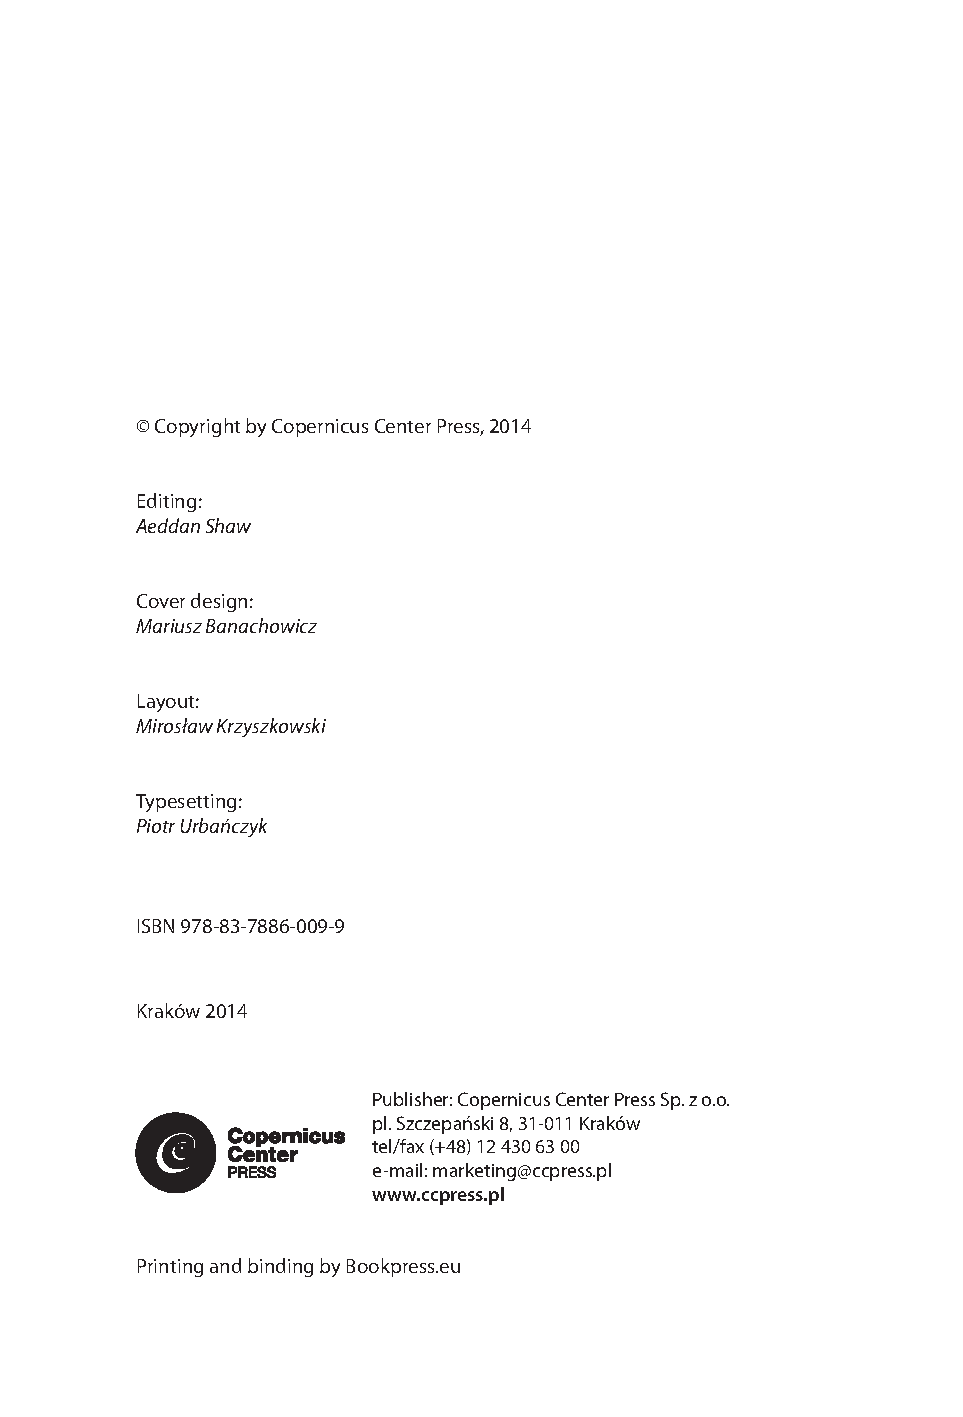
\includepdf[pages=1]{images/CT4.pdf}


\thispagestyle{empty}
\vspace*{1.2in}%
\begin{flushright}
\rectitle{Zagadnienia Filozoficzne\\w Nauce}\par
\vspace*{.5in}%
\chaptitleeng{Philosophical Problems\\in Science}\par
\end{flushright}
\vfill
\clearpage

\thispagestyle{empty}



\noindent\begin{czw}© Copernicus Center Press, \rok\end{czw}

\vfill

\urlstyle{sf}
\begin{adres}
	\begin{pagname}\noindent Except as otherwise noted, the material in this issue is licenced under the Creative Commons BY-NC-ND licence. To view a copy of this licence, visit \url{http://creativecommons.org/licenses/by-nc-nd/4.0}.
	
	\end{pagname}
\end{adres}
\urlstyle{rm}

%\urlstyle{sf}
%\begin{czwccp}
%\linespread{2.0}
%\noindent Except as otherwise noted, the material in this issue is licenced under the Creative Commons BY-NC-ND 4.0 licence. To view a copy of this licence, visit \url{http://creativecommons.org/licenses/by/4.0}.
%\end{czwccp}
%\urlstyle{rm}

\vskip1.5em

\vfill

\begin{adres}
	\begin{pagname}\noindent\begin{czwad}Editorial Board\end{czwad}\\
		Editor-in-Chief: dr hab. Paweł Jan Polak\\
		Deputy Editor-in-Chief: dr hab. Janusz Mączka\\
		Honorary Editor: prof. dr hab. Michał Heller\\
%		Guest Editors: dr Bartłomiej Skowron, dr Michał Eckstein\\
		Editorial Secretary: Piotr Urbańczyk
		
	\end{pagname}
\end{adres}


\vfill


\noindent\begin{czw}Proofreading: dr Roman Krzanowski\end{czw}

%\vskip.5em

\noindent\begin{czw}Adjustment and correction: Artur Figarski\end{czw}

%\vskip.5em

\noindent\begin{czw}Cover design: Mariusz Banachowicz\end{czw}

%\vskip.5em

\noindent\begin{czw}Technical editor: Artur Figarski\end{czw}

%\vskip.5em

\noindent\begin{czw}Typeset and typographic design: Piotr Urbańczyk\end{czw}

%\vskip.5em

%\noindent\begin{czw}Typeset in \end{czw}\LaTeX

%\noindent\begin{czw}Skład: Artur Figarski\end{czw}


\vskip1.5em

\vfill

\begin{adres}
	\begin{pagname}\noindent ISSN 0867-8286 (print format)\\
		e-ISSN 2451-0602 (electronic format)
	\end{pagname}
\end{adres}

\vskip1.5em

\vfill

\begin{adres}
		\noindent\begin{czwad}Editorial Office\end{czwad}
	
		\noindent\begin{pagname}Zagadnienia Filozoficzne w Nauce
		
		\noindent Wydział Filozoficzny UPJPII
		
		\noindent ul. Kanonicza 9, 31-002 Kraków
		
		\noindent POLAND
		
		\vskip.3em
		
		\noindent e-mail: zagadnienia@upjp2.edu.pl
		
		\noindent www.zfn.edu.pl\end{pagname}
\end{adres}

\vfill

\begin{wrapfigure}{L}{.3\textwidth}
	\noindent\includegraphics[width=.29\textwidth]{_images/ccp.pdf}
%\noindent\includegraphics[width=.27\textwidth]{images/ccp.pdf}
\end{wrapfigure}
\vskip.4em
%\noindent\parbox[t]{6cm}{
\begin{adres}
	\noindent\begin{pagname}Publisher: Copernicus Center Press Sp. z o.o.
		
		\noindent pl. Szczepański 8, 31-011 Kraków POLAND
		
		\noindent tel. (+48) 12 448 14 12
		
		\noindent e-mail: marketing@ccpress.pl
		
		\noindent www.ccpress.pl\\ \end{pagname}
	
	
\end{adres}
%}




\clearpage

%\input{toctest.tex}
%
%\clearpage

%Spis tresci -------------------------------------------------

{\thispagestyle{plain} \tableofcontents \clearpage}
%-------------------------------------------------------------
\newpage
\thispagestyle{plain}
\cleardoublepage
\thispagestyle{plain}

%-------------------------------------------------------------






%\input{default.tex}





%\sekcja{Od Redakcji}{Editorial}

%\input{EDI/editorial-PU.tex}



\sekcja{Artykuły}{Articles}

%\renewcommand{\theequation}{\arabic{section}.\arabic{equation}}
%\input{ART_Majid/Majid.tex} 
%\renewcommand{\theequation}{\arabic{equation}}


\begin{artengenv}{Igor Wysocki}
	{The problem of indifference and homogeneity in Austrian economics: Nozick's challenge revisited}
	{The problem of indifference and homogeneity in Austrian economics\ldots}
	{The problem of indifference and homogeneity in Austrian economics: Nozick's challenge revisited}
	{Nicolaus Copernicus University}
	{The pivotal point in the Austrian literature on homogeneity, choice and indifference was constituted by Nozick's \textit{On Austrian Methodology}. Nozick provoked a~long debate on the above notions within Austrianism. The aim of this paper is to elaborate such an account of \textit{homogeneity} that would take the sting out of Nozick's challenge and allow for non-trivial formulation of the law of diminishing marginal utility. Hence, we shall first take a~closer look at the debate on indifference within the Austrian camp, while defending and building upon the Hoppean account vis-à-vis Block's criticism. Our justification of the Hoppean position shall consist in showing that his account of the correct description of an action is not an \textit{ad hoc} move aimed at solving just one problem of indifference but is highly intuitive and widely applicable. We conclude by restating the above-mentioned law, thus demonstrating that the Nozickian objection can be successfully addressed.}
	{indifference, choice, homogeneity, Nozick's challenge.}



\section{Introduction }
\lettrine[loversize=0.13,lines=2,lraise=-0.01,nindent=0em,findent=0.2pt]%
{I}{}n 1977, Nozick wrote his seminal paper \textit{On Austrian Methodology}
%\label{ref:RNDps0Zfg5ToD}(Nozick, 1977)
\parencite[][]{nozick_austrian_1977} %
 thereby levelling a~challenge at the entire Austrian school of economics. Nozick's critique pertained to all sorts of claims Austrians made, ranging from acting on strict preference vs weak preference, through the doctrine of sunk cost and Austrian avowed apriorism, to their theory of time preference. However, it was Nozick's claim\footnote{This claim was even dubbed as Nozick's challenge by Hudik 
%\label{ref:RNDxYMAZoNHH3}(2011).
\parencite*[][]{hudik_note_2011}.%
} that, logically speaking, Austrian's formulation of the law of diminishing marginal utility must rely on the notion of indifference that stirred a~long-lasting and still inconclusive debate on the role of the said conception Austrian economics. This indictment by Nozick 
%\label{ref:RNDJay6TeejGy}(1977, pp.370–371)
\parencite*[][pp.370–371]{nozick_austrian_1977} %
 is so important for the entire Austrian edifice\footnote{As we are about to see, it is the very formulation of the law of diminishing marginal utility and the universal law of time preference that logically depends on the notion of indifference.} that it merits being quoted in full:

\myquote{
Indeed, the Austrian theorists need the notion of indifference to explain and mark off the notion of a~commodity, and of a~unit of a~commodity. If everyone or one person prefers one homogenous batch of stuff to another homogenous batch of the same shape of the same stuff (perhaps they like to choose the left-hand one, or the one mined first), these are not the same commodity. They will have different prices. Particular things $x$ and $y$ will be the same commodity (belong to the same commodity class) only if all persons are indifferent between $x$ and $y$. Without the notion of indifference, and, hence, of an equivalence class of things, we cannot have the notion of a~commodity, or of a~unit of a~commodity; without the notion of a~unit (‘an interchangeable unit') of a~commodity, we have no way to state the law of (diminishing) marginal utility.
}
Nozick's view is that the statement of the law of diminishing marginal utility presupposes the employment of the notion of indifference (or the one of the same commodity\footnote{The relation between the two is to be probed later. }). Therefore, it seems that homogeneity of economic goods is no mere epiphenomenon playing no role in praxeology as such. Quite the contrary, the notion of indifference is purportedly \textit{essential} for understanding the logic of human action. To appreciate the disagreement between Nozick and Austrians, it would suffice to realize that the Austrian dogma---adhered to by some of its most prominent figures, e.g. Rothbard and Block themselves---was that indifference is praxeologically irrelevant, and as such it cannot make any difference to human action. Or, in other words, man does not act on indifference. More specifically, Austrians of orthodox persuasion (Rothbard and Block\footnote{Block
%\label{ref:RNDaOh29qMnMU}(1980, pp.424–425, 1999, pp.22–24)
\parencite*[][pp.22–24]{block_austrian_1999} %
 conceives of indifference as ``vague, psychological category''.}) relegate indifference to the realm of mere psychology. Those insights were most tellingly captured by Rothbard 
%\label{ref:RNDkgop4g9o4w}(Rothbard, 2011, p.304)
\parencite*[][p.304]{rothbard_toward_2011} %
 in the following passage: ``Indifference can never be demonstrated by action. Quite the contrary. Every action necessarily signifies a~\textit{choice}, and every choice signifies a~definite preference. Action specifically implies the \textit{contrary} of indifference. The indifference concept is a~particularly unfortunate example of the psychologizing error.'' It is also Hoppe 
%\label{ref:RNDxufvb801ZV}(2005)
\parencite*[][]{hoppe_must_2005} %
 that wants to banish the concept of indifference out of the realm of human action. And it is precisely this relation of logical equivalence between indifference and no choice that constitutes the crux of the Hoppean 
%\label{ref:RNDou0qNn8Xuh}(2005)
\parencite*[][]{hoppe_must_2005} %
 solution. To put his point in still different terms, suppose we take a~set of various economic means and the equivalence relation (that of indifference) on this set. The relation of indifference would divide our original set into mutually disjunctive equivalence classes, which means that all the units in each class are the units between which the economic actor is indifferent. This in turn would mean that the actor cannot choose between the units within those equivalence classes. Conversely, if he can choose between any two units, these units must belong to distinct equivalence classes. Incidentally, we will revisit the original Hoppean solution when defending his account vis-à-vis Block's criticism in the forthcoming part of the present paper.

However, let us not precipitate things at that introductory stage. Instead, let us conclude the present section by setting the agenda for what is to follow. The present paper proceeds in this manner: section 2 takes the task of elucidating such critical concepts as \textit{indifference}, \textit{homogeneity} and \textit{same good}, with the relations between them being heeded too. Section 3 is dedicated to the detailed analysis of Nozick's challenge concerning the alleged necessity of the adoption of the concept of indifference within Austrianism. The burden of section 4 is to show the inadequacies of Block's attempt to deal with Nozick's problem. Section 5 tries to show the superiority of the Hoppean account of choice and indifference over Block's, while at the same time dispelling a~possible objection to the effect that the Hoppean solution is simply an ad hoc conceptual move designed to obviate one particular problem. Section 6 tries to extend Hoppe's conceptual framework in order to reformulate the law of diminishing marginal utility in a~way that apparently obviates Nozick's challenge. Section 7 concludes the paper.

\section{Mapping the conceptual terrain}
Before we move on to analyze the Nozick's challenge and to subsequently revisit the debate on indifference, as it unfolded within the Austrian camp, we need to clarify some critical concepts and straighten out possible misconceptions.

First and foremost, there is a~subtle terminological distinction that needs elucidating. So far, we have been using the words \textit{indifference}, \textit{homogeneity} or \textit{same commodity} (or \textit{same good} for that matter) in a~rather cavalier fashion and the inquisitive reader might wonder whether we treat them synonymously or there are possibly some more interesting relations between them. First, let us note that Austrians, as pretty much all economists, are concerned not with things (or physical objects) as such but with economic goods and the latter are only in the eye of a~beholder. The relation between things (the ones being able to satisfy potential human needs) and economic goods is that of inclusion. In other words, all economic goods are physical objects but not vice versa. What it takes then for a~physical object to count as an economic good is that it must be valued positively; or, it must be \textit{believed}\footnote{This very caveat related to the actor's \textit{beliefs} is of utmost importance here. It is because we maintain that Austrians, with their commitment to radical subjectivism, ought to reject the Mengerian
%\label{ref:RND2O00O2Xfht}(2007, p.52)
\parencite*[][p.52]{menger_principles_2007} %
 contention that a~thing can be ranked as a~good only when it has ``such properties as render the thing capable of being brought into a~causal connection with the satisfaction of this need.'' This is too strong a~requirement. If I~deal with some units that I~believe (even if falsely) satisfy the same list of ends, I~would be inclined to price them identically. Moreover, I~would believe that giving up one unit of this apparent supply would mean the resignation from the satisfaction of the least pressing need they are all believed to satisfy. Therefore, I~should not have any preference for giving up any particular (marginal) unit over any other. We contend that these implications are sufficient to find such units the ones of the same good. Incidentally, this radical subjectivism reflected in conceiving of things as means, that is in the contention that the sufficient condition for a~thing to become a~means is that the economic actor \textit{must merely believe} that it can serve his end, was aptly captured by Mises 
%\label{ref:RNDU4l21zwKmV}(1998, p.92):
\parencite*[][p.92]{mises_human_1998}: %
 ``Goods, commodities, and wealth and all the other notions of conduct are not elements of nature; they are elements of human meaning and conduct. He who wants to deal with them must not look at the external world; he must search for them in the meaning of acting men.''}
to be able to satisfy an \textit{actual human need} (or to use the parlance of neoclassicals: it must have positive utility). Therefore, economists are concerned with \textit{only this} subset of things which are economic goods. And for a~thing to constitute an economic good, what it takes is at least one economic actor that believes (falsely or not) that the physical object in question is able to satisfy at least one of his actual needs. Incidentally, note that given Austrian extreme subjectivism, no case can be made for any entailment between physical sameness and indifference (economic sameness). Machaj's
%\label{ref:RNDLusJVHw4CZ}(2007, p.232)
\parencite*[][p.232]{machaj_praxeological_2007} %
 celebrated example was that a~ring (of a~specific physical constitution) on one's fiancée's finger is not \textit{economically} identical with a~physically identical ring ``given to her by a~total stranger on the street.'' So, it looks as though physical sameness does not entail economic sameness. In other words, even if $x$~and $y$~are physically indistinguishable, $x$~and $y$~do not \textit{necessarily} constitute \textit{economically} homogeneous units. Or to use a~different jargon referring to \textit{the same fact}, even if $x$~and $y$~are physically identical (down to the level of particles), there may be some actor who may not be indifferent between the two. Instead, he may strictly prefer one over the other.\footnote{In other words, numerical identity might matter even in the absence of any qualitative differences between two objects.} Nor does indifference entail physical sameness. This statement is even more incontrovertible for it is readily imaginable that two units are \textit{slightly} physicallydifferent and yet, this difference cannot translate (by the lights of the economic actor) into an economic difference. In fact, we do not need to be so cautious with our examples here once we subscribe to the view that for units $x$~and $y$~to be subsumable under the rubric of the same economic good, it is enough that they are \textit{believed} to be equally serviceable in the eye of the economic actor doing the valuation. Suppose our actor believes (correctly or not) that---relative to his needs---an apple juice and mineral water are equally good; that is, he believes that there is no such end that an apple juice would satisfy but mineral water would not and vice versa. Granted, there are \textit{actually} many non-overlapping needs that apple juice and mineral water can satisfy but why should the economic actor care about it. These may not figure in his value scales either by virtue of the fact that the actor is unaware of these possible services the two goods might render or he might not value them at all. Such an actor would be prone to regarding apple juice and mineral water as \textit{economically} indistinguishable. If he were forced to give up a~unit of apple juice or the one of mineral water, he would be indifferent between the two. And crucially, given his beliefs, he would price them equally. Having established that physical sameness is logically independent of economic sameness, what is still left to explain is the relation between \textit{indifference} and \textit{homogeneity}. Here, following a~common parlance, we submit that one would be ill-advised to treat them synonymously. It appears to be intuitively clear that \textit{homogeneity} is a~relation between \textit{economic goods}, whereas \textit{indifference} is a~mental state (a belief) of an actor. Specifically, \textit{indifference} has such a~propositional content (believing \textit{that} $x$~and $y$ are economically identical) that it cannot motivate an actor to act on it. By contrast, \textit{homogeneity} is a~relation holding between \textit{economic goods}. However, remember that \textit{economic goods} are not mere physical goods. The former are in the eyes of an economic actor.\footnote{There are mind-boggling complications involved in counting the number of economic goods supervening on physical objects. Let us take the Rothbardian 
%\label{ref:RNDVGFaM8mwaJ}(2009, pp.73–74)
\parencite*[][pp.73–74]{rothbard_man_2009} %
 example with eggs and modify it slightly to illustrate our point. Suppose we have 3 eggs and let 1 egg serve the end of throwing it at our enemy's window (we have 3 of them, so we can throw one egg at one enemy's window). With 2 eggs we might already prepare scrambled eggs (which is our second most valued end) and with 3 eggs we might make an omelet. How many economic goods (given our value scale) do we have having 3 eggs? It looks as if we already have 3 of them since we can use all of them in order to annoy our enemies. Additionally, we have 3 distinct 2-egg combinations to make scrambled eggs (although there seems to be one \textit{type} of economic good here, with the marginal unit being \textit{a}~2-egg combination). So, do we already have 6 economic goods or four of them? The unit of 3 eggs put together constitutes a~separate economic good for it is only that large a~marginal unit that allows us to prepare an omelet. So in the end, how many economic goods do we have? Seven of them? The difficulty in counting seems to consist in two problems: a) do we count token economic goods or types of economic goods? and b) should we, when counting, add up \textit{all} marginal units (1 egg, 2 eggs and 3 eggs)? After all, all these units are not \textit{jointly} possible. In fact, if we decide to use all of our eggs to make an omelet, all other ends cannot be satisfied (no throwing eggs at windows, nor preparing scrambled eggs) as we would be left with no eggs. All in all, for the time being, we prefer to remain agnostic on these issues although they definitely merit a~separate paper.} So, the question arises: under what conditions would two physical units constitute the same economic goods? The answer seems all too obvious: only when an actor is indifferent between the two. So, the relation of equivalence appears to hold between an actor being indifferent between physical units $x$~and $y$~and these units being economically \textit{homogeneous}. In other words, when an actor is indifferent between physical units $x$~and $y$, this fact \textit{entails} that $x$~and $y$~are exemplary of \textit{the same commodity} (\textit{the same economic good} or \textit{economic homogeneity}). And vice versa, when physical units $x$~and $y$~are \textit{economically homogeneous}, this fact \textit{entails} that there is an economic actor who would be indifferent between these two. Note that Nozick's requirement for the same commodity is too strong. He demands that ``all persons are indifferent between $x$ and $y$.'' This however, given Austrian subjectivism, would be a~massive coincidence. To settle the issue that physical units $x$~and $y$ are a~part of the same supply, it would take establishing that literally all the persons are indifferent between the two---the sheer impossibility. Instead, Austrian economists must perceive the same supply as \textit{relative} to a~given economic actor. Physical objects $x$~and $y$~might be considered the same economic good by person A~but person B~might as well consider them economically distinct. What is more, person C~might find them both economic bads. Having said that, let us now proceed to interpret what putative formidability of Nozick's challenge consists in.

\section{The analysis of Nozick's challenge}
First and foremost, Nozick's challenge may be construed as a~\textit{purely logical} objection to Austrian repudiation of indifference. After all, remember, the gist of Nozick's objection was that without the concept of indifference, Austrians would be unable to formulate the law of diminishing marginal utility. Indubitably, in this respect Nozick is right. The law of diminishing marginal utility\footnote{Rothbard
%\label{ref:RNDKAEMqS2WIL}(2009, p.25)
\parencite*[][p.25]{rothbard_man_2009} %
 states the law of marginal utility very succinctly and very clearly indeed. His definition assumes the following form: ``Thus, for all human actions, as the quantity of the supply (stock) of a~good increases, the utility (value) of each additional unit decreases.''} has it that when we deal with a~supply of economically same units, each additional unit we value less; or, in other words, each additional unit is of lower utility. To put it formally, n+1\textsuperscript{th} unit of a~given supply is of lower utility than n\textsuperscript{th} unit. And conversely, n-1\textsuperscript{th} unit of a~given supply is of higher utility than n\textsuperscript{th} unit thereof. This in turn means that the utility of the marginal unit in a~smaller supply is higher than the utility of a~marginal unit in a~bigger supply of the same commodity.\footnote{In fact, this is the reason why Rothbard 
%\label{ref:RNDbP6IDCTIQ8}(2009, pp.21–23)
\parencite*[][pp.21–23]{rothbard_man_2009} %
 speaks of \textit{the law of marginal utility} instead of the law of \textit{diminishing} marginal utility. After all, as shown above, marginal utility may increase once the supply of a~good shrinks.} Hence, Nozick correctly notes that this law craves for an \textit{independent} understanding of the notion of homogeneity. For suppose, an Austrian proponent objects that there is no such logical requirement and that the notion in question may be defined \textit{within} the very law somehow along these lines: we can easily establish whether $x$, $y$ and $z$~are units of the same economic good and we would do so by checking whether these units obey the law of diminishing marginal utility. So, generally speaking, what an Austrian adherent would effectively say is that units of the same good are such units that obey the law of diminishing marginal utility. Incidentally, similar remarks would apply to Austrian formulation of the universal law of time preference.\footnote{Then again, we believe there is no clearer exposition of the said law than the following passage from Rothbard 
%\label{ref:RNDbHMVsaefRE}(2011, p.15):
\parencite*[][p.15]{rothbard_toward_2011}: %
 ``A fundamental and constant truth about human action is that \textit{man prefers his end to be achieved in the shortest possible time.} Given this specific satisfaction, the sooner it arrives, the better. This results from the fact that time is always scarce, and a~means to be economized. The sooner any end is attained, the better. Thus, with any \textit{given end} to be attained, the shorter the period of action, i.e., production, the more preferable for the actor. \textit{This is the universal fact of time preference}.''} Austrians hold that for one (and the same!) end,\footnote{Note that since we value means instrumentally (that is only as much as they contribute to the satisfaction of our ends), the universal law of time preference must \textit{derivatively} apply also to means. Since for any given end, we would rather achieve it sooner rather than later, we \textit{must} also prefer to employ (or come into possession of them) necessary means sooner rather than later.} each actor would prefer to achieve it sooner rather than later. Note, this law also presupposes the notion of the same good---but this time in a~sort of \textit{atemporal} way for it is the same economic good that is carried over time (we may obtain \textit{it} at t\textsubscript{1} or at t\textsubscript{2}). When asked how we should understand the concept of the same good presupposed by the universal law of time preference, an Austrian economist might reply\footnote{As brilliantly observed by an anonymous reviewer, the following analysis of the law of diminishing marginal utility does not imply that Austrians failed to formulate the law in non-trivial terms. This would indeed be uncharitable. Yet, our point is more modest. We claim that the law under consideration would be necessarily tautological unless we independently elaborate on the notion of homogeneity (same good), which is precisely what is going to be done in the forthcoming parts of the paper.} in a~similar fashion: we can easily learn whether $x_{1}$ (some economic good at t\textsubscript{1}) and $x_{2}$ (some economic good at t\textsubscript{2}) are the units of the same good. We would do so by checking whether an actor would \textit{now necessarily} prefer $x_{1}$ to $x_{2}$.\footnote{In fact, it was Rothbard 
%\label{ref:RNDGHTnn39SAL}(2011, pp.15–16)
\parencite*[][pp.15–16]{rothbard_toward_2011} %
 himself who resorted to this tautologous defense of the universal law of time preference, which is evidenced by the following passage: ``\textit{Time preference} may be called the preference for \textit{present satisfaction} over \textit{future satisfaction} or \textit{present good} over \textit{future good}, provided it is remembered that it is the \textit{same} satisfaction (or ``good'') that is being compared over the periods of time. Thus, a~common type of objection to the assertion of universal time preference is that, in the wintertime, a~man will prefer the delivery of ice the next summer (future) to delivery of ice in the present. This, however, confuses the concept ``good'' with the material properties of a~thing, whereas it actually refers to subjective satisfactions. Since ice-in-the-summer provides different (and greater) satisfaction than ice-in-the-winter, they are \textit{not} the same, but \textit{different} goods. In this case, it is different satisfactions that are being compared, despite the fact that \textit{physical} property of the thing may be the same.'' Whereas in the body of the text we considered the possible Austrian rejoinder in the form of saying that the same good can be conceptualized as the one that obeys the universal law of time preference, Rothbard merely contraposes by saying that if there is an apparent preference for a~future good (ice cream in summer) over a~present good (ice-cream in winter now), these two cannot constitute one and the same economic good. So, not only is the Rothbardian solution clearly circular, but also it gives the impression of fudging the notion of the same good. It may seem that whatever counterexamples to the law of time preference one may possibly come up with, Rothbard would rebut it by claiming that his critic invokes two distinct economic goods. This is yet another indication that an \textit{independent} concept of the same good is logically required.} But these two apodictically true statements come at a~price. For the consequence of the lack of the independent (of the laws in question) notion of the same good, would turn those laws into concealed tautologies. Consider yet again,

\begin{enumerate}[label=\arabic*), ref=\arabic*]
\item (\textit{the law of diminishing marginal utility}\footnote{We take the liberty of providing our own (and not Rothbardian) formulation of the law of diminishing marginal utility only because our version makes the ultimately tautologous character of the reasoning under consideration more conspicuous. Moreover, as conceded in footnote 12 above, the (explicitly) tautologous formulation of the law cannot be attributed to any particular Austrian.}): a~supply of economically same goods constitutes such a~collection of units that each additional unit therein is valued less than the previous unit, and
\item (\textit{the definition of a~supply of economically same goods}): what we here \textit{mean} by a~supply of economically same goods is such a~collection of units that each additional unit is valued less than the previous unit.
\end{enumerate}
Since any good definitions are equivalences and the \textit{definiens} may be substituted for \textit{definiendum} \textit{salva veritate}, let us substitute for ``a~supply of economically same goods'' in 1) our \textit{definiens} in 2). We would end up with

\begin{enumerate}[resume, label=\arabic*), ref=\arabic*]
\item A~collection of units that each successive unit is valued less than a~previous unit constitutes such a~collection of units that each successive unit therein is valued less than the previous unit.
\end{enumerate}
Now, it is clearly visible that 3) is a~tautology in its open form. Incidentally, if we were to understood the same good as the one that obeys the universal law of time preference, then this law in turn would be rendered equally uninformative. A~concealed tautology would turn into a~tautology in its open form via exactly the same reasoning (see: steps 1-3 above). So, the main thrust of Nozick's objection can be interpreted as saying that without an \textit{independent} notion of indifference, the law of diminishing marginal utility\footnote{As demonstrated in passing above, Nozick's objection would apply with the equal force to the universal fact of time preference too.} would be simply trivial. It would not state an interesting (and non-trivial) relation between \textit{two different properties} of units in question; 1) that of \textit{belonging to the class of economically same goods} and 2) that of \textit{being valued less and less on the margin} once the class in question has fewer and fewer members. By contrast, a~tautology would state a~trivial truth: a~property is identical with itself. In our case: the property of belonging to the class of economically same goods is the same as the property of belonging to the class of economically same goods. This, however, is a~far cry, to say the least, from stating a~meaningful economic law.

Second, we must also concede to Nozick that pricing of the commodity also seems to rest on the notion of indifference. Then, if Austrians fail to somehow accommodate indifference into their theory, this would have disastrous consequences for their entire conceptual edifice. After all, it must be borne in mind that the market (equilibrium) price of a~given product is a~function supply and demand. And the demand curve is but a~reflection of the diminishing marginal utility of a~given product. That is, the demand curve---rather unsurprisingly---slopes downwards because the more we have (of a~given product), the less we value marginal units. And it is precisely why we are ready to buy \textit{more} (of pretty much anything) \textit{only when} the successive units of the product in question cost less and less. Therefore, it is clear to see that the demand curve reflects the logic of diminishing marginal utility. Hence, Nozick is right. If we fail to reconcile the notion of indifference with the law of diminishing marginal utility, then, while having a~distorted notion of the law, our idea of the demand curve would be flawed too. And this in turn would adversely affect the concept of the market prince since the market price is a~function of the demand curve. Yet, we believe that all these problems can be overcome once we make the concept of indifference a~function of the correct description of an action,\footnote{As suggested to me by an insightful anonymous reviewer, the word ``correct'' in the Hoppean
%\label{ref:RNDvdXSfND9UE}(2005)
\parencite*[][]{hoppe_must_2005} %
 phrase ``correct description of an action'' does not refer to any normative standard. Rather, it is ultimately a~matter of fact. Indeed, ``correct'' description of an action captures the \textit{mentalist} (or \textit{internal}) aspect of action; that is, \textit{how} the actor herself conceives of what she is doing. Still in other words, the correct description of action picks up only those elements which were chosen and which were thus strictly preferred to perceived alternatives.} very much in the vein of Hoppe 
%\label{ref:RNDs0HkMV8FOe}(2005).
\parencite*[][]{hoppe_must_2005}. %
 And it is the building upon this author's account (simultaneously defending it against Block's objections) that we shall now turn to.

\section{Why Block's account of indifference is inadequate }
The first Austrian to recognize the force of Nozick's challenge was Walter Block. This is evidenced in the way Block
%\label{ref:RNDyO2aE2QNkN}(Block, 1980, p.423)
\parencite*[][p.423]{block_robert_1980} %
 acknowledges the gravity thereof before he even tackles indifference: ``I consider Nozick's next attempt to show the necessity of indifference as one of the most brilliant and creative criticisms that has ever been levelled against any aspect of Austrian theory.'' But how does Block try to take the sting out of Nozick's objection? Since we are going to suggest a~more satisfactory solution than the ones hitherto ventured within the debate on indifference,\footnote{There were many contributors to the debate on indifference within Austrianism, regardless of whether they \textit{directly} address the Nozick's challenge or not. These include---among others---Block 
%\label{ref:RND3n5dmV3XEv}(2009a; 2009b);
\parencites*[][]{block_rejoinder_2009}[][]{block_rejoinder_2009-1}; %
 Block with Barnett 
%\label{ref:RNDWddJwwPCCa}(2010);
\parencite*[][]{block_rejoinder_2010}; %
 Hudik 
%\label{ref:RNDtovz4gvpAQ}(2011);
\parencite*[][]{hudik_note_2011}; %
 Rothbard 
%\label{ref:RNDOLaOHxWcv2}(Rothbard, 2011).
\parencite[][]{rothbard_toward_2011}. %
 Moreover, less characteristically within Austrianism, there is a~dissenting view to the effect that praxeology should embrace acting on \textit{weak preference} (rather than strict one), and thus possibly also on \textit{indifference}. This view is represented by, e.g., Machaj 
%\label{ref:RNDcRCVqlEmB4}(2007);
\parencite*[][]{machaj_praxeological_2007}; %
 O'Neill 
%\label{ref:RNDS9hQVdLlfc}(2010).
\parencite*[][]{oneill_choice_2010}. %
 The reason the present paper focuses on the discussion between Block and Hoppe is that, first, these two authors are particularly eloquent in presenting their respective (and contrasting) views; and second, they by far contributed most to the entire debate in question.} Block's 
%\label{ref:RNDhxhI3qux8E}(Block, 1980, pp.423–424)
\parencite*[][pp.423–424]{block_robert_1980} %
 wrestling with the challenge merits being quoted in full

\myquote{
Suppose that, for example, a~person has a~stock of some commodity. This means, of course, that he considers each unit equally useful, desirable, serviceable\ldots Let us presume that he has 100 lbs. of butter and now for some reason desires to give up one of these units of butter. And let us say, further, that he arbitrarily picks one such unit, say, the 72\textsuperscript{nd} one. Nozick would say that ‘the person does not prefer giving up this one to giving up another one' [\ldots]. But this interpretation is clearly unsatisfactory. For if the person didn't really prefer to give up this (72\textsuperscript{nd}) one, why did he pick it to be given. So. we are forced to conclude that the butter units were not really interchangeable from the point of view of an actor involved in the selection process. Thus, we seem to be forced to deny that there is ever any such thing as a~commodity, surely a~ludicrous position.
}
And we concur. Surely, it is a~ludicrous position; yet, it is precisely what Block's account is doomed to conclude for it is inherently unable to square the two apparent facts: 1) that those units of butter are \textit{really} (\textit{ex hypothesi}) ``equally useful, desirable, serviceable'' and 2) that 72\textsuperscript{nd} one was ‘picked up'.\footnote{Now, we must make a~slight concession in order to avoid begging any questions at this point. The concept of ‘picking up' does not conveniently play on the equivocation between preference and indifference since it unambiguously suggests the former. Our point, by contrast, is to say that somehow (in a~sense) 72\textsuperscript{nd} unit of butter was ‘picked up' but this notion of picking up is sort of \textit{non-preference implying} (or, positively speaking, indifference-implying). As noted, however, the notion of ‘picking up' (as commonly used) A~over B~implies that we prefer A~to B; after all, we want preferences to guide actual choices. As it will transpire, what captures the above scenario (with pounds of butter) much better is the description that 72\textsuperscript{nd} unit was not chosen (or picked up for that matter) at all. Yet, let us not precipitate things. We will come to this issue once we tackle Hoppe's account.} As we are about to see, the whole problem trades on the concept of ‘picking up'. Block seems to be lured into thinking that the imagined actor \textit{does} pick up the 72\textsuperscript{nd} unit where he says: ``For if the person didn't really prefer to give up this (72\textsuperscript{nd}) one, why did he pick it to be given''. Fair enough, if we \textit{assume} that he did pick up\footnote{Then again, the notion of ‘picking up' invoked here is the normal \textit{preference-implying} one.} this very unit, he must have preferred giving up this one to giving up any other, which simply logically follows from the concept of ‘picking up' employed herein. And yet, why should we beg any questions? It is to be established first that the actor \textit{does indeed} pick up the 72\textsuperscript{nd} unit. For settling this issue has a~bearing on whether he prefers giving this unit to any other or he does not. And this in turn determines whether the actor conceives of the 72\textsuperscript{nd} unit as the unit of the same supply (with all the other units of butter) or he conceives of the stock before him as consisting of two distinct classes: a) a~homogeneous class of 99 units (still intact) and b) a~singleton containing the very pound of butter given up.\footnote{We still hasten to add that ‘given up' here should not imply that the very item was dispreferred. The correct description of the action in case (and that is the point we shall press in the forthcoming part of the paper) all 100 units were perceived as equally serviceable is that the actor could not---logically speaking---choose between them.} Therefore, it seems that something has to give here: either 100 units were not in fact perceived as equally useful or they indeed were but the actor did not (in a~relevant sense) choose to give up the 72\textsuperscript{nd} unit. So, Block cannot have it both ways. But before we embark on further considerations, let us cite the apparent solution Block
%\label{ref:RNDMIRKfOUG10}(1980, p.424)
\parencite*[][p.424]{block_robert_1980} %
 offers:

\myquote{
I~think that this problem can be reconciled as follows. \textit{Before} the question of giving up one of the pounds of butter arose, they were all interchangeable units of the commodity, butter. They were all equally useful and valuable to the actor.

But then he decided to give up one pound. No longer did he hold, or can he be considered to have held, a~homogeneous commodity, consisting of butter pound units. Now there are really two commodities. Butter\textit{\textsubscript{a}}, on the one hand, consisting of 99 one-pound units, each (of the 99) equally valued, each interchangeable from the point of view of the actor with any of the other in the 99-pound set: on the other hand, butter\textit{\textsubscript{b}}, consisting of one pound of butler (the 72\textsuperscript{nd} unit out of the original 100 butter units, the one, as it happens, that he chose to give up when he desired to sell off one of his pounds of butter). In this case butter\textit{\textsubscript{a}} would be preferable to butter\textit{\textsubscript{b}}, as shown by the fact that when push came to shove butter\textit{\textsubscript{b}} was jettisoned and butter\textit{\textsubscript{a}} retained.
}
We will offer two interpretations of the above passage. One perusal will construe of what Block seems to mean literally, whereas the other will attempt to interpret him charitably, thus rendering Block's statement true but irrelevant. So, as hinted at above, Block seems to imply that \textit{the choice} constitutes a~sort of breaking point, after which there are no longer homogenous units but the formerly homogenous collection is now divided into two sets: in one of them we still have homogenous units and the other set is a~singleton, with the element not being homogenous with the remaining elements in the previous set. The problem with this contention is that Block must either invalidate his assumption that they were homogeneous before the choice in order to explain why the choice (i.e. picking up the least preferred unit of butter, as opposed to the remaining ones) took place. Alternatively, if he maintains that the units in question are indeed equally useful, then he cannot explain why this particular unit of butter was picked up because they were assumed to be equally valuable in the first place. Nozick's challenge comes with vengeance to Block and the reason is precisely that the latter author has a~distorted idea of choice.\footnote{This idea of choice is going to be remedied by Hoppe
%\label{ref:RNDysvIpjR6ZD}(2005),
\parencite*[][]{hoppe_must_2005}, %
 as we are about to see.} To appreciate this indictment of ours more clearly, let us press the problem of choice (and \textit{what exactly} is chosen) a~bit harder. What prompts Block to believe that it was the 72\textsuperscript{nd} unit---as opposed to just \textit{a}~unit---that was given up in the above-considered scenario? We would like to venture a~hypothesis that Block (however implicitly) could have believed that whatever made the sentence ``72\textsuperscript{nd} unit was exchanged for money'' true (with the truth-maker in question being the entire action-token in which all the details are provided: there was a~particular unit exchanged for a~particular banknote at a~particular time and space via particular bodily movements etc.) \textit{is the same} as the propositional content of the actor's intention. But this is highly improbable. This would predict that---at least in this case---there was only \textit{one possible} (and extensionally defined) \textit{state of affairs} which would satisfy the actor's intention. If Block were to think so, he would wind up advocating perfect heterogeneity of means, being left with no hope of intelligibly conceiving of \textit{the same commodity}. After all, choices reflect strict preferences and if everything (down to the level of the most minute details) is chosen, then at least for this actor, the supply of the same commodity is an empty category.\footnote{Strictly speaking, the equivalence classes of the same commodity would be always singletons.} However, it seems quite obvious that the actor's desire can be satisfied in an almost infinite number of ways. If we want to buy bread in a~local supermarket, it might be the case that we are indifferent even between supermarkets (because, say, they are equidistant and almost qualitatively identical) or between types of bread etc.---not to mention that it would be absurd to claim that we choose every single detail of our route to a~supermarket.\footnote{The same---rather commonsensical---point was pressed by Davidson 
%\label{ref:RNDGqeTcajk0A}(1963, p.688):
\parencite*[][p.688]{davidson_actions_1963}: %
 ``If I~turned on the light, then I~must have done it at a~precise moment, in a~particular way---every detail is fixed. But it makes no sense to demand that my want be directed at an action performed at any one moment or done in some unique manner. Any one of an indefinitely large number of actions would satisfy the want, and can be considered equally eligible as its object.''} So, there are infinitely many bodily behaviors and infinitely many routes that would do equally well from the actor's perspective. Now, combing these two infinities would yield a~Cartesian product, with every member thereof being equally good for that actor. In other words, any combination of a~particular route and a~particular bodily behavior under consideration would do as well as any other \textit{relative to the satisfaction of his particular intention}. Concluding, it would be a~fatal mistake to confuse \textit{a~particular state of affairs} (as specified in extensional terms)which actually occurred with \textit{a~content of the actor's intention}, with the latter being almost always intensionally specified. Granted, the content of the latter is propositional but the proposition (\textit{that} this or that happens) is normally satisfied by infinitely many particular states of affairs---but not by only one. And because the actor's intention can be satisfied in so many various ways, he \textit{must} be indifferent between some aspects of this multitude of states of affairs. And because he is indifferent between them, he does not choose between them. Having established that this possible retort Block might have availed himself of would not succeed either, let us move to the second perusal of the above-cited fragment from Block.

On the second reading, Block's position may be rendered true but then it would amount to the mere restatement of the law of marginal utility. In other words, what Block might mean is that \textit{after the choice}\footnote{But now, it is rather a~choice between having an exchange (of a~unit of butter for money) or refraining from it.} of a~particular unit of butter out of 100 of them we deal with a~new supply of 99 units thereof. Before any action was taken, the marginal value of each of those units was the least important goal each of them could satisfy. Now, whichever unit was gotten rid of, the marginal value of the remaining units must have increased. Hence, if Block ends up with 99 units of butter, it is a~matter of course that now the value of each of them (that is of a~marginal unit) is higher than what it was when he had 100 of them at his disposal. Yet, as indicated above, this is tantamount to the mere restatement of the law of marginal utility and therefore irrelevant.\footnote{Note that if Block's response is read as the mere restatement of the law of marginal utility, then it might be argued that it is not only irrelevant to the problem at stake but also question-begging: the response is called upon to vindicate the law of diminishing marginal utility against Nozick's challenge, yet it depends for its success on the restatement of the law as a~valid one. Furthermore, as we shall argue towards the end of the paper, the law in question is best understood, when grounded in the Hoppean correct description of an action and supplemented by sound counterfactual reasoning.} Specifically, it yet again fails to explain why the choice---as Block claims---of this particular unit took place. Having said that, it is about time to go on to consider the Hoppean account of choice and indifference.

\section{Hoppe's account as a~remedy for Block's shortcomings }
In this section, we are going to argue for two points: a) not only can a~choice be modelled in such a~way as to logically exclude the possibility of choice under indifference and b) there are additional reasons why we should endorse the Hoppean correct description of an action. We are going to stress on multiple occasions that it is not the case that the Hoppean account is just an \textit{ad hoc} proposal aimed at solving the problem of indifference, for if it were so, it might be claimed that Hoppe does not solve the problem of indifference and apparent choice among the units of the same supply but simply assumes it away: after all, Hoppe suggests understanding choice as such that it necessarily excludes indifference.

Let us now try to determine whether the Hoppean
%\label{ref:RNDtGo60RAdi2}(2005)
\parencite*[][]{hoppe_must_2005} %
 account fares any better when confronted with Nozick's challenge. First and foremost, it must be noted that---unlike Block's solution---it involves both doing justice to indifference\footnote{It should be constantly borne in mind that, after all, according to the majority of Austrians, indifference is not a~praxeological concept (see: footnote 17). This is due to the fact that indifference cannot be demonstrated in action, as is usually reiterated by Austrians 
%\label{ref:RND2SChO9KDOw}(see Block, 2009a; Block and Barnett, 2010; Rothbard, 2011).
\parencites[see][]{block_rejoinder_2009}[][]{block_rejoinder_2010}[][]{rothbard_toward_2011}. %
 By no means can we deduce from any actual choice whether we were confronted with the units of the same good or with the ones of distinct goods. } (at least admitting that a~man can be genuinely indifferent between some options) and barring it steadfastly from the realm of choice. Briefly speaking, Hoppe 
%\label{ref:RNDqcsL91XFnk}(2005)
\parencite*[][]{hoppe_must_2005} %
 maintains that one \textit{cannot} make a~choice under indifference. This ``cannot'' is definitely of logical nature and so, the truth of the proposition that a~man cannot choose when indifferent derives its truth solely from its constituent concepts. Specifically, Hoppe \textit{defines} choice in such a~way that it entails the lack of indifference. That is, if man chooses $x$ over $y$, he is not (and, logically speaking, \textit{cannot}) indifferent between the two. And conversely, he defines indifference in such a~way that the very fact that the actor is indifferent between $x$ and $y$ implies that he does not (and \textit{cannot}) choose between the two.\footnote{Then again, if this were all there is to the Hoppean account, it would hardly count as a~solution to Nozick's challenge. By contrast, Hoppe does indeed appeal to Searle's 
%\label{ref:RNDlGOI33r05g}(1984)
\parencite*[][]{searle_minds_1984} %
 distinction between internal-mentalist and external-behaviourist aspect of one's action, which definitely provides an independent reason counting in favour of the former's solution to the problem of indifference (vis-à-vis choice) in Austrian economics. In the forthcoming part of this section, we are going to build upon and thus sharpen Hoppe's (Searle's) insight by demonstrating that the there is a~deep distinction between \textit{a~description of one's action under such an aspect that makes it intentional} and \textit{the description of what one did} (whether intentionally or not). As we shall argue, the former captures not only the idea of what is chosen but also accounts for which maxim one acts on, thereby making it very useful in the assessment of the moral worth of one's actions. Briefly speaking, our agenda henceforth is to show that the Hoppean solution involving the correct description of an action is a~powerful explanatory device shedding light on many aspects of human life, while not being a~mere stipulative \textit{ad hoc} move (the definitional exclusion of indifference from the realm of choice) aimed at saving Austrian economics from Nozick's challenge.}

Based on the original Hoppean account just adduced, the following two relations must hold:

\begin{enumerate}
\item an actual choice between units $\rightarrow$ strict preference for one of the units;
\item indifference between units $\leftrightarrow$ no possible choice between the units.
\end{enumerate}
At this point, we would do best to obviate one possible objection that might be raised against Hoppe. Note that it might be claimed that it can surely be the case that one cannot choose $A$ over $B$ \textit{even if} one is not indifferent between the two and the reason might be that $A$ is unavailable. Then it would look as though it is only indifference that entails the impossibility of choice, whereas the impossibility of choice would fail to entail indifference. However, this merely psychological (in the absence of action) fact that an actor prefers $A$ over $B$ would be of no interest to Austrian economics with its commitment to the doctrine of demonstrated preference
%\label{ref:RNDZeuhzEUrWg}(see \textit{inter alia} Rothbard, 2011).
\parencite[see \textit{inter alia}][]{rothbard_toward_2011}. %
 Simply stated, the actor's preferences that cannot be demonstrated in action are not part and parcel of this school of thought. Therefore, whenever we speak of the possibility of choosing $A$ over $B$, this presupposes that both $A$ and $B$ are available. And that is why the only reason why an actor cannot choose (given our presupposition) between $A$ and $B$ is that he is indifferent between them. And this why it is the relation of equivalence that holds between indifference between some units and an inability to choose between them. Having preempted this possible rejoinder, let us cite some textual support confirming that Hoppe 
%\label{ref:RNDXeoNeneUn0}(2005, p.91)
\parencite*[][p.91]{hoppe_must_2005} %
 indeed perceived the relation between choice and difference in the way reconstructed above:

\myquote{
Likewise, a~mother who sees her equally loved sons Peter and Paul drown and who can only rescue one does not demonstrate that she loves Peter more than Paul if she rescues the former. Instead, she demonstrates that she prefers~\textit{a}~(one) rescued child to none. On the other hand, if the correct (preferred) description is that she rescued Peter, then she was not indifferent as regards her sons.
}
Clearly then, if the mother chose (the preferred description) to save Peter, she thus demonstrated the strict preference for him over Paul, which exemplifies relation 1) cited above; whereas the relation 2) is most tellingly (however indirectly) elucidated with the proverbial Buridan's ass wavering over two identical bales of hay
%\label{ref:RND3KkT0Yhgia}(Hoppe, 2005, p.91):
\parencite[][p.91]{hoppe_must_2005}:%


\myquote{
Lastly, consider Buridan's ass standing between two identical and equidistant bales of hay. The ass is not indifferent and yet chooses one over the other, as Nozick would have it. Rather, it prefers~\textit{a}~bale of hay (whether it is the left or the right one is simply not part of the preferred choice description), and thus demonstrates its general preference of hay to death.
}
The relation 2) can easily be inferred therefrom: the ass being indifferent between these two bales of hay, did not \textit{choose} between them; rather, he chose \textit{a} hay over death, which, eventually, implies its preference for the former over the latter. Having said that, it is high time to ask what are the merits (or demerits?) of the Hoppean account? And in particular: why is the Hoppean account superior to Block's and how does former address Nozick's challenge? To test Hoppe's position, let us apply it to the scenario of giving up a~pound of butter cited above.

There are two logical possibilities here. If the actor views all 100 units of butter as genuinely equally serviceable, then all of them fall into the rubric of the same economic good. Then \textit{any} correct description of his action would not involve any choice \textit{between these units}. It is certainly the case that it is strict preference that guides the actor's choice; yet, this choice is not between the units assumed to be equally serviceable.\footnote{Remember, all these units would then fall into the same equivalence class (with indifference between the equivalence relation dividing all economic means into mutually disjoint classes) \textit{within which} an actor does not (and cannot) choose.} It is this very point that Block does not concede, thereby running into all the above-mentioned conceptual problems. So, positively speaking, how to account for the transaction that occurred? The solution seems fairly straightforward: since the actor \textit{did} indeed give up the 72\textsuperscript{nd} pound of butter (while holding all of them equally serviceable), he must have preferred giving up \textit{a}~unit of butter for some pecuniary equivalent. In other words, the actor preferred one unit of butter less, but some increment of money to retaining his entire stock of butter but depriving himself of an opportunity to earn this money. The second possibility is that the correct description of an action is that the actor really dispreferred that 72\textsuperscript{nd} unit that he actually gave up. If so, that unit was not the same economic good as all the other units in the first place and therefore, trivially, the original supply of 100 units was heterogeneous. At the very least, there were at least two classes of economic goods involved as the unit actually given up was \textit{ex hypothesi} (due to the correct description of the action) valued less than any other.

For the time being, let us return to the celebrated Hoppean thought experiment with mother saving either Peter and Paul from drowning and let us suppose that Block could still argue that the mother could not be indifferent between Peter and Paul under any circumstances once she saved Peter. The bone of contention then would be \textit{the act of saving Peter} and whether the fact that the mother (at least according to one description of her action) did save Peter in turn implies that the mother did indeed choose to save Peter. Let us analyze more closely this tack that Block might try. Block's point against Hoppe would be decisive if the act of \textit{saving a~particular child} (under this description) instead of another were inherently \textit{preference-implying}. That is, Block would succeed if we can infer from \textit{the fact} of saving a~particular child (or from bringing about the event of a~particular child being saved) that this particular child was preferred to the other. Yet, there is a~deep distinction favored by Davidson
%\label{ref:RNDQz9TpqEE9X}(Davidson, 2001)
\parencite*[][]{davidson_agency_2001} %
 between \textit{what an actor does} (including his primitive action consisting in his bodily movements up to everything they cause) and what he does \textit{intentionally}. As Davidson 
%\label{ref:RNDBeItpdWezQ}(2001, p.45)
\parencite*[][p.45]{davidson_agency_2001} %
 put it: ``[…] although intentionality implies agency, the converse does not hold.'' Therefore, it would simply beg the question to say that by the act of saving Peter the mother demonstrated her preference for Peter over Paul. As established above by alluding to the Davidsonian insight, from the event that the mother authored, we cannot infer \textit{which aspects thereof were informed by her preference}. Therefore, not to beg any questions, we should treat the act of saving Peter in \textit{the non-choice}---(and hence also non-preference)---\textit{implying} sense. Alternatively, just to remain neutral on whether the mother did actually choose to save Peter or chose to save \textit{a} child, we could say that what the mother \textit{in fact did} was to save Peter. After all, to say that the mother saved Pater is only \textit{to attribute her agency} to this event (in other words, it is to say that she \textit{authored} the event of Peter having been saved), which does not imply that she saved Peter \textit{intentionally.} Andthis is the key insight which, in our view, counts in favor of the Hoppean account. Just to reiterate, there is a~distinction to be drawn between the authored event (Peter being saved) and this description of the mother's action that makes it intentional (e.g. saving \textit{a}~child). It is only the latter description that accounts for what the mother intended to do, and hence chose. Therefore, we can easily conclude that it is only \textit{some aspects} of the authored event that an actor intentionally brings about or chooses to bring about. For example, assuming that the latter description is a~correct one, the mother was not choosing between her children, although it is true what she \textit{in fact did} was to save Peter. Finally, authored events are defined in extensional terms (with all minute details being fixed), whereas the actor's intentions (strictly speaking, their propositional content) is envisaged in intensional terms. And it is what Hoppe 
%\label{ref:RND2rGixACIkS}(2005)
\parencite*[][]{hoppe_must_2005} %
 hints at throughout his paper: it is the idea that what the actor genuinely \textit{chooses} is reflected in his (from his privileged first-person point of view) preferred description of the action.

To further reinforce the Hoppean point of the correct description of an action, we can also resort to Parfit's
%\label{ref:RNDnoqSHnRa1e}(2011, p.289)
\parencite*[][p.289]{parfit_what_2011} %
 incisive remarks (though literally located within the context of Kant's philosophy) related to the issues of adequately describing on what maxims people actually act:

\myquote{
Whether some act is wrong, Kant's formulas assume, depends on the agent's maxim. Of the maxims that Kant discusses, most involve some policy, which could be acted on in several cases. Two maxims may be different, though they involve the same policy, because they involve different underlying motives or aims. Two merchants, for example, may both act on the policy ‘Never cheat my customers'. But these merchants act on different maxims if one of them never cheats his customers because he believes this to be his duty, while the other's motive is to preserve his reputation and his profits.
}
This quote could aptly illustrate our (and Hoppean) intuition that two identical behaviors could then translate into two distinct actions, depending on the way we frame our goals. Or to use Parfit's language, the actor's observed particular behavior cannot unambiguously point to a~maxim he is acting upon for the former may be compatible with practically infinitely many varieties of the latter. After all, the relation between a~maxim and behavior is many-to-many. A~given maxim an actor is acting upon may be instantiated in infinitely many behaviors and vice versa: as we say, a~given behavior may translate into many maxims. And now, the way of getting to a~correct description of an action was brilliantly illuminated by Parfit
%\label{ref:RNDA4keeRzY8A}(2011, pp.289–290).
\parencite*[][pp.289–290]{parfit_what_2011}. %
 The author considered acting on the following highly specific maxim: stealing some wallet from some woman dressed in white who is eating strawberries while reading the last page of Spinoza's \textit{Ethics}. Ethical objections connected to acting on such rare maxims aside, the author suggested the following to determine which maxim is actually guiding our actor:

\myquote{
This objection can be partly answered. Just as it is a~factual question what someone believes, or wants, or intends, it is a~factual question on which maxim someone is acting. And real people seldom act on such highly specific maxims. When we describe someone's maxim, as O'Neill and others claim, we should not include any details whose absence would have made no difference to this person's decision to do whatever he is doing. In a~realistic version of my example, I~would have stolen from my victim even if she had been dressed in red, or had been eating blueberries, or had been reading the first page of \textit{Right Ho Jeeves}! My real maxim would be something like ‘Steal when that would benefit me.'
}
So now, do not the above considerations perfectly correspond with the Hoppean distinctions between choice, indifference and the correct description of an action? To put it more specifically, it should by now seem obvious that physical objects $A$ and $B$ cannot constitute two distinct economic goods when they do not figure in the correct description of an action. In other words, whether $A$ or $B$ is employed \textit{cannot make a~difference} to the actual maxim we are acting on. If our maxim (preferred description of an action) is to save \textit{a}~child, it simply follows that any child would do equally well. The mother cannot be rendered worse off when Peter (or Paul for that matter) is saved simply because both of these scenarios count as the satisfaction of the very same policy of ours. And that is the reason these two (only seemingly distinct) goods are actually the same economic good and it is precisely for the very same reason that we do not choose between them.\footnote{First, it appeared as if indifference between $A$ and $B$ analytically entailed the impossibility of choosing between $A$ and $B$ (what we christened Hoppe's stipulative move). Now it seems we found another reason why indifference between two units and the impossibility of choosing between them must go hand in hand.}

Finally, let us note that Nozick's challenge leaves the Hoppean position unscathed. Nozick's point is simply irrelevant once we subscribe to the Hoppean account of choice. To conceptualize a~supply, Austrians have to employ the notion of indifference---fair enough. Yet, whenever any two units are the units of the same commodity, they shall never figure in a~description of one and the same action. In other words, once any two items represent the same economic good, there is no choice between them. Therefore, a~choice under indifference---an anathema to Austrians---is rendered impossible now. We might also put the above point in the jargon of philosophers of actions, when two---economically identical---goods are at stake, our goal (maxim) is satisfied to the same degree regardless of whether one good or the other is employed. Since the correct description of an action might be mute on the employment of a~\textit{particular} good (as opposed to the use of a~\textit{type} of good), it follows that two \textit{numerically} distinct physical items being equally serviceable in the performance of an action in question must count as the same economic good simply because \textit{the satisfaction conditions} of our actions\footnote{These, of course, follow from the correct description of an action.} do not discriminate between these two units.

\section{Extending the Hoppean framework: stating the law of diminishing marginal utility }
Before we sharpen the formulation of the law of diminishing marginal utility, we need to take heed of one conceptual trap we might fall into. As we were pointing out throughout the paper, the meaningful (non-trivial) formulation of this law depends on the independent notion of the same economic good. Additionally, we posit that a~given stock of units may be considered by an economic actor as a~supply of \textit{the same commodity} only relative to a~given moment. Strictly speaking, it is a~matter of course that human action is sequential (in a~temporal sense) by nature; yet, an actor at t\textsubscript{1} may envisage the way he is going to employ consecutive units at later times. This \textit{double time indexation}---one standing for a~given moment in which an actor envisages the employment of his successive means and the other standing for the \textit{actual} time at which they are employed---is necessary. For suppose \textit{arguendo} that our only time indexation is the time of the \textit{actual} employment of the means for the satisfaction of our goals.Then, we submit, the hope of formulating the desired law would be forlorn. In fact, if we apply the said single index, we would observe that the marginal utility increases once we deal with fewer and fewer units. Certainly, it is impossible to still speak of the same commodity when the marginal utility varies. So, generally speaking, if we have nunits of apparently the same commodity, and once we employ the n\textsuperscript{th} one, we end up with the supply of n-1 units. The marginal utility of the latter supply is higher than in the original one. However, even the above statement is one not entirely correct. For, remember, to state that the marginal utility diminishes once the supply gets smaller and smaller, it must be \textit{the supply of the same economic good}. As we can see, \textit{the single indexation} would not enable us to formulate the law of diminishing marginal utility. Rather, it would depend on the very law we are trying to formulate. Note, our aim still is to develop a~robust notion of a~supply of the same commodity. Only then can we show that marginal utility would indeed increase once the said supply shrinks.

So, just to introduce our allegedly necessary double indexation, let us put forward the following notation. As promised, each unit is to be indexed for time twice in the following manner:

\begin{enumerate}
\item It is going to be indexed \textit{for the time of its actual employment}, with the time being indicated in the subscript. So, u2\textsubscript{3} is to be read as \textit{the second unit} employed at t\textsubscript{3} (time 3).
\item Additionally, it is going to be indexed \textit{for the moment in which an actor imagines its future employment}, with this moment being indicated in the superscript. So, adding to our previous example,
%u2\textsubscript{3}\textsuperscript{1}
u2$_{3}^{1}$ is to be read as how an actor imagines at t\textsubscript{1} how the second unit is to be employed at t\textsubscript{3}. Note, we allow the time variables in both indices to range from the present (t\textsubscript{1}) onwards up to the conceivable future. Yet, the time of envisaging the employment of the units must be earlier than the actual employment of the units. In other words, the natural number in the superscript must be lesser than the number in the subscript. After all, intuitively speaking, once a~means was utilized, there is nothing to economize any longer.
\end{enumerate}
So, armed with the above formal notation and having in mind the condition that given units can be viewed as constitutive of a~supply of the same commodity only \textit{relative to a~given moment}, we can now state what it is for a~given set of units to be perceived as economically identical. What would, for example, make u1 and u2 units of the same commodity, as viewed now (at t\textsubscript{1}) by an economic actor? Formally speaking, it would mean that for any t~(in the subscript, which is the time of the actual employments of these units), the actor is indifferent (\textit{now}) between 
%u1\textsubscript{t}\textsuperscript{1}
u1$_{\text{\,t}}^{1}$
and
%u2\textsubscript{t}\textsuperscript{1}
u2$_{\text{\,t}}^{1}$.
To put it verbally, at least as of now, the actor believes that he can swap these units in any time in the future without any loss of utility (or satisfaction for that matter). Still in other words, he \textit{now} believes that it is a~question of indifference whether he employs u1 at any time instead of u2 at that time. Note that we can easily understand that a~unit can preserve its \textit{economic} identity over time, which, incidentally, does not run counter to the universal fact of time preference. After all, we assume as a~correct description of our consecutive actions that a~given unit (say, u1) over certain time is equally serviceable as any other unit in our set. If an actor believes that u1 can be put to use at t\textsubscript{1} as well as at, say, t\textsubscript{8}, then there is no preference for the employment of this unit now to its employment later. By no means does that threaten the universal law of time preference. Quite the contrary, when we genuinely find (now) some set of units equally serviceable across a~given range of time, then, logically speaking, these units are viewed as economically identical \textit{across that time.} In other words, for any unit in that set, there is no preference for its use at any particular time over any other. When it comes to the satisfaction of ends, the situation is diametrically different. We do satisfy our ends in a~descending order of their importance over time. Yet, our means are \textit{believed} (correct description of an action) to be equally serviceable over that very time. By assumption then, any of the said units can be equally well employed at any time.

Let us represent our rather intuitive findings more rigorously and generally. Let S~be a~set of n~number of units, which are believed to be equally serviceable. Let e~be a~number of ends each of the units is \textit{believed} to be able to satisfy equally well. Let also n~${\leq}$ e. The last requirement is important for if n~were greater than e, then some of the units in S~would not count as economic goods (for a~proper subset of S~would already satisfy all the ends the means are supposed to be able to satisfy). Now as long as we consecutively allocate any of these units to less and less important ends (starting from the most important one), then there are e! number of scenarios an actor would be indifferent to.\footnote{The number of ends unsatisfied will be e-n. These will be the ends figuring at the bottom of the actor's value scale. Furthermore, as we can see, the Hoppean account can be given a~temporal dimension. Now we can say not only that saving Peter is as good as saving Paul \textit{now} but also that some (temporal) sequences of actions are considered as good as some other. In our case discussed above, there are e! of such equally good sequences of actions from the perspective of some economic actor.} Remember, the indifference relates to the means consecutively employed, but not the ends. The latter are obviously satisfied in the descending order of importance.

To conclude, let us show that the law of diminishing marginal utility firmly rests on correct description of (sequential) actions and does not depend on any \textit{actual employment} of the units of the same commodity in question. Let us consider a~set of units at time t\textsubscript{1}. Suppose an actor has at his disposal three eggs, which he finds equally serviceable. For the sake of simplicity, let us assume each of these eggs can equally well satisfy three needs (in the descending order of importance):

\begin{enumerate}
\item Throwing one at one's enemy window;
\item Eating one hard-boiled;
\item Eating one soft-boiled.\footnote{Also, for the sake of simplicity, let us assume that our marginal unit here is just one egg; that is, there no ends that are to be satisfied with either two or three eggs (put together) from the perspective of this actor. }
\end{enumerate}
As established above, if our three eggs are \textit{believed} to be able to equally satisfy these three needs, we would end up with 3! (which is 9) possible scenarios of satisfying these ends with our three economic goods among which our actor would be indifferent. The value of the marginal unit now is the third end since it is this end that one would not satisfy if one were to give up or lose one of his eggs. Now, we claim that the law of diminishing marginal utility (in a~truly Austrian spirit) does not depend on the actual employment of our eggs. Rather, the law should be conceived of \textit{counterfactually}. That is, holding an actor's correct description of his ends and his relative value rankings fixed, we should imagine how the same actor would value a~marginal unit of his shrunk supply. To illustrate, suppose an actor lost his third egg and is now (contrary to fact) left with only two of them. Then, the value of his marginal unit would be the second end (eating it hard-boiled) for if he were to lose either of the two remaining eggs, the need that would be then left unsatisfied would be eating an egg hard-boiled. So, we posit, while building upon the Hoppean correct description of an action, that the law of diminishing marginal utility can be derived solely from the Hoppean account coupled with purely counterfactual reasoning (by keeping the ends as envisaged at t\textsubscript{1} as well the relative ranking thereof equal). To summarize, it seems that the original Nozickian challenge can be adequately replied by the Hoppean account. What is more, the latter accommodates indifference and keeps it steadfastly from the realm of choice---very much in line with the demands of praxeology itself. Finally, after developing the notion of the same economic good, the sharpened Hoppean theory enabled us to clearly formulate the law of diminishing marginal utility.

\section{Conclusion}
The ultimate aim of this paper was to reply Nozick's challenge. In the meantime, we spelled out the implications of Nozick's criticism, which led us to the conclusion that the independent notion of the same economic good is very much needed. Then, on our way to sharpening the Hoppean account, we defended Hoppe vis-à-vis Block's criticism. We concluded that Block's position inherently fails to capture the notion of the same commodity, while Hoppe's fares very well in this respect.

Eventually, we developed a~formal notation to elucidate the notion of economic sameness, having built up on the Hoppean correct description of an action. Sticking to the Hoppean insight that there is no choice within the class of economically identical goods, we identified the number of possible scenarios (of sequentially employing the means to less and less important ends) among which an actor must be indifferent once he conceives of the units he is about to economize as equally serviceable. We concluded by claiming that the law of diminishing marginal utility can be derived solely from the Hoppean account, aided by counterfactual reasoning.

\paragraph{Acknowledgments}
The author wishes to thank two anonymous helpful referees whose insightful comments helped improve the quality of the present paper. Most certainly, if there are still some errors remaining, they are my own responsibility.



\end{artengenv}
\begin{artengenv}{Paweł Polak}
	{Mathematics and metaphysics: The history of the Polish philosophy of mathematics from the Romantic era}
	{Mathematics and metaphysics: The history of the Polish philosophy\ldots}
	{Mathematics and metaphysics: The history of the Polish philosophy of mathematics from the Romantic era}
	{Pontifical University of John Paul II in Krakow}
	{The Polish philosophy of mathematics in the 19\textsuperscript{th} century is not a~well-researched topic. For this period, only five philosophers are usually mentioned, namely Jan Śniadecki (1756–1830), Józef Maria Hoene-Wroński (1776–1853), Henryk Struve (1840–1912), Samuel Dickstein (1851–1939), and Edward Stamm (1886–1940). This limited and incomplete perspective does not allow us to develop a~well-balanced picture of the Polish philosophy of mathematics and gauge its influence on 19\textsuperscript{th}- and 20\textsuperscript{th}-century Polish philosophy in general. To somewhat complete our picture of the history of the Polish philosophy of mathematics in those times, we here present the profiles of some lesser-known Polish Romantic philosophers of the 19\textsuperscript{th} century, namely Karol Libelt, Bronisław Trentowski, and Józef Kremer. We discuss their contributions to the philosophy of mathematics and their metaphysical perspectives, and we also show how their metaphysical ideas have found some continuity in the studies of some Catholic philosophers.}
	{history of Polish philosophy, philosophy of mathematics, Józef Hoene-Wroński, Karol Libelt, Bronisław Trentowski, Józef Kremer, Marian Morawski.}


\section*{Introduction}
\lettrine[loversize=0.13,lines=2,lraise=-0.01,nindent=0em,findent=0.2pt]%
{H}{}istories of the Polish philosophy of mathematics predominantly focus on the 1920s and 1930s, which was a~period of rapid development for the philosophy of mathematics, largely due to the developments and successes of Polish mathematicians
%\label{ref:RND9tzpmQjMAI}(e.g. Murawski, 2004, p.325).
\parencite[e.g.][p.325]{murawski_philosophical_2004}. %
 From earlier periods (i.e., pre-20\textsuperscript{th} century), however, few philosophers of mathematics are mentioned. This limited perspective derives from a~general lack of knowledge about the history of Polish scientific philosophy, with many earlier contributions being poorly acknowledged and remaining unrecognized.\footnote{A~very detailed historical background of Polish scientific philosophy in the 19\textsuperscript{th} century has been provided by Jan Woleński (2015), but he did not mention the 19\textsuperscript{th}-century Polish philosophy of mathematics, focusing instead on the interwar (1918–1939) period.} The most representative picture of this state for the history of the Polish philosophy of mathematics can be found in Murawski's book \textit{The Philosophy of Mathematics and Logic in the 1920s and 1930s in Poland}. 
%\label{ref:RNDxM8XUhTstm}(Murawski, 2014).
%\parencite[][]{murawski_philosophy_2014}. %
 In this, Murawski \parencite*[][p.1]{murawski_philosophy_2014} states:

\myquote{
In fact, before [the] 1920s and 1930s, no serious philosophical reflections on mathematics and logic existed in Polish science. Naturally, this does not mean that philosophical concepts concerning mathematics and logic, developed in interwar Poland […] were formulated in an intellectual vacuum and that earlier there had not been any reflections on mathematics and logic in Poland
%\label{ref:RNDheyFWgOB50}(Murawski, 2014, p.1).
%\parencite[][p.1]{murawski_philosophy_2014}.%
}
Murawski mentioned only ``six figures that exerted certain influences---each one made a~completely different impact---on the further development of the concepts in question''
%\label{ref:RNDC2vONqEsaA}(Murawski, 2014, p.1).
\parencite[][p.1]{murawski_philosophy_2014}. %
 These were Jan Śniadecki and Józef Maria Hoene-Wroński (turn of the 18\textsuperscript{th} and 19\textsuperscript{th} centuries) and Henryk Struve, Władysław Biegański, Samuel Dickstein, and Edward Stamm (turn of the 19\textsuperscript{th} and 20\textsuperscript{th} centuries). In a~footnote, Murawski also mentioned a~seventh person, namely Władysław Gosiewski (1900s).

Fresh research into the history of Polish philosophy has documented several interesting contributions to the philosophy of mathematics, with them surprisingly thought to have origins in Romantic (idealist) philosophy. This is surprising because the philosophy of the Romantic period is generally considered to be anti-scientific.

In this paper, we show how the reflection on mathematics in Polish philosophy developed over a~period ending in the early 1870s. We posit that the studies from this period created the foundations for philosophical reflection on mathematics in the 20\textsuperscript{th} century, despite the fact that the Polish philosophy of mathematics in the 20\textsuperscript{th} century broke with the previous century's ideas. In other words, the reflections on mathematics from the 19\textsuperscript{th} century were relatively quickly forgotten. The main aim of this paper is therefore to recall and analyze these forgotten, yet historically important, contributions to the Polish philosophy of mathematics.

In what follows, we analyze the development of the Polish philosophy of mathematics and reveal its unique and specific tradition of philosophical reflection.\footnote{It is interesting, from a~historical point of view, that even in a~time when positivism was supreme in Polish thought, the metaphysical approach to the philosophy of mathematics was still practiced. It may have been because of the tradition of scientific philosophy in Poland. This supposition was confirmed in the studies of the Krakow and Lwów schools for the philosophy of nature at the turn of the 19\textsuperscript{th} and 20\textsuperscript{th} centuries
%\label{ref:RNDRRubia9rJo}(Heller, 2019; Polak, 2019b, 2016; Heller and Mączka, 2007).
\parencites[][]{heller_how_2019}[][]{polak_philosophy_2016}[][]{polak_philosophy_2019}[][]{heller_krakowska_2007}. %
 In this paper, we question whether this tradition could also account for the specificity of the 19\textsuperscript{th}-century Polish philosophy of mathematics. } We begin by discussing the background to the Polish philosophy of mathematics in the 19\textsuperscript{th} century. Next, we present the precursors of this discipline and describe how Romantic (idealist) philosophy kindled an interest in the philosophical aspects of mathematics in later periods. Finally, we discuss how the metaphysical tradition in the philosophy of mathematics has influenced Catholic philosophy. The paper ends by giving some conclusions and general observations about the philosophy of mathematics' history in Poland.

\section*{Background to the 19\textsuperscript{th}-century Polish philosophy of mathematics}

Polish culture in the 19\textsuperscript{th} century was strongly influenced by a~very unfavorable geopolitical situation. Poland was partitioned between Russia, Prussia, and Austria (later Austria–Hungary). The loss of political independence and the subsequent persecution and suppression of the Polish language and culture strongly influenced 19\textsuperscript{th}-century Polish philosophy, and the philosophy of mathematics was no exception to this.

In the early 19\textsuperscript{th} century, the philosophy of mathematics was studied in four scientific centers: Wilno (now Vilnius in Lithuania), Poznań, Krakow, and Warszawa (Warsaw).\footnote{Hoene-Wroński, who worked mainly in France (especially Paris), was the exception here. Despite his works being written in French, Hoene-Wroński's ideas had a~strong impact on some Polish philosophers.} By the second half of the century, only Krakow and Warszawa continued these studies. At the turn of 19\textsuperscript{th} and 20\textsuperscript{th} centuries, a~new philosophical center appeared on the scene, namely Lwów, which is now Lviv in Ukraine.

\section*{Forerunners of the philosophy of mathematics in Poland}

One of the earliest Polish philosopher of mathematics\footnote{For example, one can mention here jesuit Adam Adamandy Kochański SI (1631--1700), a~mathematician and Polish philosopher of the early Enlightenment. He can be regarded as a~precursor of the philosophy of mathematics in Poland. In the light of current research it can be concluded that his correspondence with famous scholars, especially with Leibniz
%\label{ref:RNDqYcVXoMN7M}(see Kochański, 2005; Kochański and Leibniz, 2019; Polak, 2019a),
\parencites[see][]{kochanski_korespondencja_2005}[][]{kochanski_korespondencja_2019}[][]{polak_nauka_2019}, %
 contains many interesting remarks; however, apart from some metaphilosophical issues (mathematical philosophy), they do not have the fully crystallized character of philosophical reflection on mathematics. It is therefore worth undertaking a~systematic, in-depth study of this historically important issue.} was the mathematician, scientist, and philosopher Jan Śniadecki (1756-1830), who was one of the most interesting representatives of Polish Enlightenment philosophy 
%\label{ref:RNDUF6YHGmRxJ}(e.g. Murawski, 2014, pp.1–5; Straszewski, 1875).
\parencites[e.g.][pp.1–5]{murawski_philosophy_2014}[][]{straszewski_jan_1875}. %
 Śniadecki's Enlightenment ideas were not necessarily novel, yet they were distinguishable from other contemporary Enlightenment works because of their original arrangement 
%\label{ref:RNDTpEp5XLoWU}(Roskal, 1994).
\parencite[][]{roskal_jana_1994}. %
 Śniadecki's philosophy had some influence on philosophical studies at Vilnius University,\footnote{A~good example is Jacek Krusinski's paper ``On ways to usefully learn mathematical sciences'' [O sposobach pożytecznego uczenia się nauk matematycznych]. Krusinski discusses the nature of mathematics from the perspective of education 
%\label{ref:RNDj1QHvwpqVE}(Krusinski, 1806).
\parencite[][]{krusinski_o_1806}. %
 Another example can be found in Józef Twardowski's work entitled ``General remarks on the order of mathematical truths, especially Algebra and on ways of their interpretation'' [Ogólne uwagi nad porządkiem prawd matematycznych, szczególniej Algebry i~nad sposobami ich wykładania], which was published in \textit{Tygodnik Wileński} (1806). In his study of the history of mathematical and physical sciences in \textit{Wilno}, Józef Bieliński ironically mentioned that Twardowski's successor, Antoni Wyrwicz, also practiced the philosophy of mathematics. Bieliński accused Wyrwicz of teaching the philosophy of mathematics instead of mathematics itself. This is how Bieliński characterized those lectures: ``The general view of mathematics is that arithmetic is the study of the properties of numbers bounded by units; that lower algebra-magnitudes are not bounded by units; higher algebra that traces the properties of functions of manifold form; that in differential and integral calculus, the properties of all functions are expounded by increasing or decreasing their variable magnitudes; that the calculus of variations disassembles the properties of all functions in general by changing their form-[the lectures] though fair, somewhat but insufficiently understood and developed, aroused in him a~particular passion. [Ogólny pogląd na matematykę, że arytmetyka jest nauką własności liczb ograniczonych jednostkami; że algebra niższa---wielkości nie ograniczonych jednostkami: algebra wyższa, że śledzi własności funkcyj rozmaitej formy; że w~rachunkach różniczkowym i~całkowym wykładają się własności wszystkich funkcyj, powiększając albo zmniejszając ich zmienne wielkości; że rachunek waryacyjny rozbiera własności wszystkich w~ogóle funkcyj przez zmianę ich formy-aczkolwiek sprawiedliwe, poniekąd lecz niedostatecznie pojęte i~rozwinione, wzbudzało w~nim szczególne zamiłowanie]'' 
%\label{ref:RNDdAIzMpfqtP}(Bieliński, 1890, pp.21–22).
\mbox{\parencite[][pp.21–22]{bielinski_stan_1890}}.%
} as well as Krzemieniec High School, which depended on Vilnius University.\footnote{Interesting philosophical remarks about mathematics can be found in Wojciech Jarkowski's small book \textit{Mowa Woyciecha Jarkowskiego do uczniów przy rozpoczęciu kursu w~dniu 2. miesiąca października 1805 roku w~Krzemieniecu miana} [Woyciech Jarkowski's speech to the students at the beginning of the course on October 2, 1805 in Krzemieniec]. Wojciech Jarkowski (1767--1836), a~former student of Śniadecki, stated directly his master's influence 
%\label{ref:RNDA74GhlPja8}(Jarkowski, 1805, p.9).
\parencite[][p.9]{jarkowski_mowa_1805}. %
 In his view, mathematics is treated traditionally as an abstraction from reality, but in his interpretation, the mathematical nature of reality makes physics possible, which is interpreted as applied mathematics, so it is closer to the modern concept of mathematical nature. Jarkowski also opened an axiological reflection on mathematics by describing their ``virtues.'' This axiological approach was important in the 19\textsuperscript{th}-century debates around the role of mathematics in education, but this topic is beyond the scope of this paper. For the sake of completeness, it should be added that Wojciech Zborzewski's (1795--1860) attempts to construct a~philosophy of mathematics were also mentioned, but the manuscripts that were mentioned can no longer be found 
%\label{ref:RNDV25q7m3O8L}(Nowiny, 1845; Majorkiewicz, 1847, p.341).
\mbox{\parencites[][]{noauthor_nowiny_1845}[][p.341]{majorkiewicz_historya_1847}}. %
 } The Enlightenment tradition (including Śniadecki's philosophy) in the Polish philosophy of mathematics was relatively short-lived, however, with it having limited impact on other thinkers.

Many Polish philosophers in the 19\textsuperscript{th} century perceived Śniadecki to be the founder of Polish modern philosophy in general, yet his philosophy of mathematics did not gain much recognition. It is likely that Śniadecki's empiricism, as well as his cautious Enlightenment approach to the ontology of mathematics, was not inspiring enough for the subsequent generation of Polish philosophers.

A~major shift in Polish philosophy began over 1804--1817
%\label{ref:RNDEEYYXkV5nF}(i.e. with the rejection of the enlightenment's eclecticism see Tatarkiewicz, 1970; Jaworski, 1997).
\parencites[i.e. with the rejection of the enlightenment's eclecticism see][]{tatarkiewicz_jakiej_1970}[][]{jaworski_z_1997}. %
 This shift may be attributed to the works of Józef Maria Hoene-Wroński (1776--1853), the creator of an original idealist philosophy called ``Absolute Philosophy'' or ``Messianism.'' Hoene-Wroński was to become a~key figure in the 19\textsuperscript{th}-century Polish philosophy of mathematics.\footnote{During this period, we should mention Feliks Jaroński (1777--1827), who taught philosophy at the Department of Philosophy of the University of Krakow. In his book \textit{O~filozofii} [On philosophy], he analyzed the relationship between metaphysics and mathematics. According to him, metaphysics, geometry (i.e., mathematics), and physics all derive from philosophy in general. Jaroński considered algebra and geometry to be part of ontology and thus ``concerned with quantity'' 
%\label{ref:RNDBtTDn2mR8Y}(Jaroński, 1812, p.35).
\parencite[][p.35]{jaronski_o_1812}. %
 Jaroński also believed that metaphysics should strive for accuracy and clarity, such as in geometry and algebra: ``Mathematics supports philosophy by its method of proof and strict rigor in thought'' 
%\label{ref:RNDKcIcvTAMNW}(Jaroński, 1812, p.48).
\parencite[][p.48]{jaronski_o_1812}. %
 Through this textbook, Jaroński introduced Polish students to some elements of Kant's philosophy of mathematics (i.e., synthetic \textit{a~priori} cognition in mathematics) 
%\label{ref:RNDYaYHkAaXvH}(Jaroński, 1812, pp.156–157, 197).
\parencite[][pp.156–157,~197]{jaronski_o_1812}. %
 However, he did not take them directly from Kant's work but rather from a~book by Gottfried Immanuel Wenzel (1754--1809). Wit Jaworski 
%\label{ref:RNDarc0NA7jIe}(1997, p.52; similarly Ziemba, 1872, p.193)
\parencites*[][p.52]{jaworski_z_1997}[similarly][p.193]{ziemba_jan_1872} %
 was right to conclude that Jaroński's knowledge of Kant's philosophy was superficial, so he simply cannot be considered a~Kantist.}

Hoene-Wroński was without doubt the forerunner for the metaphysical perspective on mathematics in Polish philosophy. He was first to use the term ``philosophy of mathematics'' to denote the science of the principal laws of mathematics. He divided mathematics into \textit{algorithmie} (universal algorithms) and geometry. He caught the attention of Polish philosophers despite his major work being initially published in French
%\label{ref:RNDStBnOYPmbL}(Hoene-Wroński, 1811, see also his English work: 1820, p.14nn).
(\cite[][]{hoene-wronski_introduction_1811}, \cite*[see also his English work:][p.14nn]{hoene-wronski_address_1820}).%


Hoene-Wroński also introduced some key concepts into the Polish philosophy of mathematics. He conceptualized mathematics as a~science dealing with \textit{form} (based on distinguishing \textit{form} from the content of the physical world), with the forms of space and time being the ``true object of mathematics.''\footnote{Hoene-Wroński stressed that space and time are objects of mathematics when we consider them from an objective point of view as properties of the physical world
%\label{ref:RND7ozk1e6VGr}(see the footnote in Hoene-Wroński, 1811, p.2).
\parencite[see the footnote in][p.2]{hoene-wronski_introduction_1811}.%
} There is no doubt that Hoene-Wroński's philosophy developed under the influence of Kant's philosophy.\footnote{For the Kantian influence on Hoene-Wroński's philosophy, see e.g. 
%\label{ref:RNDCoelsdvt7a}(Wagner, 2014, chap.3, 2012).
\parencites[][]{wagner_wronskis_2014}[][chap.3]{wagner_wronskis_2016}.%
} He introduced the concept of the ``metaphysics of mathematics,'' which, according to him, consisted of objective laws for the objects of mathematics (i.e., the principal laws of mathematics).\footnote{See 
%\label{ref:RNDs88t8alR6p}(Wagner, 2016),
\parencite[][]{wagner_wronskis_2016}, %
 as well as 
%\label{ref:RNDwFrgN2f9PT}(Pragacz, 2007).
\parencite[][]{pragacz_notes_2007}. %
 Hoene-Wroński's original concepts were also briefly described by Roman Murawski 
%\label{ref:RNDraVIs5iTEp}(2014, pp.5–7),
\parencite*[][pp.5–7]{murawski_philosophy_2014}, %
 who pointed out that Hoene-Wroński's metaphysical attitude was typical for the Polish Messianist group, although this is not precisely characterized. For this analysis, it is more accurate to use the term ``Romantic philosophers,'' because their attitudes towards Messianism and Hegel's philosophy vary.}

Hoene-Wroński also considered the concept of infinity. He was aware that infinity is involved in the metaphysics of calculus, and he interpreted infinitesimal quantities as ``purely subjectives''
%\label{ref:RNDlJqD0c5hfh}(Hoene-Wroński, 1814, p.35nn).
\parencite[][p.35nn]{hoene-wronski_philosophie_1814}. %
 He stated that without the idea of infinity, mathematics would be impossible.\footnote{``Nous dirons plus: \textit{Ce n'est que par l'infini qu'est possible la science des Mathématiques}. En effet, sans l'infini, nous n'aurions, en Géométrie, que des lignes droites, et, an Algorithmie, que la simple sommation (addition et soustraction); et l'on voit bien si avec ces élémens grossiers, on aurait pu construire une science.'' 
%\label{ref:RNDzvelX2Wxp3}(Hoene-Wroński, 1814, pp.43–44})
\parencite[][pp.43–44]{hoene-wronski_philosophie_1814}} %
 His philosophical views led him to accept the idea of an actual infinity, a~concept that opened up many interesting philosophical questions.

Hoene-Wroński strongly influenced prominent Polish Romantic philosophers like August Cieszkowski, Bronisław Trentowski, and Karol Libelt
%\label{ref:RNDjEP4DKDn28}(e.g. Wójcik, 2013, p.16).
\parencite[e.g.][p.16]{wojcik_fenomen_2013}.%
\footnote{Traces of Hoene-Wroński's philosophy can also be found in the works of less famous philosophers of this era, such as Tyszyński 
%\label{ref:RNDnINNg6aHtZ}(1854, pp.81–82).
\parencite*[][pp.81–82]{tyszynski_rozbiory_1854}.%
} Hoene-Wroński is regarded as a~one of the guiding spirits of Polish mathematics in the late 19\textsuperscript{th} century 
%\label{ref:RNDFhTIsWirSI}(cf. Wójcik, 2013, p.15).
\parencite[cf.][p.15]{wojcik_fenomen_2013}. %
 While Hoene-Wroński's metaphysical tradition in the Polish philosophy of mathematics only lasted about a~century, some aspects of Wroński's philosophy are still of interest 
%\label{ref:RNDD69KRXCaf2}(Wagner, 2014, 2012).
\parencites[][]{wagner_wronskis_2014}[][]{wagner_2012}.%


\section*{Karol Libelt: Idealist origins of a~mathematical nature }

After Hoene-Wroński's studies, Polish philosophers of mathematics of the 1840s turned toward idealistic philosophy. The crucial philosophical problem then became about the relationships between mathematics and logic, as well as the ideas that grew out of the new Heglian logic, which was in reality a~kind of metaphysics.

This new direction of philosophy was characterized by rejecting the anti-metaphysical attitude of the Enlightenment. Very interestingly, and significant in this context, is Karol Libelt's critique of Jan Śniadecki's works. Libelt's study was published anonymously under the title ``Filologia, filozofia i~matematyka uważane jako zasadnicze umiejętności naukowego wychowania [Philology, philosophy, and mathematics conceived as fundamental domains of scientific education]'' in \textit{Tygodnik Literacki} 1838, no 17-20 and 28-29, and 1839, no 13-16
%\label{ref:RND0FMDLdzUPP}(Libelt, 1838, full edition 1850).
\parencite[][full edition 1850]{libelt_filologia_1838}.%
\footnote{Here for convenience, we quote the full edition 
%\label{ref:RNDnRQVefQRKu}(Libelt, 1850).
\parencite[][]{libelt_filologia_1850}.%
} Libelt had studied mathematics and philosophy in Berlin before teaching mathematics and publishing a~high school textbook 
%\label{ref:RNDplvPpfAJBY}(Libelt, 1844).
\parencite[][]{libelt_wyklad_1844}.%


Libelt
%\label{ref:RNDxZPTSu5urp}(1850, p.240nn)
\parencite*[][p.240nn]{libelt_filologia_1850} %
 ardently opposed Śniadecki's philosophical views, and he described his new philosophy by contrasting it with Śniadecki's ideas.

Mathematics, for Libelt, was a~discipline that was close to, and almost entwined with, philosophy. He found significant similarities between these two domains, such as deductive form and the style of abstract thinking. In Libel's view, both domains touched sensible and ``over-sensible'' objects through specific mind activity. Mathematics, Libelt posited, differed from philosophy in not being a~fundamental science, because mathematics needs some concepts, which it ``borrows from philosophy.'' He listed two basic, intuitive concepts, namely space and time, which were inspired by Kant's philosophy of mathematics as interpreted in the framework of Heglian philosophy
%\label{ref:RNDtEC3njxdbb}(Libelt, 1850, p.269).
\parencite[][p.269]{libelt_filologia_1850}.%


Libelt also drew a~distinction between pure and applied mathematics and highlighted the differences between the main domains of pure mathematics, namely geometry, algebra, and arithmetic.

In another article, Libelt
%\label{ref:RNDyEbOhMDnH3}(1842, pp.65–67)
\parencite*[][pp.65–67]{libelt_filozofia_1842} %
 presented an interesting view about mathematics' relationship to nature. According to him, reality embodies mathematical properties, so a~mathematician can consequently abstract these properties from reality:

\myquote{
Mathematical truths are purely objective, they are outside us, and in us only is the knowledge of these truths. Number and figure, like time and space, are forms abstracted from the world, full of latent content, or hidden properties, which mathematical reason has detected in them
%\label{ref:RNDtYiCC0f9a6}(Libelt, 1842, p.66).
\parencite[][p.66]{libelt_filozofia_1842}.%
\footnote{,,Prawdy matematyczne są czysto przedmiotowe, są zewnątrz nas, a~w nas tylko jest wiedza tych prawd. Liczba i~figura, jak czas i~przestrzeń są formy ze świata zdjęte, pełne utajonej treści, czyli ukrytych własności, które rozum matematyczny w~nich wykrywał.''}
}
This perspective led Libelt to formulate his controversial thesis: ``Mathematics does not teach anything about the abstract that does not exist in reality''
%\label{ref:RNDI3MEpxaJfq}(Libelt, 1842, p.65).
\parencite[][p.65]{libelt_filozofia_1842}. %
 That his view was so close to later concepts of the nature of the mathematical was made possible by his idealistic metaphysical interpretation. (This interpretation stated that if reality is founded as an ideal, it simply embodies ideal properties that, by abstraction, can be used in a~conceptual analysis.) Of course, Libelt's view differs from the modern concept of mathematics, because in his approach, mathematics is limited to objects abstracted from reality. In other words, Libelt rejected the possibility that pure (i.e., non-abstracted) mathematical objects exist. It is interesting that Libelt accepted the concept of infinity in philosophy yet believed that mathematics dealt only with finite values and sometimes only ``touches the infinity.''

Libelt also tried to characterize the relationship between mathematics and physical reality. He concluded that mathematical objects are approximations in an infinity of real, physical objects. In this view, mathematics is the oath between cognition \textit{a~priori} and \textit{a~posteriori}, a~kind of epistemic bridge between two domains of cognition. For him, mathematics dealt with the forms (of space and time), while metaphysics dealt with the contents,\footnote{,,Czym jest matematyka dla formy (przestrzeni i~czasu), tym jest metafizyka dla treści. Matematyka czysta tak w~geometrycznym, jak arytmetycznym swym dziale, jest równie oderwana, najściślej lo[g]iczna, wysnuwająca się z~najprostszych wyobrażeń przestrzennych i~liczbowych, w~zupełnej odrębności od materyalnego świata. A~przecież ciała niebieskie w~nieskończoności przestworza wirujące, słuchają tych prawideł elipsy, paraboli i~hiperboli, które matematyk abstrakcyjnie jako prawdy niewzruszone, w~tych liniach ostrokręgowych odkrywa; a~przecież prawa optyki i~mechaniki wedle prawideł matematyki czystej się tłomaczą. I~dla tego tak ogromnej wartości stała się matematyka zastosowana. Podobnie ma się z~filozofią spekulacyjną, co do treści otaczającego nas świata, co do znaczenia nas samych i~wszelakich ludzkości stosunków, co wszystko doprowadza nas ostatecznie do Boga, jako do ostatniej wszystkiego przyczyny''
%\label{ref:RNDXS4lAgIxnx}(Libelt, 1874, p.IX).
\parencite[][p.IX]{libelt_filozofia_1874}.%
} an observation that Libelt made in the introduction to the second edition of his book \textit{Philosophy and Critique}. His Platonic views were related to his idealistic philosophy 
%\label{ref:RNDYpz5zc1PnV}(Libelt, 1874, p.95),
\parencite[][p.95]{libelt_filozofia_1874}, %
 and they seem to have evolved from his earlier interpretations of mathematical objects 
%\label{ref:RNDBfqq6EWjsk}(Libelt, 1842).
\parencite[][]{libelt_filozofia_1842}.%


\section*{Bronisław Trentowski's post-Heglian approach}

In the 1840s, the most prominent Polish philosopher of mathematics was Bronisław Trentowski (1808–1869), who was the author of the influential work \textit{Chowanna czyli system pedagogiki narodowej}
%\label{ref:RNDinwg3jH1XX}(Trentowski, 1842a; Trentowski, 1842b).
\parencites[][]{trentowski_chowanna_1842}[][]{trentowski_chowanna_1842-1}.%


The relationship between mathematics and logic was especially described in this book
%\label{ref:RNDuVdxUFsVzV}(Trentowski, 1842b, sec.51).
\parencite[][sec.51]{trentowski_chowanna_1842-1}. %
 Later on, he deepened his analysis of the mentioned relationships in his next book entitled \textit{Myślini czyli całokształt lo[g]iki narodowej} 
%\label{ref:RNDSG9tn6oE6O}(Trentowski, 1844a; Trentowski, 1842b).
\parencites[][]{trentowski_myslini_1844-1}[][]{trentowski_chowanna_1842-1}. %
 Trentowski was working in Germany after migrating there, but he published his works mainly in Poznań.

Trentowski was the first Polish philosopher to use the Polish term for ``the philosophy of mathematics'' (i.e., \textit{filozofia matematyki}).\footnote{Hoene-Wroński actually used this term first, but as he wrote in French, the Polish translations of his books came after the publication of Trentowski's book.} For him, this branch of philosophy was part of the future philosophy of form (\textit{filozofia formy}). He described it as follows:

\myquote{
The philosophy of nature's form, which is space, time, and the shape of matter. This is geometry, arithmetic, and mechanics, so generally the philosophy of mathematics [Filozofia formy natury, którą jest przestrzeń, czas i~postać materyi. Jest to Jeometrya, Arytmetyka i~Mechanika, czyli w~ogóle filozofia matematyki]
%\label{ref:RNDkKe5bXGpJK}(Trentowski, 1844a, p.7).
\parencite[][p.7]{trentowski_myslini_1844-1}.%
}
The philosophy of form was conceived by Trentowski in opposition to the existing philosophy, which he denoted the ``philosophy of contents'' (\textit{filozofia treści}). For Trentowski, this distinction facilitated an analysis of the formal relationship between mathematics and logic. According to him, any similarities between mathematics and logic could only be formal, because they are both ``sciences of the form,'' but mathematics is based on forms of thinking rather than the abstraction of contents. Thus, he rejected any idea that logic could be reduced to mathematics and vice versa. In his view, mathematics and logic together constitute a~``science of form.''

Terntowki's other contributions to ideas in the philosophy of mathematics included a~reflection on the fundamental problems of modern philosophy, such as the ontological status of mathematical objects, the description of mathematics from a~metaphysical point of view as the ``science of external existence''
%\label{ref:RNDs3Lk9YNVAQ}(Trentowski, 1842b, p.324),
\parencite[][p.324]{trentowski_chowanna_1842-1}, %
 an attempt at explaining the psychological attitudes needed for mathematical thinking, and a~discussion of mathematical problems that were previously analyzed by Hoene-Wroński (e.g., infinity). With the benefit of hindsight, many of Trentowski's concepts seem very speculative, controversial, and sometimes even bizarre.

Trentowski's concept of mathematics as being a~branch of the ``science of form'' and the idea of a~mathematics–logic relationship were critiqued by Józef Ignacy Kraszewski (1812--1887). For Kraszewski
%\label{ref:RNDVqZjFvRud7}(1847, pp.28–29),
\parencites*[][pp.28–29]{kraszewski_system_1847}[][pp.28–29]{kraszewski_system_1862}, %
 Trentowski's concept of constancy for mathematics and logic was improvable. Some of Kraszewski's objections were hardly irrelevant, because for Kraszewski, mathematics was an abstraction from space, time, and shape, with it capturing only the quantitative aspects of physical reality.

\section*{Józef Kremer: Reflections on mathematics in a~Heglian philosophy framework}

A~special place in the history of 19\textsuperscript{th}-century Polish philosophy is occupied by a~philosopher from Krakow called Józef Kremer (1806–1875). Kremer was strongly influenced by Hegel, but he tried to build his own philosophy.\footnote{The most accurate description of the relationship between Kremer's and Hegel's philosophies can be found in
%\label{ref:RNDceQhD85e6L}(Struve, 1881).
\parencite[][]{struve_zycie_1881}.%
} In addition to Hegel's work, Kremer also studied the ideas of Trentowski and Libelt, and these influences can be specifically seen in the context of Kremer's pedagogic and aesthetics research 
%\label{ref:RNDoGyfM8aF5f}(Trentowski, 1842a; Trentowski, 1842b; Trentowski, 1844a; Trentowski, 1844b; Libelt, 1845).
\parencites[][]{trentowski_chowanna_1842}[][]{trentowski_chowanna_1842-1}[][]{trentowski_myslini_1844-1}[][]{trentowski_myslini_1844}[][]{libelt_filozofia_1845}.%


Kremer was chosen as an example here because he is the only well-known member of the Krakow philosophical milieu that was connected with the \textit{Towarzystwo Naukowe Krakowskie} (Krakow Scientific Society) in the 19\textsuperscript{th} century, so the philosophy of science in 19\textsuperscript{th}-century Krakow certainly warrants further study.

Like Trentowski, Kremer was interested in the relationship between mathematics and logic, but his concept of logic differed somewhat from that of his predecessors.\footnote{In his first philosophical publication
%\label{ref:RNDXUC53glhBU}(Kremer, 1835a; Kremer, 1835b),
\parencites[][]{kremer_rys_1835}[][]{kremer_rys_1835-1}, %
 Kremer made some cursory philosophical remarks about mathematics. Kremer's mathematical models were strictly limited in how they could be used to describe reality. Kremer thought that each level of organization in reality needed another set of concepts to describe it.} He described logic as a~``science, which has absolute thought and its development as a~subject'' 
%\label{ref:RNDisFbKgGL8L}(Kremer, 1849, p.112),
\parencite[][p.112]{kremer_wyklad_1849}, %
 such that it was a~discipline closer to the former metaphysics and ontology 
%\label{ref:RND7rolbzkPLo}(Kremer, 1849, p.114).
\parencite[][p.114]{kremer_wyklad_1849}. %
 In this view, mathematics became a~part of logic and ontology, with it aiming to describe the quantitative aspect of being. For Kremer, mathematics was a~part of general philosophy 
%\label{ref:RNDdTOHdwJeFa}(Kremer, 1849, p.9),
\parencite[][p.9]{kremer_wyklad_1849}, %
 but he perceived mathematics as applied general (i.e., theoretical) thought:

\myquote{
Mathematics is not the science of pure thought but rather the application of it to quantity and space, and as such, it is limited by quantity and space. Mathematics does not include philosophy, but philosophy includes mathematics.\footnote{,,Matematyka nie jest umiejętnością myśli czystej, ale raczej zastosowaniem jej do ilości i~przestrzeni: dla tego ogranicza się ilością i~przestrzenią; dla tego matematyka nie obejmuje w~sobie filozofii, ale filozofia zawiera w~sobie matematykę.''}
}
Kremer's studies were significant because they paved the way to think about logical and mathematical ontology, which is closer to the later, more modern, concepts of scientific philosophy.

\section*{Some remarks about the Polish philosophy of mathematics in the Romantic period}

The Romantic period, which was dominated by idealism, awoke interest in a~philosophical reflection on mathematics. The philosophers of this era began to perceive the deductive nature of philosophy as a~generalization of the deductive character of mathematics. The ideas of that period were strongly influenced by German philosophy, mainly Hegelian idealism, and any influence from other philosophical schools, such as the post-Kantian critical philosophy of the Friesian school
%\label{ref:RNDo9CPiXbXO9}(see e.g. Pulte, 2013)
\parencite[see e.g.][]{pulte_j_2013}%
\footnote{Post-Kantian philosophy was generally known to Polish philosophers to some extent. The history of philosophy by W.B. Tennemann, translated into Polish by J.H.S Rzesiński and published in Krakow, testifies to this 
%\label{ref:RNDuEuyCJfN3U}(Rzesiński, 1837, pp.184–189),
\parencite[][pp.184–189]{rzesinski_w_1837}, %
 as well as the encyclopedia entry 
%\label{ref:RNDorH6P7o214}(Fries (Jakób Fryderyk),
\parencite[][]{noauthor_fries_1862}. %
 We could even find a~reference to the Friesian method in Michał Wiszniewski's book 
%\label{ref:RNDf65g57alyy}(Wiszniewski, 1834, pp.169–170),
\parencite[][pp.169–170]{wiszniewski_bakona_1834}, %
 which was also published in Krakow, although it is interpreted as a~pre-positivist approach. In this book, Wiszniewski analyzed the methodological role of mathematics in science and revealed the limits of Bacon's concept of the inductive method 
%\label{ref:RNDqQyDQAnCdv}(Wiszniewski, 1834, pp.131–139).
\parencite[][pp.131–139]{wiszniewski_bakona_1834}. %
 Wiszniewski was a~graduate of the Krzemieniec High School, which had a~strong tradition of Śniadecki's philosophy. The philosophers associated with the Krzemieniec High School attempted to develop a~philosophy of mathematics in the spirit of the Enlightenment (see Jarkowski above).} is rather hard to locate.

One can find original ideas and even original concepts in the works of Polish philosophers (see the philosophy of Hoene-Wroński), but in general, reflections on mathematics had little to do with the practice of mathematics itself.

We could conclude that until the 1870s, the most important problems of the philosophy of mathematics for Polish Romantic philosophers, Wroński excepted, were the relationship between mathematics and logic and the ontology of mathematical objects. For most of these philosophers, mathematical objects existed as Platonic forms in an absolute mind. Unfortunately, most of those philosophers generally held a~very narrow concept of mathematics as a~formal science for quantitative aspects of reality. Because of this limited perspective, their reflection was unfruitful and uninfluential, and it is of merely historical significance now. Regardless of the rather limited import of these philosophers on the future development of philosophical ideas, their studies undoubtedly led to the philosophy of mathematics being later recognized as something important.

It is not easy to provide an objective evaluation of the contribution that this period made to philosophical thought. On the one hand, its studies demonstrated the importance of philosophical reflections on mathematics, but on the other hand, the use of too many oversimplifications hampered any development of new perspectives. Despite the lack of any lasting influence, this period of development for the Polish philosophy of mathematics introduced the metaphysical (ontological) interpretation of mathematics, which may well be its only lasting contribution.

Among the Romantic philosophers who studied the philosophy of mathematics were some lesser-known thinkers, but their contributions were regarded as being controversial and never gained wider recognition. For example, Józef Żochowski (1801–1851) mentioned the philosophy of mathematics as a~part of the philosophy of science in his book \textit{Filozofia serca, czyli mądrość praktyczna}
%\label{ref:RNDgiPUpSmbyu}(Żochowski, 1845, pp.1, 202–203).
\parencite[][pp.1, 202–203]{zochowski_filozofia_1845}. %
 However, his bizarre views on the relationship between mathematics and astronomy and his views on the nature of mathematics were curiosities rather than serious philosophical reflections, something that unfortunately fits well with the still-common stereotypes of romantic philosophy.

\section*{The philosophy of mathematics and modern Catholic philosophy: The case of Stefan Pawlicki and Marian Morawski }

The Romantic era created a~stable tradition of taking a~metaphysical approach to the philosophy of mathematics, although the level of these reflections and the degree of understanding for contemporary mathematics were very limited. This metaphysical tradition continued in a~specific, modernized Catholic philosophy, namely Neo-Scholasticism, which developed in the latter decades of the 19\textsuperscript{th} century. Given the differences between the Romantic philosophies and Neo-Scholasticism, it is important to note that these philosophical schools shared the common conviction that metaphysics must be defended from positivist anti-metaphysical attitudes.

The importance of Neo-Scholasticism grew rapidly from the 1870s, especially after the publication of the encyclical \textit{Aeterni Patris}
%\label{ref:RNDQltKLYTMkK}(Leo XIII, 1879).
\parencite[][]{leo_xiii_aeterni_1879}. %
 Catholic philosophy at that time was typically limited to modernized versions of medieval scholastic philosophies, and philosophers focused on scientific problems due to a~need to respond to the challenges posed by the positivist philosophical worldview. For the same reason, they ardently defended metaphysics and metaphysical thinking, and mathematics generally played a~minor role in scholastic philosophy due to Aristotle's methodological concept of \textit{metabasis}. In fact, the formal independence of the scholastic method of mathematics was the main obstacle in opening up a~dialogue with science, where explanations were essentially mathematical, even if the mathematical models were not explicitly formulated. In this context, it is worth exploring the possible influences that the Polish metaphysical tradition of mathematics had on Christian philosophy.

In Polish Catholic philosophy at the end of the 19\textsuperscript{th} century, two interesting reference cases for the philosophy of mathematics can be found in the works of two Krakow scholars, namely Marian Morawski (1845–1901) and Stefan Pawlicki (1839--1916). The discussions between these two philosophers, who represented two different schools of thought, gave shape to a~specific, localized (i.e., Krakow-centric) variety of Christian philosophy. Through the example of these two thinkers, we will show how the tradition of metaphysically reflecting on mathematics was adapted to the different approaches to create the modern Catholic philosophy.

\subsection{Marian Morawski: An apologetic use of the philosophy of mathematics }

Marian Morawski, a~Jesuit, represented the typical approach to modern Christian philosophy, which is regarded as a~revival of scholasticism. Although a~traditionalist, he practiced philosophy in an original way that had wide social impact. (His books were reprinted many times until the outbreak of World War II as an important aid to modern apologetics.). Morawski is regarded today as one of the most important figures in the early development of Polish Neo-Scholasticism.

In his most important monograph, \textit{Filozofia i~jej zadanie} [Philosophy and Its Task], Morawski
%\label{ref:RNDi8rlVvaU9d}(1877)
\parencite*[][]{morawski_filozofia_1877} %
 discussed the traditional concepts for the philosophy of mathematics, although this was unfortunately influenced by his apologetic perspective. Morawski treated mathematics as a~science of ``quantity and space,'' while philosophy provided its fundamental concepts and axioms 
%\label{ref:RNDhLckHtvVEA}(Morawski, 1877, pp.22, 27, 273).
\parencite[][pp.22,~27,~273]{morawski_filozofia_1877}. %
 Morawski thus interpreted the meanings of the axioms of mathematics realistically. This was typical for the Neo-Scholastic approach, but it also fitted well with the existing metaphysical tradition for mathematics. Morawski believed that the axioms of mathematics capture \textit{a~priori} the truth about the nature of formal entities 
%\label{ref:RNDqyy1Hndqqs}(Morawski, 1877, p.263 (footnote 1)
\parencite[][p.263 (footnote 1]{morawski_filozofia_1877}%
). Consequently, Morawski claimed that the axioms of Euclidean geometry are indisputable, because they express the truth about reality (Morawski, 1877, p.134). This was clearly an anachronistic position, since the Krakow Jesuit was evidently unaware of the existence of non-Euclidean geometries and their philosophical implications. What is worse, however, is that in subsequent editions of the book, this clear anachronism was not corrected 
%\label{ref:RNDw0EU4nzfCo}(see for example the third edition Morawski, 1899, p.163).
\parencite[see for example the third edition][p.163]{morawski_filozofia_1899}.%


Morawski's interest in the philosophy of mathematics was clearly related to his critique of August Comte's positivism
%\label{ref:RND0hr3N0VPaO}(Morawski, 1877, pp.174–175).
\parencite[][pp.174–175]{morawski_filozofia_1877}. %
 Morawski correctly criticized Comte's approach to mathematics by pointing out the purely deductive nature of the discipline, but this was for apologetic aims, so it could not effectively contribute to developing the philosophy of mathematics.

The apologetic use of some problems from the philosophy of mathematics can also be found in another widely propagated book of Morawski entitled \textit{Celowość w~naturze: studyum przyrodniczo-filozoficzne} [Purposiveness in nature: A~scientific and philosophical study]
%\label{ref:RNDDTOUxNCFOr}(Morawski, 1887).
\parencite[][]{morawski_celowosc_1887}. %
 In the first edition of this book, Morawski suggested that in their existence, natural entities are solving problems of a~mathematical nature 
%\label{ref:RND5GG4StcdaM}(Morawski, 1887, p.54).
\parencite[][p.54]{morawski_celowosc_1887}. %
 It is an interesting idea about the mathematical nature of reality, but it was only mentioned by Morawski incidentally.

He also explained the uniqueness of the concept of God by comparing it to a~mathematical concept, although God has a~genuine (i.e., non-abstract) existence. Since the second edition of this work, the specificity of mathematical concepts was stated directly: ``Only in the purely abstract sphere, as in mathematics, do concepts completely determine the essence of things---otherwise they are indefinite and useless, while our concepts of concrete things are alwaysincomplete and to a~certain extent indefinite''
%\label{ref:RNDsvEM3HrITj}(Morawski, 1891, pp.213–214).
\parencite[][pp.213–214]{morawski_celowosc_1891}.%
\footnote{,,Jedynie w~sferze czysto abstrakcyjnej, jak w~matematyce, pojęcia zupełnie określają istotę rzeczy --- inaczej są nieoznaczonemi i~nieużytecznemi, pojęcia zaś nasze o~rzeczach konkretnych są \textbf{zawsze} niezupełne i~w pewnej mierze nieokreślone [\ldots].''} It is not surprising that in this quoted fragment, Morawski recalled the classical concept of essence, demonstrating that the metaphysical tradition of the philosophy of mathematics was being directly adopted by the rising Neo-Scholasticism.

Morawski's approach became rather typical of later iterations of Neo-Scholasticism, so for more original ideas that developed within Catholic philosophy, we should look elsewhere.

\subsection{Stefan Pawlicki's original contributions}

An original contribution to the philosophical reflection on mathematics, in the context of modern Catholic philosophy, was offered by another priest, namely Stefan Pawlicki, who played a~very important role in reviving Polish Christian philosophy. He was not a~follower of Neo-Scholasticism, and his original philosophy can be partially explained by his unique background.

Stefan Pawlicki was an assistant professor at the Warsaw Main School during its short existence from 1862 to 1869, and there he taught philosophy with Henryk Struve. Their philosophy, while linked closely with science, was ``positivistic in spirit''
%\label{ref:RNDKQbvCXCap3}(Jadacki, 1997, p.147)
\parencite[][p.147]{jadacki_warsaw:_1997} %
 while still retaining their own original, critical, point of view. In 1868, Pawlicki went to Rome and became a~priest before turning to Christian philosophy. He became the first chair of Christian Philosophy at the Faculty of Theology of Jagiellonian University in Krakow (1882). He later moved to the Faculty of Philosophy at the same university (1894). His nomination was connected with the movement to restore Christian philosophy that was announced by the Encyclical \textit{Aeterni Patris} of Pope Leo XIII 
%\label{ref:RNDO7cEw2nzY1}(1879).
\parencite*[][]{leo_xiii_aeterni_1879}. %
 Pawlicki was directly nominated by the Pope for his position. (For more on this topic, see the works of Głombik 
%\label{ref:RNDndO9258nwQ}(1973)
\parencite*[][]{glombik_czlowiek_1973} %
 and Kępa 
%\label{ref:RNDtIrB2g2aIq}(2000)
\parencite*[][]{kepa_ks._2000}%
). This gave Pawlicki the freedom to pursue his philosophical search and allowed him to formulate an exceptionally original conception, at least for the time, of Christian philosophy.

Pawlicki was a~famous historian of philosophy, but he also created a~new Christian philosophy that differed from the typical Neo-Scholastic one. This philosophy was based on both science and personal experience (i.e., self-knowledge). Through its ideas, Pawlicki influenced the development of the philosophy of science in Krakow
%\label{ref:RNDNSeIWCvZnr}(Polak, 2017).
\parencite[][]{polak_rola_2017}. %
 We can find interesting remarks about the philosophy of mathematics in his main book \textit{Kilka uwag o~podstawie i~granicach filozofii} [Some Remarks on the Foundations and Limits of Philosophy] 
%\label{ref:RNDk6Afm77XC7}(Pawlicki, 1878).
\parencite[][]{pawlicki_kilka_1878}.%


In Pawlicki's view, the entirety of science is tied up with philosophy, with the borders between science and philosophy being fuzzy, permeable, and historically changeable. Mathematics was the first science that evolved from philosophy, so these domains of knowledge must be genetically close. For Pawlicki, every science needed philosophy to provide proof for its fundamentals, based on Aquinas' sentence: ``\textit{nulla scientia probat principia sua, sed probat alia ex eis} (\textit{Summa theol}. p. 1 q. t~a. 8)''
%\label{ref:RNDU3h86lXq5r}(Pawlicki, 1878, p.7).
\parencite[][p.7]{pawlicki_kilka_1878}.%


Pawlicki strongly critiqued the 19\textsuperscript{th}-century idealism. However, from the Polish idealists, he and Struve accepted the idea of mathematics ``borrowing'' some concepts from philosophy. This led him to stress the importance of philosophy to mathematics in justifying its foundations, something that could only be done by metaphysical philosophy
%\label{ref:RNDDHdkfd9f2q}(Pawlicki, 1903, p.459 (footnote 2)
\parencite[][p.459 (footnote 2]{pawlicki_historya_1903}%
).

In the footnotes and comments to his \textit{History of Greek Philosophy}, Pawlicki also made some interesting remarks about mathematics. In his critique of Plato, he was inspired by Struve's concept of meta-mathematics. He also quoted Dickstein's concept of mathematics and reality relationships. He also acknowledged the traditional concept of mathematics as a~formal science. He used all these concepts to critique Plato's concept of real existence for mathematical objects like triangles
%\label{ref:RNDA7pXMANLvV}(Pawlicki, 1903, pp.469–470).
\parencite[][pp.469–470]{pawlicki_historya_1903}. %
 He further posited that the relationship between mathematics and reality had been accurately described by Dickstein.

Pawlicki's view on the philosophy of mathematics was not original, but he successfully used Struve's and Dickstein's concepts in his critical evaluation of ancient philosophy. This demonstrates the openness and novelty of Pawlicki's philosophy, a~feature that is striking when compared with the works of other Christian philosophers, including beyond Polish Neo-Scholasticism.

In summary, the use of the contemporary philosophy of mathematics was an important innovation in the history of philosophy at the turn of 19\textsuperscript{th} and 20\textsuperscript{th} centuries.\footnote{For more information on Pawlicki's methodology for historiography and philosophy, see Mróz
%\label{ref:RND78ODo58BVZ}(2008).
\parencite*[][]{mroz_metoda_2008}.%
} Indeed, it represented the most important and original contribution to the development of the Polish tradition of reflection on mathematics that had been made by Christian philosophy in the 19\textsuperscript{th} century.

\section*{Conclusions: Metaphysics for mathematics as a~distinctive feature of the 19\textsuperscript{th}-century Polish philosophy of mathematics}

The purpose of this study was to further our academic understanding of the history of the Polish philosophy of mathematics. We have reviewed the relatively short history of the Enlightenment's reflection on mathematics that was connected with the figure of Jan Śniadecki, something that developed mainly in Wilno and Krzemieniec. We have shown that the mainstream philosophical thought, which was later called the metaphysical tradition, was formed from metaphysical considerations about mathematics that connected with a~clearly defined concept of mathematics as a~science for the quantitative aspects of reality. This tradition, which began with Hoene-Wroński's absolute philosophy, continued developing until the 1870s.

We observed that in this tradition, which was originally introduced by Hoene-Wroński and inspired by the Kantian philosophy of mathematics, there was an almost constant collection of concepts and problems. Surprisingly, the Polish Romantic philosophy inspired by Hegel, which is generally badly regarded in the philosophy of science, turned out to be fruitful for the development of the Polish philosophy of mathematics. The crucial contribution that was made here was the new concept of logic that Hegel introduced, because this inspired a~re-examination of the relationships between mathematics and logic.

Further research could explore how this stable tradition evolved into the modern Polish philosophy of mathematics of the 20\textsuperscript{th} century. In other words, it is worth analyzing the process by which the metaphysical approach came to be rejected in the philosophy of mathematics in Poland.

\end{artengenv}

\begin{artengenv}{Marcin Gorazda}
	{Can we remain rational in the large world? On some unexpected consequences of ecological rationality}
	{Can we remain rational in the large world?\ldots}
	{Can we remain rational in the large world? On some unexpected\\consequences of ecological rationality}
	{Copernicus Center for Interdisciplinary Studies}
	{The paper outlines various concepts of rationality, their characteristics and consequences. In the first, most general part, the metaphysical, instrumental and discursive rationality is distinguished. The following part focuses on instrumental rationality and the rational choice theory and ordinal and cardinal utility, expected utility and game theory, respectively. All those concepts are summarised as being the most mathematically elegant and mostly decidable and helpful in the decision-making process. Giving primacy to individual preferences and withholding the judgment on their ``objective'' value, they are also devoid of double standards. They are, however, strongly normative and weakly coincide with actual agents' behaviour. Empirical findings on agents' decision making seem to demonstrate their irrationality, unless we introduce into the analysis different concepts of rationality, namely based on costs efficient heuristics, inclusive fitness and ecological rationality. They are discussed respectively, and although they seem better to explain the set of humans' seemingly irrational behaviour, they are likely week in predicting that behaviour. They are also losing their normative dimension and thus cease to be helpful in decision making. Applying the particular theory of rationality, either descriptively or normatively, seems to depend strongly on the environment, which can be characterised by its extension from a~small to a~large world. The more the small world's features an environment reveals, the more effective is the application of the particular model of rationality. Beyond the small worlds, rule stochasticity, underspecification and misspecification and the only reasonable method are consecutive trials and errors, which eventually may reduce the large world to the small one.}
	{rationality, rational choice theory, ecological rationality, inclusive fitness, decision theory.}




\section*{Introduction}
\lettrine[loversize=0.13,lines=2,lraise=-0.01,nindent=0em,findent=0.2pt]%
{S}{}o long as we can trackback humans' reflections on life, one of the most important dilemmas was making a~good decision and what it means ``good'' in principle. Although the dilemma has never been decisively resolved (and probably will never be), at the very beginning, those who pondered over it were at least able to indicate the examples of ``good'' and ``bad'' decisions. They often concluded that those ``better'' were made deliberately (not impulsively or emotionally), with the engagement of our reason (lat. \textit{ratio}). They were rational. Reasoning solely does not suffice. It needs instructions, how to reason reasonably or rationally. Here begins the story of the ambiguity of the term rationality. B.Brożek rightly notes that the problem of rationality may be inherently unresolvable, as ``setting the criterion of rationality requires a~prior knowledge of how to do this rationally''
%\label{ref:RNDOuLEr1sSoh}(Brożek, 2007, p.158).
\parencite[][p.158]{brozek_rationality_2007}. %
 So we find ourselves in a~vicious circle with no way out. It has not deterred, however, the philosophers to undertake the efforts. So, in the philosophical literature, we have plenty of concepts of rationality and thus plenty of definitions to which we can refer. Although the problem has never been resolved, there are signs of particular progress, or at least a~shift in analysis, which goes in line with the general approach to many other philosophical problems. At the beginning of known considerations, rationality was placed in the abstract, transcendent realm and conceived as the objective, unshakable patterns of humans' behaviour, which must be correctly recognised and obeyed. It had strong normative connotations. It did not matter how humans actually behave or justify their decisions. It only mattered how they ought to behave. The shift, which may be called epistemological-behavioural, was towards the comprehensive reflection on how humans recognise and internalise those ``patterns'' and how they actually behave and are in harmony with the progress in cognitive psychology and evolutionary theory. This paper is about the shift from ``metaphysical'' to ``ecological'' rationality and on some consequences on the latter, which raises the question of limits of our rationality.

\section*{Three different concepts of rationality}
In antiquity and the Middle Ages, philosophers were bound to the concept of metaphysical rationality. The world was perceived as a~highly ordered structure, governed by the predefined rules, usually of divine origin, relatively stable and cognisable. \textit{Logos} encompassed both natural and moral laws, which were indistinguishable by their nature. The principles of rationality belonged to this transcendent sphere. To decide rationally meant to recognise, be aware and follow those principles. Even if they were sometimes perceived as changeable, the change itself was embedded into the order and had its reasons. This mode of thinking dominated over centuries, at least until the early modern times, and is still vivid in some branches of Christian philosophy, where often to be rational means to fulfil God's will or where the principles of reason are engaged to justify the rationality of religious beliefs
%\label{ref:RNDOPBRAKDSOB}(Wszołek, 2004; Jordan, 2006; Gorazda, 2009).
\parencites[][]{wszolek_wprowadzenie_2004}[][]{jordan_pascals_2006}[][]{gorazda_pragmatyzm_2009}. %
 The most important problem usually pointed out at the metaphysical rationality is the problem of rational principles cognition. Even if one assumes that there is an ontologically ordered structure, taking into account numerous theories of that structure, one can hardly find a~reliable method to recognise it and even harder the principles of rationality within it. The decision of those principles admission is in fact, an act of belief combined with the previous ascription of credibility to specific human authority, responsible for the proper ``transmission'' of the hidden, ontological knowledge to her disciples.

Due to those dubious metaphysical roots, instrumental rationality became dominant at the beginning of the 19\textsuperscript{th} century, although some traces can be found even earlier. In this approach, the rational action is determined by the desired end. One abstracts from the judgement on the end itself, which is placed beyond the interest of the judge and belongs to the private sphere of the acting agent, focusing instead on the appropriate means to achieve an end. The early consideration in this spirit gave rise to the foundation of the decision theory. One of the most outstanding examples was the so-called ``Pascal's wager,'' where the eschatological ends were analysed instrumentally, and those considerations led to the construction of the proto-decision-matrix
%\label{ref:RNDQSEpoyoXCD}(Jordan, 2006).
\parencite[][]{jordan_pascals_2006}. %
 The ``means-ends'' concept of reason was developed and influenced American pragmatism and legal realism strongly, J.Dewey being the one who proposed and defended the idea of consequentialists logic as a~foundation of social action 
%\label{ref:RND1ixzED0a4q}(Dewey, 1924).
\parencite[][]{dewey_logical_1924}. %
 Legal realists soon discovered the fundamental problem with consequentialists logic in law-making---the problem with ends-defining. Without the reference to any metaphysical ideals (God's law, natural law or any other) or at least to any commonly shared values, we are blundering in the ethical vacuum without good reasons to justify any proposed end to be followed. The ends proposed by the ruling authority usually fulfilled a~concept of what is worth pursuing, but not precisely the commonly approved concept 
%\label{ref:RNDRYpfMAvsfz}(Pound, 2006; Gorazda, 2017).
\parencites[][]{pound_social_2006}[][]{gorazda_law_2017}.%


The third concept (or rather a~group of various concepts) of rationality is an attempt to face those two problems, namely the problem of metaphysical decidability or ``transferability'' and the problem of ``ideological vacuum.'' It is discursive or communicational rationality, which emerged in the 20\textsuperscript{th} century and can be briefly described as referring to the criteria of rationality acceptable in the idealised discussion. Brożek finds the sources of this rationality in Kant's categorical imperative, although in contemporary philosophy, the better representative is R. Alexy
%\label{ref:RNDuMzJbQXXP3}(1992).
\parencite*[][]{alexy_discourse-theoretical_1992}. %
 The main feature which distinguishes this concept is the reference to the chosen form of universality. In the case of Kant, these are ``principles which can be conceived and willed as universal law'' 
%\label{ref:RNDxvisyrudS9}(Brożek, 2007, p.170).
\parencite[][p.170]{brozek_rationality_2007}. %
 In the case of Alexy the universality originates from the ``conditions of rational, practical argumentation [...], system of rules of discourse.'' 
%\label{ref:RNDNTaIo7btik}(Alexy, 1992, p.235).
\parencite[][p.235]{alexy_discourse-theoretical_1992}. %
 Alexy is quite specific in formulating those rules and puts among them the principle of truth (compliance with beliefs), three Rationality Rules (common and open access to the discourse, liberty of speech, no coercion), Rules for Allocating the Burden of Proof and Rule of Justification. Whenever the rules are met, the attendees are capable of reaching the universal agreement on the particular norms ``when the consequences of generally following that norm for the satisfaction of the interests of each and every individual are acceptable to all by reasons of arguments'' 
%\label{ref:RNDWTecnMoUGX}(Brożek, 2007, p.172).
\parencite[][p.172]{brozek_rationality_2007}. %
 Following the detailed reasoning Brożek concludes that ``practical discursive rationality is an admissible interpretation of practical rationality as defined by Kant'' 
%\label{ref:RNDTs9weNSKio}(Brożek, 2007, p.173).
\parencite[][p.173]{brozek_rationality_2007}. %
 Although the reference to some form of universality expressed in the idealised discourse was supposed to solve the ``ideological vacuum'' of instrumental rationality, it has not done its job entirely. Discursive pragmatical rationality remains vouge and undecidable, at least within a~certain scope. Firstly it does not avoid the trap of the vicious circle. We see that to determine if the decision is rational, we need to determine the principles of rational discourse previously, and at least some of them are debatable. Should we really provide open access to the discourse for everybody who wishes? What about the anti-vaccine movement or global warming denialists? Should we introduce as a~principle the requirement of a~certain level of expert knowledge? Secondly, even the discourse which perfectly fulfils all the principles may lead to various solutions, equally possible and admissible though contradictory. Thus we find ourselves again in the point of departure, which is unresolved undecidability.

\section*{Rational choice theory}
Having sketched the three different concepts of rationality and pointing out their strong and weak points, let us turn again towards instrumental rationality, which is the base in contemporary mainstream economics. It is almost traditionally approved that the first philosopher who rejected the concept of metaphysical sources of good and evil, and thus the concept of metaphysical rationality was Thomas Hobbes. He reduced human moral actions to fulfilment of an individual appetite or desire, and therefore Brożek, instead of writing about instrumental rationality, writes of Hobbesian one. Actions subordinated to an individual desire aim to maximise individual utility, which recalls the utilitarian ethical doctrine and the definition of wealth in economics. Utilitarian ethics, in basic terms, seems primitive. Good is whatever is desired by an agent. But the shift in the mode of thinking was tremendous. Hobbes and their utilitarian disciples asked what an agent desires instead of pursuing her deemed metaphysical sources of good and evil or any universalities. Or, in other words, they watched her preferences revealed by her choices. For the sake of simplification, we will not go deeper into the problem of preferences themselves, i.e. whether they are revealed or hidden and whether they have different levels or not.\footnote{The problem of preferences is extensively considered in
%\label{ref:RNDnhdsl6AwEC}(Hausman and McPherson, 2006)
\parencite[][]{hausman_economic_2006} %
 and in 
%\label{ref:RNDDyMHUMhe17}(Kowalski and Kwarciński, 2016).
\parencite[][]{kowalski_racjonalnosc_2016}. %
 } The most crucial element referred directly to the topic of the paper is that, once we assume that the satisfaction of one's preferences is an end to be reached, and, due to the scarce resources, we cannot satisfy all of the preferences at any given time, we need rules to determine whether an applied order of preference satisfaction is rational or not. Those rules constitute rational choice theory which has three main sub-theories applicable in different circumstances. Those are ordinal utility theory, cardinal utility theory and game theory. All of them are pretty complicated when one goes into detail. Still, it is not the paper's subject to outline those details, but rather to catch the essential features, which would further be used to set them against the ``rationality'' principles empirically observed as applied by humans, which significantly decline from the patterns of ration choice theory.\footnote{More about rational choice theory can be found in 
%\label{ref:RNDUavbpvR1fi}(Hausman and McPherson, 2006; Kowalski and Kwarciński, 2016).
\parencites[][]{hausman_economic_2006}[][]{kowalski_racjonalnosc_2016}. %
 We wrote about it in 
%\label{ref:RNDwUhE6IBusJ}(Gorazda and Kwarciński, 2020).
\parencite[][]{gorazda_miedzy_2020}. %
 Game theory and its axioms are outlined in classical work of J.von Neuman and O.~Morgenstern 
%\label{ref:RNDiwof2iScVz}(1944).
\parencite*[][]{von_neumann_theory_1944}.%
}

The term utility has relatively negative connotations for philosophers and humanists and is usually bound to the monetary dimension. It is justified by the way how economists typically apply the term in their models. It is, however, a~simplification. Originally utility is connected with nothing more or less than preference satisfaction, regardless of the nature of preference. If an agent gives up a~crowded and noisy party with her friends and chooses the peaceful and silent prayer in the temple instead, it is a~sign of particular preference satisfaction, which has nothing in common with monetary values. In circumstances when an agent faces a~set of alternative choices, we may say that her revealed choices are rational if they meet two conditions, being axioms of ordinal utility theory, namely completeness and transitivity. The former requires that whenever an agent is set against alternatives to be chosen, she cannot withhold her choice or be irrelevant but should make a~decision on her preference, even if she is indifferent to alternatives being set before her. Thus completeness requires at least a~weak ordering of one's preferences. The latter axiom says that whenever an agent is faced with three alternatives A, B~and C, and she prefers A~over B~and B~over C, he must choose A~over C. If our preferences were intransitive, then we would risk being exploited by those with transitive preferences. Hausman and McPherson
%\label{ref:RNDjJ4n42c5Zs}(2006)
\parencite*[][]{hausman_economic_2006} %
 demonstrate the risk of exploitation by the so-called ``money pump argument,'' where each exchange according to one's preferences is connected to some monetary compensation expressing the difference in their strength. An agent with intransitive preferences, after several exchanges, remains with nothing. The proof is exciting and funny, but we also need to remember that this fundamental theory of rationality requires no valuation of our preferences. Under conditions of certainty, we do not need to determine how much we value particular goods we tend to choose or the exact difference between those we choose and those we reject. The case is radically different in a~situation of risk or uncertainty. Both are defined by the fact that an agent is incapable of determining precisely if the expected reward occurs after the choice is made. The risk is measurable, while the uncertainty is not. Measuring the risk means to ascribe to the alternative a~specific value (likelihood) from within 0 and 1, where 0 means absolute certainty that the expected reward will not occur and 1, the absolute certainty that the reward will occur. Whenever we have to make a~rational choice in such circumstances, we need to apply the cardinal utility theory, which means the minimum requirement to determine the measurable difference between alternatives. The difference needs to be measured as otherwise, we would not be able to calculate the ``expected value'' (or ``expected utility'') of a~chosen alternative. The latter is a~result of the multiplication of an estimated likelihood and utility value.\footnote{The axioms of expected utility theory is much more complex then ordinal utility. They were comprehensively formulated in 
%\label{ref:RNDKcnCRpfXe4}(Von Neumann and Morgenstern, 1944).
\parencite[][]{von_neumann_theory_1944}.%
} Once we do the proper calculations, we can compare the choices taking into account the measurable risk or uncertainty. Although very useful and elegant, the theory is full of paradoxes and traps, which make them in specific circumstances undecidable. Even worse, in daily choices, the people seem not to apply it or not to apply it correctly. The estimation of likelihood is the first barrier hard to overcome. D. Kahneman, the forerunner of research on human irrationality, in his book, \textit{Thinking Fast and Slow} 
%\label{ref:RNDtExZ2u7Q7K}(2011)
\parencite*[][]{kahneman_thinking_2011} %
 presents an example of such a~likelihood miscalculations the so-called ``Linda problem,'' well known also as a~conjunction fallacy. The participants of an experiment were supposed to read the basic characteristics of Linda. She, during her studies in philosophy, revealed concern on social justice and discrimination and political engagement in the anti-nuclear movement as well as superior intelligence. After having read the text, they were asked to guess her present occupation. Among the possible alternatives, there were also the ``bank teller'' and ``feminist bank teller,'' while most of the participants decided that it is more likely that Linda is a~``feminist bank teller'' than simply a~``bank teller.'' Such an assessment is in contradiction with the axioms of probability theory. The probability of the conjunction of two alternatives cannot be higher than the probability of each of those alternatives separately. The conjunction fallacy in probability assessment is quite common. There were also many attempts at the explanation why humans make this mistake systematically. One of the hypotheses presented by H.~Gintis 
%\label{ref:RNDbtrfEa0GFw}(2012)
\parencite*[][]{gintis_evolutionary_2012} %
 draws our attention to the applied narratives to which we are very sensitive. Once the information is included in the task description, we are strongly inclined to assume that the information is relevant to the solution. If Linda is presented as a~progressive activist, we automatically take that this feature will have a~strong impact on the deemed solution of the problem. Another good example of our inability to properly apply the expected utility theory is the famous Pascal wager. Blaise Pascal used the elements of decision theory for quasi-theological reasoning on the rationality of the religious stance. In his famous \textit{Pensées} 
%\label{ref:RNDQedeeeNfcN}(Pascal, 2003),
\parencite[][]{pascal_pensees_2003}, %
 he presented a~hypothetical wager, which can be formulated as a~decision matrix. One of the alternatives offers a~religious stance and a~chance for eternal life, while the other, a~godless life and the risk of eternal condemnation. In the matrix, the existence of God is a~determinant of a~possible redemption or condemnation and an uncertain event. Setting against the chance for infinite reward, even the tiny likelihood of God's existence makes the religious life a~better bet in the wager. While the reasoning presented by Pascal looks smart and flawless, in fact, it violates one of the axioms of the expected utility theory, the so-called monotonicity 
%\label{ref:RND5vtghFhDSv}(Jordan, 2006; Gorazda, 2009).
\parencites[][]{jordan_pascals_2006}[][]{gorazda_pragmatyzm_2009}. %
 The application of the infinite values in the decision matrix is not admissible because it makes the lotteries (alternatives) non-comparable. In two lotteries where the reward is of infinite value, it would not make a~difference in expected utility value regardless of whether the probability of winning is 1\% or 99\%. In both cases, the expected utility would be equal and infinite, too, while any rational player would doubtless choose the one with a~99\% probability of winning.

Pascal wager is also an example of the game theory, one of the most complex patterns of rationality. The game theory will have to be applied in the circumstances when in our expected utility calculation, we have to take into account another player or players and their respective choices. In the case of Pascal wager, the adversary player is nature itself, and the ``choice'' means the variable with two values---existence or non-existence of God. Those are typically other agents with their strategies in social relations, which must be considered before our decision is made. The complexity of game theory leads to paradoxes and mathematically proved multi-solutions or the undecidability of specific games. Moreover, in many experiments, it has been demonstrated that, even in simulations of games, which have undisputable solutions, men do not behave ``rationally.'' Two examples should be evoked; The so-called ``Prisoner's dilemma'' and ``Ultimatum game.'' The details of those games and experiments are widely described elsewhere.\footnote{Both games are comprehensively described in most of the handbooks for game theory e.g.
%\label{ref:RNDHmvuAG5uv0}(Straffin, 2002, 2004)
\parencites[][]{straffin_game_2002}[][]{straffin_teoria_2004}. %
 They are also outlined in 
%\label{ref:RNDL4ZYRPaS6c}(Hausman and McPherson, 2006).
\parencite[][]{hausman_economic_2006}. %
 } Needless to say, that in both examples, the players, participants in experiments, systematically choose the collaboration (in case of ``Prisoner's dilemma'') or costly punishment (in case of ‘Ultimatum game'') against the obvious, game-theoretical solutions; thus, they act irrationally according to this standard.

In respect to the primary subject matter of the paper, after the brief outline of the rational choice theory, two questions should be coped with. Firstly, the theory, which represents practical rationality (referred to the decision making), was constructed initially to be applied in the economic models. It represents economic rationality with its central assumption that rational decision is aimed at utility function maximisation. Can we use it in other than market areas of human life, where the decision are taken too? In other words, how much the theory can be considered universal. The positive answer is a~foundation of the so-called economic imperialism, i.e. the massive application of the economic assumptions and methods to beyond-the-market analysis. They were used among others in reference to law
%\label{ref:RNDmhJKI8ZZq2}(Stelmach, Brożek and Załuski, 2007; Posner, 1972);
\parencites[][]{stelmach_dziesiec_2007}[][]{posner_economic_1972}; %
 family affairs 
%\label{ref:RNDTeb3FDg3Mm}(Becker, 1981)
\parencite[][]{becker_treatise_1981} %
 and politics 
%\label{ref:RNDPtAIufOEeK}(Tullock and Buchanan, 1998).
\parencite[][]{tullock_calculus_1998}. %
 Whether those analyses were accurate, adequate and useful is another story that touches the problem of rational choice theory range of application which will be discussed in the second part of the paper. Secondly, there is a~problem of whether the theory is purely normative or positive. Does it exclusively represent the rules or instructions for rational decision-making, or does it also represents the actual behaviours of agents? The problem was posited by A.~Sen, who rightly noticed that ``The first and the most important use of rationality [...] must be normative: we want to think and act wisely and judiciously, rather than stupidly or impulsively. [...] Second, the use of ‘rational choice' in economics and related disciplines is very often indirect, particular as predicting device for actual behavior, and this can often overshadow the direct use of rationality. That indirect program is geared to the prognostication of actual behavior by first characterising rational behavior, and then assuming that actual behavior will coincide with rational behavior, or at least approximate it'' 
%\label{ref:RNDClwNPpg0az}(Sen, 2003, p.42)
\parencite[][p.42]{sen_rationality_2003}. %
 So, he ascribed to the rational choice theory two functions, normative and descriptive, giving precedence to the first and conditioned the second with the strong assumption of coinciding the actual behaviour with model rationality. The accuracy of this assumption is at least dubious and will be the subject of the next section.

Summing it up, however, we may say that the rational choice theory, with all its problems, paradoxes, multi-solutions or partial undecidability, is probably the most mathematically elegant and mostly decidable and helpful in the decision-making process. Giving primacy to individual preferences and withholding the judgment on their ``objective'' value is also devoid of double standards.

\section*{Ecological rationality, or what do people maximise}
The above-described concepts of rationality constitute the foundation of contemporary microeconomics and are components of the so-called \textit{Homo oeconomicus}. Economic man, which is supposed to maximise his utility function, is by default rational in terms of one of those theories, depending on the environmental circumstances. The problem with these foundational assumptions is that real men are not rational, either because many other variables determine their behaviour beyond the utility function or because man systematically violates the assumptions of rationality. Economists widely recognised the former problem from the very beginning
%\label{ref:RNDSRWLfh3tiR}(Mill, 2007).
\parencite[][]{hausman_definition_2007}. %
 They acknowledged that man was emotional, volatile in his preferences, irregular in his behaviour, and responsive to the particular social environment constituting the normative system. But, they also claimed that it should not change the condition rightly identified by Sen about the coinciding of the observed behaviour with the modelled rationality. Even if the patterns are not always followed, they are a~sufficiently good approximation of the actual aggregated behaviour of agents on the market and can be successfully used in economic models. First assaults against this mode of thinking came from two directions: From institutional economists, who rightly noticed the strong impact of socially constructed institutions on agents way of action 
%\label{ref:RNDoBJv2RqzdQ}(Veblen, 1994, 1898),
\parencite[][]{veblen_why_1898}, %
 and from the father of contemporary macroeconomics, J.M. Keynes. The latter claimed that market instabilities were often caused by a~specific feature of human nature, making us base our decisions on spontaneous optimism rather than mathematical calculations. The engine for our actions is our ``animal spirit'' 
%\label{ref:RNDuvik7jQ3yd}(Keynes, 2009).
\parencite[][]{keynes_general_2009}. %
 They were psychologists who drove the final nail to the coffin of economic man. Groundbreaking research was undergone and published by A. Tversky and D. Kahneman in 
%\label{ref:RNDWSb0auyR8g}(1979).
\parencite*[][]{kahneman_prospect_1979}. %
 After several experiments, they revealed a~set of agents' systematic declination from the rationality principles and the first significant cognitive biases:

\begin{enumerate}
\item Certainty effect, according to which agents overestimate results which are certain over those which are only likely;
\item Reflection effect, according to which agents are risk-averse if the risk is combined with the potential gain and risk-seeking if it is followed by potential loss.
\item Isolation effect, according to which agents overestimate the significance of the distinguishable elements of the alternatives and underestimate the elements which are common for them.
\end{enumerate}
This research was the beginning of numerous further experiments revealing subsequent cognitive biases. Apart from the above, they include ambiguity aversion, risk aversion, status quo tendency, framing effect, anchoring effect, mental accounting, endowment effect, sunk costs effect, hyperbolic discounting, probability matching and many others.\footnote{There are numerous papers and books where all those effects and experimental findings are widely described. Among others the recent book of D. Kahneman is worth mentioning
%\label{ref:RNDS5waG2ekWG}(2011),
\parencite*[][]{kahneman_thinking_2011}, %
 as well as handbook on experimental law and economics 
%\label{ref:RND8V8CxCUv65}(Arlen and Talley, 2008)
\parencite[][]{arlen_experimental_2008} %
 and more popular 
%\label{ref:RNDdHXteX5Gs2}(Petersdorff and Bernau, 2013; Shermer, 2008).
\parencites[][]{petersdorff_denkfehler_2013}[][]{shermer_mind_2008}.%
} Once those effects were discovered, an obvious question emerged: Are we chaotic in our choices, or is there another theory of decision that can be formulated consistently with the experimental findings? The early prospect theory and much later theory of two systems were attempts at such a~unification. However, the most promising area of research was evolution; as paraphrasing the famous evolutionary biologist, Theodosius Dobzhansky we may say that in social sciences (economics including) ``nothing makes sense except in the light of evolution'' 
%\label{ref:RNDR6GCudKLc3}(Dobzhansky, 1973)
\parencite[][]{dobzhansky_nothing_1973}.%


An evolution may give us a~clue to understanding the problem of rationality from a~different perspective. All of those normative theories of rationality and those which may be derived from prospect theory or two systems' theory are focused on individual utility. On the other hand, we know that agents are surprisingly often altruistic in their decisions, i.e. they seem to care more about the positive and negative utility of others than their own. They care about positive utility when they mean to increase the utility of some members of their reference group. They care about negative utility when they are eager to punish those delinquent or non-collaborative at their own expense. The above-quoted games like prisoners dilemma and ultimatum game are good examples. In experiments, subjects ``irrationally'' choose risky collaboration and costly punishment over the ``rational'' reward.\footnote{Those experiments and game matrixes in the background are explained in many handbooks for the game theory e.g.
%\label{ref:RNDA1Tp06zlAQ}(Straffin, 2002).
\parencite[][]{straffin_game_2002}. %
 Cultural differences in results are widely discussed in 
%\label{ref:RND8n3imyQXUM}(Henrich et al., 2001; Henrich, 2020).
\parencites[][]{henrich_search_2001}[][]{henrich_weirdest_2020}. %
 We write about them also in 
%\label{ref:RNDNMRHljVohf}(Gorazda and Kwarciński, 2020).
\parencite[][]{gorazda_miedzy_2020}.%
} There were many attempts at explaining humans' cooperation or altruistic behaviour, including those which tried to save the utility function and instrumental rationality by including into the agent's preference set those altruistic ones 
%\label{ref:RNDlibsVNULRv}(Becker, 1981).
\parencite[][]{becker_treatise_1981}. %
 Although compliant with the concept of revealed preferences, this trick does not answer the question of why we choose to prefer someone's good over our own. From the evolutionary perspective, whenever we observe the repeatable and relatively stable pattern of behaviour in the population, we may assume that it is or used to be adaptive for specific reasons. The assumption is corroborated by the fact that cooperative behaviours of agents put them at risk of being exploited by free-riders, other agents who do not intend to subordinate themselves to the collaborative order and pursuing their own interests, apply the instrumental rationality instead. If such a~risky behaviour evolved against all odds, it must have been adaptive even more. The most popular theories on the evolution of altruism include reciprocal altruism, kin altruism and group selection. The first one can still be considered within the individual utility paradigm according to the rule \textit{you scratch my back, I~scratch yours}. In other words, an agent acts altruistically because she counts on future reciprocity when she could benefit out of others' altruistic behaviour. It can work, but it does not explain all the actions in question. It has been proved through experiments that agents choose cooperative actions, even towards anonymous strangers, whom they have small chances to meet again. Kin altruism seems to be a~more comprehensive theory that found its mathematical representation in Hamilton's equation. The model assumes that our propensity towards altruism is a~function of genetic distance to the possible beneficiary of our actions; Closer relatives will be more likely to benefit than farther ones 
%\label{ref:RNDB7mgUGTLqF}(Hamilton, 1964).
\parencite[][]{hamilton_genetical_1964}. %
 Hamilton's proposal bases on the concept of a~``selfish gene,'' i.e. that in the biological evolution, those are genes and their proliferation which determines the value of fitness function and not the individual utility 
%\label{ref:RNDlygS5ZrVIZ}(Dawkins, 1976).
\parencite[][]{dawkins_selfish_1976}. %
 The shift in what is maximised here is remarkable, and it will be developed later. Group or multilevel selection is the most complex idea, which was firstly suggested by Ch.~Darwin as a~purely theoretical possibility and further developed mathematically by G. Price.\footnote{All those concepts of altruism are well outlined in the scientific biography of George Price 
%\label{ref:RNDC20nKXuXG3}(Harman, 2010).
\parencite[][]{harman_price_2010}.%
} Group selection assumes that in a~specific environment, an agent may bear the costs of her seemingly irrational behaviour, which at the same time benefit the whole group and brings about its sustainability. However, without those costly and unreasonable contributions, the group would not persist and, beyond the group, an agent's chances for survival and successful mating diminish. All of those theories lead to the more comprehensive theory of inclusive fitness, which encompasses the direct fitness (measured by a~proliferation of agent's genes) and indirect fitness (measured by a~proliferation of other's genes, while the kinship distance to those genes matters) 
%\label{ref:RNDjkh9DCmdWM}(Mouden et al., 2012).
\parencite[][]{mouden_what_2012}. %
 It is worth noting that, as soon as we put inclusive fitness in the first place, as the main subject of agent's maximisation, the individual utility usually composed of our preferences to pursue successful, convenient and happy life loses its primacy and appears to be a~useful social construct to manipulate our behaviour towards inclusive fitness. The evolutionary approach also solves the problem of hidden and revealed preferences partially. Although we may, to a~certain extent, decide according to our desires, we cannot freely choose what we desire.

If inclusive fitness is the leading determinant of our decisions and behaviour, the concept of practical, instrumental rationality as presumably ``coinciding with actual behaviour'' needs to be fundamentally reconstructed towards ecological rationality. There are at least a~couple of approaches to this rationality. Most of them emphasise the fitness to the given environment as a~significant driver of our behavioural patterns. To make the idea more familiar, we would focus on its forerunner and its well-known contemporary proponent. H. Simon
%\label{ref:RNDJkcKl67fsj}(1955)
\parencite*[][]{simon_behavioral_1955} %
 first noticed that our actual decisions surprisingly often do not coincide with model rationality. However, it does not mean that an agent is irrational or chaotic, but rather that she makes a~decision taking into account all the restraints in the access to the required information and analytical capacity to process them. Those are environmental restraints (information accessibility and complexity) and individual (available time and cognitive ability). Considering those ``transactional costs,'' the choices do not need to be optimal but only satisficing, and the rationality produced in such a~complex environment with restricted time and cognitive ability is bounded. The bounded rationality reveals itself in applying several identifiable heuristics, i.e. systematic modes of decision making, which are not compliant with the model rationality but allow users to reach satisficing results at minimum accessible information and cognitive engagement. Due to their simplicity, they occur to be especially useful in a~complex environment or situation when there is no time for deeper analysis. The theory was developed further by G. Gigerenzer, who proposed the definition of ecological rationality. It has been defined as ``the study of how cognitive strategies exploit the representation and structure of information in the environment to make reasonable judgments and decisions'' 
%\label{ref:RNDo0h2Va1DnX}(Gigerenzer, 2000)
\parencite[][]{gigerenzer_adaptive_2000}. %
 Consequently, the decision (or rather heuristic) is conceived as ecologically rational ``to the degree that is adapted to the structure of the environment'' 
%\label{ref:RNDUYTJTjv4WC}(Gigerenzer and Todd, 2012).
\parencite[][]{gigerenzer_ecological_2012}. %
 What counts here is not an ideal model of rationality but a~degree of adaptation measured by the inclusive fitness maximisation. The picture is much more nuanced. Firstly, ecological rationality is gradable, while classical rationality is, in principle, bivalent. A~decision is either rational or irrational, while it is more or less adaptive in the ecological approach. Secondly, ecological rationality loses its normative dimension. It is foremost descriptive. It studies agent's cognitive strategies and can merely be supplementarily applied to work out a~better (more adaptive) strategies for future problems. We can retrospectively assess the particular strategy as more or less adaptive or even maladaptive. Still, the assessment is valid exclusively in the given complex environment, which, even with hindsight, cannot be completely recognised.

Let us illustrate the differences between classical and ecological rationality using the allegory of an urn and coloured balls, which represents the worlds with different levels of uncertainty, decisions patterns, and consequences. In the first example, we draw white and black balls from the urn, having previous knowledge about the content of the urn. There are 100 balls, 25 black and 75 white. We do not need to be a~mathematician to bet on the white ball. In this world, anyone betting on a~black ball is clearly irrational. In the second world, we also have an urn with black and white balls, but we do not know how many of them are in the urn. We may watch the results of consecutive draws instead, and we know that after 40 draws, there were 10 black and 30 white balls selected. We apply the same calculus of expected utility, assessing the likelihood based on hitherto results. This ``inductive method'' is fallible, but the accessible alternative assumes pure uncertainty and indifference in betting on white and black balls. We should rather bet on the white ball based on our hitherto experience and strong assumption of world rationality.\footnote{The assumption of world rationality or unity of nature according to D. Hume is a~crucial element of justification of inductive method
%\label{ref:RNDjBWBSG2vwx}(Hume, 2000).
\parencite[][]{hume_treatise_2000}.%
} In the third world, the rules change. We still draw the balls for the urn and still watch the 25/75 distribution between black and white balls. However, we are now the member of the playing team. If any team member draws a~black ball, the rewards won by any other team members for white balls bet are forfeited. Respectively the rewards for an accurate bet on the black balls are forfeited if anyone draws a~white ball. The team which goes bankrupt (loses all wins after a~subsequent draw) cannot continue the game. My individual strategy should not change. The probability of drawing the white ball is still the highest, so I~should consequently bet on it. Even if I~lose my wins after someone has drawn a~black ball, I~will regain my rewards in the next lotteries, … unless my team goes bankrupt. If all the members will act instrumentally rationally, bankruptcy is inevitable. It can be mathematically proved that the optimal strategy requires 25\% ``irrational'' bets on the black ball.\footnote{The example is a~mathematical equivalent of a~story told by A.W. Lo 
%\label{ref:RNDiFerE3DN3P}(Lo, 2017)
\parencite*[][]{lo_adaptive_2017} %
 about Tribbles and their hypothetical settling strategy. He outlines mathematical proof of optimal strategy.} It is an example of ecological rationality. Suppose we replace the rewards with the number of offspring in this particular environment. In that case, the population playing exclusively instrumentally rationally will soon become extinct, leaving the ecological niche for the apparently irrational players.

\section*{Rationality in small and large worlds}
The fact that in a~given example, there is a~decidable and calculable optimal strategy seems to pour some optimism into pursuing the general theory of rationality, which could be normative and at least partially descriptive in Sen's terms. Knowing that some previously revealed irrationalities in human behaviour are in fact the expression of a~much wider concept of ecological rationality may indicate the possibility of the theory which can solve many problems at once, optimising the individual utility and sustainability of a~population. It may require some compromises, but in the end, in a~given environment, we might work out the optimal strategy. Access to such a~theory reminds the ``Darwinian demon,'' a~hypothetical creature who would be able to simultaneously maximise many different aspects of utility on different levels
%\label{ref:RNDNWC0J5o3cl}(Law, 1979).
\parencite[][]{law_optimal_1979}. %
 Unfortunately, the hopes are premature. Even if we forget about the ``naturalistic fallacy,'' posited by Hume 
%\label{ref:RNDjIGf0oaSjN}(2000)
\parencite*[][]{hume_treatise_2000} %
 and Moore 
%\label{ref:RNDce2ZuloBtr}(2004),
\parencite*[][]{moore_principia_2004}, %
 (which would simply express itself in the fundamental question: How do we know that ecological sustainability of a~population is good in principle?), the ``Darwinian demon'' seems to be an unachievable concept. The number of variables that would have to be included in the equations is too large and makes the undertaking incomputable, especially if we realise that the ``adaptiveness,'' being one of the ``utility'' to be maximised, is vogue and changeable in time. The adaptive effects of particular decisions vary in short-, medium- and long-term perspectives. Needless to say, that retrospective meta-analysis allows us to construct models which may explain only 2-5\% of the variation between natural populations 
%\label{ref:RNDhZYsYmYEsJ}(Mouden et al., 2012).
\parencite[][]{mouden_what_2012}. %
 It looks like we were not only irrational in classical terms but also unable to maximise inclusive fitness. Does it mean that we are condemned to decisional chaos? Not necessarily if we consider the comprehensive knowledge about the evolutionary processes. The fact that we are unable to explain a~variety of traits in terms of their adaptiveness is not so astonishing once we realise that the mechanism of evolution requires, in the first stage, a~``mutation,'' which is, by definition, random. In the cultural evolution, which shapes our decision patterns primarily, those ``mutations'' happen faster and oftener, among others, in the form of cultural drift, false imitations or innovative emulations (new solutions problems an agent faces). Without the environmental pressure, those traits may persist as they are adaptively irrelevant. The anthropological research suggests that the variability of the psychological characteristics in modern, western societies is much stronger than in primordial communities, which are surprisingly unified 
%\label{ref:RNDXb8ytJxIX6}(Henrich, 2020).
\parencite[][]{henrich_weirdest_2020}. %
 The same phenomena may be observed in reference to biological traits. Domestication of wild animals, which provides a~much safer environment, which does not demand the permanent fight for survival, leads to an astonishing biological variety 
%\label{ref:RNDwXHZJHhaqB}(Hare and Woods, 2020).
\parencite[][]{hare_survival_2020}. %
 The more a~random drift influences the investigated traits, the less evolutionary models can explain them. Moreover, natural selection acts upon the average consequences of particular traits. To make the population sustainable, it is not always necessary to reduce the ``irrational'' or somewhat maladaptive behaviours to null. It often suffices to reduce them to a~certain, evolutionary stable level. Natural selection also usually prefers ``cheap'' solutions over perfect ones. Therefore we watch the surprising success of decisional heuristics, which at first sight looks irrational but are found unexpectedly successful when costs of decision-making are considered 
%\label{ref:RNDhAI7C1S1AN}(Gigerenzer and Brighton, 2009).
\parencite[][]{gigerenzer_homo_2009}. %
 There are also many traits that evolved as a~by-product of selection for another gene.\footnote{Valverde et al. 
%\label{ref:RNDQJzMCq1nBY}(1995)
\parencite*[][]{valverde_variants_1995} %
 identify red hair as a~by-product of a~stronger ability to vitamin D~synthesis from UVB. Boyd and Richerson claims 
%\label{ref:RNDbqRLJgJxoT}(2005)
\parencite*[][]{richerson_not_2005} %
 that low fertility in modern societies is a~by-product of women education.}

Not everything is lost, however. Even in relatively safe environments, like modern western societies, there are still spots where the evolutionary pressure acts strong enough to shape the patterns of decision and make them eligible for a~relatively accurate description of agents' behaviour and a~robust normative pattern. The circumstances in which a~natural selection reveals its power can be described in four points
%\label{ref:RNDTLxs1JtjKy}(Mouden et al., 2012):
\parencite[][]{mouden_what_2012}:%


\begin{enumerate}
\item The decisions and their consequences can be precisely measured.
\item The choices are simple or routine so that there is no need to rely on heuristics, or
\item The stake is high so that the costs of decision-making are negligible in relation to the stake.
\item The individual is in total control of choice.
\end{enumerate}
The circumstances coincide, among others, with market behaviours. Though they are not resistible for some ``irrational'' biases, like hoarding or framing effect, the professional market players seem to be more deliberative in their investment decisions. They are, for instance, much less susceptible to the so-called endowment effect and much better is risk assessment
%\label{ref:RNDM5N6YVyeEL}(Arlen and Talley, 2008).
\parencite[][]{arlen_experimental_2008}. %
 Trained economists also seem to be more instrumentally rational in their decisions if they refer to the subject matter of their studies 
%\label{ref:RNDiKDU12iEU9}(Frank, Gilovich and Regan, 1993).
\parencite[][]{frank_does_1993}.%


In more general terms, we may say that the quoted elements constitute the so-called small worlds, where an agent has complete access to the decision matrix, defining the alternatives, their likelihood and consequences, and where the decision costs can be neglected. In contrast, we may define the large world, which can be characterised by its inherent uncertainty and knowledge deficit or high costs of their reduction in relation to the stake. If we refer to the example with urn and balls, we may specify the large world with the following features (alternatively or in combination)
%\label{ref:RNDPLu8wbrnRj}(Gigerenzer and Brighton, 2009):
\parencite[][]{gigerenzer_homo_2009}:%


\begin{enumerate}
\item Stochasticity. Balls drawn so far do not represent any pattern that could be a~base for further statistical inferences. Especially the variety and number of balls of the same colour are equal and randomly distributed, thus not allow to reduce the level of uncertainty.
\item Underspecification. It is the world in which I~face the possible lottery before the urn, but I~cannot make any reasonable bet, as I~have no previous knowledge about the content of the urn and no draws have been done so far, or the number of draws is highly insufficient to reason on the urn's content and distribution.
\item Misspecification. The world in which the assumed randomness generates confusing patterns. Although there were 100 draws in which white and black balls reveal a~60/40 ratio, the 40 black balls happened in the last 40 draws.
\end{enumerate}
The small and large worlds are not dichotomic. There is a~continuity between them, and rarely we can encounter the ideal types. Ideal small worlds are possible only in mathematics and in isolated settings, entirely designed by humans and non-inherently-interdependent (reflexive).\footnote{Inherent interdependency or reflexivity is often commented on and investigated feature of social sciences, where other agents responses to the exogenous variable in the model change the value of other exogenous variables in the model and thus makes it impossible to establish the value of the endogenous variable, or where there is an interdependency between exogenous and endogenous variables
%\label{ref:RNDaY4ZTKbZYi}(Soros, 2013; Beinhocker, 2013; Nowak-Posadzy, 2016).
\parencites[][]{soros_fallibility_2013}[][]{beinhocker_reflexivity_2013}[][]{nowak-posadzy_refleksyjnosc_2016}.%
} Artificially designed lotteries could be an example. Other worlds would represent large worlds, while some are smaller than others, like financial markets. The more the environment resembles a~small world, the more an application of the principles of classical rationality is justified and successful. Growing stochasticity, misspecification and underspecification pushes us towards more complex and sophisticated analysis and deployment of ecological rationality, which by definition is deprived of the normative nature and strongly depends on the particular environment.

\section*{Concluding remarks}
Classical rationality expressed the strongest in the rational choice theory seems to be the most precise and perfect decision theory, fitted to various contexts and environments, including decisions under certainty, risk, uncertainty and decisions taken against or in collaboration with other agents. It has a~solid normative component, but it widely fails to describe the behaviour coinciding with the theoretical predictions. Humans seem not to be rational in terms of that theory. Studying the systematic declines from classical rationality improves our understanding of agents' actual behavioural patterns, among others, by supplementing the theory with heuristics explained by ``transactional costs'' or by the concept of inclusive fitness and collective actions leading in the end to the ecological approach. The stronger we try to factualise our theory with empirical findings, the weaker remains its normative component, to be finally lost in the ecological rationality. On the other hand, those findings do not significantly improve our predictions but only make us aware of the subject matter's complexity. Moreover, the variety of all those models look like they being applicable in various situations and environments. Thus, applied and effective models of rationality seem to be situationally dependent and models are not discovered but rather designed by humans. Choosing the right model in the large world is highly challenging itself, and no metarules for such a~selection has been proposed so far. We are not, however, condemned to entirely chaotical actions. In the precisely defined circumstances where an agent can measure the decisions and their consequences, where the choices are simple or routine so that there is no need to rely on heuristics, or where the stake is high so that the costs of decision-making are negligible in relation to the stake and she is in total control of choice, the selected model of rationality can be effectively applied. The above circumstances constitute the small world. Beyond the small worlds, rule stochasticity, underspecification and misspecification and the only reasonable method are consecutive trials and errors, which eventually may reduce the large world to the small one. In other words, our optimal strategy is not to discover the best theory of rationality but to shrink the world.

\end{artengenv}
\begin{artengenv}{Wojciech Załuski}
	{Conceptions of paternity and evolutionary psychology}
	{Conceptions of paternity and evolutionary psychology}
	{Conceptions of paternity and evolutionary psychology}
	{Jagiellonian University}
	{Evolutionary psychology offers a~fairly ‘patriarchal' picture of sex differences, according to which men are, ‘by nature', (a) much more polygamously disposed, (b) much more desirous of power over the opposite sex (this desire manifests itself in their more intense sexual jealousy), and (c) much more aggressive than women. However, the picture---at least in its components (a) and (b)---becomes problematic if one looks at the history of conceptions of paternity accepted by our ancestors. It is argued in the paper that the very fact that our ancestors accepted various and essentially different conceptions of paternity casts a~shadow of doubt on the ‘patriarchal' picture of sex differences (especially if this fact is coupled with the hypothesis that our \textit{most distant}-Pleistocene-ancestors accepted the conceptions which deny or marginalize the role of father in the process of the generation of children).}
	{evolutionary theory, patriarchal ethos, conception of paternity, ignorance of paternity, partible paternity.}




\section{Introduction}
\lettrine[loversize=0.13,lines=2,lraise=-0.01,nindent=0em,findent=0.2pt]%
{T}{}he paper's goal is twofold: to provide a~survey of the conceptions of paternity assumed throughout human history and to trace the implications of the fact that these conceptions were numerous and essentially different for the discussion about differences between male and female nature. More precisely: regarding the second goal it will be argued that the fact that human beings throughout their history adopted various conceptions of paternity (from those which imply that men play at least as important role in the generation of children as women do, to those which either deny the role of the father in the process of children's generation or minimize his role) may be relevant for the evaluation of the picture of sex differences offered by evolutionary psychology (especially if this fact is coupled with some hypotheses regarding the conceptions of paternity accepted by our most distant ancestors). The analysis conducted in this paper is divided into three parts. Section \ref{zal:sec2} presents four main conceptions of paternity that were accepted throughout human history. Section \ref{zal:sec3} deals with the problem of which of those conceptions was accepted by our earliest-Pleistocene-ancestors. Section \ref{zal:sec4} invokes the the conclusions from previous sections in the discussion about the differences between male and female nature.

\section{The multiplicity of the conceptions of paternity}\label{zal:sec2}
If one delves into the history of humankind, one will notice that our ancestors tended to endorse at least four different conceptions of paternity. According to \textit{Conception 1}, which I~shall call the conception of ‘\textit{paternal and maternal duo-genesis}', a~child cannot come into being without the participation of mother and father, and in the process of the child's generation neither of them plays a~more important role than the other---the ‘contribution' of each of them is equally necessary (and jointly sufficient) for the generation of a~child. This is the conception which we accept contemporarily, and which seems obvious to us (as it is supported by scientific knowledge). But it was by no means obvious for our ancestors. Some of them did accept it, but this acceptance was by no means universal. Three other conceptions were also endorsed. One of them is \textit{Conception 2}---that of ‘\textit{paternal monogenesis}'\footnote{I~borrow the name of this conception from Delaney
%\label{ref:RNDDAgBoCDPHM}(1986).
\parencite*[][]{delaney_meaning_1986}.%
}---which assumes that in the process of generation of children the ‘contribution' of father is much more important than that of mother: \textit{the former is essential for the identity of a~child}. Thus, even though both mother and father participate in ‘giving rise' to a~child, only father \textit{generates/begets} the child; mother could be substituted because she performs the inferior role of just being of ‘vessel' for father's semen; any other woman could replace her in this role \textit{without influencing the child's identity}. This means that, in the process of child's generation, father is active and \textit{creative}, whereas mother is passive; the only role (subsidiary, as one could say) she plays in this process is to give him/her nurture and birth. Thus, according to this conception, ``the male is said to plant the seed and the woman is said to be like the field'' 
%\label{ref:RNDmJ9X6aaezz}(Delaney, 1986, p.495).
\parencite[][p.495]{delaney_meaning_1986}. %
 One interesting implication of this picture is that sexual infidelity of a~woman is particularly harmful for her husband: the child is above all a~\textit{man's} child, so if the husband were to invest his resources in rearing not his own child, he would invest not (as in \textit{Conception 1}) in the child of \textit{his wife} and \textit{another man} but \textit{simply in the child of another man}, so this child would be \textit{entirely alien} to him. Consequently, it may not be accidental that the conception of paternal monogenesis was part and parcel of extremely patriarchal ideologies (e.g., the Muslim), where the control of female sexuality is particularly strong (through early marriage, veiling, seclusion, to infibulations and clitoridectomy). According to \textit{Conception 3}---that of \textit{the ignorance of physiological paternity}---the father plays no physiological role in child generation: there are no ties of blood between the child and the father (the latter being only a~sociological concept). One could query why this conception is not called that of ‘maternal monogenesis'. The answer is simple: in those societies where it is believed to have been accepted, e.g., among the Australian Aborigenes or the tribes from the Trobriand Islands, investigated by Bronisław Malinowski 
%\label{ref:RNDwxqiec7I6w}(Malinowski, 1913, 1927b; 1927a),
\parencites*[][]{malinowski_family_1913}[][]{malinowski_father_1927}[][]{malinowski_sex_1927}, %
 mother is not considered to generate a~child \textit{by herself} but with the (crucial) participation of ancestral spirits (\textit{Baloma}).\footnote{I~shall omit the conception of maternal monogenesis in my analyses, since there are no reasons to believe that it was ever assumed, i.e., that it was ever believed that mother---by herself---can generate a~child.} The conception of the ignorance of physiological paternity implies that sexual intercourse is not a~necessary condition of pregnancy; it is only \textit{helpful}, as it is one of the ways of opening the mother's birth canal (breaking the hymen) for letting the ancestral spirit in (the Trobriand Islanders believed that sexual intercourse could be replaced in this role, e.g., by digital manipulation). Accidentally, it can be remarked that even though, on this conception, the role of sexual intercourse in the generation of children was downplayed, the Trobriand women in fact pursued a~very active sexual life, also before marriage. \textit{Conception 4}---let me call it, after Sarah Blaffer Hrdy (2001), that of ‘\textit{partible paternity}'---assumes that in the process of generation the ‘contributions' of mother and father are equally important, but one father is not sufficient for the generation of a~child: for this generation to take place, more than one man must inseminate the child's mother.

\section{Primitive humanity and its conception of paternity }\label{zal:sec3}
In order to examine in versatile fashion the implications of the multiplicity of the conceptions of paternity for the picture of human nature, one would wish to know one more fact, viz. what conception of paternity was assumed by our most distant ancestors.Not surprisingly, this question is immensely difficult to answer, given the paucity and the selective character of the available pre-historical data: we can say with a~relatively high degree of certainty in which historical societies or types of societies a~given conception was endorsed but we can only speculate as to which of them was assumed (more or less consciously) by our most-distant-Pleistocene-ancestors.

\textit{Conception 2} (paternal monogenesis) is characteristic for societies with an advanced patriarchal culture, in which the role of women is marginalized. One could also argue that this conceptions is somehow connected with monotheism: ``the doctrine of monotheism is the fullest expression---the apotheosis---of the folk monogenetic theory of procreation''
%\label{ref:RNDHGmDwNRaji}(Delaney, 1986, p.502).
\parencite[][p.502]{delaney_meaning_1986}. %
 But it needs to be stressed that the connection between this conception and monotheism is by no means necessary. This conception was also assumed, e.g., in the polytheistic ancient Greece. Its fullest theoretical expression can be found in Aristotle's treatise \textit{On the Generation of Animals}, in which he maintained that a~child' essence (form) is given by the father's semen---mother gives only the body (matter) to the child.\footnote{One can also add that Aristotle was strongly patriarchal not only because he believed that women play an inferior role in procreation; he additionally believed that female nature is deficient in itself because woman's (deliberative) soul (unlike man's) does not have full mastery over body (the physiological basis of this difference was, in Aristotle's view, the fact that female soul is generated when semen does not have the sufficient heat).} The first philosopher who abandoned this conception was---in the 2th century---Galen, who endorsed the duo-genetic conception (\textit{conception 1}): he posited the existence of female sperm. Now, given that \textit{conception 2} seems to be confined to the later stages of the evolution of human societies, it would be rather implausible to maintain that it was accepted by our Pleistocene ancestors. For as it was convincingly argued by Barbara Smuts 
%\label{ref:RNDtqEFDuaUCX}(1995),
\parencite*[][]{smuts_evolutionary_1995}, %
 a~large number of conditions had to be satisfied for an advanced patriarchal culture to develop. The conditions she points at are the following: ``a reduction in female allies, elaboration of male-male alliances, increased male control over resources, increased hierarchy formation among men, female strategies that reinforce male control over females, the evolution of language and its power to create ideology'' 
%\label{ref:RNDfG3niv4k1g}(Smuts, 1995, p.20).
\parencite[][p.20]{smuts_evolutionary_1995}. %
 In her view, the third and the fourth conditions (``increased male control over resources'' and ``increased hierarchy formation among men'') could not be satisfied in primitive societies of our most distant ancestors. The male control over resources could not appear in foraging and nomadic societies: it could appear only ``with the advent of intensive agriculture and animal husbandry [...], when women's labor is restricted to a~relatively small plot of land, as in intensive agriculture, or is restricted primarily to the household compound, as in animal husbandry, it is easier to control both the resource-base upon which women depend for subsistence and women's daily movements'' 
%\label{ref:RNDJEcfSPKP76}(Smuts, 1995, p.16).
\parencite[][p.16]{smuts_evolutionary_1995}. %
 As for the ``increased hierarchy formation among men'', Smuts writes insightfully that ``the degree to which men dominate women and control their sexuality is inextricably intertwined with the degree to which some men dominate others'' 
%\label{ref:RNDWeXDU58E6u}(Smuts, 1995, p.18).
\parencite[][p.18]{smuts_evolutionary_1995}. %
 Thus, patriarchal ideology (whose expression was \textit{Conception 2}), could develop only if large inequalities between men had arisen beforehand. One may also notice that \textit{Conception 2} seems to require a~large dose of abstract thinking: indeed, it is by no means easy to come up with a~conception that totally negates the role of woman in the process of child generation.

By contrast, \textit{Conception 1} is less ideological and more commonsensical that \textit{Conception 2}; it also seems to require a~lower level of abstract thinking. But one must be careful in the evaluation of this conception. There is no doubt that it is commonsensical (and obvious) \textit{for us} (who know, from the science of genetics, that the contributions of father and mother to the child's genetic make-up are equal). But it may not have been so obvious for our ancestors. As already mentioned, Malinowski convincingly argued that the Australian Aborigenes and some tribes in the Trobriand Islands ignored physiological paternity and found the ‘obvious' \textit{Conception 1} (preached to them by the Christian missionaries) ridiculous. If one calmly considers the arguments that the Trobrianders invoked for their own conception of the ignorance of paternity (e.g., that those women who lead a~sexually active life do not necessarily become pregnant, that ‘ugly' women who are avoided---or rather \textit{usually} avoided---by men nevertheless become pregnant), one may concede that, from a~truly commonsensical or naïve, point of view, the connection between sexual intercourse and pregnancy must seem tenuous. Accordingly, one may speculate that it might have seemed tenuous also to our most distant ancestors. This hypothesis was endorsed by Malinowski himself: he claimed that \textit{Conception 3} was assumed not only by the Australian Aborigenes and Trobrianders but also by ``primitive mankind'': ``This ignorance is of general sociological importance, because there are well-founded reasons for believing that it was once universal amongst primitive mankind, as may be held to be proved by Mr. E.S. Hartland in his thorough treatise on \textit{Primitive Paternity} [...] primitive humanity was certainly wholly ignorant of the process of procreation''
%\label{ref:RNDMnV4sDdrhg}(Malinowski, 1913, p.181,200).
\parencite[][p.181,200]{malinowski_family_1913}. %
 Malinowski invoked also some other scientific authorities to support his claim about the ignorance of paternity among the primitive humans, e.g., James George Frazer and Arnold van Gennep. The claim was also endorsed, though in a~different form, e.g., by Johann Jakob Bachofen 
%\label{ref:RNDX9bAStgrKt}(1967),
\parencite*[][]{bachofen_myth_1967}, %
 developing a~hypothesis of matriarchy (``hetaerism'') as a~first phase in human history, Lewis Henry Morgan 
%\label{ref:RNDq1jf2jrF2C}(1870)
\parencite*[][]{morgan_systems_1870} %
 and Friedrich Engels 
%\label{ref:RNDM1SrNYWY1p}(Engels, 2004).
\parencite*[][]{engels_origin_2004}. %
 The ignorance of paternity which Bachofen, Morgan and Engels meant when they wrote about primitive societies, was not grounded in a~\textit{conception} of paternity but was simply a~certain fact resulting from (in their view) the historically earliest form of sexual relationship, viz. ``promiscuity'', that is: ``group marriage''---``the form in which whole groups of men and whole groups of women belong to one another, and which leaves but little scope for jealousy'' 
%\label{ref:RNDHaRbUGx3cf}(Engels, 2004, p.50).
\parencite[][p.50]{engels_origin_2004}. %
 But, needless to say, neither Malinowski's particular hypothesis that the Australian Aborigenes and Trobrianders ignored physiological paternity, nor---especially---his more general hypothesis that also ``primitive humanity'' ignored it, were unanimously accepted by anthropologists.\footnote{It was rejected, e.g.. by the Finnish sociologist Edward Westermarck; for a~detailed overview of the discussion around Malinowski's hypotheses see, e.g. 
%\label{ref:RNDRNnQLi6A0C}(Pulman, 2004).
\parencite[][]{pulman_malinowski_2004}.%
} Given that the anthropologists have not reached a~consensus on these complicated issues, it would not be prudent to profess any \textit{strong} opinion on these them. But if I~were to express \textit{some tentative} opinion, it would be along the following lines. Malinowski's particular hypothesis appears to be convincing. What seems to me to be a~particularly strong argument for it is a~rather puzzling (at first sight) combination of customs in the Trobriand society, viz. of the very loose sexual morality for unmarried women and of the condemnation of their having children. This combination becomes logical only if one assumes that the Trobriand Islanders ignored (physiological) paternity, i.e., that they did not clearly see the connection between sexual intercourse and pregnancy. But it is indeed an open question whether also ``primitive humanity'' ignored paternity.

What about \textit{Conception 4}? Can it be plausibly argued that it was adopted by our most distant ancestors? The case for the affirmative answer to this question becomes strong if we accept Sarah Blaffer Hrdy's description of the primitive societies. The core of her description is the claim that in those societies men were not ``reliable providers or protectors'', i.e., their parental investment was low. And, as she argued, ``wherever fathers prove unreliable providers or protectors, it makes sense for mothers---if they are free to do so---to line up one or several ‘secondary fathers'{''}
%\label{ref:RNDhaFLG52q1C}(Hrdy, 1999, p.xxiii).
\parencite[][p.xxiii]{hrdy_woman_1999}. %
 In this view, the main reasons why in primitive societies ``providers'' could have been ``unreliable'' was that ``in societies like the Aché adult as well as child mortality rates are high. Fathers may die; others may sire their children and then defect. Under some economic circumstances, it just may not be feasible for one man to provide for a~family'' 
%\label{ref:RNDnUh2tLpGJI}(Hrdy, 1999, p.xxiii).
\parencite[][p.xxiii]{hrdy_woman_1999}. %
 This is description of the Aché societies (an indigenous tribe of Paraguay)\footnote{One should add that the presence of the conception of partible paternity was ascertained in ``at least eighteen South American cultures, widely separated geographically [...] Indigenous cultures in India and Polynesia also accept partible paternity'' 
%\label{ref:RNDlOFe24HnEc}(Hubin, 2003, p.70).
\parencite[][p.70]{hubin_daddy_2003}.%
} but it may suit, in Hrdy's view, also the more primitive societies, in which our genotype was being shaped. She argued that, in those societies, women must have developed certain strategies to cope with the fact that men are ``unreliable providers''. One of their (possible) strategies was the strategy of associating with multiple males (sequentially or simultaneously) in order to ensure resources from them and to obtain their protection from other males. This last protection was important because, as Hrdy claimed, ``what mothers and infants most urgently needed a~male for was to protect them---not just from predators but from conspecific males'' 
%\label{ref:RNDZzDsp3UNbF}(Hrdy, 2009, p.148).
\parencite[][p.148]{hrdy_mothers_2009}. %
 Another important female strategy to deal with the ``unreliable providers'' was, in Hrdy's, view, the strategy of cooperation with other women in upbringing their progeny: the role of a~community in rearing children was therefore essential: ``a Pleistocene mother responsive enough to make her baby feel secure was likely to be a~mother embedded in a~network of supportive social relationships. Without such support, few mothers, and even fewer infants, were likely to survive'' 
%\label{ref:RNDlRKMMYeyUH}(Hrdy, 2001, p.101).
\parencite[][p.101]{hrdy_past_2001}. %
 It should be added that this ``cooperative breeding'' or ``allomaternal care'', as Hrdy calls this phenomenon, which made women less dependent on men, was not only a~way of dealing with the fact that men were rather unreliable providers; it also created, as Hrdy 
%\label{ref:RNDbxBrFIoFWr}(2009)
\parencite*[][]{hrdy_mothers_2009} %
 argued, a~selective pressure for developing more general (i.e., manifesting themselves not only in the context of breeding) cooperative and altruistic traits. The picture of female nature presented by Hrdy opposes the view that females' continuous sexual receptivity and concealed ovulation, as well as their capacity to experience multiple orgasms,\footnote{As Hrdy put it: ``The paradoxes of human sexuality---the mismatch between men, who are transiently impotent after an orgasm, and women, who are not only capable of multiple orgasms but may prefer them---may not be so paradoxical after all, if we no longer assume that these traits evolved in a~strictly monogamous context. The physiology of the clitoris, which does not typically generate orgasm after a~single copulation, ceases to be mysterious if we put aside the idea that women's sexuality evolved in order to ‘serve' her mate, and examine instead the possibility that it evolved in order to increase the reproductive success of primate mothers through enhanced survival of their offspring'' 
%\label{ref:RNDkTP4BdyfWT}(Hrdy, 1999, p.176).
\parencite[][p.176]{hrdy_woman_1999}.%
} serve the monogamous purpose of cementing the pair-bond; they may rather contribute to confusing paternity, and thereby to inducing more men to invest in a~woman's child (or at least to dissuading them from harming the child). This picture (contrary to the ‘patriarchal' one) implies that women are sexually assertive, and the female intra-sexual competition and variance in reproductive success is much greater than assumed or implied by evolutionary psychology, since women compete for the attention of multiple males 
%\label{ref:RNDaBA7poIStc}(cf. Hrdy, 1999, p.132).
\parencite[cf.][p.132]{hrdy_woman_1999}. %
 Now, if primitive societies were such as described by Hrdy, ``secondary'' fathers may have been indeed extremely useful, even indispensable for the survival of the offspring, and \textit{Conception 4} may have played an important role in legitimizing the multi-male strategy of women; as Hrdy put it:

\myquote{
A~useful biological fiction that fetuses are built up by semen from several men, widespread in this part of South America, facilitates maternal strategizing. Data for the Aché of Paraguay and the Bari of Venezueal indicate that children who receive gifts or food from several ``possible'' fathers have significantly higher survival rates than those receiving food from only one
%\label{ref:RNDH0qeLDgEzK}(Hrdy, 1999, p.xxii).
\parencite[][p.xxii]{hrdy_woman_1999}.%
}
She wrote in similar vein in her paper \textit{The Past, Present, and the Future of Human Family}:

\myquote{
I~like to imagine that it was a~cagey white-haired grandmother who first invented---thousands of years ago---the folktale to beat all folktales in terms of its helpfulness to her daughters. According to this folk mythology---which by now has spread over a~vast area of South America, encompassing peoples belonging to six different language groups---each foetus has to be built up from installments of semen contributed by all the men that a~woman has had sex with in the ten months or so prior to birth. Although in fact women do not bear litters sirred by several fathers they way wolves, jackals, and other cooperative breeders do and there is no such thing as a~human baby with more than one genetic father, this biological fiction about partible paternity has proved extremely convenient for mothers who needed to elicit extra assistance rearing their young and getting their children fed [...]. The South American belief in partible paternity facilitates cooperative provisioning
%\label{ref:RNDCd0GLgOfgj}(Hrdy, 2001, pp.92---93).
\parencite[][pp.92--93]{hrdy_past_2001}.%
}
Two remarks regarding the above picture of primitive societies should be made here. First, one could object to this picture by pointing out that in human societies polyandry is rare. But Hrdy aptly notices that ``across human cultures, polyandrous marriage in the formal sense is indeed extremely rare. But \textit{informally} [Hrdy's emphasis---W.Z.] everything from wife-sharing and sequential fathers to surreptitious adultery is far from rare''
%\label{ref:RNDTkdiUZYXPb}(Hrdy, 1999, pp.xxii---xxiii).
\parencite[][pp.xxii--xxiii]{hrdy_woman_1999}. %
 Secondly, it is not entirely clear what is the direction of causation in this picture: whether \textit{Conception 4} is the cause of women's seeking ``secondary fathers'' and the fathers' acceptance of women's multi-male strategy, or (as Hrdy seems to believe) it is a~fiction (and known---at least by women---to be a~fiction) invented by women to justify their multi-male sexual strategy, which was especially useful in environmental/economic conditions in which they lived (clearly, the latter interpretation adds another dimension to female nature: that of being crafty and manipulative, capable of outsmarting men, who appear on this picture to be somewhat slow-thinking and naïve). This point is obscure and cannot be easily clarified.

Let me summarize. It is clear that due to the paucity or even inaccessibility of the necessary data one cannot definitely resolve the question of what conception of paternity was accepted by ``primitive humanity''. As Carol Delany aptly remarked: ``despite numerous ethnographic studies and lengthy discussion, the question has still not been satisfactorily answered''
%\label{ref:RNDXuIalYTGtb}(Delaney, 1986, p.495).
\parencite[][p.495]{delaney_meaning_1986}. %
 But what also follows from this declaration of intellectual humility is that it is arbitrary to assume that ``primitive humanity'' accepted \textit{Conception 1} or \textit{2}; it is equally or even more plausible to maintain that ``primitive humanity'' was ignorant of (physiological) paternity, and thereby accepted \textit{Conception 3}; \textit{Conception 4}---that of partible paternity---is somewhat complicated, and for that reason arguably less likely than \textit{Conception 3} to have been accepted by our ancestors (though, of course, it cannot be excluded that it was in fact accepted).

\section{Implications for the discussion about sex differences}\label{zal:sec4}
In my analysis of the implications of the above conclusions for the problem of sex differences I~shall assume that ``primitive humanity'' assumed \textit{Conception 3} or \textit{Conception 4}; this is a~hypothetical assumption but, as argued above, there seem to be quite good reasons to treat it (especially as regards \textit{Conception 3}) as quite plausible.

Let me start from briefly presenting the picture of sex differences offered by evolutionary psychology. According to this picture men are: (a) much more dissolute (promiscuous), and thereby much less sexually discriminating than women; (b) much more desirous of power (\textit{as such} and \textit{over the opposite sex}) than women; (c) and much more aggressive than women (all these differences between sexes are assumed to be \textit{substantial}---hence the phrase ‘much more'). The argument for this picture consists of two parts.\footnote{A~more loosely formulated version of this argument can be found, e.g., in
%\label{ref:RNDDoucsxh0Mz}(Ridley, 1994; Buss, 1998).
\parencites[][]{ridley_red_1994}[][]{crawford_psychology_1998}. %
 For a~more general and synthetic overview of the types of reasoning conducted by evolutionary biologists see, e.g. 
%\label{ref:RND1Zh4tI5U54}(Kozłowski, 2018).
\parencite[][]{kozlowski_ewolucja_2018}.%
} \textit{Its first part} is a~theory of parental investment 
%\label{ref:RNDC0R0pqPEX1}(cf. Trivers, 1972),
\parencite[cf.][]{trivers_parental_1972}, %
 according to which the members of the sex (male sex in the human and most other species) whose parental investment in the offspring is lower and thereby whose maximum (potential) number of offspring is higher will be less discriminating in choosing the sexual partner, more polygamously inclined, and more intensely competitive (aggressive) with other members of the same sex. This part is supposed to explain why men are much more dissolute and much more aggressive than women (by this kind of behaviour men, unlike women, can increase the likelihood and extent of their reproductive success), but it does not explain why men are considered to be much more desirous of power (\textit{as such} and \textit{over the opposite sex}). This last feature (the desire of power over the opposite sex) is explained by the \textit{second part} of the argument, viz. the two-element assumption that: (a) in the ancestral environments (in which human genotype was being shaped) parental investment of men in their offspring was relatively large (mainly because of the prolonged helplessness of human infants) as compared with the other species (though, of course, still smaller than that of women), and (b) that a~man cannot be certain of his paternity of the child whom he rears. In other words, so the argument goes, since men invested relatively much in their offspring, but could not be certain of their paternity, they are likely to have developed an adaptation that diminished the risk of their misplaced (that is: in a~child of another man) parental investment. This adaptation can be most generally described as men's will of power over their sexual partners, or as male sexual proprietariness, or as men's tendency to treat their sexual partners ``as a~chattel'' 
%\label{ref:RNDEbazFfyNuR}(cf. Wilson and Daly, 1992).
\parencite[cf.][]{wilson_man_1992}. %
 It consists of various more specific ‘mental mechanisms', the most important of them being, as is claimed by evolutionary psychologists, is intense sexual jealousy.\footnote{It should be noticed that some evolutionary psychologists present a~more complex and sophisticated picture of sex differences. For instance, David Buss and David Schmitt 
%\label{ref:RNDxKt9qTXlXa}(cf. Buss, 1998; Schmitt, 2015; Buss and Schmitt, 2011)
\parencites[cf.][]{crawford_psychology_1998}[][]{schmitt_fundamentals_2015}[][]{buss_evolutionary_2011} %
 developed a~‘sexual strategies theory', arguing that both men and women have evolved a~complex repertoire of sexual strategies---a~‘pluralistic mating strategy': on the one end of the continuum there is long-term mating (extended courtship, the emotion of love, large investment of resources), on the other end there is short-term mating (casual sex, one-night stands, fleeting sexual encounters), and between these two ends: brief affairs, prolonged romances 
%\label{ref:RND2QlQNfQfV8}(cf. Schmitt, 2015, pp.207---271).
\parencite[cf.][pp.207--271]{schmitt_fundamentals_2015}. %
 The choice of a~strategy (or their mix) will depend on such factors as, for instance, opportunity, personal mate value, sex ratio, cultural norms, or parental influences. But even though the sexual strategies theory departs from the patriarchal picture of the differences between men and women by claiming that both men and women may have good (though different) evolutionary reasons for engaging in short-term mating, it still retains its important element: men are still regarded as more dissolute and in long-term relationships their desire of control over the opposite is regarded as stronger than that of women.}

Now, one can plausibly argue that if natural selection endowed men and women with proclivities which the patriarchal picture ascribes to them, it would be fairly improbable (though perhaps not impossible) that they develop and endorse \textit{at the earliest stages of human history} such conceptions of paternity (\textit{Conception 3} or \textit{Conception 4}) which are evidently contradictory to this picture. In point of fact, the mere variety of the conceptions of paternity, some of them being contradictory to the patriarchal picture of sex differences, is a~problem for those who believe that ‘patriarchal' sex differences were produced by natural selection (obviously, evolutionary psychologists do not deny the fact that human nature is flexible, but if this flexibility oversteps a~certain borderline, this constitutes a~challenge to their theory; of course, the question, which I~do not propose to answer, is whether the mere variety of the conceptions of paternity can already be regarded as overstepping this borderline). But the problem becomes especially acute if these non-patriarchal conceptions were adopted by our earliest ancestors. For our earliest ancestors can be expected to have manifested human nature (as it was shaped by natural selection) in its ‘purest' form. So if they accepted one of these conceptions and acted on them, one could hardly assert that patriarchal picture aptly describes ‘natural' (evolved) differences between men and women.

If ``primitive humanity'' accepted \textit{Conception 3}, and thereby, if men themselves believed that they cannot be (physiological) fathers, they could not have been concerned with the problem of the ‘uncertainty of paternity'; the problem simply did not exist for them. Consequently, if they did not regard themselves as (physiological) fathers of their children, their ‘parental investment' would have been arguably smaller than assumed by this argument. It does not necessarily mean that they would not have invested at all in their children, since they could have done so as a~‘side-effect' of their sexual attachment to the children's mothers. But this investment would have been arguably smaller than assumed in the patriarchal picture. As a~result, they would have displayed much weaker sexual jealousy than implied by this picture. Their jealousy would above all serve the protection of their access to their sexual partners, not the elimination of the risk of misplaced (not in their own children) parental investment (and as such could have been experienced with equal strength also by women): a~man cannot make any conscious efforts to increase his certainty of paternity if he does not know the very concept of (biological) paternity.

So far I~have traced the implications of the assumption that our ancestors accepted \textit{Conception 3} only from male perspective. What implications, however, does this conception have for the picture of our ``primitive'' female ancestors? Was she, as implied by this picture, ‘coy', \textit{univira}? Clearly not. If a~woman can be less fearful of male jealousy, and is less guarded by men than implied by the picture, then her sexual license is less risky. On this view, our female ancestors enjoyed much freedom, and the ideal of female chastity and strict sexual morality (with respect to women) appeared much later---with the onset of Neolithic revolution; as Bertrand Russell wrote: ``the discovery of fatherhood led to the subjection of women as the only means of securing their virtue---a subjection first physical and then mental, which reached its height in the Victorian age''
%\label{ref:RNDlPemOuq1mU}(Russell, 1929, p.12).
\parencite[][p.12]{russell_marriage_1929}.%
\footnote{One may note that even patriarchal institutions can be seen as an argument for the non-patriarchal view of women: ``There can be no doubt from such evidence [concerning the various ways in which men strove to control female sexuality---W.Z.] that the \textit{expectation} of female ``promiscuity'' has had a~profound effect on human cultural institutions'' 
%\label{ref:RNDoxSq6Hqgnw}(Hrdy, 1999, pp.176---177).
\parencite[][pp.176--177]{hrdy_woman_1999}.%
}

The assumption that \textit{Conception 4} was adopted by our most distant ancestors is even more difficult to reconcile with the patriarchal picture of sex differences proposed by evolutionary psychology; in fact it is blatantly contradictory to it. First of all, the acceptance of \textit{Conception 4} would have made men behave in a~strikingly ‘un-patriarchal' way: it would in fact motivate a~man who wishes to have a~child to encourage his female sexual partner to mate with other men. Furthermore, the very idea of rearing a~child of another man acquires a~rather peculiar sense if one accepts \textit{Conception 4}, and thereby believes that more than one man must inseminate a~woman for a~child to be conceived: on this conception, by rearing one's own child, one \textit{ipso facto} rears the child of other man or men. The implications of \textit{Conception 4} for understanding female nature were already mentioned in section 3; as was argued there, women do not prove to be ‘by nature' passive or chaste---in short: the coy female is a~myth
%\label{ref:RNDDZ4ostXw7P}(cf. Hrdy, 1986).
\parencite[cf.][]{hrdy_empathy_1986}. %
 Female nature is multi-layered and complex: it embraces in itself the capacity to be passive, coy, and chaste, but also the capacity to be active, resolute, even libertine.\footnote{A~similar picture emerges, e.g., from the excellent paper on ‘female infidelity and sperm competition' written by Shackelford, Goetz, Pound, and Lamunyon 
%\label{ref:RNDEAgvIpAGc2}(2015).
\parencite*[][]{shackelford_female_2015}.%
} Women are able to cooperate with other females if it is necessary, but also to compete with them. They may also become more aggressive than implied by the patriarchal picture: as mentioned, within-sexual competition between women is likely to be high especially if it is assumed (as in Hrdy's, account) that women compete for multiple males.

In summary, the very fact that in the history of mankind various conceptions of paternity (including those which cannot be reconciled with the patriarchal picture) were assumed casts a~shadow of doubt on the claim that natural selection produced sex differences implied by their ‘patriarchal picture'. This argument gains additional strength if it is true that the non-patriarchal conceptions of paternity were assumed by our earliest ancestors. However, the positive consequences of this argument are less clear: the argument assuredly undermines the ‘patriarchal picture' but it does not have clear implications as to what other picture is the proper one. Two different pictures come out as alternatives: the picture which retains, though in a~much reduced form, some elements of the patriarchal view (women as ‘by nature' sexually more restrained, more coy, and less aggressive than men) and the picture which presents a~radically different view (women as ‘by nature' sexually liberated, assertive). Further evolutionary research is indispensable for deciding which of them is more cogent.

\end{artengenv}



%\addtocontents{toc}{\protect\pagebreak}



%\sekcja{Z prac Komisji Filozofii Nauk PAU}{Proceedings of the PAU Commission\\\ on the Philosophy of Science}
%
%\input{grygiel/grygiel.tex}
%
%\input{oramus/oramus.tex}



%\addtocontents{toc}{\protect\pagebreak}


\sekcja{Sprawozdania}{Reports}
\begin{editorialeng}{Ewelina Grądzka}
	{Report from the philosophical workshop organized by The~Lvov--Warsaw School Research Center and ~Kazimierz Twardowski Philosophical Society of Lviv}
	{Report from the philosophical workshop$\ldots$}
	{Report from the philosophical workshop organized by The Lvov--Warsaw School Research Center and ~Kazimierz Twardowski Philosophical Society of Lviv}
	%	{Copernicus Center for Interdisciplinary Studies}
	{Report from the Philosophical Workshop organized by The Lvov--Warsaw School Research Center and ~Kazimierz Twardowski Philosophical Society of Lviv}
	%	{Abstrakt lorem ipsum}
	%	{słowo, słowo.}



\lettrine[loversize=0.13,lines=2,lraise=-0.03,nindent=0em,findent=0.2pt]%
{B}{}etween 11--14 February 2021 the first international Philosophical Workshop organized by The Lvov--Warsaw School Research Center (LWSRC) and Kazimierz Twardowski Philosophical Society of Lviv (KTPSL) took place in the on--line version due to the ongoing COVID--19 pandemic. The working languages of the event were Polish, Ukrainian and English. The coordinators’ goal was to refer to the tradition of seminar of Kazimierz Twardowski, who was not only a~distinguished philosopher but also a~great educator, to stimulate interest and support for the young generation of researchers into the heritage of the Lvov--Warsaw School (LWS). It is claimed that due to Twardowski’s unprecedented didactical engagement he managed to upbring dozens of Professors like Kazimierz Ajdukiewicz, Stefan Baley, Leopold Blaustein, Tadeusz Czeżowski, Izydora Dąmbska, Tadeusz Kotarbiński, Stanisław Leśniewski, Jan Łukasiewicz, Władysław Witwicki.

The Workshop was welcomed in Polish language by Professor Bogdan Dziobkowski, vice--dean of the Philosophy Department at the University of Warsaw. He reminded of another similar event, the Lviv--Warsaw Seminar of Philosophy of Science that has been organized by Professor J.~Jadacki and Professor I.~Vakarchuk since June 2000 as a part of the East European School in the Humanities that has taken place in turns---once in Lviv and once in Warsaw. He emphasized also Twardowski’s effort to create comfortable scientific conditions for his students that ranged from organization of a~well--equipped library with a~reading area up to a~development of a~work environment based on hard work, training in clarity of thinking and expression, friendship as part of e.g. Philosophical Circle.

Stepan Ivanyk, the president of the KTPSL, while welcoming the participants in Ukrainian, reminded that the anniversary of Twardowski’s death (on 11\textsuperscript{th} February 1938) was a~stimulus to organize the event. It was Twardowski’s students desire to commemorate their master by annual organizing meetings. The first meeting took place in February 1939. Unfortunately, the outbreak of the Second World War prevented any further events. Therefore, Mr Ivanyk asserted that it was KTPSL’s pleasure to join the initiative of the LWSRC to restore that idea. He also pointed that the LWS was a~school of critical thinking which is of great value nowadays, in times of information chaos and politics of post--truth. Secondly, a~lot of members of the School specialized first in other disciplines like biology, physics, mathematics, linguistics etc. and then philosophy. It was in line with Twardowski’s vision that to achieve proper understanding of philosophy, a~degree in another discipline is indispensable. Thirdly, the School had a~cosmopolitical character. Although Twardowski was a~great Polish patriot it did not dominate his vision of philosophy as universal, supranational. Among his students there were distinguished Polish Professors but also Jews like Leopold Blaustein, Salomon Igel or Jacob Avigdor and Ukrainians like Stefan Baley or Hawryił Kostelnik.

The event was opened in Polish language by Professor Anna Brożek, the Director of the LWSRC, who emphasized that around eighty people from various academic backgrounds and centers applied to participate. She introduced the LWS by presenting its most valuable aspects: the School, the method, analysis, logic and reason. The school followed antique tradition of master – apprentice. The master should be the epistemic authority for the student. Twardowski was considered even a~siege who managed to influence didactical style of his students. Moreover, there was an equally strong bonding between the students. They actively cooperated with each other, which included many creative disagreements. The method acknowledged clarity of thinking and expression, proper justification of ideas, decent exchange of thoughts. Unlike in other philosophical schools, Twardowski’s students did not follow his philosophical ideas. They were rather taught to think for themselves.

The LWS belongs to a~larger current – analytical philosophy. They rejected vague systems and non-scientific speculation. Instead, they investigated small problems that they were able to state clearly and language as it is an important tool of cognition. Something that distinguished the School among other analytical currents was its respect for philosophical tradition and some level of epistemic optimism. They believed that philosophical problems due to meticulous analysis are solvable or at least better stated. Kotarbiński called it \textit{small philosophy}. The LSW members considered logic to be divided into formal logic, logical semiotics and methodology of science. It was considered organon to help fulfill the postulate of clarity and proper justification. Twardowski, although influenced by psychologism which accepted descriptive psychology as foundation of philosophy, acknowledged also logic as second foundation of philosophy. His students, J. Łukasiewicz and S. Leśniewski, took it further and developed mathematical logic which stimulated the formation of the Warsaw School of Logic.

Professor Anna Brożek highlighted that their accomplishments had become ‘export products’ already during the interwar period. Mathematical logic was also used to solve philosophical problems. Descriptive psychology problems were not neglected but rather gradually reformulated into semantic issues. Moreover, logic was considered an indispensable part of general education and called \textit{the morality of thinking}. A~person with proper logic education is able to overcome one’s own biases, mistakes, prejudice, thinks independently and is resistant to manipulation. Finally, the emphasis on clarity refers to the postulate of reason which rejects any irrational aspects of thinking wherever possible. The anti-irrational program was against any dogmas or pseudoscientific mystification. They trusted that reasonable thinking naturally prolongs into rational decisions and effective actions. Professor Brożek stated that all the points mentioned above distinguish good philosophy in general and that anti-irrational program should rule in any aspect of life. She also reminded the background of the event and added that for the last thirty years there have been celebrations organized in Lviv. Firstly, those were lectures after K.~Twardowski. For the last few years, Professor Ihor Karivets have held Round Table meetings related to the heritage of K.~Twardowski and his School. This year, Warsaw joined the event. Professor Brożek affirmed that what really mattered for Twardowski was content of philosophy not the nationality, gender or the worldview of the researcher. Therefore, among his students there was an unprecedented number (even on the world level) of women but also a~large number of Jews and Ukrainians as well as priests or atheists. Professor Brożek indicated her joy that Warsaw and Lviv again reunite in the search for truth and that good philosophy does not have nationality or gender and does not carry any dominant worldview.

The event was divided into four types of meetings. There was a~Roundtable Session of nine Ukrainian scholars; twelve lectures given by distinguished researchers into the LWS heritage; a~seminar with five presentations given by young researchers and two workshops for undergraduate students.

The part held in Ukrainian language was divided into two sessions. In the beginning the Roundtable entitled ``Kasimir Twardowski and his Ukrainian pupils'' was organized by Professor Ihor Karivets in the morning on 11\textsuperscript{th} February 2021. The speakers presented the following papers: Svitlana Povtoreva (Lviv Polytechnic National University) ``Stepan Baley’s psychoanalytic researches into artistic creativity''; Oksana Chyrsinova (Lviv Polytechnic National University) ``Stepan Baley on the use of technical tools in teaching experimental psychology''; Olga Honcharenko (The National Academy of the State Border Guard of Ukraine named after Ivan Khmelnytskyi) ``On the influence of Kasimir Twardowski’s philosophy on Yakym Yarema’s views concerning the ``unconscious consciousness''; Yaryna Yurynets (National University of ``Kyiv--Mohyla Academy'') ``Lviv Philosophical School of Kasimir Twardowski and Volodymyr Yurynets: institutional connection or theoretical and methodological affiliation''; Ihor Karivets (Polytechnic National University) ``Hilarion Sventsitsky on periodization of Ruthenian philosophy and spiritual--physical monism''; Natalia Fanenshtel (Khmelnytsky Humanitarian and Pedagogical Academy) ``Kasimir Twardowski’s linguistic and didactic views''; Leonid Mazur (Precarpathian Institute after M. Hrushevsky of Interregional Academy of Personnel Management) ``Lviv-Warsaw philosophical school: semantical analysis of science’s antinomies and the essence of moral value'' and Andrii Synytsia (Ivan Franko Lviv National University) ``On the essence of historical--philosophical concepts (on the example of Lviv-Warsaw School\footnote{Due to historical change of the name of the city from Lwów (until the Second World War, name is commonly translated as ‘Lvov’) to \foreignlanguage{russian}{Львів} (after the Second World War, translated as Lviv) there is a~difference in translation of the name of the School into English used by various scholars. })''. Whereas on the last day of the event two more speakers presented in Ukrainian language: again Olga Honczarenko, ``The Lviv-Warsaw School and the idea of the university'' and Stepan Ivanyk, ``The Lvov-Warsaw School in the context of the development of Ukrainian philosophy''.

In the evening the second session took place. Maria van der Schaar, a~lecturer at Leiden University, who works on the history and philosophy of logic and history of analytic philosophy (especially Brentano’s school) presented a~speech entitled ``Philosophy as Critical Analysis; Twardowski’s Criticism of Russell’s Theory of Judgement''. Her speech was divided into four parts: an introduction of Twardowski’s method; Twardowski on judgement (1912); Russell on judgement (1912) and Twardowski’s criticism of Russell’s account of judgement and truth. Professor Schaar, who is the author of \textit{Kazimierz Twardowski: A~Grammar for Philosophy}
%\label{ref:RNDi7TwfDLLfn}(\textit{cf.} Schaar, 2016)
\parencite*[cf.][]{schaar_kazimierz_2016} %
 wondered what the relation between action and product is and concluded that it is an internal one and not a~relation of cause and effect. The example given was ``John’s death is the product, not the effect of him dying''. She also referred to the solution of the problem of psychologism and presented that Twardowski distinguished between judgement in a~psychological sense (\textit{ein Urteil fällen}) and judgement in a~logical sense (\textit{das gefällte Urteil}). The distinction is a~logical and not ontological. Next, the speaker presented Russell’s Multiple Relation Theory of Judgement (MRTJ). It states that the act of judging involves a~mind, the \textit{subject}, and the \textit{objects} about which we judge and which we bring into a~unity in a~certain \textit{order} as a~consequence of our judgement. The example given was: ``Othello believes that Desdemona loves Cassio''. The order here is J~(o,d,l,c) and it is true if a~belief corresponds to a~certain complex in the world and is false when it does not. In his lecture series published in 1925 
%\label{ref:RNDNqPyg3NfBq}(\textit{cf.} 1999b)
 Twardowski \parencite*[cf.][]{brandl_theory_1999} %
 criticized Russell’s theory of truth which means he also criticized MRTJ. ``The definition of truth presupposes a~particular perspective on the essence of judgement'' 
%\label{ref:RND4e9zfwEXTJ}(Twardowski, 1999b)
\parencite[][]{brandl_theory_1999}. %
 For the Polish philosopher Russell’s MRTJ is just another variant of the traditional idea of judgement and the only difference is that judging connects objects but not ideas and there is no act of denial. Schaar pointed to three other arguments of Twardowski. The first one is that judging is not a~relation. It is mind’s judging that brings about a~relation and it is not itself a~relation. Here Schaar offered an evaluation of Twardowski’s first point against Russell based on the example of J~(o,d,l,c). Secondly, the founder of the LWS was dissatisfied with too many ambiguities as the terms like \textit{belief, statement, judging} and \textit{judgement} were used interchangeably. Thirdly, the act of judging is not an act of unifying but rather of affirming or denying the existence of \textit{A}~(that can be simple or complex). The speaker emphasized the relevance of Twardowski’s accounts as we can observe the revival of Russell’s MRTJ like in case of Peter Hanks or others. They focus on the act of judging as the only truth--bearer and do not want to acknowledge objective propositions. Professor Schaar mentioned also Friederile Moltmann due to her proposition to use the distinction between act and product to account for a~less psychological bearer of truth and falsity. Schaar had already presented a~speech \textit{Twardowski on Judgement and Inference} with evaluation on Moltmand’s and Twardowski’s position in October 2019 in Warsaw. In the Q\&A session Professor Bernard Linsky expressed his admiration for Twardowski’s argumentation and interest in reading his text. Linsky also wondered if Russell was aware of that critique. Schaar denied as Twardowski’s lecture was translated into English only in the 1990’s. Next, Professor Woleński raised a~question that generated a~vivid discussion related to Brentano’s critique of the correspondence theory of truth.

The second speaker of the evening was Dr Guillaume Frechette from Université de Genève who works mainly on 19\textsuperscript{th} and early 20\textsuperscript{th} century Austrian and German philosophy. He presented a~talk, that was aimed to suit those who do not have expert knowledge in the field, entitled \textit{Psychology and Philosophy at the turn of the century: Twardowski and the School of} \textit{Brentano}. It was divided into four parts: From Kant to Fechner; Quo vadis psychology?; Brentano on philosophy and psychology as a~science; Varieties of descriptive psychology: the case of Twardowski. In the first part Kant’s rejection of empirical psychology as scientific endeavor was presented and Herbart and Fechner opposition to Kant. Finally, around 1900 psychology slowly got independent from philosophy and a~discussion on place of psychology at university started. There were also two main radical options of psychologism (Mach, Jerusalem) and anti--psychologism (Husserl, Frege). However, the most important for the talk, and often neglected in discussions, was the more nuanced attitude of Brentano and his school that treated psychology as a~philosophical discipline. And as philosophy is science for Brentano, therefore psychology is science. Philosophy is speculatively exact like mathematics and psychology’s exactness does not come from its use of quantitative measurements (like Wundt wanted) but from that speculative exactness. In his unfinished \textit{Psychology from an Empirical Standpoint} Brentano stated that the field of investigations are the contents of consciousness (objects of sensation, original association, superposed presentations, presentations of inner consciousness). The goal is to discover the mental laws (ontology of the mental). Later, Dr Frechette claimed that although the famous distinction between action, content and product is attributed to Twardowski (even Meinong stated that), it had been already present in Brentano’s works like in his lectures on logic. However, more interesting than paternity of the idea, is the idea itself. Although the example of a~\textit{name} is used it should not be understood that the distinction is purely semantic (like in Frege). Dr Frechette advocated that it is simply one good way to illustrate the distinction and claimed that it is what Twardowski wanted to say in his \textit{Action and Product}.

On 12\textsuperscript{th} February 2021 the first session was started by a~lecture of Professor Jan Woleński, philosopher, lawyer, emeritus Professor of Jagiellonian University, entitled ``The Lvov--Warsaw School as an example of a~historical catching up by the Polish philosophical community.'' Professor Woleński’s intention was to present the LWS engagement in collaboration with international community of philosophers. Although Polish philosophical tradition is around six hundred fifty years old, Poland has never belonged to philosophical superpowers. Jagiellonian University (JU), the first in Poland, was established only in 1364. The most significant accomplishment was that of Paweł Włodkowic, a~co--founder of the international law. In the 18\textsuperscript{th} century \textit{Komisja Edukacji Narodowej} (The Commission of National Education) related to Kołłątaj’s antischolastic educational reforms was intended to relate to modern Western philosophy. It failed due to the partitions of Poland at the end of 18\textsuperscript{th} century and partition powers were not interested in the development of education. Therefore Polish philosophy was developed outside academia. Great poets took the job of philosophers like in late romantic period but except of patriotic thought it was not very original. Most of the ideas we observed at that time were eclectic. Finally, Professor Woleński reached Kazimierz Twardowski’s arrival to Lvov. The situation of philosophy in Lvov was poor until Twardowski’s didactical and organizational efforts that led to creation of the Lvov--Warsaw School (and preparation of at least thirty Professors which is a~world record). Without that didactical---organizational success there would be no international success. Twardowski was against ``Polish national philosophy'' (unlike Henryk Struve) or Warsaw positivism (due to eclecticism and its devotion to French and British philosophy) and opted rather for doing ``good philosophy in Poland'' (relatively independent from other countries but at the same time in a~constant contact with international community). For example, history textbooks should rather be written by national historians and not translated. Professor Woleński gave an example of Tatarkiewicz’s textbook to philosophy which is fair with all the currents (countries) in philosophy and at the same time includes Polish philosophers. The arrival of the independence of Poland stimulated works to build developed academic environment. Twardowski’s program was compared to Janiszewski’s ideas of development of mathematics. Janiszewski likewise claimed that Polish scientists have to come up with something original to be internationally recognized. Therefore, on the one hand Russell’s books were read while on the other hand Ajdukiewicz developed his own conventionalism. There were at that time some complains from Roman Ingarden that Polish philosophy was delayed as phenomenology had been neglected. The LWS maintained contact with the Vienna Circle. For example, when their Manifest \textit{Wissenschaftliche Weltauffassung: Der Wiener Kreis} was published it was instantly commented in \textit{Ruch Filozoficzny} (Philosophical Movement). Rudolf Carnap and Karl Menger (who later praised the LWS in his diaries) visited Poland and later Tarski went to Vienna, where he impressed Gödel and Carnap. There was a~conference in Vienna in 1934, where a~lot of LWS philosophers were invited and presented important investigations. That started an intensive cooperation which continued through the 1930’s. There was even a~plan to organize an international philosophical congress in 1940 but due to eruption of the Second World War that plan failed.

Next, a~workshop was held by Dr. Marcin Będkowski entitled ``Text analysis based on the example of Twardowski’s work \textit{O~jasnym i~niejasnym stylu filozoficznym} [\textit{On Clear and Unclear Philosophical Style}]''
%\label{ref:RNDNDvuP1mzCr}(\textit{cf.} Twardowski, 1927, eng. transl. 1999a)
\parencites[cf.][]{twardowski_o_1927}[eng. transl.][]{brandl_clear_1999}. %
 He works at the Institute of Polish Language and is interested in pragmatic logic, linguistic pragmatics, methodology of humanities, history of the LWS. His goal was to show general idea of the analysis: ``reconstruct the reasoning process'', ``distinguishing significant concepts and their understanding'', ``pointing to divisions and typologies.'' He used the text by Brożek, Jadacki \textit{Analiza ``analizy}'' [Analysis of ``analysis''] 
%\label{ref:RNDb6gqa9mzFx}(2006)
\parencite*[][]{brozek_analiza_2006} %
 and Szymanek \textit{O~logicznej analizie tekstu} [On the logical analysis of the text] 
%\label{ref:RNDlnSLvjsare}(2010).
\parencite*[][]{szymanek_o_2010}. %
 Dr. Będkowski admitted that although most of the participants had surely taken course in logic, the challenge is to apply the skills to text analysis. As an exercise a~piece from the text by I. Dąmbska \textit{Lęk przed śmiercią} [Fear of death] was used. He reminded also Kotarbiński’s distinction between method of creative interpretation vs the global imitative method 
%\label{ref:RND10GHKcRUBb}(\textit{cf.} Kotarbiński, 1965).
\parencite[cf.][]{kotarbinski_praxiology_1965}. %
 The later method proposes to follow the way the author thinks and the goal is to imitate that thinking. However, it is not putting the problem any further. On the other hand, the first method motivates to develop the problem further and its other possible solutions. After reading Dąmbska’s text, Dr. Będkowski investigated what the thesis of Plato was. Later, the structure of justification in that text was analyzed with the use of a~modern tool of rationaleonline.com. It was claimed to be a~very effective and clear, like a~map, that shows the relations between premises and thesis. The speaker also presented a~more developed diagram based on the text of Ajdukiewicz. The final step was to refer all that knowledge to the main text, that of Twardowski. The participants were encouraged to look for the reference conjunctions, next to state what the main thesis is, what the supportive theses are and if the main thesis requires some additional assumptions. At the end, Dr. Będkowski presented a~very developed diagram for Twardowski’s text. Due to engagement of the participants in the discussion, the session significantly exceed the assumed time.

In the afternoon a~session dedicated to young researchers’ investigations took place. It was the main reason the whole event was organized. The idea referred to Twardowski’s broad didactical work that focused on direct contact with students during the meetings of a~Philosophical Circle, proseminar or seminar. That attitude is considered to be a~key to his success and the fundament of the LWS. The young researchers presented as followed: Ewelina Grądzka (Ph.D. candidate, supervisor: Professor Paweł Polak, Pontifical University of John Paul II) ``Are Kazimierz Twardowski’s ideas on philosophy teaching valuable recommendations for the contemporary philosophy for/with children movement?''; Karolina Kantorowicz (MA, student, supervisor: Professor Anna Brożek, Warsaw University) ``Determinism and criminal liability in the works of Kazimierz Twardowski and Leon Petrażycki''; Joanna Frydrych (student, supervisor: Professor Marcin Tkaczyk, John Paul II Catholic University of Lublin) ``Boolean algebra and Leśniewski’s mereology''; Mateusz Lisowski (student, supervisor: Professor Marcin Tkaczyk, John Paul II Catholic University of Lublin) ``Review of the axiomatization of Ł--modal logic by Jan Łukasiewicz''; Antoni Torzewski (student, supervisor: Professor Dariusz Łukasiewicz, Kazimierz Wielki University) ``Criticism of certain aspects of the metaphilosophical program of the Lvov--Warsaw School.''

The next session was started by Professor Jacek Jadacki, with another workshop on ``How to prepare good summaries?'' on 13\textsuperscript{th} February 2021. In the beginning Martin Heidegger’s text from \textit{Kant and the Problem of Metaphysics} and Jan Łukasiewicz’s text \textit{Two-valued logic} were presented as two examples of text improper for summary. In the case of the first work it is too vague and it is almost impossible to distinguish clear segments, although Professor intended to expose some thesis, argumentation, even definition and later agreed that he used a~translation that is already some form of interpretation (in the LWS it was required to read texts in their original language). Whereas Łukasiewicz’s work represents a~text that either gives a~summary in the beginning or it is impossible to take part of the theorem out. Finally, Professor Jadacki analyzed I. Dąmbska’s text \textit{O~pojęciu rozumienia} [\textit{On the notion of understanding}]
%\label{ref:RNDoRP5VPKeyi}(Dąmbska, 2016)
\parencite[][]{dambska_notion_2016} %
 first presented at the International Congress of Philosophy in Florence in 1958. He distinguished eleven segments in the text and offered his shorter and more detailed summary. The reason was to show that a~properly developed summary can be reduced to a~shorter version if necessary without any loss in understanding. Professor Jadacki emphasized that text comprehension is always some form of interpretation and it requires openness to discussion and revision. At the end, the organizers of the event announced a~competition for the best summary of the text by Maria Ossowska \textit{O~pojęciu godności} [On the notion of dignity], another LWS member.

Next, Professor Ryszard Kleszcz from University of Lodz presented ``Philosophy and a~worldview. In the context of the metaphilosophical proposal of the Lvov--Warsaw School''. He is interested in epistemology, methodology, analytical philosophy, Polish philosophy of the 20\textsuperscript{th} century and metaphilosophy. First, Professor specified understanding of the concept of ``metaphilosophy'' and ``worldview''. For ``metaphilosophy'' he proposed a~definition from \textit{The Cambridge Dictionary of Philosophy} by Paul Moser. Its relation to the problem of the worldview is interesting, especially in the context of the LWS. Next, a~``worldview'' was defined. It generally does not have such a~strong justification like science or philosophy and can always be questioned
%\label{ref:RNDU3g7M561UU}(\textit{cf.} Bocheński, 2016).
\parencite[cf.][]{bochenski_logika_2016}. %
 For the LWS, its synthetic character and interest in the purpose of the Universe discredited it from philosophy. Finally, Twardowski’s ideas were analyzed. In the beginning, he followed Brentano’s attitude to metaphysics as an integral part of philosophy. However, later he decided it is impossible to solve metaphysical problems with scientific tools and rejected them as part of the worldview 
%\label{ref:RND4msF9Zg8dc}(\textit{cf.} Twardowski, 1965).
\parencite[cf.][]{twardowski_przemowienie_1965}. %
 Twardowski distinguished three types of beliefs: rational (scientific), irrational (beyond rationality, not necessarily against science), unrational/non--rational (against science). Although Twardowski considered philosophy as part of scientific investigation that cannot justify any worldview over the other, he did not underestimate the problem of a~worldview. He understood its importance for practical life and its helpful, informative task of how to refer to the world, others and ourselves. However, even a~worldview should follow some rules: ``lack of internal contradictions, being in accordance with science, being comprehensible.'' Professor Kleszcz admitted such expectations can still be considered ambiguous. He also described the attitude of J. Łukasiewicz, T. Kotarbiński and T. Czeżowski to show that opinions in that subjected varied in the LWS. Łukasiewicz referred to the problem in two texts: \textit{O~nauce i~filozofii} [On science and philosophy] 
%\label{ref:RNDENs6je3j0Z}(1915)
\parencite*[][]{lukasiewicz_o_1915} %
 and \textit{O~metodę w~filozofii} [For a~method in philosophy] 
%\label{ref:RNDKzKKZWsQxX}(1927).
\parencite*[][]{lukasiewicz_o_1927}. %
 In the first text he distinguished two types of philosophy – one as a~set of disciplines and the other as a~general worldview. In the second text requirements for the first type of philosophy were established offering a~program of radical axiomatization. Kotarbiński’s ideas evolved over time. In his text \textit{Filozof} [A philosopher] he admitted that although metaphysics is full of ambiguity this does not exclude it. Moreover, his reism may be treated as part of metaphysics. In his work he did not separate strictly those problems. Whereas Czeżowski was a~declared Brentanist and accepted metaphysics as a~fully-fledged part of philosophy as science cannot grasp the whole reality. But there is also ``faith'' understood as a~worldview and it has another irreplaceable role. To sum up, Professor Kleszcz postulated that although philosophy and a~worldview are obviously connected, their different methodological status should be considered on metaphilosophical level and therefore LWS’s attitude is recommendable.

Professor Paweł Polak, Pontifical University of John Paul II, whose interest focuses on philosophical problems of computer science and the history of science and Polish philosophy of nature, presented his research entitled: ``A landscape of Lvov philosophy. Twardowski’s School and the others---selected examples.'' The cases of philosophizing scientists like two physicists Marian Smoluchowski and Stanisław Loria, Maksymilian Tytus Huber (Professor of theory of mechanical engineering); engineers like Stanisław Szczepanowski and Wacław Wolski (oil traders and thinkers), Bronisław Biegeleisen (psychologist and engineer); and writers’ circles like Ostap Ortwin or Julian Edwin Zachariewicz were analyzed. Professor Polak observed that the LWS is a~fascinating subject for historians of philosophy as it is difficult to make generalizations about it, it causes problems with setting its frames and it raises a~question whether schools should be conceived as mechanisms or organisms. It is also important to investigate how the environment influenced the development of the LWS to better understand why some solutions were accepted over the others. As an example, the speaker had chosen a~controversy over Einstein’s relativity theory. The reconstruction of the discussion (in the form of a~presentation of successive papers) explained a~lot of interpretation difficulties and helped to comprehend the differences in the influences of various works. Like in the case of Zawirski who actively participated in the discussion or Ajdukiewicz who although inspired by the dispute, did not engage in it. In the 19\textsuperscript{th} century Polish philosophy developed mostly outside the universities and, interestingly, the polemics took place in the local press or on various social meetings. After a~short presentation of positions in the discussion, Professor Polak concluded Zachariewicz and Wolski played a~significant role in the beginning and development of the polemic as people like Zawirski, Huber, Loria tried to respond to the problems set by them
%\label{ref:RNDR0j8RhVqT0}(see also Polak, 2016).
\parencite[see also][]{polak_philosophy_2016}. %
 Secondly, it was acknowledged that in general the LWS did not engage with other philosophical currents existing in Lvov in the same time. However, there were members who sought outside relationships (like Ortwin or Zawirski). Additionally, Twardowski inspired many non--collaborators and encouraged their investigations. \textit{Polskie Towarzystwo Filozoficzne} [Polish Philosophical Society] also locally stimulated interest in philosophy. Finally, it was emphasized that the LWS was not particularly involved in the philosophy of science or nature. This is the reason why Lvov scientists as well as Zawirski (LWS) tried to establish cooperation with Cracow philosophers.\footnote{More about historical links of mentioned group to this periodical see 
%\label{ref:RNDlLWSTRZEdF}(Trombik, 2019).
\parencite[][]{trombik_origin_2019}.%
}

The afternoon session that was dedicated to logic was initiated by Professor Kordula Świętorzecka, Cardinal Stefan Wyszyński University, with a~talk on ``More seriously about possible worlds. A~little introduction to modal logics''. Professor Świętorzecka began with some general introduction of the issue and emphasized that the notion of possible worlds is present in pop culture (movies, computer games) and it draws attention of many (like S. Lem, IT specialists), not only philosophers. It was reminded that the works of the most influential figures of the LWS, especially J. Łukasiewicz’s and A. Tarski’s, were related to modal logic. Although they were not aware of the semantics of possible worlds. Next, some problems with big notions (actual, possible world) were presented and a~small solution and an example was proposed, all with logic as a~tool. At the end of the speech the Professor generalized her example to modal logic interpreted in semantics of possible worlds and reminded that in the beginning the semantics of possible worlds was not related to modal logic. The meaning of necessity was also considered – in alethic way or to know something (epistemic notion that allows to formulate logics). Considering that different people have different kinds of modalities of necessities, logical tools are used e.g. in thinking about structures of voting. Professor Świętorzecka concluded that although the idea of possible worlds seems ridiculous, the tools she presented can be used for a~more down-to-earth investigations like informatics or in predictions of voting.

The next speaker was Zuzana Rybařiková, Palacký University Olomouc, who presented a~paper entitled ``Łukasiewicz’s Concept of Anti – psychologism.'' Łukasiewicz discussed the issue firstly in an article \textit{O~stosunku logiki do psychologii} [On the relation of logic to psychology], later in his book \textit{Analiza i~konstrukcja pojęcia przyczyny} [Analysis and construction of the concept of reason]
%\label{ref:RNDOwczfD1EKS}(Łukasiewicz, 1906)
\parencite[][]{lukasiewicz_analiza_1906} %
 and finally in \textit{Logika i~psychologia} [Logic and psychology] as well as in correspondence with Twardowski 
%\label{ref:RNDkajjAuQcq0}(Łukasiewicz, 1998).
\parencite[][]{lukasiewicz_logika_1998}. %
 In one of the letters he proclaimed a~war against psychologism in philosophy (later a~war against determinism) that he continued his whole life, although his ideas evolved. The problem of psychologism was widely discussed at the beginning of the 20\textsuperscript{th} century but the term is not well defined and it was differently understood by various users. Łukasiewicz defined \textit{anti-psychologism} in \textit{Logika i~psychologia} and Dr. Rybařiková divided her presentation mostly in accordance with his proposal: 1) laws of logic are not grounded in laws of psychology; 2) logic is \textit{a~priori} science but psychology is empirical science; 3) logic as a~science does not concern human reasoning but truth and falsehood and 4) logical terms differ from psychological terms. In conclusion, Dr. Rybařiková emphasized Łukasiewicz rejected the idea that laws of logic are certain and consequently the differentiation between empirical and \textit{a~priori} sciences. Importantly, he also favored the use of terms like \textit{zdanie} (a sentence) rather than \textit{sąd} (judgement) which was oriented on clear separation of logic from psychology.

The last session of the day was Sébastien Richard, Université Libre de Bruxelles, who presented ``Kotarbiński’s Reism.'' In his \textit{Elementy} [The Elements]Kotarbiński, following Brentano’s ideas, claimed that only objects exist. His doctrine, called reism, consisted of a~semantic part as well as an ontological one. From the ontological perspective only things are accepted whereas from the semantic perspective singular, general and empty terms. The three fundamentals of reism are: ``every object is a~thing; no object is a~property, a~relation, an event; the expressions like ‘property’, ‘relation’, ‘event’ are apparent terms.'' To avoid the problem of events Kotarbiński used the strategy of paraphrase (common in the LWS). Importantly, the turning point was K. Ajdukiewicz review with strong criticism of reism which forced Kotarbiński to reformulate some of his ideas. Reism is a~truism in a~reistic language and it is either meaningless or false. Although Kotarbiński accepted Ajdukiewicz’s arguments and instead of being only a~‘substantial ontological and semantic doctrine’ it became a~methodological program. Lejewski opposed such a~development. For him such a~program is not justified on semantic level unless it is justified on an ontological level. He offered an argument against Ajdukiewicz’s claim that ``reism is a~truism in a~reistic language.'' At the end, Dr. Richard referred to Leśniewski’s Ontology (a logical system) and claimed, after Woleński, that it is neutral as it does not talk about objects but about the way we talk about objects.

On the last day of the event Professor Marek Rembierz, University of Silesia, whose interests include philosophy, history of philosophy, pedagogy, theory of upbringing, and the LWS traditions, presented ``Scientific critique, knowledge--forming discussion and logical culture as an affirmation of cognitive values (with reference to Professor Tadeusz Czeżowski’s lectures on general methodology of sciences in the Department of Pedagogy of Nicolaus Copernicus University in the academic year 1953/1954).'' The Professor noticed that although Czeżowski’s lectures were related to philosophy they were held at the Department of Pedagogy as there was no Department of Philosophy due to communist’s restrictions of that time in Poland. He also emphasized that it is an opportunity to attract attention to the pedagogical branch of the LWS and its achievements (the Director of the Department was K. Sośnicki who wrote \textit{Zarys logiki} [Outline of logic] and \textit{Zarys dydaktyki} [Outline of didactics], like Twardowski). It was symptomatic that philosophical analysis was applied to pedagogical inquiry. Professor Rembierz began with introduction of Czeżowski, who is considered an underestimated member of the LWS, yet the closest student of Twardowski. It referred to coherence between his personality and his didactical practice (Socratic style, according to I. Dąmbska), and on the other hand to his philosophical ideas, the closest to Brentano’s among the LWS. As discussion was one of the key fundamentals of the LWS method it is not surprising that one of the lectures was \textit{O~dyskusji i~dyskutowaniu} [On discussion and discussing]
%\label{ref:RNDvO97sb3cle}(Czeżowski, 1969b).
\parencite[][]{czezowski_o_1969}. %
 The subject of the second lecture was entitled \textit{Kultura logiczna} [Logic culture] 
%\label{ref:RND34NtttzANN}(Czeżowski, 1969a)
\parencite[][]{czezowski_kultura_1969} %
 and referred to its importance for the LWS. Interestingly, Czeżowski’s texts are unbelievably concise and clear. He introduced there a~term \textit{logical conscience} which goes beyond treating logic simply as a~tool or skill and forms part of the logical culture. \textit{Logical conscience} transcendences dogmatism and our lack of objectivity, stimulates criticism towards ourselves and the others. Therefore, it is important part of upbringing. Additionally, publishing a~textbook to logic is considered a~cultural activity. The second text on discussion refers to Twardowski’s ideas and considers discussion a~knowledge--making method. Professor Rembierz reminded also that Pope John Paul II in his book \textit{Memory and identity: personal reflections} 
%\label{ref:RND16WYASHxP0}(John Paul II, 2005)
\parencite[][]{john_paul_ii_memory_2005} %
 mentioned T.~Kotarbiński, M. Ossowska and T. Czeżowski as those who managed to maintain criticism against dialectical materialism.

This conference was an important event for LWS researchers and I~hope to continue it soon.

\section*{Bibliography}%
		\printbibliography[heading=none]\nopagebreak[4]

\end{editorialeng}




\sekcja{Artykuły recenzyjne}{Review articles}


%polskie
\begin{newrevengenv}{Ewelina Grądzka}
	{Putting analysis and construction of concepts into its legitimate position}
	{Putting analysis and construction of concepts\ldots}
	{Putting analysis and construction of concepts into its legitimate\\position}
	{Pontifical University of John Paul II in Krakow}
	{Aanna Brożek, \textit{Analiza i~konstrukcja: o~metodach badania pojęć w~Szkole Lwowsko-Warszawskiej}, Copernicus Center Press, Kraków 2020, pp.241.}
	
	



\lettrine[loversize=0.13,lines=2,lraise=-0.03,nindent=0em,findent=0.2pt]%
{A}{}nalytic description---according to members of the Lvov-Warsaw School (LWS) like Czeżowski, Ajdukiewicz, Ossowska, Tarski---is a~powerful and an indispensable tool not only in philosophy, but also in any natural science---in psychology especially. It should be equally respected together with empirical analysis and even it is recommended that it precedes any further research. Therefore, the book \textit{Analiza i~konstrukcja: o~metodach badania pojęć w~Szkole Lwowsko-Warszawskiej} [\textit{Analysis and construction: on the methods of researching concepts in the Lvov-Warsaw School}] can be recommended to philosophers and scientists as well.

The reviewed book is a~consequence of an interesting project called ``Philosophy from a~methodological point of view. The condition and perspectives of philosophy in the light of the Lvov-Warsaw School paradigm'', financed by the National Science Center (Poland). It is a~second publication related to this grant, as the first one was \textit{Antyirracjonalizm. Metody filozoficzne w~Szkole Lwowsko-Warszawskiej} [\textit{Anti-irrationalism. Philosophical Methods in the Lvov-Warsaw School}]
%\label{ref:RNDOovUZQcSmD}(\textit{Bro}żek et al., 2020b, eng. transl. a).
(\cite[][]{brozek_antyirracjonalizm_2020}, \cite*[Eng. transl.][]{brozek_anti-irrationalism_2020}). %
%\parencites[][]{brozek_antyirracjonalizm_2020}[Eng. transl.][]{brozek_anti-irrationalism_2020}.%
The book is also a~third volume in the publication series 
%\label{ref:RNDUEQO3CPswZ}(Brożek et al., 2020a; Jadacki and Cullen, 2020)
\parencites[][]{brozek_anti-irrationalism_2020}[][]{jadacki_stanislaw_2020} %
 of The Lvov-Warsaw School Research Center\footnote{Among members of the Center there are Johannes Brandl (Salzburg University), Francesco Coniglione (University of Catania), Guillaume Frechette (Salzburg University), Stepan Ivanyk (Kazimierz Twardowski Philosophical Society for Lviv), Jacek Jadacki (University of Warsaw), Ryszard Kleszcz (University of Lodz), Maria van der Schaar (Leiden University), Peter Simons (Trinity College Dublin), Friedrich Stadler (University of Vienna), Jan Woleński (University of Information, Technology and Management, Rzeszów).} established in 2020 at the Faculty of Philosophy, University of Warsaw. According to the information on the website ``The aim of the Center is to stimulate and coordinate research into the tradition of the Lvov-Warsaw School.'' 
%\label{ref:RNDtY1bhiPMyb}(LWS Research Center, 2021)
\parencite[][]{noauthor_lws_nodate} %
 Indeed, in the recent years we can observe a~growing interest in the work and heritage of the LWS and a~significant increase in the number of publications referred to the School's achievements, also in English 
%\label{ref:RNDkLHZkS11xu}(Drabarek, Woleński and Radzki, 2019; Schaar, 2016; Woleński, 1989; Brandl and Woleński, 1999; Brożek, Stadler and Woleński, 2017; Twardowski, Brożek and Jadacki, 2014; Simons, 1992; Poli, Coniglione and Woleński, 1993; Kijania-Placek and Woleński, 1998; Szaniawski, 1989; Chybińska et al., 2016).
\parencites[][]{drabarek_interdisciplinary_2019}[][]{schaar_kazimierz_2016}[][]{wolenski_logic_1989}[][]{brandl_actions_1999}[][]{brozek_significance_2017}[][]{twardowski_prejudices_2014}[][]{simons_philosophy_1992}[][]{poli_polish_1993}[][]{kijania-placek_lvov-warsaw_1998}[][]{szaniawski_vienna_1989}[][]{chybinska_tradition_2016}. %
 The Center focuses on research but also on the organization of various events\footnote{The most recent events are: \textit{Roman Ingarden and the Lvov-Warsaw School}. International online symposium October 22-24, 2020; \textit{Philosophy Workshop}, 1st Edition Online, February 11-14, 2021 and \textit{The World of Values in the Lvov-Warsaw School}. International Symposium, October 21-23, 2021.}---seminars, symposia, conferences. The Center also offers an ``institutional support for publications on the LWS.'' 
%\label{ref:RNDM4yPmr2W8C}(LWS Research Center, 2021)
\parencite[][]{noauthor_lws_nodate}%


The author, Anna Brożek works at the Department of Logical Semiotics at the Institute of Philosophy, University of Warsaw and is also the Head of the Lvov-Warsaw School Research Center. She specializes in logical semiotics, methodology, ontology, history of Polish philosophy as well as theory and philosophy of music.

As the author rightly points out in the introduction, ``Analyzing and constructing concepts, although it is a~creative and thrilling occupation, rarely brings brilliant results that have a~wide response''
%\label{ref:RNDpm8jUV8MhJ}(Brożek et al., 2020a, p.7).
\parencite[][p.7]{brozek_anti-irrationalism_2020}. %
 The more we should appreciate the willingness to devote research to this issue and to prepare a~book that would enable to appreciate this exquisite work. Undoubtedly, the fact that the author identifies with the described method adds the value to the publication. She emphasizes that ``in my philosophical research I~use the analysis and construction of concepts in the style appropriate to the representatives of the Lvov-Warsaw School'' 
%\label{ref:RNDyDTK9pS8IP}(Brożek et al., 2020a, p.7).
\parencite[][p.7]{brozek_anti-irrationalism_2020}. %
 It seems significant that Brożek has learned LWS analytical method ``inclusively from the examples in this book.'' This gives additional credibility to the usefulness of the chosen examples and their effectiveness in conveying the intended content. This has an epistemic, methodological and didactical value. The author's belief that ``a gradual progress in philosophical disciplines is feasible thanks to painstaking analytical and constructional efforts'' 
%\label{ref:RNDhtGwlw1Ju3}(Brożek et al., 2020a, p.7)
\parencite[][p.7]{brozek_anti-irrationalism_2020} %
 encourages interest in the content of the following chapters. Moreover, the title itself, which refers to the title of Jan Łukasiewicz's book \textit{Analiza i~konstrukcja pojęcia przyczyny} [\textit{Analysis and Construction of the Concept of Cause}] 
%\label{ref:RNDPCJj5QWdY4}(Łukasiewicz, 1906),
\parencite[][]{lukasiewicz_analiza_1906}, %
 confirms the inclination towards the tradition of the LWS.

The author is right to discern that the ``analytic era'' did not start in the 20th century. Indeed, it can be dated back as far as Aristotle himself, followed later on by Medieval Philosophy. However, it was the development of logic and its new tools that made a~difference. Although the Lvov-Warsaw School is considered one of the branches of the 20\textsuperscript{th} century analytic philosophy, it is often not recognized in companions
%\label{ref:RNDy27IqAsZgR}(cf. Beaney, 2015; Dainton and Robinson, 2015; Martinich and Sosa, 2006)
\parencites[cf.][]{beaney_oxford_2015}[][]{dainton_bloomsbury_2015}[][]{martinich_companion_2006} %
 or interest into the School's heritage is quite neglected in the international philosophical community.\footnote{However, there are some international scholars interested in the research on the works of the LWS. 
%\label{ref:RNDsKDET0NfGH}(cf. Brandl and Woleński, 1999; Poli, Coniglione and Woleński, 1993; Schaar, 2016; Simons, 1992).
\parencites[cf.][]{brandl_actions_1999}[][]{poli_polish_1993}[][]{schaar_kazimierz_2016}[][]{simons_philosophy_1992}.%
} There is still a~lot of research to be done into logical tools used by its members, which is probably a~consequence of a~long period of a~Communist rule in Poland that at the beginning openly attacked the LWS scholars (eliminating professors from chairs at top Polish universities, closing academic journals etc.) or, after the thaw, there was simply no interest in the accomplishments of the School that did not go in line with the official Marxist-Leninist philosophy 
%\label{ref:RNDenQX9V3nkX}(cf. Kuliniak, Pandura and Ratajczak, 2018, 2019).
\parencites[cf.][]{kuliniak_filozofia_2018}[][]{kuliniak_filozofia_2019}. %
 Nevertheless, some important work has been done by a~few members who were alive like I. Dąmbska, her student J. Woleński 
%\label{ref:RNDr3hJ5yNFik}(1985, 1986, 1989).
\parencites*{wolenski_filozoficzna_1985}{wolenski_filozofia_1986}[][]{wolenski_logic_1989}. %
 Professor J. Jadacki's work is also significant 
%\label{ref:RND0tNZpKlAwd}(Jadacki, 1987, 1989).
\parencites[][]{jadacki_semiotyka_1987}[][]{jadacki_semiotyka_1989}. %
 A~new wave of investigations and efforts into the LWS heritage has recently been noted as a~favorable indicator.

The author's intention is to participate in the general discussion on the metaphilosophical issues, that in her opinion just recently gained a~considerable attention. However, interest in this subject can be traced to the works of Plato or Aristotle. Interestingly, in the 1970 a~peer-reviewed journal \textit{Metaphilosophy} was established. It is understandable that the author refers to
\parencites{williamson_philosophy_2007}{rescher_metaphilosophy_2014}[or][]{doro_cambridge_2017}
%%\label{ref:RNDduBe9zscfR}(Williamson, 2007),
%\parencite[][]{williamson_philosophy_2007}, %
%%\label{ref:RNDOyw0a3F45t}(Rescher, 2014)
%\parencite[][]{rescher_metaphilosophy_2014} %
% or 
%%\label{ref:RNDwkQjnVDZ2C}(D'Oro and Overgaard, 2017)
%\parencite[][]{doro_cambridge_2017} %
 and therefore her conclusion. Although the book does not cover all methodological procedures used in the LWS, it focuses on one of the most fundamental one, that is conceptual analysis. Brożek focuses on the reconstruction of their methodological thesis expressed \textit{implicite} in their research (not omitting their direct works in this field) as it is claimed to be neglected. It is also thought to be a~more effective method of learning. Therefore, in the book we can find a~lot of citations from LWS members' analysis which gives the book a~valuable, practical format and allows to pervade with the method. It is probably the greatest advantage of this book. Conceptual analysis was often used in LWS practice. One of Kazimierz Twardowski's (student of Brentano, founder of the LWS,) first students was Władysław Witwicki, whose PhD thesis was entitled \textit{Analiza psychologiczna ambicji} [\textit{Psychological analysis of ambition}] 
%\label{ref:RND0kM5TBey59}(Witwicki, 1934)
\parencite[][]{witwicki_analiza_1934} %
and it was entirely devoted to analysis of this concept without any additional remarks.

The book consists of three parts divided into sixteen chapters. In part one, that contains two chapters, we can find a~theoretical introduction to the subject of analysis of concepts and formulation of definitions. The second part, divided into twelve chapters, is focused on the presentation of examples of analysis from the works of the most representative members of the LWS. Brożek states that the key was to present a~variety of branches and philosophical disciplines. The last part, made of two chapters, intends to critically summarize the way analysis was done in the LWS and presents the perspectives for the usage of analysis of concepts in the methodology of philosophy. Such a~division of the book seems clear and allows to follow easily the author's reasoning.

In the introduction a~short background to the idea of the book and the hypotheses that guided the author are presented. Later, concise history, branches, methodological foundations of the LWS along with current bibliography worth consideration are given. Interesting is a~remark that the most significant results in philosophy were achieved by those members (K. Ajdukiewicz, T. Czeżowski, T. Kotarbiński) who engaged equally into the investigations related to psychology and logic. Nowadays such an attitude is considered a~novelty and promoted as an interdisciplinary research which is gaining importance and prestige (p.17).

Part one can be considered a~brief introduction or even a~short textbook in logical semiotics---a~term coined by K. Ajdukiewicz (an outstanding Polish logician)
%\label{ref:RNDVNJ4lWTIlS}(cf. Pelc, 1979).
\parencite[cf.][]{pelc_logical_1979}. %
 Chapter one in a~clear and simple manner familiarizes the reader with the concept of the analysis (its objects, tools, method, results). Next, the analysis of ‘the concept' is presented. It is noticeable that the author being plain in her explanations refers to the noble tradition of the LWS where clearance of expression was of greatest value and majority of the works written, especially by Kazimierz Twardowski, are famous for simplicity together with the extensiveness of the explanation. Analysis is considered a~way to acquire new knowledge as it enables understanding of the object's structure which, in turn, clarifies the world view. The analysis, especially in philosophy, is sometimes regarded as an opposition to the synthesis. Nevertheless, a~valuable analysis should not lose a~broader perspective. It might be even a~good advice, especially for representatives of natural sciences who tend to forget about the general picture of what they analyze. It is worth remembering that it is philosophical speculation rather than ``synthetic philosophy'' that analytical philosophy stands against. Chapter two is thought to describe the result of the process of analysis which is a~formulation of definition. Brożek claims that definition should be at the heart of analytic philosophy, but very often it is neglected due to the level of complexity of the analyzed concept. Nowadays, a~growing interest into ``conceptual engineering'' is observed and the book fits the discussion 
%\label{ref:RNDa4My0hI6E6}(cf. Chalmers, 2020; Koch, 2020).
\parencites[cf.][]{chalmers_what_2020}[][]{koch_engineering_2020}. %
 Also \textit{Philosophical Problems in Science} encourage such type of investigation 
%\label{ref:RND7IVZNlNfn4}(cf. Awodey and Heller, 2020; Piechowicz, 2020).
\parencites[cf.][]{awodey_homunculus_2020}[][]{piechowicz_formal_2020}.%


Part two is a~textbook of its own kind, which distinguishes this book as it gives examples and refers to the works of the LWS like the Ajdukiewicz's concept of meaning, Tarski's concept of truth or Tatarkiewicz's concept of happiness
%\label{ref:RNDJJBDYKEVbe}(Brożek et al., 2020a, p.52).
\parencite[][p.52]{brozek_anti-irrationalism_2020}. %
 It can be especially helpful in academic didactics in Poland, but also abroad, where students can get a~better understanding of the achievements of the LWS in context. 
% However, the biggest disadvantage is the fact that the book is written in Polish. 
 It is recommended to translate the book into English so that it can participate in the international discourse as a~valuable source. It might be questioned whether in a~monograph should have such a~textbook-like section. Nevertheless, it seems useful and concise with the whole concept of the book which hence forms a~united and complete entity.

If someone feels 
%at ease with 
does not care at all about
the theoretical part, certainly it can be advised to start from the second one---a~kind of historical and practical part, in which results of the research are presented. Each chapter is dedicated to a~different significant member of the LWS and his/her analysis of one concept (or two in case of Ajdukiewicz). In the beginning each philosopher is presented with a~short biography as well as a~photo portrait which creates an impression of closeness.

The presentation of concepts begins in chapter three which is dedicated to the founder of the Lvov-Warsaw School, Kazimierz Twardowski. His migration from highly modernized Vienna, the center of Austria-Hungary Empire to the provincial Lvov to take the chair at the Faculty of Philosophy is considered the beginning of the LWS. His unprecedented effort to establish high-quality research at the university soon contributed with the growing number of exceptional students who finally formed a~unique School of modern analytic philosophy in Central Europe. In the book, his analysis of the concept of concept [sic!] is presented and critically evaluated. It comes from a~paper called \textit{O~istocie pojęć} [\textit{The Essence of Concepts}]
%\label{ref:RNDS4rcIKGUiw}(Twardowski, 1965, eng. transl. 1999)
(\cite[][]{twardowski_o_1965}, \cite*[Eng. transl.][]{brandl_essence_1999}) %
 first published in German in 1902. Concepts are fundamental to philosophy and science, so it is crucial to understand its nature. Brożek suggests that Twardowski's intention might have been to fill the gap between the understanding of the concept of concept in psychological and logical sense. She points to shortcomings and offers a~valid clarification on what is missing in the definition. It is a~neat and skillful work.

Chapter four is dedicated to W. Witwicki, who participated also in the creation of the Lvov Psychology School. Here Brożek focuses on presenting his analysis of the concept of ambition, which was his PhD dissertation. For Witwicki, ambition is a~disposition to have feelings (positive or negative) based on judgements. Steps taken to reach such a~conclusion are intriguing to read.

Chapter five introduces Jan Łukasiewicz's, famous Polish logician, co-founder of the Warsaw Logic School with Leśniewski and Kotarbiński and one of the first authors of the many-valued logic. This time it was a~habilitation work. Łukasiewicz, being in opposition to the psychological approach in the LWS, focused on logical analysis. Despite the fact, Brożek notices, that he stood strongly against psychologization, yet his own concept of concept was more psychological than Twardowski's. However, she reveals something not mentioned elsewhere. Both philosophers agreed on the usage of the inductive-deductive method for construction of real concepts. Next, Brożek presents stages of Łukasiewicz's analysis and adds her critical remarks.

Chapter six demonstrates the analysis of the concept of deed prepared by T. Kotarbiński, famous for the (ontological and semantical) theory of reism and praxeology (part of its task is an analysis of concepts related to the theory of action). Due to reism, he practiced analysis as a~part of the theory of semiotic functions of expressions. His analysis comes from the first chapter of his book \textit{Traktat o~dobrej robocie} [\textit{Praxiology. An Introduction to the Science of Efficient Action}]
%\label{ref:RNDL0DIUxVUnB}(eng. transl. Kotarbiński, 1958, 1965).
(\cite[][]{kotarbinski_traktat_1958}, \cite*[Eng. transl.][]{kotarbinski_praxiology_1965}). %
%\parencite[Eng. transl.][]{kotarbinski_praxiology_1965}. %
 Brożek presents thoroughly steps of his reasoning (and this time sums them up in a~schema). Inspiringly, she compares some of its aspects to Łukasiewicz's analysis of the concept of cause (as it is necessary for Kotarbiński's investigation) or Czeżowski's method of analytical description. It is a~valuable work, as it helps to observe how philosophers in the LWS differed in perspective on various issues.

Chapter seven exposes W. Tatarkiewicz's analysis of the concept of happiness presented in the book \textit{O~szczęściu} [\textit{Analysis of happiness}]
%\label{ref:RNDRFVsKezQKY}(Tatarkiewicz, 1947, eng. transl. 1976).
(\cite[][]{tatarkiewicz_o_1947}, \cite*[Eng. transl.][]{tatarkiewicz_analysis_1976}). %
%\parencite[][Eng. transl. 1976]{tatarkiewicz_o_1947}. %
 Although he did not study directly under Twardowski's supervision, he identified himself as a~member of the LWS.\footnote{The problem of belonging to the LWS is one of the highly discussed methodological issues related to the LWS and research on their heritage 
%\label{ref:RND2n6475gEcD}(cf. Woleński, 1985, p.338).
\parencite[cf.][p.338]{wolenski_filozoficzna_1985}.%
} He is famous for the books \textit{Historia filozofii} [\textit{History of philosophy}] and \textit{Historia estetyki} [\textit{History of aesthetics}]. The knowledge he gained while preparing and analyzing the materials for that books made him conclude that there was a~need to differentiate between definition and theory. Additionally, his analysis of the concept of happiness is a~consequence of historical analysis of all the literature related to that issue and accessible to him. He intended to prepare \textit{Summa de beatitudine}. Appealingly, Brożek emphasized that he wrote the book during the tragic war period of 1939--1943.\footnote{Interestingly, R. Ingarden, who worked in phenomenology but was partly related to the LWS as K. Twardowski was his teacher, also despite the brutality of the IIWW prepared his significant work \textit{Spór o~istnienie świata} [\textit{Controversy over the Existence of the World}] 
%\label{ref:RNDeKNwoCqiLH}(Ingarden, 1947, eng. transl. 2013).
(\cite[][]{ingarden_spor_1947}, \cite*[Eng. transl.][]{ingarden_controversy_2013}). %
%\parencite[][Eng. transl. 2013]{ingarden_spor_1947}. %
 In both cases, the philosophers managed to create great work despite the times of turmoil.} Tatarkiewicz confessed that his definition of happiness is an idealization. Importantly, Brożek indicates that although idealization is commonly used in natural sciences, in other areas of human activity it is reluctantly accepted.

Chapter nine deals with analysis of the concept of analysis created by T. Czeżowski, who contrary to others from LWS turned from mathematical logic to descriptive psychology and was called ``Polish Brentanist''. He believed that analytic description is still a~powerful and necessary tool in any academic domain, in psychology especially, although we can observe an overwhelming domination of experiment. Hence this chapter (and, of course, the whole book) can be recommended especially to scientists. Brożek reconstructs the procedure of analytic description mainly from Czeżowski's lecture entitled \textit{O~metodzie opisu analitycznego} [\textit{On the method of analytic description}]
%\label{ref:RND9HHJWIFr2h}(Czeżowski, 1958, eng. transl. 2000).
(\cite[][]{czezowski_o_1958}, \cite*[Eng. transl.][]{czezowski_method_2000}). %
%\parencite[][Eng. transl. 2000]{czezowski_o_1958}. %
 She recalls Twardowski's analysis of concept of concept (which encaptures his idea here even better than in the chapter three) as it was a~starting point for Czeżowski. Next, she successfully takes up the task to improve organization of the stages of Czeżowski's work and later offers valuable steps of commentary. This chapter gives an impression of the biggest engagement of the author. Brożek admits later that the whole book as well as the final reconstruction in the third part is inspired by Czeżowski's work.

Chapter nine is dedicated to Kazimierz Ajdukiewicz, one of Twardowski's favorite students and later his son-in-law, founder of \textit{Studia Logica}. This time Brożek makes an exception and presents analysis of two concepts: meaning and justice. Although the author is the same, they differ due to the subject (ethical and semiotic), tools and level of precision. Probably, this chapter could be treated as a~crash course into the analysis of concepts used in the LWS for those with limited time. Ajdukiewicz opposed Vienna Circle's idea that only formal and empirical methods can be called ``scientific''. He believed that analysis of concepts is equally important. Surprisingly, the paper Brożek exposes here \textit{Język i~znaczenie} [\textit{Language and meaning}]
%\label{ref:RNDAAbyBFy26M}(Ajdukiewicz, 1960, eng. transl. 1978)
(\cite[][]{ajdukiewicz_jezyk_1960}, \cite*[Eng. transl.][]{giedymin_language_1978}). %
%\parencite[][Eng. transl. 1978]{ajdukiewicz_jezyk_1960} %
 was published in \textit{Erkenntnis}, journal of the Vienna Circle.

Chapter ten introduces the analysis of the concept of expression prepared by Maria Ossowska, one of many female members of the LWS. She visited England on a~few occasions to meet Russell, Moore and Malinowski. Brożek claims that Ossowska's paper is a~good example of the change of interest that happened inside the LWS from descriptive psychology toward semiotics.

Chapter eleven is dedicated to probably the most internationally recognizable member of the LWS, Alfred Tarski and his analysis of the concept of truth. As it has already been visible his work did not appear in vacuum but is part of the rich heritage of the LWS. His teachers at the University of Warsaw were Łukasiewicz, Leśniewski (his PhD supervisor) and Kotarbiński. He was actively engaged in the international community of logicians, visiting Vienna Circle or USA (during his visit in 1939 the WWII outbroke, Poland was invaded by Nazi Germany and he never came back to his homeland). Although he rarely engaged in philosophical problems, he made an exception for the analysis of the concept of truth. He believed there was a~lot of vagueness in the philosophical concepts, but unlike other members of the LWS he did not think this was unsolvable. Tarski assumed that scientists should be more trustful in the worth of the analysis and changes in the concepts they use for the good of scientific precision and progress.

Chapter twelve is dedicated to the analysis of the most fundamental concept in the logical semiotics that is the concept of sign. It was conducted by another woman among the LWS, Janina Kotarbińska, wife of Tadeusz Kotarbiński. She luckily survived the WWII (saved by the ``White Buses'' operation from the Ravensbrück concentration camp). She was interested in the theory of definition she claimed indispensable to make language a~better ``mirror of the reality''. Contrary to allegations that analytic philosophers ``sharpen logical tools'' in vain, she believed in the explanatory role of such practices. In this chapter Brożek presents her analysis of the concept of a~sign. Interestingly, Kotarbińska formulated analyses not of one but a~few concepts related to ``sign'' and offers definitions of various kinds of signs.

Chapter thirteen is dedicated to J.M. Bocheński's analysis of the concept of authority
%\label{ref:RND7b6Djctb4U}(cf. Bocheński, 1974).
\parencite[cf.][]{bochenski_analysis_1974}. %
 He was a~Dominican Friar and did not directly belong to the LWS (as he did not write a~PhD under the supervision of any of its members). He did, however, make contact with Łukasiewicz and other logicians from Warsaw. In the 1930s together with Rev. J. Salamucha and F. Drewnowski he established the Cracow Circle motivated to reform Catholic theology with modern tools of logic. He believed that criticism is useful to fight with superstitions (understood as unjustified and commonly accepted ideas that are not necessarily religious). Bocheński complained on the lack of adequate textbook to philosophical analysis and claimed that there were three types of analysis of concepts---Russell style, linguistic and categorical (supposed to be Polish specialty). As Brożek states he also complained that often the consequence of analysis of concepts and philosophical problems is its banalization 
%\label{ref:RNDMtedYp4nkl}(Brożek et al., 2020a, p.184).
\parencite[][p.184]{brozek_anti-irrationalism_2020}. %
 His famous analysis of the concept of authority is presented in stages together with the final distinction between the epistemic and deontic authority. However, Brożek suggests that his works lacks demarcation between objective and subjective aspects of authority. More on that can be found in \textit{Bocheński on authority} 
%\label{ref:RND3PQ7VXQMCi}(Brożek, 2013).
\parencite[][]{brozek_bochenski_2013}.%


The last chapter is devoted to Izydora Dąmbska, a~favorite student of Twardowski and his devoted assistant. During the communist Polish People's Republic, she was twice rejected from university for political reasons. It is claimed it was a~very painful experience for her as she was strongly dedicated to didactical work. Brożek focuses on her analysis of the concept of understanding. This concept is problematic. It is used in common language in various contexts. Dąmbska investigates those usages and tries to identify what unites them so that she can form a~definition.

The final part of the book is a~concise summary, where Brożek interestingly compares and contrasts all the analysis mentioned in the book. Although the matter is extensive the work is done very skillfully. Undoubtedly, it helps the reader to better appreciate the approach of the LWS to analysis. In chapter fifteen, Brożek concisely reports each authors' idea. Next, an important reflection is shared---that not many philosophers uncover the backstage of their work. Usually, we can observe the result, but the whole process itself is inspiring and significant. Brożek maintains that it is almost certain that a~lot of the analysis presented in the book arrived at another destination than initially assumed. That shows the beauty of sincere analysis and exposes the dispositions of the character that are necessary for the work of a~philosopher. Later, she intends to reconstruct the model for the analysis of concepts that can be treated as symptomatic for the whole LWS in three major stages: an apropriate choice of the corpus for the analysis, the analysis itself and construction of the definition. Finally, she presents how a~critique of the analysis could be conducted. Chapter sixteen offers a~final reflection on the role of the analysis of concepts in the methodology of philosophy. Here Brożek confronts the LWS with other modern analytic traditions. She decisively differentiates between the methods used in the LWS and by Moore's analysis of concept or Carnap's idea of explication. It might be especially interesting for the philosophers related to the Anglo-American analytic tradition as well as the whole international community. For instance, the LWS did not postulate ``naturalization of philosophy'' or understood logic as a~combination of formal logic, semiotics and methodology of science. Moreover, Brożek criticizes the disappointment with the analysis of concepts in philosophy and claims that there are neither simply natural languages nor pure formal languages. However, there are ``languages of various levels of ‘formality'''
%\label{ref:RND9IIhnI5UD0}(Brożek et al., 2020a, p.220).
\parencite[][p.220]{brozek_anti-irrationalism_2020}. %
 The good examples can be language of biology, chemistry or sociology. She also refers to the recent revival of the thought experiment and the procedure in the so-called experimental philosophy. Brożek maintains that they were already commonly used by the LWS.

In the summary of the book Brożek repeats parts of her reconstruction of the analysis of concepts used by the LWS and reaffirms her strong belief that although that method is not spectacular it is efficient.

Evidently, chapters like four (on ambition, W. Witwicki), seven (on happiness, W. Tatarkiewicz), nine (part related to concept of justice), thirteen (on authority, J.M. Bocheński) or fourteen (on understanding, I. Dąmbska) would be more accessible to beginners or people who are less interested in sophisticated semantical analysis. For sure, they can be recommended to the psychologists. Chapter eight (on analysis, T. Czeżowski) together with chapter fifteen seem to be a~valuable introduction into the idea of the analysis in the LWS. The book should interest academic teachers and students of philosophy as it makes a~great example of how theory and practice can be combined in the academic work. Researchers who did not go deeper into the problems of analysis in the LWS would find an interesting reconstruction with valuable remarks and commentaries. Due to competent introduction into the general history and ideas of the LWS and, later, short biographies of the key members one can get also an introduction to a~very challenging and intriguing part of history of Polish philosophy.

One drawback could relate to the layout used inside each chapter of part two. Each section is numbered but maybe a~better idea would be to give them also titles. Besides, sometimes the division into sections seems not necessary whereas in other cases the division would help to distinguish a~new issue. However, it does not unable to follow the main intention of the author.

Definitely, the book is recommendable especially to those who appreciate the beauty of clarity and investigations of the reality. It is an important contribution to the research on the Lvov-Warsaw School and in logical semiotics. Hopefully, the book will encourage more advanced readers, but not only them, to face the analysis of the authors presented in the book directly by reading their original works.




%---------------



\vspace{15mm}%
{\subsubsectit{\hfill Abstract}}\\
{Analytic description, according to members of the Lvov-Warsaw School (LWS) like Czeżowski, Ajdukiewicz, Ossowska, Tarski is a powerful and an indispensable tool, not only in philosophy but also in any natural science – in psychology especially. It should be equally respected together with empirical analysis and even it is recommended that it should precede any further research. Therefore, the book \textit{Analiza i konstrukcja: o metodach badania pojęć w Szkole Lwowsko-Warszawskiej} [\textit{Analysis and construction: on the methods of researching concepts in the Lvov-Warsaw School}] can be recommended to philosophers as well as scientists.}\par%
\vspace{2mm}%
{\subsubsectit{\hfill Keywords}}\\
{Lvov-Warsaw School, analysis of concepts, conceptual engineering, Alfred Tarski, Kazimierz Ajdukiewicz, Tadeusz Kotarbiński, Kaziemierz Twardowski.}%



\end{newrevengenv}

\begin{newrevengenv}{Łukasz Mścisławski}
	{Imagination, geniuses\\and thought collectives}
	{Imagination, geniuses and thought collectives}
	{Imagination, geniuses and thought collectives}
	{Wrocław University of Science and Technology}
	{Wojciech Sady, \textit{Struktura rewolucji relatywistycznej i~kwantowej w~fizyce}, Univeristas, Kraków 2020, pp.238.}
	
	


\lettrine[loversize=0.13,lines=2,lraise=-0.03,nindent=0em,findent=0.2pt]%
{T}{}alking about the relativistic and quantum revolution in physics that took place in the first two decades of the 20\textsuperscript{th} century has almost become a~common slogan. However, considering the momentousness of the consequences of this process for the development of the mentioned discipline and the philosophical implications appearing almost immediately, it is difficult to speak here of any exaggeration.

Wojciech Sady proposes, in his intentions at least, a~thorough study of one of the central issues in the philosophy of science, namely the question how the process called scientific revolution takes place. Its central aim, as the author declares, is an attempt to answer the question: ``how is it possible that scientists start thinking differently than they have been taught to think''
%\label{ref:RND0iwMHvnoP5}(Sady, 2020, p.26).
\parencite[][p.26]{sady_struktura_2020}. %
 He makes use of rich historical material in his undertaking, and conducts philosophical analyses mainly with reference to the main concepts proposed by K.R. Popper, T. Kuhn, I. Lakatos and L. Fleck. The last, drawing most extensively on the achievements of the latter, especially the concept of thought collectives, the process of socialisation and sources of new scientific inspiration in thought collectives.\footnote{These are of course not the only inspirations of W. Sady---the complete list is included in the Introduction  
%\label{ref:RNDoialNAH5d5}(Sady, 2020, pp.15--17).
\parencite[cf.][pp.15--17]{sady_struktura_2020}.%
} In relation to the first two (Popper and Kuhn) there is a~far-reaching polemic.

The historical material researched by the Author is impressive and constitutes an undoubted asset of his work. It can be divided into two parts, the first one connected with the formation of the special theory of relativity (chapters 1-4) and the second one in which the process of the formation of quantum mechanics is presented (chapters 5-7). Each stage of the presentation of this rich material is concluded with methodological remarks of the Author, which in his intentions are to convince the reader of the proposed answer to the previously mentioned central question.

A~brief and somewhat simplified reconstruction of this answer would be as follows: the source or charge of a~potential scientific revolution is the inconsistencies revealed in the juxtaposition of theoretical knowledge of a~given period with experimental data. The issues in which these inconsistencies reveal themselves become a~field of research for (relatively) young scholars who have not yet been so bound up with the scientific practice of a~given community of researchers that they feel obliged to prefer the classical system of established laws to a~problematic area. It is they---as Sady suggests, driven by unspecified factors, such as youthful fantasy---who choose this particular area (the anomalous parts of the protected belt) as the basis of their own. Thanks to this they were successful in the given field, which in turn led to systematic research, this time using new theoretical tools
%\label{ref:RNDYCV2psdoMT}(cf. Sady, 2020, pp.217--219).
\parencite[cf.][pp.217--219]{sady_struktura_2020}. %
 The author emphasises here the continuous development of knowledge in a~given discipline, which seems to be the main driver of the following more or less revolutionary changes. He also tries to deal with two myths: the myth of the role of creative imagination and the myth of genius or, in relation to specific people: geniuses, which does not play an exceptional role in the whole revolutionary process.\footnote{Some of his remarks on the role of imagination can be found in 
%\label{ref:RNDIR3K76Hq4Y}(Sady, 2020, pp.31--34, 71--78),
\parencite[][pp.31--34, 71--78]{sady_struktura_2020}, %
 and on the \textit{genius}: 
%\label{ref:RND7KLyIB55Ik}(Sady, 2020, pp.219--220).
\parencite[][pp.219--220]{sady_struktura_2020}.%
} The proposal seems attractive and well argued based on the material considered. The question is: Is it really so?

Above all, Wojciech Sady cannot be denied courage when it comes to presenting his own proposal for tackling the issue. Thus it is not another collection of quotations, but an attempt at a~genuine search for a~solution to the problem. Even if the reader does not share the Author's conclusions, or does not find his argumentation sufficiently convincing, he will undoubtedly have an opportunity to reflect on his own position in relation to the discussed issue of the structure of scientific revolutions. However, several issues arise that should be addressed here. It would be great if they would help the Author to improve the work and perhaps provoke him to write a~further sequel.

The first point worth noting concerns the object of Sady's research---that is, how the image of the world and the way of thinking about it among scholars have been radically restructured by the emergence of relativity theory and quantum mechanics. It seems that there is a~need for greater precision here. The Cracow philosopher refers to the special theory of relativity and to the old quantum theory.\footnote{The proper term for the stage described by author is \textit{old quantum theory}. In the Polish literature one can sometimes meet with the term primary quantum theory, cf.
%\label{ref:RND76z8PInKYT}(Średniawa, 1981, p.3).
\parencite[][p.3]{sredniawa_mechanika_1981}.%
} It may seem to be an unnecessary detail, nevertheless it has its far-reaching consequences which will be discussed a~little later. It is not clear for what reason the Author completely silent omitted in the relativistic revolution the role of Minkowski, who introduced the concept of space-time. The above mentioned clarification---distinguishing the special relativity from the general relativity is important here for the reason that---what is even more incomprehensible---the Author completely omitted in his considerations the general relativity and, what gives an impression of talking about both theories simultaneously.

He also presented as almost trivial the process of the formation of quantum mechanics as a~stabilised theory. To this last point he literally devotes several pages
%\label{ref:RNDdsBsO2NrY0}(cf. Sady, 2020, pp.203--207).
\parencite[cf.][pp.203--207]{sady_struktura_2020}.%
\footnote{The statement that reconstructing the process of the emergence of quantum mechanics would be much more difficult is undoubtedly correct. Unfortunately, it does not weaken the impression of trivialization of this process by the Author 
%\label{ref:RNDB2A0hYMjkM}(cf. Sady, 2020, p.219).
\parencite[cf.][p.219]{sady_struktura_2020}.%
} Considering that, when speaking about the revolution connected with quantum mechanics, it is necessary to note that the old quantum theory---to which Sady's analyses actually refer---is in a~sense an inherent prelude to it, but precisely: a~prelude. This applies both to the effect on the change in the world picture and to the radical change in the relation between the area of reality described by this theory and the means of description---that is, the mathematical formalism. This is a~change which is definitely deeper than that between non-relativistic and relativistic models.\footnote{In this case, Kopczyński and Trautman speak of a~cut to the viewability (\textit{cięcie poglądowości}) 
%\label{ref:RNDMD1RpNmtBX}(cf. Kopczyński and Trautman, 1984, p.24).
\parencite[cf.][p.24]{kopczynski_czasoprzestrzen_1984}.%
} It should also be noted here that the term ``quantum revolution'' most often refers to quantum mechanics as the theory presented by Heisenberg, Pauli, Jordan, Born, Dirac and Schrödinger.\footnote{A~good discussion of this process is the classic work 
%\label{ref:RNDlOdaLEJYem}(Jammer, 1966).
\parencite[][]{jammer_1966}.%
} The above lack of precision with regard to the subject under discussion is all too evident here, as is the statement that: ``the formalism of quantum mechanics was---and to this day remains---one'' 
%\label{ref:RNDpFSpjZwOBK}(cf. Sady, 2020, p.207).
\parencite[cf.][p.207]{sady_struktura_2020}. %
 It is not quite clear what the Author has in mind here, the more so, that among formulations of quantum mechanics one can enumerate (simplifying a~bit): a) formulation based on selfaddjoint operators acting on Hilbert spaces; b) path integral formulation; c) C*-algebra formalism... One can guess that the standard formulation a) is meant, which most often appears in philosophical discussions---but this statement is missing.

The lack of any mention of the general relativity and a~very brief reference to quantum mechanics gives the reader the impression that the author stopped halfway. This is a~great pity because, taking into account the history of the emergence of both theories, he could have found a~strengthening of some of his theses, especially as far as the role of mathematics in the formation of new physical theories is concerned. He could also possibly correct his other views on the interplay between background knowledge, experimental data, and well understood creative imagination---the topic of which will be touched upon later---taking into account the process of formation of the general theory of relativity. This lack of devoting even a~few words to Einstein's theory of gravitation should be considered a~serious shortcoming.

The next point relates to another two themes that Sady addresses in his work. Both are closely related, so they will be addressed together. The first thread concerns the role of imagination in the process of formation of scientific theories (here: in physics), while the second thread concerns the role of mathematics in this process. The author states: ``it is impossible to be ahead of one's time, to fill the gaps in our knowledge with products of the imagination. In science one should proceed step by step---also, as we shall see below, in revolutionary periods---and each time assert only as much as results from the existing knowledge and the results of experiments''
%\label{ref:RND8RTfvHZFeQ}(Sady, 2020, p.34)
\parencite[][p.34]{sady_struktura_2020}. %
 Leaving aside the apodictic-normative character of this statement, it is difficult to disagree with him. It seems, however, that it would be necessary at this point to introduce a~certain distinction, which seems to elude the author. For we should distinguish between the free creations of fantasy and specifically understood imagination, which seems to be necessary in practising a~given discipline, a~kind of intuition or intuition. There is also a~question whether by existing knowledge the Author means knowledge available only within a~given discipline---in this case physics or also disciplines with which a~given discipline is connected (here mathematics would come into play)? Assuming that this is the case, the quoted statement would be highly probable.\footnote{It would be problematic if mathematical structures were created, as it were, on an ongoing basis, thus creating a~body of knowledge that did not previously exist.} Creative imagination would then refer to the ability to identify the mathematical structures with which the scientist wishes to describe physical phenomena. As long as the imagination ``works in this spirit'', it seems that it can be allowed to go to any lengths, but not to fantasise. It seems that S. Kalinowski aptly put it, the point is that imagination should provide a~certain idea which organises the whole intellectual effort 
%\label{ref:RNDCAVujnruwF}(Kalinowski, 1916).
\parencite[][]{kalinowski_nauka_1916}. %
 The circumstance, repeatedly emphasized by Sady, that only adjusting to a~rigorous guidance through mathematical structures gave a~way out of troublesome situations 
%\label{ref:RNDBFU4baVvkd}(e.g. Sady, 2020, pp.71--79)
\parencite[e.g.][pp.71--79]{sady_struktura_2020} %
 is known, and is fully confirmed by the well-known methodological instruction of M. Heller: ``Theoretical physicist! When you have other views than your equations (confirmed by the agreement of their predictions with the results of measurements), do not move the equations, change your views!'' 
%\label{ref:RNDO2Jd7MsJJy}(Heller, 2011, p.113).
\parencite[][p.113]{heller_2011}. %
 It is also worth noting here, which in a~way also follows from the whole of Sady's book, that the history of physics becomes, as it were, the history of the adaptation of the imagination of physicists to the use of increasingly abstract formal structures. Hence the proposal to distinguish ``free fantasising'' from imagination that is shaped by mathematics. At this point, however, it is worth noting that sometimes the peculiar beauty and elegance of mathematical structures can be deceptive. After all, the physicist creates a~physical theory and if a~given mathematical structure---regardless of its beauty---does not produce the expected results (predictive or unifying), deducing the next steps with its help may turn out to be a~dead end.\footnote{A~classic example here seems to be string theory 
\parencites[][pp.291--323]{kragh_higher_2015}[cf. also][]{baggott_farewell_2013}[or][]{hossenfelder_lost_2018}. %
%%\label{ref:RNDXSrB38bVgw}(Kragh, 2015),
%\parencite[][]{kragh_higher_2015}, %
% pp. 291--323, cf. also 
%%\label{ref:RNDqcgaa6PQNV}(Baggott, 2013)
%\parencite[][]{baggott_farewell_2013} %
% or 
%%\label{ref:RNDt7fCFuiyZm}(Hossenfelder, 2018).
%\parencite[][]{hossenfelder_lost_2018}. %
 It is otherwise interesting to note that physicists were already aware of the illusory allure of mathematical structures at the beginning of the twentieth century, i.e. in the period covered by the author's publication  
%\label{ref:RND7smeYY6QMd}(cf. Kalinowski, 1916, pp.17--18).
\parencite[cf., e.g.][pp.17--18]{kalinowski_nauka_1916}.%
}

At this point, it seems appropriate to propose another clarification. The author carries out a~kind of demythologisation of genius as an individual who, in a~way, by creatio ex nihilo, introduces completely new theories and, at the same time, breaks the chains of established, hitherto existing thought patterns
%\label{ref:RND7UsJY7hapG}(Sady, 2020, p.219).
\parencite[][p.219]{sady_struktura_2020}. %
 Such a~naive image of genius is untenable. It seems, however, that the statement that a~genius is someone who, in the given state of science, undertook the right research at the right time, equipped with appropriate mathematical abilities, cognitive passion and desire for recognition, requires some reflection 
%\label{ref:RNDgG8QOorGjm}(Sady, 2020, p.220).
\parencite[][p.220]{sady_struktura_2020}. %
 It seems that being famous (often also in the media) is one thing and being a~genius in a~given discipline is another. On the one hand, one cannot disagree with the statement that a~genius is someone who undertakes the right research at the right time. It seems, however, that this statement is insufficient, as it requires a~more precise definition of what exactly is meant by the term `proper research' and, moreover, is this the only characteristic of someone considered a~genius? In this context, it is worth considering not only which scientists physicists would name as geniuses, but, perhaps above all, what criteria they would use to make this choice.

How is it that the greatest number of physicists who could be considered geniuses have been identified in this period and not another? This is undoubtedly an interesting research problem---is it just a~matter of the fact that not enough time has elapsed yet, and at the same time the amount of work by contemporary physicists is too great to be able to assess their achievements and contributions to science? Or are there other processes at play here? Maybe the point is that in order for there to be a~sufficient number of physicists who will be able to point out the right directions of development, there needs to be an adequate quality of the generally understood cultural background, as Staruszkiewicz
\parencite*[][]{staruszkiewicz_wspolczesny_2001} %
seems to suggest?
%\label{ref:RNDSgkYSSOPho}(Staruszkiewicz, 2001)
%\parencite[][]{staruszkiewicz_wspolczesny_2001}%


Sady also draws attention to the almost determinant role of the development of knowledge in the field of a~given discipline, which undoubtedly diminishes the role of brilliant scientists. He also poses the question: what would have happened if Einstein had not existed
%\label{ref:RNDaLZBuVG64Z}(Sady, 2020, pp.120--121)?
\parencite[][pp.120--121]{sady_struktura_2020}? %
 Of course, this question can be extended to other scientists who are commonly regarded as brilliant, or at least those who made a~significant contribution to the development of physics (or any other discipline). The answer is probably complex. From the fact that research problems, as a~result of the development of physics, are taken up in many places independently (or almost independently), the author seems to derive a~conclusion (referring at the same time to the law of large numbers) that in any case the history would unfold in a~very similar way 
%\label{ref:RNDLThfOQ6eSb}(cf. Sady, 2020, pp.120--121, 213).
\parencite[cf.][pp.120--121, 213]{sady_struktura_2020}.%


This seems to be a~fairly well argued conclusion.\footnote{It should be noted here that he is not alone; an analogous view seems to be shared by
%\label{ref:RNDaWuvCczwTA}(Szlachic, 2010, p.238).
\parencite[][p.238]{szlachic_czy_2010}.%
} Sady notes, however, that we are dealing with the history of physics as it happened, we do not have alternative histories to examine. However, it is worth making an observation here, especially in the context of remarks about the possibility of the appearance of (independently) formally identical solutions to important physical problems.\footnote{This type of situation can be traced back to the history of Einstein's publication of the special theory of relativity, when an analogous proposal was also made by Poincaré. } The problem, in physics, is not the appearance of a~formal explaining structure. The difficulty lies in the fact that a~formal structure still needs a~physical interpretation, i.e. an appropriate connection of mathematical expressions with physical (measurable) quantities 
%\label{ref:RNDJiv3TTUARA}(cf. Heller, 2006, p.109).
\parencite[cf.][p.109]{heller_einstein_2006}.%
\footnote{This, at least indirectly, is also the issue of seeing someone as a~genius, at least in physics. The right research work at the right time alone is not enough here---unless research work is understood very broadly. At least a~few words of comment from Sady would be needed here.} So it seems that the number of formal solutions, occurring more or less at the same time, is not yet sufficient justification to state something with absolute certainty about a~possible alternative history of physics. It seems that far-reaching caution is needed here, even if one gets the irresistible impression of the necessity of a~high convergence of such alternative histories. In this context, the occurrence of a~kind of ``determinism of development of knowledge'' seems almost apodictically suggested by the Author almost from the first pages of the book 
%\label{ref:RNDIUEvdKe8G3}(cf. Sady, 2020, p.26).
\parencite[cf.][p.26]{sady_struktura_2020}. %
 Such a~situation is controversial though the main idea of continous development of science does not seem to raise any major objections. The more so, as both the role of continuous development of knowledge, without Kuhn's revolutions, but with qualitative changes, is known, as exemplified by K. Szlachcic's analysis of P. Duhem's works 
%\label{ref:RNDzdOFUtnbYg}(Szlachic, 2010, pp.235--240)
\parencite[][pp.235--240]{szlachic_czy_2010}.%
\footnote{Interestingly, Szlachcic's work also contains an interesting juxtaposition of some of Sady's theses, especially about scholars not making hypotheses, which were also found in Sady's work under discussion.} The lack of any mention of the French physicist's views in this respect is puzzling to say the least, all the more so because an analogous approach, i.e. taking into account the continuity of the development of physics---thus emphasising the role of intermediate states between great discoveries---is the method used by the Author himself, who at the same time sees Kuhn's fundamental error precisely in the neglect of such an approach 
%\label{ref:RNDGhUXLTxULo}(cf. Sady, 2020, p.13)
\parencite[cf.][p.13]{sady_struktura_2020}.%
\footnote{In an era of an enormous amount of literature in the philosophy of science, it is almost impossible to take into account all the positions on a~given issue. Nevertheless, in aforementioned context, it would be appropriate to mention at least a~few Polish works on analogous issues, such as 
%\label{ref:RNDUosXPwAm0W}(Kokowski, 1993).
\parencite[][]{kokowski_proba_1993}.%
}

Somewhat problematic, not clearly explained and, it seems, not justified at all here is Sady's linking of the quality of scientific development with liberal democracy. One can easily see that two problems arise here. The first one is clear contradiction in theses posed by Sady. From one hand, there is a~kind of determinism of knowldege development, which is so fiercy defended by Sady and which seems to represent an internalist approach to issue of this developement. On the other hand however, Sady puts forward the thesis which refers to purely externalist approach to development of knowledge and -- in the way it has been presented -- is of doubtful justification. The second problem is a~certain difficulty in comprehending author's reasoning, because he does not explains what exactly he means when referring to liberal democratic system, while statements about its beneficial influence seem to be of an apodictic nature\footnote{This term however, would require an explanation.}
%\label{ref:RNDNsKA1W5Uvb}(cf. Sady, 2020, pp.20--21).
\parencite[cf.][pp.20--21]{sady_struktura_2020}. %
 Such way of their expression suggests also great importance of these statements however, this importance---particularly in context of difficulty mentioned---is nowhere explained. It is also completely unclear what would be meant by the statement that the attitude of scholars to the scientific environment is liberal-democratic 
%\label{ref:RNDx5nNphQHpD}(Sady, 2020, p.20).
\parencite[][p.20]{sady_struktura_2020}. %
 At the very least, the praise of liberal democracy in the context of the work described is questionable, especially since none of the discoveries described, nor any of the scholars referred to in the book, produced under such conditions. To say that it is no coincidence that the appearance of Newton's Principia and Lock's Second Treatise on Government 
%\label{ref:RNDVinD0EokVm}(Sady, 2020, p.21),
\parencite[][p.21]{sady_struktura_2020}, %
 does not seem to be a~good argument in favour of liberal democracy as the optimal environment for the development of science, since this was precisely not the social system that prevailed in the late 17\textsuperscript{th} century in the British Kingdom. Similarly, one can question this thesis in the case of Planck, Einstein or Bohr (the social system in which they functioned). One can agree, however, that a~certain intellectual freedom and a~certain well-being of a~given community (society, state) are necessary for the state of discipline to undergo a~fundamental change, by analogy with, for example, the history of philosophy and science in Ancient Greece.\footnote{Interesting insights on the link between the division of labour and the possibility of developing pure science and technical applications in Ancient Greece are provided by 
%\label{ref:RNDPf4Ja3PH3j}(Russo, 2004),
\parencite[][pp.185-202.]{russo_forgotten_2004}.%
} Perhaps, then, what is at stake is not so much this particular social system as the creation of a~certain quality of culture or environment, within which scholars live and work?

A~similar impression is given by the rather vague, yet strong statements made about social relations and the impact (positive or negative) that these relations have on the functioning of scientists significant for the development of physics. It is rather disingenuous to juxtapose Nazism and attachment to the homeland, as Sady does in the case of Lenard
%\label{ref:RND141YoitJxS}(Sady, 2020, p.154).
\parencite[][p.154]{sady_struktura_2020}. %
 However, the two attitudes are not the same. Similarly puzzling is the statement that: ``the progress of the sciences is fostered by systems of liberal democracy and a~sense of being a~citizen of the world rather than of a~small or large homeland'' 
%\label{ref:RNDx8Vw2GHCPD}(Sady, 2020, p.154)
\parencite[][p.154]{sady_struktura_2020}. %
 This is an example of, on the one hand, an apologia for liberal democracy (already mentioned above) and, on the other hand, a~statement that is at best only partially true. To what extent the sense of being a~citizen of the world influenced Einstein's pursuit of science---the flagship example in Sady's work 
%\label{ref:RNDBE8fjIBNIK}(Sady, 2020, p.117)
\parencite*[][p.117]{sady_struktura_2020}---at best, should be regarded as very vague.\footnote{It is true that, how Pais put it, giving up the German citizenship in 1895, moving to Italy and entering freer life and independent work transformed Einstein positively. It is also however, true that on February 21, 1901 he was granted the Swiss citizenship and for the rest of his life he remained a~citizen of Switzerland. It is the point which makes that statement of importance influence of being citizen of the world had great on his scientific work seems to be, at best, unconvincing. Seeing Einstein's genius in being revolutionary rebel resisitng authority and free-minded, as Sady seems suget, is also unjustified  
%\label{ref:RNDidfSxR4H95}(Pais, 2005),
\parencite[cf.][pp.38--45]{pais_subtle_2005}.%
} However, these Sady's theses seem completely inapplicable to other greats of physics, namely Bohr and, especially, Heisenberg.

It also seems that the rather apodictic nature of some of Sady's statements somewhat obscures the presentation of certain issues in history of science. A~good example is the passage in which the Author reconstructs the way in which Coulomb arrived at the dependence of the value of the electrostatic force on the distance between charges and their values. He first notes that we are unable to reconstruct the exact course of Coulomb's thought. The reconstruction of the whole reasoning does not seem to raise any objections, and the Author leads the Reader to the conclusion that Coulomb's reasoning was essentially deductive. He states at the same time that the thesis about the underdetermination of the theory by data does not apply here, and if it did---then it could be rejected on the basis of what was imposed on Coulomb
%\label{ref:RND1sQIoDKBcf}(Sady, 2020, pp.32--33).
\parencite[][pp.32--33]{sady_struktura_2020}. %
 The defence of the thesis of undetermination of scientific theory by evidence may, however, as the author remarks, be justified here by the fact that through any set of points any number of curves may be drawn. Hence the question why Coulomb chose the relation inversely proportional to the square of the distance? Sady's answer is as follows: he chose the simplest curve 
%\label{ref:RNDAG1nmZHykI}(Sady, 2020, pp.32--33).
\parencite[][pp.32--33]{sady_struktura_2020}. %
 A~difficulty arises here, because if it is a~choice, then an objection arises as to the deductive character of the whole reasoning. What is missing here is a~more subtle reconstruction of the connection between the formal element and the experimental data gathered by Coulomb. A~side issue is the Author's assertion that according to Poincaré the criterion here would be beauty, and according to him simplicity (the simplest curve). The problem is that one of Poincaré's criteria for choosing appropriate formal structures is, in addition to beauty, also simplicity.

It also seems that one of the central determinants of scientificity, which for Sady is the systematic nature of research, especially in the experimental field, should be more carefully discussed. On the one hand, it is difficult to deny that this feature is important for scientific research. However, the question arises as to how important it is, the more so that---unfortunately neglected---processes within the framework of which both the general relativity theory of relativity and quantum mechanics were formed could significantly weaken such a~strong emphasis on this very category.

All the above observations by no means undermine the initial observation that Sady's book is certainly worth recommending and constitutes an interesting proposal for a~look at scientific revolutions. As far as the historical layer is concerned, it remains to be wished that other presentations of issues from the history of physics will be equally interesting.

It is also obvious that it is impossible to include everything in any work---all the more so as the amount of literature produced every day is staggering, and its search and study has long outstripped one man's ability. It is therefore not surprising that the author did not manage to include everything.

As far as the philosophical, historical and physical content is concerned---if the Author had wished to discuss it earlier within the framework of some interdisciplinary seminar, it would undoubtedly have been a~much better position. One should, however, take into account the fact that its volume would probably have increased considerably. Therefore, it remains to wait for the second edition of the work and---if it turns out to be possible---for the second part devoted to the general relativity and quantum mechanics.

The reader will undoubtedly enjoy a~very inspiring position, forcing her or him to rethink her or his own views on the issues raised.




%---------------



\vspace{15mm}%
{\subsubsectit{\hfill Abstract}}\\
{In his book Wojciech Sady attempts to reconstruct the structure of the fundamental transformations that can be described as the relativistic and quantum revolution. Referring to rich historical material and Ludwik Fleck's reflections on the development of scientific knowledge, the author tries to explain how it is possible that ``scientists began to think differently than they had been taught.'' Sady's work, although not devoid of somewhat weaker points, is a~brave and thought-provoking attempt to propose his own explanation of the mechanisms of the aforementioned transformations.}\par%
\vspace{2mm}%
{\subsubsectit{\hfill Keywords}}\\
{scientific revolution, old quantum theory, special relativity, thought collective, physics, philosophy of science.}%



\end{newrevengenv}
\begin{newrevengenv}{Roman Krzanowski}
	{Novacene: The coming age of hyperintelligence---James Lovelock's vision of posthumanism}
	{Novacene: The coming age of hyperintelligence\ldots}
	{Novacene: The coming age of hyperintelligence---James Lovelock's vision of posthumanism}
	{Pontifical University of John Paul II in Krakow}
	{James Lovelock, \textit{Novacene: The Coming Age of Hyperintelligence}, Penguin Books, London 2020 [2019], pp.140.}
	


\lettrine[loversize=0.13,lines=2,lraise=-0.03,nindent=0em,findent=0.2pt]%
{J}{}ames Lovelock
%\label{ref:RNDXpOGSrjkfz}(2021),
\parencite*[][]{lovelock_james_2021}, %
 who is famous for the Gaia hypothesis,\footnote{\textit{Gaia: A~New Look at Life on Earth} 
%\label{ref:RNDUguvO8y4So}(1979, 3rd ed. 2000)
\parencites*[][]{lovelock_gaia:_1979}[][3rd~ed.]{lovelock_gaia_2000} %
 and the series of subsequent books developing the topic of Gaia. The microbiologist Lynn Margulist is a~co-creator of the Gaia hypothesis.} has written a~new book called \textit{Novacene: The Coming Age of Hyperintelligence} 
%\label{ref:RNDwoM2Y82YT7}(2019).
\parencite*[][]{lovelock_novacene_2019}. %
 It is an extended argument about an impending new epoch on Earth called Novacene in which biological life as we know it will evolve into lifeforms based on cyber technology (i.e., cyborgs) built from non-biological materials. Novacene may be seen as a~development of the ideas presented in Lovelock's earlier book \textit{A~Rough Guide to The Future} 
%\label{ref:RNDCfMvJB9ja4}(2014).
\parencite*[][]{lovelock_rough_2014}. %
 In \textit{Novacene}, the Earth will be populated by cyborgs, which are self-replicating and self-improving mechanical systems that will eventually dominate and rule the Earth. These cyborgs will possess intelligence and knowledge beyond our understanding. To quote Lovelock, ``cyborgs… will design and build themselves from the artificial intelligence systems we have already [sic] constructed. These will soon become thousands then millions of times more intelligent than us'' (p. 29). Despite the vast difference in intellectual power, the relationship between cyborgs and humans will be peaceful, at least in the early stages of Novacene, as Gaia (i.e., the Earth) will need to maintain biological life (including us) to maintain the thermal balance of its (her?) ecosphere. In other words, cyborgs and we will need each other, but only at least at the beginning of Novacene 
%\label{ref:RNDc7Et3Dl7r7}(Lovelock, 2019, p.30).
\parencite[][p.30]{lovelock_novacene_2019}. %
 Eventually, however, we will be ``no more masters of our creations than our much-loved pet is in charge of us'' 
%\label{ref:RND5qE976QP8j}(Lovelock, 2019, p.119).
\parencite[][p.119]{lovelock_novacene_2019}. %
 All this posthumanism or transhumanism, or choose your own term, is a~product of natural evolution (i.e., Darwinian-like) of Gaia, similar to how we claim that evolution created us out of a~primordial soup of simple elements and compounds with some help from natural electricity and the Sun. The idea behind Novacene is a~bit mind-numbing at both the first and subsequent readings, so it needs a~book to explain it. (As a~reminder, in the first approximation of Gaia in Lovelock's philosophy, the Earth is conceived as a~living organism directing its own evolution 
%\label{ref:RNDzNm6wJKkS9}(e.g. Lovelock, 2019, pp.12–17; 70).
\parencites[e.g.][pp.12–17; 70]{lovelock_novacene_2019}.%


James Lovelock is known for his far reaching ideas, breakthrough inventions
%\label{ref:RNDVGd0nwKfLH}(e.g. the electron capture detector (ECD)
\parencite[e.g., the electron capture detector (ECD)][p.38]{lovelock_novacene_2019} %
% Lovelock, 2019, p.38),
and research
%\label{ref:RNDFCWYk6rnjK}(e.g. chlorofluorocarbons or CFC presence Lovelock, 2019, p.38).
\parencite[e.g., chlorofluorocarbons or CFC presence][p.38]{wylie_mindfck_2019}.%

Thus, the prophetic visions of a~new human–cyber future may not be a~complete surprise coming from him, especially when we take the book on Novacene as the conclusion of Lovelock's series of books about Gaia. One may ask, however, how good is Lovelock's argument for the coming of Novacene, knowing that any predictions of a~radical new future (and Novacene really is quite radical) are always rather dubious? This is maybe especially true when they come from creative individuals---think about Ernest Rutherford's ``moonshine'' or Thomas Watson's computers
%\label{ref:RNDiZZflR4yDY}(see Strohmeyer, 2008; or Singer and Franco, 2021).
\parencites[see][]{strohmeyer_7_2008}[or][]{singer_hindsight_2021}. %
 So, is the idea of Novacene elaborated in Lovelock's book a~form of moonshine (like Rutherford's), science-fiction, conjecture, or a~well-argued prophecy based on scientific facts?

Okay, what is Novacene? Novacene is a~new epoch of life on Earth, one that follows the current epoch of Anthropocene, during which human activity has had a~global impact
%\label{ref:RNDbwHQDUk2MD}(2019, pp.33–44).
\parencite*[][pp.33–44]{lovelock_novacene_2019}. %
 In Novacene, cybernetic life will dominate the Earth. These organisms \textit{will} be, as they do not currently exist, living systems constructed out of electronic rather than organic components. These ``systems'' will evolve from their initial state, just as biological life evolved from primary elements billions of years ago 
%\label{ref:RNDYITDZE5Nuo}(2019, p.27).
\parencite*[][p.27]{lovelock_novacene_2019}. %
 Exactly how this evolution will occur is not explained. By ``living system,'' Lovelock refers to a~system that is self-reproducing, self-improving, and autonomous (i.e., self-controlling, self-directing, etc.).

The current epoch Anthropocene is dominated by human activities, particularly the harnessing of the Sun's energy trapped in fossil fuels
%\label{ref:RNDdQzPd8xyG5}(2019, p.33).
\parencite*[][p.33]{lovelock_novacene_2019}. %
 We are also at the threshold of harnessing pure information, the very stuff the cosmos is made of. In fact, fossil fuels did not just trap energy from the Sun but also information carried in light rays. Thus, information processing is more fundamental than the use of energy. As Lovelock claims, information is the stuff the universe is made of 
%\label{ref:RNDOg2xRWIXwK}(2019, pp.87–89),
\parencite*[][pp.87–89]{lovelock_novacene_2019}, %
 and life does not evolve toward energy-hungry, information-poor forms (i.e., humans) but rather toward information-saturated forms of life, like cyborgs. Lovelock's argument for the coming of Novacene goes as follows.

\myquote{
(1) The Earth is Gaia, a~living organism of which we are products. Gaia is unique in the universe in that it has produced biological life to sustain itself. There are no Goldilocks criteria for habitable planets
%\label{ref:RNDA9n8RBMiX1}(2019, p.11)
\parencite*[][p.11]{lovelock_novacene_2019} %
 that lead to life. Gaia had to create life and the living conditions needed to sustain that biological life: ``The truth is that the Earth's environment has been massively adapted to sustain habitability'' 
%\label{ref:RNDvhdqaYMRX3}(Lovelock, 2019, p.11).
\parencite*[][p.11]{lovelock_novacene_2019}.%


(2) As information rather than energy is the primary stuff of the cosmos, Gaia drives evolution from energy-based (i.e., us) life forms to information-based ones (e.g., cyborgs).

(Comment) As we construct complex information systems like AlphaZero, it is only a~matter of time until these systems become self-aware and self-reproductive. Eventually, their created systems (cyborgs) will be capable of self-improvement, resulting in (almost?) fault-free silicon or diamond-based mechanical organisms, at least of sorts.

(3) Mechanical systems, at least at the beginning, will need us because they will not be capable of self-assembly from the ground up like biological life was. At some point, however, they will become capable of ``doing it on their own.'' This will be the Novacene epoch.
}
But why would this evolution of life on Earth from biological organisms to cyborgs happen? It will happen because the essence of the cosmos is information, and natural evolution on Gaia is directed toward the perfection of intelligence. (We human beings were just a~stage in this process, and we are very imperfect.) Or it may be that by creating information-saturated life, Gaia, or even the cosmos, gains a~perfect understanding of itself. Of course, we may in hindsight ask why the cosmos would even try to understand itself. To even ask such a~question, the cosmos would need to already have some understanding of itself, or at least an urge to achieve it! Nevertheless, such questions do not taint Lovelock's narrative and argument.

Lovelock claims that ``only we are the way in which the cosmos has awoken to self-knowledge''
%\label{ref:RNDkLCQCarfPj}(2019, p.12).
\parencite*[][p.12]{lovelock_novacene_2019}. %
 We are not sure how to interpret how ``the cosmos has awoken to self-knowledge,'' and Lovelock does not explain this further. What is more, cyborgs will no doubt need more energy than humans, so they will not be such angelic beings either. If we need so much energy, how much more will cyborgs require? Information processing generally needs energy, a~lot of it 
%\label{ref:RND0t3IqxsYb1}(Landauer, 1961; or Bremermann, 1982; see also Shendruk and McDonnell, 2021).
\parencites[][]{landauer_irreversibility_1961}[or][]{bremermann_minimum_1982}[see also][]{shendruk_how_2021}.%


So, does Lovelock's Novacene idea make sense? Probably not in the literal sense. Gaia is a~beautiful concept, and it helps us to appreciate nature better, but it is hard to view Gaia as a~living organism in the sense of biological life, as Lovelock suggests. After all, this is the only form of life we know. Are other forms of life possible? Maybe they are, and such a~possibility is not logically impossible, but reality does not necessarily follow purely logical possibilities. One could say, ``That's too bad for reality,'' but this does not resolve the argument.

The Earth is certainly a~complex system of interlocking dependencies and relations between living and non-living systems. We have known this for some time, whether from native wisdom that we disregarded
%\label{ref:RNDghrFmIu1jH}(see for example Abram, 1996)
\parencite[see for example][]{abram_spell_1996} %
 or from what Alexander von Humboldt concluded about the Earth in his studies of the cosmos some 200 years ago, which we also disregarded. We also now have first-hand experience as we face the results of our ignorance and hubris. Yet this Earth-system is a~physical–biological–chemical complex, not a~living thing by our standards. The argument for Gaia's self-directed evolution toward some self-awareness, implying some sort of teleology on a~planetary scale, seems like a~myth, albeit a~nice one. It would certainly be welcomed by New Age enthusiasts! Gaia may not be alive, but the self-regulating ability of the Earth's ecosystem is rather evident, as is its limited capacity to maintain equilibrium beyond a~certain point. Indeed, humanity's impact on nature has now been well documented and understood.

Producing cyber systems with the capacity to exceed general human intelligence seems rather dubious in the near term for several reasons. For a~start, we do not even know what the bases of human intelligence are, and we are not sure whether intelligence, meaning human intelligence because this is the only intelligence we know, is a~medium-neutral property that can be replicated in any physical system. With some current AI systems like AlphaZero, or even a~handheld calculator, we have already exceeded some capacities of the human mind, and we will continue to progress in narrow, selective domains. But we are talking about the whole thing here, not a~game of chess.

A~rather important observation is worthwhile here: AlphaZero is amazing, but it is not even close to human intelligence
%\label{ref:RNDsqdlig9cAb}(e.g. Wooldridge, 2021, pp.79–85; see also Krzanowski, 2021).
\parencites[e.g.][pp.79–85]{wooldridge_road_2021}[see also][]{krzanowski_road_2021}. %
 Lovelock is missing this point when presenting AlphaZero as a~defining evolutionary step toward Novacene.

We also need to remember that replicating and improving the human mind may also lead to producing an unlimited capacity for stupidity, which is part and parcel of human intelligence, in cyborgs. Thus, the whole idea of electronic systems (i.e., cyborgs) being totally informed, benevolent life forms who take over their own evolution and tend to us like (happy) plants to maintain the stability of ecosystem, as is the role of early life in Lovelock's narrative, seems too farfetched and nebulous to argue about in any systematic way. It seems that Lovelock's Novacene, as a~vision of posthumanism, is rather a~dream, while all the environmental problems we cause for Gaia, whatever it/she is, are not.

One would be well advised to compare Lovelock's idea of cyborg life with the future of AI systems that is envisioned by AI expert Michael Wooldridge in his book \textit{The Road to Conscious Machines}
%\label{ref:RNDBhhOWui9Mv}(2021; cf. Krzanowski, 2021).
(\cite*[][]{wooldridge_road_2021}; \cite[cf.][]{krzanowski_road_2021}). %
 Wooldridge is quite skeptical about artificial systems taking over the planet or dominating humanity in the not-so-distant future. This would implicitly include any kind of human–computer, self-improving, self-replicating cyborg. Predictions about how the future may look in the distant future are always very risky, and Wooldridge, being a~scientist and not a~fortune teller, does not venture far into the Wonderland of Lovelock's transhumanism, Ray Kurzweil's singularity 
%\label{ref:RNDedjiQC2fAb}(Kurzweil, 2005),
\parencite[][]{kurzweil_singularity_2005}, %
 or \textit{The Terminator} 
%\label{ref:RNDlwExTnK3mw}(2019, p.112)
%\parencite*[][p.112]{lovelock_novacene_2019} %
 and the related stories that have grown around this movie 
%\label{ref:RNDpF5a7LCBc5}(The Terminator, 2021).
\parencite[][]{noauthor_terminator_2021}. %
 Wooldridge clearly sees the increasing role of digital technology because it surpasses humans in some aspects of information processing. However, in no foreseeable future does he envision these systems attaining human-like awareness or general intelligence, let alone an ability to procreate or replicate themselves. So who should we believe? Is it an AI expert with a~deep hands-on understanding of digital technology or the unbound prophecies of an AI enthusiast? Lovelock is certainly the latter, because he is recognized as an accomplished inventor, atmospheric scientist, geochemist, and scientific visionary but not an expert on AI. Nice, enticing ideas are not necessarily well-conceived ones.

Setting aside the believability of Gaia and Novacene, Lovelock's book is a~treasure trove of intriguing concepts. Lovelock is an ideas man, and we have usually seen these ideas run counter to popular entrenched knowledge, which is always a~refreshing but risky business. These ideas are worth reading for themselves, in addition to the main topic of \textit{Novacene}, and here follows a~selection of them.

Humans are the only ``understanders'' existing in the Universe. Nothing else understands the cosmos
%\label{ref:RNDyGcOZFixUT}(2019, p.3).
\parencite*[][p.3]{lovelock_novacene_2019}. %
 We are alone, like it or not. We have only the Earth, and migrating to Mars is just a~dangerous phantasm 
%\label{ref:RNDgtOWtfvQR1}(2019, pp.8–9).
\parencite*[][pp.8–9]{lovelock_novacene_2019}. %
 Information is ``the innate property of the universe and therefore conscious beings must come into existence…we are the tools by which the cosmos would explain itself'' 
%\label{ref:RNDbIRLIHSLKs}(2019, p.26).
\parencite*[][p.26]{lovelock_novacene_2019}. %
 We are too reliant on logical thinking 
%\label{ref:RNDfuMOQ3N6V8}(2019, p.13),
\parencite*[][p.13]{lovelock_novacene_2019}, %
 but ``with intuition we can now know far more than we can see'' 
%\label{ref:RNDRkEy3Uv0q2}(2019, p.22).
\parencite*[][p.22]{lovelock_novacene_2019}. %
 Also, ``the [our] misuse of science is the greatest form of sin'' 
%\label{ref:RNDkYnxEI0BWP}(2019, p.49),
\parencite*[][p.49]{lovelock_novacene_2019}, %
 and ``…the discovery of new sources of cheap fossil fuel would not be any better than the discovery of a~mine full of heroin'' 
%\label{ref:RNDoDttFtbFX6}(2019, p.49).
\parencite*[][p.49]{lovelock_novacene_2019}. %
 We cannot even measure intelligence beyond our own, because we have nothing to compare it with. In other words, we do not know how much better than humans AlphaZero is, for example 
%\label{ref:RNDpWzXNPwFhC}(2019, p.80),
\parencite*[][p.80]{lovelock_novacene_2019}, %
 so we cannot know how much smarter cyborgs would be. We can only speculate. In hindsight, measuring intelligence among humans is like a~primitive form of counting: one, two, three, and plenty.

These are just a~few samples of Lovelock's sparks of wisdom. His book is worth reading if only to encounter these uncommon intriguing thoughts. We may not agree with all of them, but we should at least recognize them because they bring rare perspectives on the human condition and maybe make us rethink some of our perceived concepts. We read them at the risk of upsetting our comfortable world view, which is an exercise worth doing in itself.

So, should you read the book? Yes, for several reasons. The book is engaging and thought-provoking. It discusses concepts that we are grappling with today, such as the essence of humanity, climate change, transhumanism, the future of our planet, travel to Mars and subsequent colonization, and the future of information technology and its impact on our civilization. Lovelock's take on these ideas is far-reaching and thought-provoking, going counter to the received or popular wisdom. We may find Lovelock's argument about Novacene a~bit too nebulous, too stretched to be taken seriously. Yet the core of his ideas is solid: The future of our life on Earth is threatened by us, because we have made a~mess of the gift that is our planet, and there is no place to hide (e.g., Mars!). The time to solve these problems is running out. And what about the cyborgs of Novacene? Only the future will tell, so we should worry more about the AI systems we are deploying now
%\label{ref:RND58jhpOo2yx}(see for example Zuboff, 2019; O'Neil, 2016; or Wylie, 2019).
\parencites[see for example][]{zuboff_age_2019}[][]{oneil_weapons_2016}[or][]{wylie_mindfck_2019}.%





%---------------



\vspace{15mm}%
{\subsubsectit{\hfill Abstract}}\\
{James Lovelock,
%\parencite*{lovelock_james_2021}
who is famous for the Gaia hypothesis \parencite*{lovelock_gaia:_1979}, has written a new book entitled \textit{Novacene: The Coming Age of Hyperintelligence} \parencite*{lovelock_novacene_2019}. It is an extended argument about an impending new epoch on Earth called Novacene in which biological life as we know it will evolve into lifeforms based on cyber technology (i.e., cyborgs) built from non-biological materials. Novacene may be seen as a development of the ideas presented in Lovelock’s earlier book \textit{A~Rough Guide to The Future} \parencite*{lovelock_rough_2014}. In Novacene, the Earth will be populated by cyborgs, which are self-replicating and self-improving mechanical systems that will eventually dominate and rule the Earth. These cyborgs will possess intelligence and knowledge beyond our understanding.}\par%
\vspace{2mm}%
{\subsubsectit{\hfill Keywords}}\\
{Novacene, posthumanity, Gaia, James Lovelock.}%



\end{newrevengenv}


%angielski
\begin{newrevplenv}{Sebastian J. Szybka}
	{Mała książka o wielkim wszechświecie}
	{Mała książka o wielkim wszechświecie}
	{Mała książka o wielkim wszechświecie}
	{Uniwersytet Jagielloński}
	{Lyman Page, \textit{The Little Book of Cosmology}, Princeton University Press, 2020, polskie wydanie: \textit{Mała księga kosmologii}, tłum. J.J. Borkała, Copernicus Center Press, 2021.}


\lettrine[loversize=0.13,lines=2,lraise=-0.03,nindent=0em,findent=0.2pt]%
{L}{}yman Page, autor \textit{Małej księgi kosmologii}
%\label{ref:RNDqWKAYUb3ZT}(Page, 2021, 2020),
\parencite[][]{page_little_2020}, %
 profesor fizyki na Uniwersytecie Princeton, to znany ekspert z~zakresu kosmologii obserwacyjnej. Na początku XXI wieku Page współkierował zespołem analizującym anizotropie mikrofalowego promieniowania tła na podstawie danych z~satelity WMAP. Między innymi dzięki jego pracy udało się wyznaczyć, z~niespotykaną wcześniej dokładnością, wartości parametrów kosmologicznych. W~roku 2010 za swoje osiągnięcia otrzymał, wraz ze współpracownikami, Nagrodę Shawa. Osiem lat później został współlaureatem prestiżowej nagrody Fundamental Physics Breakthrough Prize.

Postęp technologiczny sprawił, iż na początku XXI wieku kosmologia przekształciła się w~naukę precyzyjną. Lyman Page brał czynny udział w~tej mini-rewolucji. Jego ,,mała księga'' to zwięzłe wprowadzenie do nowoczesnej kosmologii. Autor w~przystępny sposób przedstawia aktualne obserwacje i~objaśnia, jak na ich podstawie, przy użyciu teorii fizycznych, zbudować spójny obraz kosmosu w~jego największej skali. Książka ma charakter popularnonaukowy. Choć wymagana wiedza matematyczna nie wykracza poza podstawowe operacje algebraiczne, to autor odwołuje się do nich dosyć często i~tekst trzeba czytać uważnie. Nagrodą za wytrwałość jest zrozumienie związków pomiędzy omawianymi wielkościami. Jak przystało na kosmologa obserwacyjnego, Page skupia się na tym, co widzą astronomowie i~jak ich obserwacje pogodzić ze współczesną fizyką. Teoria grawitacji Einsteina odgrywa w~tej opowieści drugorzędną rolę. Szczególny nacisk jest położony na znaczenie i~interpretację obserwacji mikrofalowego promieniowania tła -- zagadnienie, z~którym związana jest kariera naukowa Page'a. Niemniej autor nie ogranicza się wyłącznie do swej ulubionej tematyki. Choć \textit{Mała księga kosmologii} rzeczywiście jest niewielką książeczką -- jej główna część ma mniej niż 150 stron -- to poruszono w~niej większość najważniejszych zagadnień współczesnej kosmologii. Czytelnik dowiaduje się, na czym polega ekspansja przestrzeni, dlaczego uważamy, że wszechświat był kiedyś bardzo gęsty i~gorący oraz dlaczego podejrzewamy, iż niewidoczne składniki wszechświata, takie jak ciemna materia i~energia, istnieją naprawdę. Page omawia również wiele innych tematów, takich jak: soczewkowanie grawitacyjne, krzywiznę przestrzeni, hipotezę kosmicznej inflacji, kwantowe fluktuacje jako zalążki kosmicznej struktury. Autor, na wzór odkrywcy elektronu Josepha Thompsona, wyznaje zasadę, iż mechaniczny model zjawiska znacznie ułatwia jego zrozumienie. W~książce znajdziemy co najmniej kilka tego typu analogii. Na przykład formowanie się kosmicznych struktur i~tzw. niestabilność grawitacyjna są objaśnione za pomocą uproszczonego modelu mechanicznego: nieskończenie długiego jednowymiarowego ciągu równo rozmieszczonych i~nieruchomych obiektów o~tej samej masie oddziałujących ze sobą grawitacyjnie. Intuicyjnie domyślamy się, że taka konfiguracja nie jest stabilna i~łatwo sobie wyobrazić, jak ewoluują drobne pierwotne zaburzenia w~rozkładzie tych obiektów.

Czym \textit{Mała księga kosmologii} wyróżnia się wśród wielu podobnych popularnonaukowych pozycji? Anton Czechow twierdził, że ,,sztuka pisania jest sztuką skracania, a~zwięzłość jest siostrą talentu''. Nie wiem, czy Czechow miał rację, ale kosmologiczna opowieść Page'a jest zwięzła. Nie ubarwiają jej postacie szalonych naukowców, opisy dyskusji przy kawie, chwil natchnienia, ludzkich porażek, sukcesów. Nie zawiera zabawnych anegdot. Nie znajdziemy w~niej głębokich przemyśleń na temat natury świata i~nauki, czy też intrygujących, lecz niepotwierdzonych obserwacyjnie spekulacji. To bezosobowa opowieść o~tym co wiemy, czego nie wiemy i~o tym, czego mamy nadzieję niedługo się dowiedzieć. Autor snując historie o~gwiazdach mocno stąpa po Ziemi. Być może wśród czytelników znajdą się i~tacy, których forma \textit{Małej księgi} zniechęci do lektury. Moim zdaniem, to właśnie prostota i~rzetelność wynikająca z~zakorzenienia w~,,twardej'' nauce czyni z~niej pozycję wartą uwagi. Lecz byłoby niesprawiedliwością twierdzić, iż oryginalność \textit{Małej księgi} bierze się w~głównej mierze z~literackiego minimalizmu i~suchości narracji. Dzieło Page'a nie jest podręcznikiem akademickim pozbawionym skomplikowanych wzorów.

Wszechświat wyzbyty ze swego metafizycznego znaczenia jest zwykłym układem fizycznym. Jak zauważa Page: ,,Niewiele jest układów badanych przez naukowców, które można opisać tak prosto, kompletnie i~z tak dużą dokładnością. Mamy szczęście, że obserwowalny wszechświat jest jednym z~nich''. Wielki Wybuch, ekspandująca przestrzeń wypełniona promieniowaniem reliktowym, tworzące się struktury, galaktyki i~ich gromady, olbrzymie kosmiczne pustki, parametry kosmologiczne i~ich związek z~ewolucją wszechświata. Po wielu latach studiów, w~głowie kosmologa wszystkie te elementy zaczynają ze sobą współgrać. Lyman Page dzieli się z~czytelnikiem swoją fizyczną intuicją, a~sposób, w~jaki to czyni, jest warty uwagi. Autor wykorzystuje analogie do zjawisk znanych z~codziennego życia. Ziemię od Księżyca oddziela około 400 000 km -- dystans odpowiadający typowemu przebiegowi dobrego samochodu, zanim się zepsuje. Rozmiary kątowe Ultragłębokiego Pola Hubble'a odpowiadają rozmiarom około jednej sześćdziesiątej tarczy Księżyca, czyli jednej studwudziestej kąta przesłanianego przez mały palec trzymany na wyciągnięcie ręki. Żarówka, fortepian, włos, mikrofalówka, klocki, szum na ekranie telewizora, pudełko M\&M-sów, policyjny radar, piłki plażowe, radio samochodowe, fale na oceanie, anteny satelitarne -- \textit{Mała księga kosmologii} jest pełna analogii, które niewyobrażalne astronomiczne liczby sprowadzają do znanych nam skal i~które pozwalają myśleć o~abstrakcyjnych procesach w~sposób strawny dla zwykłych śmiertelników. Page, niczym Enrico Fermi -- mistrz krótkich rachunków, podpowiada nam, jak na skrawku papieru w~prosty sposób wyliczyć takie wielkości jak wiek wszechświata czy też rozmiar jego obserwowalnej części -- i~to wszystko wyłącznie przy pomocy ,,szkolnej'' matematyki. W~książce poszczególne elementy kosmologicznej układanki łączą się w~całość, uwidaczniając głębokie powiązania istniejące w~naturze.

Lektura książki Page'a daje nam poczucie obcowania z~tekstem napisanym przez kompetentnego autora, eksperta w~swojej dziedzinie. Spojrzenie Page'a na kosmologię to aktualny raport z~pierwszej linii frontu -- sprawozdanie osoby, która jest bezpośrednio zaangażowana w~badania. Jednym z~najważniejszych źródeł wiedzy o~wszechświecie jest widmo mocy anizotropii mikrofalowego promieniowania tła. Wykres ten, kluczowy dla nowoczesnej kosmologii, jest trudny do objaśnienia bez odwoływania się do wiedzy specjalistycznej. Page radzi sobie z~tym problemem znakomicie. Bez zagłębiania się w~zbędne szczegóły opisuje, jak taki wykres samodzielnie przygotować na podstawie mapy mikrofalowego promieniowania tła. Dalsze wyjaśnienia stają się zbędne. Na uwagę zasługuje również rozdział dotyczący pomiarów mikrofalowego promieniowania tła. Page, kosmolog obserwacyjny, nie ogranicza się wypisania kto co zmierzył i~kiedy. Przedstawia problem z~punktu widzenia eksperymentatora i~opisuje w~jaki sposób wykonać taki pomiar, co jest źródłem zakłóceń, jak udoskonalić stosowaną metodę. Stawiane w~książce pytania trafnie uprzedzają te, które pojawią się w~głowie czytelnika. Skąd wiadomo, że promieniowanie tła ma charakter kosmologiczny? Dlaczego gęstsze obszary wszechświata są cieplejsze? Czym jest ,,promieniowanie ciała doskonale czarnego''?

Dla kogo Lyman Page napisał swoją książkę? Ascetyczna forma przekazu sprawia, że nie jest to książka dla wszystkich. Młodzi miłośnicy astronomii, studenci kierunków ścisłych, specjaliści z~innych dziedzin fizyki, filozofowie nauki -- inaczej mówiąc, osoby posiadające już podstawową wiedzę fizyczną i~zdeterminowane do jej poszerzenia o~zagadnienia kosmologiczne -- powinni entuzjastycznie podejść do tej pozycji. Dla nich będzie to lektura łatwa i~przyjemna -- niezastąpiona alternatywa względem zaawansowanej sześciusetstronicowej \textit{Kosmologii} Stevena Weinberga
%\label{ref:RND7AgCe7qBbS}(Weinberg, 2008).
\parencite*[][]{weinberg_cosmology_2008}. %
 Dzięki \textit{Małej Księdze} w jedno popołudnie można pobieżnie zapoznać się z~aktualnym stanem kosmologicznych badań. Jeśli jednak książka znajdzie się w~rękach niezdecydowanego czytelnika, który nie łaknie jeszcze kosmologicznej wiedzy, to nie rozbudzi ona jego apetytu. Nauka jest największą przygodą ludzkości i~jak każda przygoda składa się z~sukcesów, porażek, chwil niepewności. Nauka to proces dochodzenia do prawdy o~świecie, w~którym zakręty myśli wiążą się nierozerwalnie z~wirem ludzkich losów unoszonych podmuchami historii. To właśnie ta ludzka strona przygody ma swój nieodparty czar i~może zachęcić nieśmiałych podróżników, by wykonali pierwszy krok, od którego zaczyna się każda wędrówka. Doskonałym przykładem tego typu popularyzacji są książki Michała Hellera z~\textit{Ewolucją kosmosu i~kosmologii} \parencite*{heller_ewolucja} na czele, czy też niezrównane \textit{Gawędy o~sztuce} Bożeny Fabiani \parencite*[zob. np.][]{fabiani_gawedy}. Dostrzeżenie człowieka stojącego za dziełem sprawia, iż ,,nudna'' historia sztuki może zafascynować nawet małe dziecko. \textit{Mała księga kosmologii}, wskutek świadomej decyzji autora, nie posiada tego elementu. Nie jest to książka, która uwodzi, lecz zwięzłe źródło informacji podanych w~przystępnej formie.

Jeśli ktoś chciałby poszerzyć i~uaktualnić swoją wiedzę na temat wszechświata, to \textit{Mała księga kosmologii} Lymana Page'a jest pozycją wartą polecenia. Jest to relacja badacza, który bezpośrednio uczestniczy w~obecnym rozkwicie kosmologii, i~który potrafi podzielić się wiadomościami z~czytelnikiem. Page twardo stąpając po Ziemi na każdym kroku przypomina o~zasadniczej roli obserwacji i~pomiarów. Popularyzuje wiedzę pewną, wyraźnie rozdzielając to co wiadome, od tego co ciągle wymaga potwierdzenia. Ascetyczny styl nie przesłania zachwytu autora nad skutecznością metody naukowej. Choć wiele pytań pozostaje otwartych, to dzięki tej metodzie stworzyliśmy potężny i~predykcyjny model wszechświata. Jak zauważa Page: ,,Nie musiało tak być, ale natura okazała się łaskawa, pozwalając nam dowiedzieć się tak wiele''.

\nocite{page_mala_2021}

%-------------------------


\selectlanguage{english}
\vspace{5mm}%
\begin{flushright}
{\chaptitleeng\color{black!50}{The little book about the large universe}}
\end{flushright}

%\vspace{10mm}%
{\subsubsectit{\hfill Abstract}}\\
{We live in extraordinary times for cosmologists. A vast amount of new astronomical data is pushing our model of the universe to its limits. An interest in cosmology is growing. \textit{The Little Book of Cosmology} by Lyman Page offers a concise, up-to-date, and comprehensible introduction to the subject.
}\par%
\vspace{2mm}%
{\subsubsectit{\hfill Keywords}}\\%
{
cosmology, universe, cosmos, astronomy, physics, general relativity, cosmic microwave background, background radiation, CMB, WMAP, Albert Einstein.
}%

\selectlanguage{polish}

\end{newrevplenv}

\begin{newrevplenv}{Paweł Polak}
	{Dlaczego metoda krytyczna Poppera jest fascynująca?}
	{Dlaczego metoda krytyczna Poppera jest fascynująca?}
	{Dlaczego metoda krytyczna Poppera jest fascynująca?}
	{Uniwersytet Papieski Jana Pawła II w Krakowie}
	{Zbigniew Liana, \textit{Filozoficzne korzenie metody krytycznej K.R. Poppera: Metoda krytyczna we wczesnym ujęciu K.R. Poppera wobec metafilozoficznej tradycji neokantowskiej szkoły J.F. Friesa}, Copernicus Center Press, Kraków 2021, ss.~168.}





\lettrine[loversize=0.13,lines=2,lraise=-0.03,nindent=0em,findent=0.2pt]%
{N}{}akładem wydawnictwa Copernicus Center Press ukazała się długo oczekiwana książka poświęcona analizie metody filozofowania Poppera. Autorem jej jest krakowski filozof nauki Zbigniew Liana, wykładowca Wydziału Filozoficznego PAT i~UPJPII w~Krakowie, wychowanek Józefa Życińskiego, znany czytelnikom ZFN choćby z~ostatnich cennych i~wnikliwych analiz poglądów swego mistrza
%\label{ref:RND3bYSUddjsO}(Liana, 2019, 2020).
\parencites[][]{liana_nauka_2019}[][]{liana_jozefa_2020}. %
 Tym razem powraca on do fascynacji myślą Poppera, a~dokładnie wczesnym jej okresem, który znalazł swój wyraz w~Popperowskim manuskrypcie \textit{Die beiden Grundprobleme der Erkenntnistheorie} powstałym w~latach 1930--1933.

\textit{Filozoficzne korzenie metody krytycznej}\ldots jest starannie opracowaną analizą tytułowego zagadnienia. Już od pierwszych stron zwraca uwagę erudycją, skrupulatnością i~precyzją. Niemalże każde zdanie nasycone jest treścią i~osadzone w~szerokim kontekście dotychczasowych badań myśli Poppera oraz Firesa i~jego szkoły. Na pozór niewielka objętość książki niech więc nie będzie zwodnicza. W~naszych czasach, gdy łatwość pisania i~publikowania tekstów prowadzi do nadmiernego wydłużania się prac obciążonych redundancjami i~wypełnionych często miałkimi stwierdzeniami, warto sięgnąć po pracę pisaną klasycznym, skondensowanym stylem. Styl ten pod wieloma względami przypomina żywo sposób pisania wybitnych współczesnych filozofów anglojęzycznych, w~zasadzie może więc dziwić fakt, że praca opublikowana została w~języku polskim. Tym bardziej, że ze względu na znaczenie prowadzonych w~niej analiz, powinna zostać udostępniona czytelnikom spoza naszego kraju. Postaram się tutaj uzasadnić tę tezę.

Książka składa się z~czterech rozdziałów, zakończenia oraz, \textit{last not but not least}, obszernej bibliografii; książka posiada również indeks nazwisk. W~pierwszym rozdziale została przedstawiona sytuacja problemowa związana z~interpretacjami poglądów Poppera, zwłaszcza we wczesnym okresie jego twórczości. Wprawnie ukazany został również spór o~Poppera i~zarysowane zostały najważniejsze zagadnienia, które posłużą dalszym analizom, jak np. rozumienie krytycyzmu, kantyzmu i~neokantyzmu w~kontekście filozofii Poppera, krytyka neopozytywizujących interpretacji myśli Poppera, ukazanie tła historycznego wczesnych publikacji wiedeńskiego filozofa. W~tej części nakreślony został też cel pracy, którym jest ,,całościowe i~systematyczne ujęcie koncepcji metody krytycznej Kanta, Friesa i~Nelsona, ukazujące relacje logiczne, jakie zachodzą pomiędzy jej elementami [... oraz zamierza] ukazać relacje logiczne pomiędzy metodą krytyczną wczesnego Poppera a~metodą krytyczną Kanta w~ujęciu szkoły Friesa w~perspektywie systematycznego ujęcia metody krytycznej jako takiej''
%\label{ref:RNDsTNhlwIys5}(Liana, 2021, s.~35).
\parencite[][s.~35]{liana_filozoficzne_2021}. %
 Zatem to właśnie analiza ewolucji koncepcji metody krytycznej stanowi oś niniejszej pracy. Autora interesują różnorodne aspekty metody krytycznej, choć najważniejsze są właściwie przemiany w~rozumieniu tej metody, a~zwłaszcza twórcze przemiany dokonane przez Poppera.

W~ujęciu Liany Popper jest wybitnym kontynuatorem neokantowskiej tradycji szkoły friesowskiej, choć rozwija ją w~tak oryginalny sposób, że powstaje w~zasadzie nowa jakość. Tę istotną zmianę Autor określa metaforą przejścia ,,nieliniowego'', zaczerpniętą z~teorii układów dynamicznych, o~tyle szczęśliwą, że w~układach dynamicznych tego typu przejścia odpowiadają za powstawanie nowych jakościowo stanów, mamy więc do czynienia z~analogią. Pytanie, czy Autor nie rozszerza tu w~pewnej mierze pomysłu Michała Hellera postulującego, że rozwój nauki jest kierowany swoistym systemem dynamicznym
%\label{ref:RNDeTDYZ8VLIQ}(zob. P. Polak, 2008, 2004)
\parencites[zob.][]{polak_nieprzewidywalnosc_2008}[][]{polak_dynamika_2004} %
 -- tutaj idea byłaby rozszerzona na wyjaśnienia historii rozwoju myśli filozoficznej. Jeśli taka była intencja Autora, warto by rozwinął tę intrygującą propozycję historiograficzną w~osobnym opracowaniu.

Wracając do struktury dalszych części pracy to jest ona czytelnie podzielona na trzy kolejne rozdziały podejmujące kolejno zagadnienie metody krytycznej Kanta w~ujęciu J.F. Friesa, następnie w~ujęciu B.~Nelsona, a~w końcu w~ujęciu młodego Poppera w~\textit{Die beiden Grundprobleme der Erkenntnistheorie}. Trudno szczegółowo przekazać tutaj bogactwo różnych wątków podejmowanych w~analizie, zainteresowanych zachęcam po prostu do lektury opracowania. Dość powiedzieć, że czytelnik otrzymuje cenne studium porównawcze myśli Poppera i~Friesa oraz Poppera i~Nelsona. Chciałbym tylko zaznaczyć, że książka daje bardzo głęboki wgląd w~metodę filozoficzną Poppera, mamy więc doskonały klucz do filozofii Poppera (wczesnego okresu). Dla osób, które zajmowały się poglądami wiedeńskiego filozofa, znajdzie się tam z~pewnością wiele oryginalnych analiz i~spostrzeżeń oraz cennych odniesień do prac źródłowych. Innymi słowy, książka ta pomaga w~znaczącym pogłębieniu rozumienia wczesnego Poppera, ale i~neokantyzmu szkoły friesowskiej. Trzeba jednak lojalnie uprzedzić, że wymaga ona biegłego poruszania się w~literaturze popperowskiej i~o neokantyzmie, aby być w~stanie podążać za Autorem. Z~pewnością nie jest to książka dla początkujących filozofów nauki. Specjaliści będą zapewne również zainteresowani analizami realizmu metodologicznego Poppera -- w~niniejszej książce zarysowanymi w~paragrafie~4.6., który wyjaśnia budzący nieraz kontrowersje realizm Poppera. Miejmy nadzieję, że doczekamy się odrębnego, równie wnikliwego całościowego studium realizmu Poppera. Książka pełna jest interesujących i~cennych wątków pobocznych, dla przykładu wspomnę tu tylko o~kwestii metody nauczania filozofii w~szkole Friesa
%\label{ref:RNDMUGYbRYwpm}(Liana, 2021, s.~87),
\parencite[][s.~87]{liana_filozoficzne_2021}, %
 którą miała być metoda Sokratejska.

Wspominałem już, że praca opracowana została niezwykle starannie. Udało mi się znaleźć zaledwie jedną literówkę na s.~145 w~niemieckim tytule pracy. W~zasadzie więc jest to książka praktycznie bez błędów, a~cytowane są w~niej prace w~5 językach. Staranność opracowania przejawia się również w~bardzo precyzyjnym i~celowym doborze pojęć stosowanych w~analizach. Dzięki tej książce możemy zwrócić uwagę np. na interesujące zmiany pojęciowe zachodzące w~tradycji Friesowskiej. Duża zręczność w~ukazywaniu tych przemian pozwoliła zachować jednocześnie spójność prezentacji głównych zagadnień. Sądzę więc, że osoby, które czytały już wiele o~neokantyzmie i~o Popperze, znajdą wiele interesujących uwag dotyczących aparatu pojęciowego stosowanego przez tych filozofów. W~naturalny sposób kwestia ta rzutuje też na autorskie przekłady niemieckich filozofów dokonywane przez Z. Lianę. Tłumaczenia są więc bardzo dobre i~językowo, i~filozoficznie, a~komentarze w~nawiasach ukazują bogactwo oryginalnych pojęć, jednocześnie kierując uwagę czytelnika ku interpretacjom prowadzonym w~książce.

Książka Z. Liany, choć jest niezwykle klarowna, precyzyjna i~doskonale logicznie ułożona, nie należy z~pewnością jednak do prac łatwych. Wymaga dużej wiedzy zarówno o~filozofii Poppera, o~kantyzmie i~neokantyzmie. Autor zakłada niejawnie, że czytelnik orientuje się doskonale w~zagadnieniach filozofii nauki, a~\textit{Logik der Forschung} ma wciąż w~świeżej pamięci. Obserwacje te tłumaczą, dlaczego książka jest zaskakująco mała -- ogromna jest bowiem wiedza tła, którą trzeba się posługiwać, aby ją w~pełni zrozumieć. Zapewne już studenci filozofii nauki odniosą z~niej duży pożytek, o~ile zdobędą się na poważny wysiłek samodzielnego poszerzania wiedzy. Sądzę jednak, że jest to prostu książka kierowana do specjalistów. I~jako taka spełnia z~nawiązką swe zadanie. I~znawcy filozofii Poppera mogą być wdzięczni, że nie muszą się zmagać z~mało interesującymi wprowadzeniami, a~mogą się skupić na tym, co rzeczywiście może posunąć do przodu rozumienie myśli Poppera.

Na zakończenie chciałbym raz jeszcze życzyć Autorowi, aby opublikował wyniki swych badań również w~języku angielskim, najlepiej w~czasopismach o~międzynarodowym zasięgu. Cenny wkład w~rozwój rozumienia metody Poppera będzie interesujący dla filozofów nauki, a~szczególnie powinien zainteresować współczesnych kontynuatorów tradycji szkoły Friesa. Wszak niezbyt często możemy się przekonać, jak fascynująca może być metoda krytyczna sama w~sobie.




%-------------------------


\selectlanguage{english}
\vspace{5mm}%
\begin{flushright}
{\chaptitleeng\color{black!50}{Why is Popper's critical method fascinating?}}
\end{flushright}

%\vspace{10mm}%
{\subsubsectit{\hfill Abstract}}\\
{This review article presents an important, newly published study of Popper's critical method by Zbigniew Liana. The review emphasizes the very high level of the study, points to its originality, and explains why the book is recommended mainly to specialists of Popper's thought. It is also explained how the book manages to contain so many original and valuable analyses in a small volume.
}\par%
\vspace{2mm}%
{\subsubsectit{\hfill Keywords}}\\%
{Fries's trilemma, critical philosophy, critical method, transcendental method, philosophy of science, metaphilosophy, Karl Popper, Leonard Nelson, Jakob Friedrich Fries, Immanuel Kant.}%

\selectlanguage{polish}

\end{newrevplenv}
\begin{newrevplenv}{Robert Piechowicz}
	{\textit{Homo} (nie do końca) \textit{sapiens}}
	{\textit{Homo} (nie do końca) \textit{sapiens}}
	{\textit{Homo} (nie do końca) \textit{sapiens}}
	{Uniwersytet Papieski Jana Pawła II w Krakowie}
	{Adam Hart, \textit{Niedostosowani. Dlaczego ewolucja nie nadąża}, Wydawnictwo Uniwersytetu Jagiellońskiego, seria \#Nauka, Kraków 2021, ss.~334.}



\lettrine[loversize=0.13,lines=2,lraise=-0.03,nindent=0em,findent=0.2pt]%
{A}{}dam Hart jest z~wykształcenia entomologiem, wykładającym na Uniwersytecie Gloucestershire komunikację naukową. Oprócz działalności naukowo-dydaktycznej tworzy audycje popularnonaukowe dla BBC Radio 4 i~BBC World Service. Swoją naukową i~popularyzatorską pasję realizuje także jako jeden z~narratorów bardzo popularnych cykli, jak \textit{Planet Ant: Life Inside the Colony} (BBC 4), \textit{Life on Planet Ant} (BBC 2) i~\textit{Hive Alive} (BBC 2). Oprócz działalności ściśle naukowej, której rezultatem jest ponad sto publikacji, Adam Hart realizuje się także jako autor popularnonaukowy -- jego debiutem dla szerszego czytelnika była wydana w~2015 roku książka \textit{The Life of Poo} (\textit{Życie kupy}).

Refleksja dotyczącą statusu człowieka w~świecie, mimo swojej zacnej i~długiej tradycji, niewątpliwie jest ważna i~aktualna. Jej ważkość wynika z~tego, że to istoty ludzkie dokonują tej autorefleksji, natomiast aktualność jest konsekwencją niekumulatywności filozoficznych rozważań. Co więcej, burzliwy rozwój nauk przyrodniczych zmotywował filozofów w~ciągu ostatniego stulecia do zreformowania niektórych -- uznawanych za oczywiste -- konstatacji. Odpowiedzialne podejście do relacji pomiędzy filozofią a~naukami empirycznymi przynosi bowiem pozytywne konsekwencje zarówno dla jednej, jak i~drugiej dziedziny.

Książka Adama Harta jest dziełem filozofującego naukowca, który podjął wyzwanie opisania niektórych elementów ludzkiej kondycji w~świecie. Już od pierwszych stron książki czytelnik może zauważyć, że wypracowanie konsensusu z~opiniami głoszącymi, że ,,Obecny niesłychanie szybki rozwój naukowo-techniczny zawdzięczamy globalizacji nauki oraz wspomaganiu naszych mózgów przez komputery, w~coraz większym stopniu posługujące się sztuczną inteligencją. Lepsze niż obecnie zrozumienie interakcji między ewolucją biologiczną i~kulturową jest jednak niezbędne do wyjaśnienia \guillemotleft niesamowitych właściwości człowieka jako gatunku\guillemotright'' 
%\label{ref:RNDa4MSH6AWZ6}(Kozłowski, 2018, s.~172)
\parencite[][s.~172]{kozlowski_ewolucja_2018} %
 nie jest oczywiste. Czy bowiem czasy nam współczesne dają podstawy do takiego optymizmu? Według Harta ,,Istoty ludzkie są doprawdy zdumiewające [...] jeszcze tak niedawno staliśmy boso i~gapiliśmy się na Księżyc oczyma pełnymi zdumienia; dziś możemy wziąć do ręki odłamek księżycowej skały [...] żyjemy w~świecie od początku do końca stworzonym przez nas samych, odseparowani od środowiska naturalnego, zbyt łatwo zapominamy, że jeśli pozbawi się nas osłonki nowoczesnego życia, okażemy się zwykłymi gadającymi małpami'' 
%\label{ref:RNDdAatnmJHaj}(Hart, 2021, s.~9).
\parencite[][s.~9]{hart_niedostosowani_2021}. %
 Zatem tematem książki jest problem dysharmonii pomiędzy ewolucją gatunku \textit{Homo sapiens} a~skokiem cywilizacyjnym, będącym jego dziełem. Co więcej, Autor wyraźnie nie do końca zgadza się w~swojej argumentacji z~rozpowszechnioną -- także przez naukowców -- opinią, zgodnie z~którą ludzkie życie toczy się w~wyjątkowo komfortowych warunkach wypracowanych w~oparciu o~właściwą dla naszego gatunku inwencyjność.

Jak przystało na empiryka, Autor nie stara się przeprowadzać ogólnych analiz relacji ,,człowiek-świat'' i~w konsekwencji preferuje interesującą intelektualnie wycieczkę, której kierunek wyznaczają pojęcia ,,ewolucji'', ,,adaptacji'' czy też ,,postępu''. Z~tego względu pierwszy rozdział ,,Chodząca, gadająca małpa'' jest bardzo skondensowanym wykładem dotyczącym ewolucji gatunku \textit{Homo sapiens}. Czytelnik nie znajdzie w~nim żadnych wątków filozoficznych, niemniej w~kontekście reszty książki niezwykłe zwięzła rekapitulacja wiedzy o~drogach prowadzących do człowieka współczesnego jest wyjątkowo trafna. Dzięki niej bowiem zrozumiała jest wymowa kolejnych rozdziałów, które -- z~różnych punktów widzenia -- wyjaśniają wybór tytułu książki. Okazuje się bowiem, że znaczna liczba cech, które posiada współczesny człowiek rażąco odbiega od wymogów świata, który dla siebie stworzył co skutkuje -- wynikającymi z~niedostosowania -- problemami z~którymi musi się zmagać. Tych zaś jest mnóstwo zaczynając od otyłości i~nietolerancji pokarmowych.

,,Najnowsze tendencje do globalizacji i~,,homogenizacji'' ludzkiej kultury żywieniowej, oparte na wzorcach zachodnich, w~połączeniu z~niemal powszechną dostępnością oraz atrakcyjnością niektórych typów żywności, tworzą środowisko, które dla części nas jest po prostu toksyczne''
%\label{ref:RND1GhWRG1ieD}(Hart, 2021, s.~108).
\parencite[][s.~108]{hart_niedostosowani_2021}. %
 Po raz kolejny okazuje się, że życie we współczesnym świecie jest dla istot ludzkich nie lada wyzwaniem. Jak możemy się przekonać na kolejnych kilkudziesięciu stronach porady dotyczące sposobu na życie -- w~tym przypadku realizowane przez odpowiednie żywienie -- dostarczane przez specjalistów i~laików zazwyczaj nie są zgodne z~wypracowanymi przez pokolenia strategiami metabolicznymi oraz poziomem komfortu, który sobie aktualnie zapewniliśmy. Komfort dostępności do przetworzonego pokarmu skutkuje także bardzo skomplikowanymi relacjami z~fauną żyjącą w~ludzkim układzie pokarmowym, który wynika z~ewolucyjnego zapóźnienia pożytecznych dla nas bakterii.

Lektura kolejnych rozdziałów pokazuje, że nie tylko ludzki metabolizm niechętnie współgra ze światem, który uzyskał swój aktualny charakter dzięki twórczej działalności gatunku ludzkiego. Przede wszystkim przyczyną wielu chorób cywilizacyjnych -- zbierających znaczne śmiertelne żniwa -- jest stres, co stanowi kolejną egzemplifikację paradoksalności kondycji ludzkiej. Reakcja stresowa ukształtowała się bowiem jako mechanizm obronny i~dzięki niej gatunek ludzki (albo przynajmniej dostatecznie wielu jego przedstawicieli) miało szanse przetrwać w~niekoniecznie pokojowo nastawionym środowisku. W~czasach współczesnych naturalne czynniki zagrażające życiu i~zdrowiu ludzkiemu zminimalizowano i~w konsekwencji reakcje stresowe obróciły się przeciwko ludziom. Jest to cokolwiek wymowny kontrprzykład dla znanego powiedzenia o~konstruktywnej roli harmonii i~konsensusu.

Problem staje się natomiast niezwykle palący w~kontekście rozważań zawartych w~dwóch kolejnych rozdziałach (,,Niszczycielski potencjał sieci'' oraz ,,Wyjątkowo agresywny gatunek''). Autor wskazuje, że budowanie zgody ma istotne i~naturalne ograniczenia wynikające ze zbyt szybkiego przejścia od konieczności utrzymywania wymiany informacyjnej z~niewielkim gronem odbiorców do współcześnie dostępnej możliwości (a niekiedy konieczności) harmonizowania poglądów w~kontekście grup składających się z~tysięcy czy też milionów ludzi. Próba stworzenia konsensusu staje przed nie lada wymogiem uwzględnienia wielu, niekiedy subtelnych, różnic w~poglądach, preferencjach czy działaniach.

,,Ewolucja przystosowała nas do tworzenia i~utrzymywania niewielkich sieci społecznych, które są dla nas źródłem wsparcia i~przyjaźni, a~co za tym idzie -- również przewagi selekcyjnej [...] jednakże w~ciągu ostatniej dekady odtworzyliśmy internetowy świat, który stał się dla większości z~nas ważnym elementem realnego środowiska [...], ale interakcje, w~które można wejść nawet w~stosunków skromnych sieciach społecznych [...] ze względu na swoją skalę mogą bardzo szybko przerodzić się w~obsesję''
%\label{ref:RNDiuicy96nPJ}(Hart, 2021, s.~204n).
\parencite[][s.~204n]{hart_niedostosowani_2021}. %
 Jeśli uwzględnimy także kolejne ewolucyjne dziedzictwo odpowiedzialne za przetrwanie naszych przodków, jakim jest skłonność do działań agresywnych, nie powinniśmy się dziwić, dlaczego gatunek ludzki wykazuje się bardzo silnymi skłonnościami niszczycielskimi wymierzonymi w~otaczający go świat.

Niezbyt optymistyczny wydźwięk refleksji Harta dopełniają trzy ostatnie rozdziały, poświęcone skłonnościom ludzi do uzależnień, łatwowierności gatunku \textit{Homo sapiens} oraz egoizmowi jako zasadniczemu motorowi działań. Mimo wielu interesujących informacji zawartych w~końcowej części książki, czytelnik może odnieść wrażenie, że gdy Hart-naukowiec przeistacza się w~Harta-moralizatora, to siła jego argumentów nieco słabnie. Refleksja, jakiej dostarcza Autor, traci bowiem ogólny wymiar przechodząc niepostrzeżenie w~indywidualne opinie wypowiadane na mocy zbudowanego do danego miejsca lektury autorytetu. Jest to jednak drobny mankament, niejednokrotnie występujący w~publikacjach filozofujących naukowców, który nie powinien decydować o~lekturze całej książki. Niemniej warto zadać sobie pytanie, kto powinien zapoznać się z~książką \textit{Niedostosowani}? Pierwsza przychodząca na myśl odpowiedź, to każdy, kto chce zrozumieć doskwierające nam problemy związane z~niedostosowaniem do antroposfery. Hart podejmuje bowiem bardzo aktualne zagadnienie, przy czym przedstawia je na o~wiele bardziej profesjonalnym poziomie, niż ten, do którego mamy najłatwiejszy -- dzięki Internetowi -- dostęp. Czy jednak publikacja Harta będzie sukcesem wydawniczym? W~tym przypadku odpowiedź wydaje się mniej optymistyczna. Jak sądzę, po książkę tą sięgnie niewielu czytelników, a~lekturę ukończą nieliczni. Na zasadność pierwszej konkluzji wskazał sam Autor, dokonując krytycznej analizy wpływu mediów społecznościowych i~internetowych celebrytów
%\label{ref:RNDyK69eKl2d3}(zob. Hart, 2021, s.~179–180).
\parencite[zob.][s.~179–180]{hart_niedostosowani_2021}. %
 Poszukiwanie informacji, mimo zdumiewającej łatwości, współcześnie uwarunkowane jest czasowym i~światopoglądowym komfortem. Dlaczego bowiem mielibyśmy szukać informacji rzetelnych, choć niekoniecznie łatwych w~odbiorze, skoro możemy sięgnąć do danych spreparowanych tak, abyśmy nie musieli zbytnio się wysilać?

Jakże bezcelową wydaje się lektura 306 stron książki, skoro omawiane problemy na pewno ktoś poruszył w~,,sieci''. Problem tego, ,,jak odróżnić treści merytorycznie wartościowe od tych mniej zaawansowanych czy wręcz takich, które mogą wprowadzać w~błąd?'' jest współcześnie dobrze znany. Co więcej, ,,Wydaje się, że jest to jeden tych problemów, dla których trudno znaleźć satysfakcjonujące rozwiązanie, niegodzące w~tak ważną w~przestrzeni internetowej swobodę wypowiedzi''
%\label{ref:RNDQbHrJjmJnD}(Polak i~in., 2021, s.~255).
\parencite[][s.~255]{polak_internetowe_2021}. %
 Niestety, Hart nie pomaga Czytelnikowi w~lekturze, gdyż omawiane problemy traktuje bardzo poważnie i~nie trywializuje stosowanej argumentacji. Dlatego zapoznanie się z~treścią jego książki wymaga intelektualnej pokory, na którą -- niestety -- wielu z~nas nie stać. Bez wątpienia bowiem Autor podjął interesujące i~ważne wyzwanie, które powinno stać się inspiracją dla odpowiedzialnej filozoficznej refleksji dotyczącej kondycji współczesnych nam przedstawicieli gatunku ludzkiego. Jest to o~tyle ważne, że filozofowie mają naturalną tendencję do zamykania się w~dobrze ugruntowanej w~tradycji refleksji na dany temat, ignorując niejednokrotnie nowe, a~zarazem niekiedy niezgodne z~ich przekonaniami dane.



%-------------------------




\selectlanguage{english}
\vspace{5mm}%
\begin{flushright}
{\chaptitleeng\color{black!50}{\textit{Homo} (not really) \textit{sapiens}}}
\end{flushright}

%\vspace{10mm}%
{\subsubsectit{\hfill Abstract}}\\
{For millennia, philosophers have pondered the question, ``Who are we?'' It becomes a burning question at an age of scientific and technological civilization and a world full of conveniences, mainly because human life is still not comfortable. Adam Hart takes up the challenge of confronting the evolutionary
achievements of the \textit{Homo} species and the environment it has produced, showing that our life---for
fundamental reasons---cannot be the realization of idyllic visions.
}\par%
\vspace{2mm}%
{\subsubsectit{\hfill Keywords}}\\%
{philosophy, evolution, culture, contemporary world.}%

\selectlanguage{polish}




\end{newrevplenv}

\begin{newrevplenv}{Milena Cygan}
	{Nie-ludzkie emocje}
	{Nie-ludzkie emocje}
	{Nie-ludzkie emocje}
	{Uniwersytet Papieski Jana Pawła II w Krakowie}
	{Frans de Waal, \textit{Ostatni uścisk Mamy: emocje zwierząt i~co one mówią o~nas samych}, tłum. R.~Kosarzycki, Copernicus Center Press, Kraków 2019, ss.~392.}




\lettrine[loversize=0.13,lines=2,lraise=-0.03,nindent=0em,findent=0.2pt]%
{U}{}czucia, emocje to w~dzisiejszych czasach temat aktualny i~wielce pożądany. Nie było tak jednak zawsze. Oczywiście, błędem byłoby mniemać, że filozofia czy nauka lekceważyła lub próbowała wyrugować zagadnienie emocji ze swojego dyskursu. Przeciwnie, zainteresowanie filozofów emocjonalną sferą człowieka sięga daleko w~przeszłość, do czasów starożytnych. Niemniej, często postrzegano kierowanie się nimi jako coś ,,poniżej godności człowieka'', gdyż od zwierząt miał człowieka odróżniać rozum. Ideałem było więc kierowanie się i~życie zgodnie z~rozumem i~jego zasadami, nie zaś emocjami. Postrzeganie emocji zaczęło się zmieniać w~wieku XIX wraz ze zmierzchem oświeceniowego racjonalizmu, gdy kolejne pokolenia uczonych (filozofów, socjologów, psychologów, lekarzy) zaczęły poważniej przyglądać się emocjonalności, uznając jej istotną rolę w~ludzkiej egzystencji. Dziś już nikt nie ma wątpliwości, jak ważną funkcję pełni ta sfera w~życiu człowieka, i~jak katastrofalne bywa jej niedocenienie i~zaniedbanie
%\label{ref:RNDLgjysX9nLe}(Solomon, 2005; Głos, Załuski, 2017).
\parencites[][]{solomon_filozofia_2005}[][]{glos_negative_2017}. %
 Jednakże, co ciekawe, o~ile dawniej emocje traktowano jako element natury ,,zwierzęcej'' w~człowieku, o~tyle obecnie stały się one czymś tak ,,ludzkim'', że przestano zwracać uwagę na ich obecność u~zwierząt. Dlaczego tak łatwo przyszło nam odmówić zwierzętom czegoś, co wydaje się tak oczywiste? Jak wygląda świat zwierzęcych emocji? Czy są one inne niż te, których doświadczają ludzie? Czy zajmowanie się i~badanie zwierzęcej emocjonalności może nam dostarczyć także wiedzy o~naszym własnym gatunku?

Wokół powyższych pytań oscyluje treść najnowszej książki Fransa de Waala, jednego z~najbardziej rozpoznawalnych etologów i~prymatologów na świecie. Jest to już kolejna książka tego amerykańskiego profesora wydana przez CCPress\footnote{Do tej pory nakładem CCPress ukazały się następujące książki de Waala: \textit{Małpy i~filozofowie: skąd pochodzi moralność}?
%\label{ref:RNDx4MurmHGWb}(2013),
\parencite*[][]{waal_malpy_2013}, %
 \textit{Bonobo i~ateista: w~poszukiwaniu humanizmu wśród naczelnych} 
%\label{ref:RNDUKYRnnQUCd}(2014),
\parencite*[][]{waal_bonobo_2014}, %
 \textit{Małpa w~każdym z~nas: dlaczego seks, przemoc i~życzliwość są częścią natury człowieka}? 
%\label{ref:RNDI1reL44LM4}(2015),
\parencite*[][]{waal_malpa_2015}, %
 \textit{Bystre zwierzę: czy jesteśmy dość mądrzy, by zrozumieć mądrość zwierząt}? 
%\label{ref:RND2RVHHXgHmw}(2016),
\parencite*[][]{waal_bystre_2016}, %
 \textit{Wiek empatii: jak natura uczy nas życzliwości} 
%\label{ref:RNDtsG5PtsOjs}(2019b).
\parencite*[][]{waal_wiek_2019}. %
 Dwie z~nich były już recenzowane na łamach ZFN 
%\label{ref:RNDLwVkgDcdfM}(Sarosiek, 2018; Cygan, 2019).
\parencites[][]{sarosiek_odmiennosc_2018}[][]{cygan_empatia_2019}.%
}. W~recenzowanej pracy przedmiotem zainteresowań de Waala jest to, co można by nazwać ,,wewnętrznym światem zwierząt''. W~swoich badaniach i~publikacjach koncentruje się więc przede wszystkim na zachowaniach społecznych zwierząt. Badania, które u~początku naukowej kariery naszego autora dotyczyły agresji w~zwierzęcym świecie, doprowadziły go do takich zagadnień, jak problem zwierzęcej moralności czy empatii, czyniąc go jednym z~bardziej uznanych specjalistów w~tym obszarze.


Bodźcem do napisania książki \textit{Ostatni uścisk Mamy} stało się ostatnie, pełne emocji spotkanie i~pożegnanie profesora Jana van Hooffa z~umierającą Mamą, starą szympansicą w~Burgers Zoo. Zwierzę zachowywało się bardzo ,,po ludzku'': delikatnie obejmowało profesora, pocieszająco gładząc oraz poklepując go po głowie i~karku. Całe zdarzenie zostało nagrane, a~potem wyemitowane w~telewizji i~internecie. Komentarze i~reakcje ludzi po obejrzeniu filmu zdradzały wielkie poruszenie, a~nawet pewnego rodzaju szok, związany z~rozpoznaniem tak ,,ludzkich'' gestów i~reakcji zaprezentowanych przez przedstawicielkę odmiennego gatunku. Owo ,,zdumienie'' widzów, zdaniem de Waala, dowiodło tylko ,,niskiej opinii ludzi o~zdolnościach emocjonalnych i~umysłowych zwierząt''
%\label{ref:RNDcI91FgsPj7}(Waal, 2019a, s.~22)
\parencite[][s.~22]{waal_ostatni_2019} %
 oraz nieświadomości, że ,,gest, który jest tak bardzo ludzki, w~rzeczywistości, jest powszechny także u~wszystkich naczelnych'' 
%\label{ref:RND7ICQhoRTCb}(Waal, 2019a, s.~25).
\parencite[][s.~25]{waal_ostatni_2019}. %
 Kilka czułych i~wzruszających gestów Mamy wystarczyło, żeby pokazać ludziom, że nie wszystko, co ludzkie, jest też i~obce innym gatunkom, a~nas samych łączą z~nimi powiązania ewolucyjne o~wiele silniejsze niż się to powszechnie wydaje. Reakcje widzów na ,,ostatnie spotkanie'' sprowokowały więc de Waala do napisania książki, mającej jeszcze raz przypomnieć ludziom, że nie wszystko, co uważamy za specyficznie ludzkie, jest takie w~swojej istocie.

Na strukturę książki składa się osiem rozdziałów, z~których tylko pierwszy nawiązuje bezpośrednio do postaci Mamy i~jej wyjątkowej roli, jaką zajmowała w~kolonii szympansów tamtejszego zoo. Stosunki tej szympansiej matriarchini z~resztą stada posłużyły de Waalowi do przedstawienia złożonych relacji istniejących w~szympansich społecznościach. Analizując funkcje Mamy w~stadzie, autor niejako ,,reinterpretuje'' tezę głoszącą, że władza jest zawsze w~rękach najsilniejszego osobnika. Zwraca uwagę, że niekoniecznie chodzi tu o~siłę fizyczną. Ta bowiem może zapewnić wysoką pozycję w~hierarchii, ale to nie jest jeszcze tożsame z~posiadaniem realnej władzy. W~przypadku Mamy ,,wszystkie dorosłe samce przewyższały ją pozycją, ale jak przychodziło co do czego, wszystkie jej potrzebowały...''
%\label{ref:RNDlDAjDfmxXB}(Waal, 2019a, s.~51).
\parencite[][s.~51]{waal_ostatni_2019}. %
 Mama, pomimo niższej pozycji w~stadzie, dzierżyła faktyczną władzę, czyli miała realny wpływ na procesy, jakie zachodziły w~grupie. Szacunek i~poważanie, jakim cieszyła się stara szympansica, posłużył uczonemu do ciekawych obserwacji dotyczących reakcji naczelnych na śmierć innego członka stada. Okazuje się, że śmierć nie jest wydarzeniem ,,obojętnym'', wymaga specjalnych zachowań i~swego rodzaju etykiety. Jest ona tym silniej przeżywana, im większa była więź emocjonalna pomiędzy osobnikami. ,,Wszystko wskazuje na to -- konkluduje autor -- że przynajmniej niektóre zwierzęta uświadamiają sobie, iż martwy towarzysz już nigdy się nie poruszy. […] uświadomienie sobie nieodwracalności wskazuje na oczekiwania dotyczące przyszłości'' 
%\label{ref:RNDbBKZAAvg3J}(Waal, 2019a, s.~55).
\parencite[][s.~55]{waal_ostatni_2019}. %
 Uczony kojarzy zaobserwowane reakcje z~poczuciem ostateczności (oczywiście, nie jest ono tożsame z~ludzkim poczuciem śmiertelności).

Kolejne rozdziały książki przybliżają zwierzęce emocje i~zachowania, które zazwyczaj kojarzą się nam z~cechami wyróżniającymi nasz własny gatunek, jak: śmiech i~uśmiech, zdolność do empatii, intencjonalnego okrucieństwa, morderstwa z~premedytacją, odrazy, poczucia wstydu, sprawiedliwości, czy winy -- czyli do wszystkich tych emocji, które ,,czynią z~nas ludzi''. De Waal w~tych kwestiach właściwie przypomina, podsumowuje i~streszcza to, co już zawarł w~poprzednich swoich pracach. Niemniej tym, co może przyciągnąć uwagę, są refleksje na temat antropomorfizacji, czyli problemu, z~którym musi się zmierzyć każdy, kto podejmuje się rozważania, opisywania i~nazywania emocji zwierząt i~ich zachowania. Czy bowiem naukowiec powinien powstrzymać się przed użyciem antropomorfizmów? I~czy w~ten sposób uniknie się mylenia tego co ludzkie, z~tym co zwierzęce? Autor, wyjaśniając swoje podejście do tego zagadnienia, wyróżnia dwa typy antropomorfizmu, które (nieco upraszczając) można określić jako antropomorfizm użyteczny i~antropomorfizm szkodliwy. Pierwszy jest wręcz konieczny, drugi zaś nie do przyjęcia. Z~jednej strony uważa więc, że stosowanie antropomorfizmu jest szkodliwe i~pozbawione najmniejszego sensu. Świat natury odznacza się bowiem takim bogactwem i~różnorodnością, że nie można go zredukować, czy zamknąć w~jednym wymiarze. Proste porównania ludzi i~zwierząt nie zdają w~tym kontekście egzaminu. Frans de Waal protestuje więc przeciwko temu rodzajowi naukowego postępowania, które opierało się na porównywaniu poszczególnych gatunków, a~które to postępowanie miało swoje źródło w~arystotelesowskiej koncepcji \textit{scala naturae}, będącej drabiną hierarchicznie ustawionych bytów. De Waal twierdzi, że nie da się w~tak prosty sposób zhierarchizować wszystkich stworzeń, rzeczywistość jest bowiem bardziej złożona: ,,Czy nie powinno się oczekiwać, że każde zwierzę ma swoją własną inteligencję oraz emocje, dostosowane do własnych zmysłów i~historii naturalnej?''
%\label{ref:RNDBrbxPuvqN1}(Waal, 2019a, s.~64).
\parencite[][s.~64]{waal_ostatni_2019}. %
 Wzięcie tego pod uwagę czyni antropomorfizację nieuzasadnioną, a~przekładanie prostych, bezkrytycznych kalek nie jest najlepszym pomysłem: ,,Nieuzasadniony antropomorfizm jest zdecydowanie nieprzydatny'' 
%\label{ref:RND5bbBJw5EVP}(Waal, 2019a, s.~64).
\parencite[][s.~64]{waal_ostatni_2019}.%


Z~drugiej jednak strony, de Waal stwierdza, że antropomorfizm bywa użytecznym i~ważnym elementem metodologii badań nad zwierzętami. Biorąc pod uwagę nasze obserwacje, intuicje, a~także badania z~zakresu etologii porównawczej, genetyki i~neurobiologii, okazuje się, że ludzie i~zwierzęta (zwłaszcza naczelne) funkcjonują w~bardzo podobny, a~czasem nawet identyczny sposób. To zaś sprawia, iż, zdaniem de Waala, antropomorfizm niejednokrotnie może okazać się cennym narzędziem poznawczym. Z~tego względu dla de Waala większym zagrożeniem jest raczej odrzucenie antropomorfizacji niż jej stosowanie, co też przekłada się ostatecznie na jego pozytywne ustosunkowanie się do użyteczności antropomorfizacji w~badaniach nad (niektórymi) zwierzętami. ,,Osobiście -- pisze de Waal -- postrzegam odrzucanie podobieństwa ludzi i~zwierząt za większy problem niż jego zakładanie''
%\label{ref:RND6KhMyo9k0B}(Waal, 2019a, s.~64).
\parencite[][s.~64]{waal_ostatni_2019}. %
 Stwierdza: ,,Nasze mózgi posiadają tę samą budowę jak mózgi innych ssaków: nie mamy żadnych nowych części i~stosujemy te same neuroprzekaźniki'' 
%\label{ref:RNDFiIw4RhH32}(Waal, 2019a, s.~65).
\parencite[][s.~65]{waal_ostatni_2019}. %
 Autor podkreśla więc, że zakładane podobieństwo pomiędzy ludźmi i~zwierzętami leżące u~początków antropomorfizmu nie jest już tylko prostym założeniem, w~sukurs przychodzi mu neurobiologia, która zaciera linię pomiędzy zwierzęciem a~człowiekiem. Taki radykalny dualizm jest już, jak przekonuje de Waal, nie do utrzymania, a~,,antropomorfizm nie jest nawet w~części tak zły, jak ludzie uważają'' 
%\label{ref:RND60WpZliYyT}(Waal, 2019a, s.~65).
\parencite[][s.~65]{waal_ostatni_2019}.%


Najnowsza książka de Waala, jak wspomniano wcześniej i~jak sugeruje sam jej tytuł, nie ma na celu wyłącznie przybliżenia nam życia emocjonalnego zwierząt. Autor nie stara się ani przekonać czytelnika, ani mu udowodnić, że zwierzęta posiadają emocje czy uczucia (z tymi, sprawa jest nieco bardziej skomplikowana, ze względu na ich ,,ukryty'' i~,,wewnętrzny'' charakter), a~nawet bardzo bogaty i~zróżnicowany ich wachlarz. Książka, zgodnie z~intencją i~zamierzeniem autora, jest napisana nie tylko po to, żeby lepiej poznać zwierzęta, lecz również by lepiej zrozumieć człowieka. De Waal ze swoim naturalistycznym zorientowaniem chce pokazać nam, jak bardzo nie różnimy się od zwierząt. Oczywiście, nie znaczy to, że stawia prosty znak równości pomiędzy ludźmi i~zwierzętami. Wspomniany cel szczególnie uwidacznia się w~rozdziale, w~którym omawia inteligencję emocjonalną. Emocjonalność spełnia bowiem konkretne funkcje, nie jest sprzeczna z~racjonalnością i~tak zwaną ,,wolną wolą''. Pomiędzy tymi trzema elementami istnieje coś w~rodzaju ,,sprzężenia''. Wszystkie trzy siebie zakładają i~potrzebują. Są konieczne do tego, by dany osobnik mógł sprawnie funkcjonować, niezależnie czy jest on zwierzęciem, czy człowiekiem. Popularna narracja -- jak podkreśla de Waal -- ciągle jeszcze sprowadza zachowanie zwierząt do instynktów, uważając je za podstawowy mechanizm, jaki nimi steruje. Instynkty to jednak reakcje odruchowe i~-- jak przekonuje etolog -- w~większości bezużyteczne w~ciągle zmieniającym się świecie. Nie znaczy to, że ludzie i~zwierzęta nie działają instynktownie. To się zdarza, ale zachowanie zwierząt jest raczej zdominowane przez emocje, przez co i~zdecydowanie bardziej elastyczne od czysto instynktownego. De Waal nazywa emocje inteligentnymi instynktami, ponieważ w~pewnym sensie należą do odruchów, lecz zazwyczaj wywołują pożądaną zmianę zachowania po dokładnej, choć niekiedy bardzo krótkiej i~szybkiej ocenie sytuacji.

Co prawda w~pełni nie kontrolujemy emocji, ale i~nie jesteśmy także ich niewolnikami: ,,Emocjonalne zachowanie ma w~sobie pewien element dobrowolności''
%\label{ref:RNDBd9HguxcfU}(Waal, 2019a, s.~248).
\parencite[][s.~248]{waal_ostatni_2019}. %
 Emocje nigdy nie są ,,tylko emocjami i~nigdy nie są w~pełni automatyczne'' (tamże). Skorelowane zarówno z~ciałem jak i~umysłem są również elementarnym składnikiem naszego poznania, idącym w~parze z~rozumem i~w pewnym sensie udoskonalającym jego działanie, podobnie jak i~rozum bywa pomocny emocjom. ,,Czysty rozum'' wcale nam nie ułatwia życia, a~beznamiętność, jeśli się niekiedy zdarza, jest raczej upośledzeniem niż ideałem, do którego powinno się dążyć. Emocje nie są przeszkodą w~życiu, nie rujnują nam życia, przeciwnie -- niejednokrotnie mogą je uratować, a~na pewno usprawniają nasze działanie. De Waal podkreśla zatem ogromną poznawczą rolę emocji. Analizuje zdolność odczytywania emocji u~innych, wykorzystywania informacji przekazywanej przez emocje oraz kontrolowania własnych emocji, służące do osiągania złożonych celów. Ilustruje to wieloma badaniami i~przykładami, zarówno ze świata ludzi, jak i~zwierząt.

Sporo uwagi poświęca Autor zagadnieniu ,,panowania nad emocjami''. Dotyka ono bowiem problemu ,,wolnej woli'', o~którym wspomniano wyżej. De Waal, włączając się niejako w~wielowiekowy ,,spór o~wolną wolę'', stawia to pytanie także w~kontekście zwierząt. Czy zwierzęta posiadają ,,wolę'', a~w dodatku ,,wolną''? Na pewno nie są automatami, którymi kierują proste instynkty, ale jak radzą sobie z~emocjami? Czy zwierzęta potrafią je kontrolować? Czy potrafią robić to w~sposób świadomy? Czy zwierzę jest zdolne do dokonania wyboru w~sposób świadomy i~wolny? De Waal odpowiada na te pytania wskazując pozytywnie, że zwierzęta (a przynajmniej nie wszystkie) wcale nie są tak zdeterminowane przez swoje potrzeby, pragnienia i~popędy jak to się powszechnie wydaje. Posiadają one zdolność do samokontroli tak samo jak i~ludzie. Analizując przykłady zachowań zwierząt, które świadczą o~sprawowaniu kontroli nad popędami, de Waal stwierdza, że: ,,Zwierząt nie stać na to, aby ślepo gonić z~swoimi impulsami. Ich emocjonalne reakcje zawsze przechodzą przez ocenę sytuacji i~rozważanie dostępnych opcji. Dlatego też wszystkie mają zdolność samokontroli''
%\label{ref:RNDjnOvf4PDsJ}(Waal, 2019a, s.~279).
\parencite[][s.~279]{waal_ostatni_2019}. %
 Samokontrola i~połączona z~nią wola są ponadto sprzężone z~racjonalnością, gdyż ,,zwalczanie impulsu podążania jednym tokiem działania i~zmiana go na inny, który obiecuje lepszy wynik, jest oznaką racjonalnego myślenia'' 
%\label{ref:RNDpBCG1OHT8z}(Waal, 2019a, s.~279).
\parencite[][s.~279]{waal_ostatni_2019}.%


Książka Fransa de Waala \textit{Ostatni uścisk Mamy} ze względu na to, że zawiera w~sobie niejako streszczenie całego dotychczasowego dorobku autora, przynajmniej jeśli chodzi o~książki, może być uważana za prawdziwą ,,kopalnię'' tematów, zagadnień i~problemów, których nie sposób nawet wymienić, a~cóż dopiero omówić w~jednej recenzji. Bogate doświadczenie autora w~pracy ze zwierzętami przekłada się na bogatą treść książki i~dość swobodny styl narracji, za pomocą którego pragnie się on swoją szeroką wiedzą podzielić z~czytelnikiem. Jednym z~wniosków, do jakich dochodzi autor jest teza, że nie ma czegoś takiego jak unikatowe ludzkie emocje, których nie posiadałyby zwierzęta i~że są one czymś powszechnym, ponadgatunkowym i~uniwersalnym. Problem emocjonalności zwierząt niewątpliwie stanowi wezwanie do przemyśleń i~refleksji nad człowiekiem i~jego miejscem w~świecie. W~związku z~tym problemem wynikającym z~rozważań de Waala może być w~tym względzie jego naturalistyczna wizja człowieka, opierająca się na założeniu ciągłości zmian ewolucyjnych. Różnica pomiędzy człowiekiem a~innymi gatunkami to dla de Waala różnica raczej w~stopniu rozwoju, nie zaś w~jakości, stąd pewnie jego stanowisko stanowi pole do polemik, zwłaszcza dla tych, którzy chcieliby widzieć w~człowieku byt o~zupełnie nowej jakości, czy wręcz supergatunek. Ponadto sama problematyka emocjonalności zwierząt związana jest z~kwestiami etyki i~moralności. I~nie chodzi tu nawet o~pytanie, czy zwierzęta mają moralność (tym de Waal zajmuje się w~innej swojej książce), ale raczej o~naszą perspektywę i~określenie bądź też zmianę naszego stosunku do zwierząt, sposobu ich traktowania, który wciąż przedstawia wiele do życzenia. Skoro zwierzęta nie są automatami pozbawionymi uczuć i~świadomości, jak niekiedy chcielibyśmy je postrzegać, to ciąży na nas wielki dylemat moralny, zwłaszcza jeśli weźmie się pod uwagę hodowlę przemysłową, praktyki laboratoryjne i~wszelkie inne czynności i nadużycia związane z~ich wykorzystywaniem. Książka de Waala może dostarczyć argumentów za tym, aby szanować wszystkie formy życia, dostrzec ich ,,godność'', którą mają przez sam fakt swojego istnienia, interes, jaki każda forma posiada we własnym istnieniu i~przetrwaniu, nie mówiąc już o~wrażliwości i~zdolności do cierpienia. Z~drugiej strony dostarcza także argumentów do tego, że nie musimy zbytnio idealizować i~ulegać sentymentalizmowi. Jesteśmy częścią tego świata, również świata zwierząt, wraz z~całym jego ,,kręgiem życia'', i~wszystkimi tego, niekiedy brutalnymi konsekwencjami. Z~biologicznego czy ewolucyjnego punktu widzenia człowiek nie jest ani wegetarianinem, ani weganinem. Mięso i~produkty pochodzenia zwierzęcego stanowiły istotną część naszej diety, bez czego być może nie bylibyśmy tym gatunkiem, którym jesteśmy. Czy musimy jeść aż tyle owych ,,produktów'', ile ich przeciętnie spożywamy, to już inna kwestia. Na pewno jest ona godna przemyślenia, jak i~wiele innych, do których prowokuje lektura niniejszej książki.

Czytając książkę Fransa de Waala przychodzi na pamięć zdanie, jakie zapisał w~swoich \textit{Rozmyślaniach} kilkanaście wieków temu Marek Aureliusz, że ,,nic nie powinno się nazywać cechą człowieka, co nie tyczy się człowieka jako człowieka''
%\label{ref:RND5Bo2giWckh}(Marek Aureliusz, 2003, s.~44).
\parencite[][s.~44]{marek_aureliusz_rozmyslania_2003}. %
 Z~pewnością, emocje, zdolność do odczuwania czy przeżywania nie są tymi cechami, które w~jakiś zasadniczy sposób wyróżniają człowieka. Niestety, uznanie tego, że zwierzęta doświadczają emocji, czy że sposób ich doświadczania niekoniecznie musi się tak bardzo różnić od naszego, budzi ciągle jeszcze spore kontrowersje. Być może przyczyną jest to, że zwierzęta nie informują nas o~swoich uczuciach, a~może dla wielu istnienie emocji i~uczuć pociąga za sobą pewien poziom świadomości, którego nie są zbyt skłonni przypisywać zwierzętom. W~każdym razie, \textit{Ostatni uścisk Mamy. Emocje zwierząt i~co one mówią o~nas samych}, nie jest próbą dowodzenia istnienia emocji zwierząt, lecz raczej refleksją nad tym, dlaczego ciągle tak mało o~nich wiemy: ,,[…] pytanie nigdy nie brzmiało: czy zwierzęta mają emocje, lecz w~jaki sposób nauka była w~stanie tak długo ich nie dostrzegać? Nie było tak od początku... Jakim cudem robiliśmy wszystko, by odmówić zwierzętom czegoś tak oczywistego?'' 
%\label{ref:RNDcVgdPhk8Yt}(Waal, 2019a, s.~335).
\parencite[][s.~335]{waal_ostatni_2019}. %
 Odpowiedź na te pytania, do których przemyślenia autor zaprasza czytelnika, jest więc zaproszeniem do rozważań, które mogą rzucić nieco nowego światła na nasze własne istnienie i~postawić nas w~obliczu nieustannie podnoszonego problemu o~naturę człowieka, o~to, ,,kim jest człowiek?''. Książka Fransa de Waala jest więc dobrym przykładem tego, jak zagadnienia naukowe mogą prowadzić do filozoficznych refleksji.



%-------------------------

\pagebreak


\selectlanguage{english}
\vspace{5mm}%
\begin{flushright}
{\chaptitleeng\color{black!50}{Non-human emotions}\nopagebreak[4]}
\end{flushright}

%\vspace{10mm}%
{\subsubsectit{\hfill Abstract}}\\
{This article is a review of Frans de Waal's book \textit{Mama's Lust Hugs. Animal Emotions and what They Tell Us about Ourselves}, which was released in Polish in 2019. The book deals with the problem of animal emotionality. One of the author's conclusions, which is underlined in the review, is that that there is no such thing as unique human emotions that animals would not have. Emotions are universal; they are shared by both humans and animals. Although the book is intriguing, it does not contain anything new in terms of content, as it deals with the topics that de Waal has previously addressed in his writings. The publication, on the other hand, can be an excellent starting point for reflection not just on animals (their emotionality and rights), but also on people and their place in the world, thanks to collecting and integrating topics relating to animal emotionality into a single book. It confronts the reader with the issue of human nature. As a result, as this review  attempts to demonstrate, Frans de Waal's book is an excellent example of how scientific issues lead to philosophical insights.
}\par%
\vspace{2mm}%
{\subsubsectit{\hfill Keywords}}\\%
{emotions, animals, human, behavior, ethology, philosophy, Frans de Waal.}%

\selectlanguage{polish}




\end{newrevplenv}

\begin{newrevplenv}{Michał Borek}
	{Duchowość bez ducha}
	{Duchowość bez ducha}
	{Duchowość bez ducha}
	{Uniwersytet Papieski Jana Pawła II w Krakowie}
	{Wesley J. Wildman, Kate J. Stockly, \textit{Spirit Tech: The Brave New World of Consciousness Hacking and Enlightenment Engineering}, St. Martin's Press, New York 2021, ss.~400.}





\lettrine[loversize=0.13,lines=2,lraise=-0.03,nindent=0em,findent=0.2pt]%
{W}{}~rozwiniętych krajach świata, pomimo ogólnego spadku zainteresowania i~uczestnictwa w~tradycyjnych, zinstytucjonalizowanych obrzędach religijnych, nie brak zaangażowania w~indywidualne praktyki duchowe. Taki indywidualny rozwój praktyk religijnych silnie wspomagany jest rozwojem technologii. Już szybki przegląd App Store ujawnia tysiące aplikacji, które pomogą nam odmawiać różaniec, utrzymać oddech w~czasie medytacji, okiełznać moc kryształów, rzucić zaklęcie, uczestniczyć w~wirtualnym darshanie, monitorować swoje czakry lub czytać dowolną liczbę świętych tekstów, w~tym Torę, Biblię, Koran, Bhagavad Gitę lub Guru Granth Sahib. Zagadnienie interakcji technologii i~duchowości postanowili zbadać w~swojej książce \textit{Spirit Tech: The Brave New World of Consciousness Hacking and Enlightenment Engineering}
%\label{ref:RND5uZxhYXFkk}(Wildman and Stockly, 2021)
\parencite*[][]{wildman_spirit_2021} %
 Wesley J. Wildman i~Kate J. Stockly.

Wesley J. Wildman jest wykładowcą filozofii, religii, teologii i~etyki na Uniwersytecie w~Bostonie. Jest członkiem International Society for Science and Religion. Jest również założycielem i~dyrektorem wykonawczym Centrum Umysłu i~Kultury, a~także jest zaangażowany w~program Liberal Evangelical Project. Poza projektami badawczymi związanymi z~duchowością i~psychologią, zajmuje się również polityką, zdrowiem publicznym, czy szeroko pojmowaną równością.

Natomiast Kate J. Stockly łączy badania z~dziedziny afektywnej neuronauki, kognitywistyki i~biologii ewolucyjnej, próbując konstruować biokulturowe teorie ucieleśnionego rytuału religijnego. Bada również różnice wynikające z~płci w~przeżywaniu religii i~duchowości z~perspektywy biopsychospołecznej.

Książka \textit{Spirit Tech\ldots} jest zbiorem badań, analiz, doświadczeń i~prognoz dotyczących interakcji zachodzących między technologią i~duchowością. Swoje dzieło autorzy traktują interdyscyplinarnie, dotykając w~nim zagadnień neuronauki, inżynierii medycznej, psychologii, religii i~etyki. Nie stronią od wielkich filozoficznych, psychologicznych i~etycznych pytań, w~sposób szczególny koncentrują się nad pytaniami o~autentyczność, znaczenie, bezpieczeństwo i~odpowiedzialność społeczną wynikającą z~mariażu technologii i~duchowości.

Z~psychologii poznawczej dowiadujemy się o~wbudowanych ludzkich tendencjach do wiary w~istoty nadprzyrodzone, ustabilizowanych w~długim procesie ewolucji. Jednak z~punktu widzenia neuronauk takie stwierdzenie jest niewystarczające i~domaga się pogłębionej analizy i~badań. Analizując doświadczenie duchowe, zauważamy neurologiczne efekty, które ono powoduje, a~które są możliwe do uzyskania poprzez odpowiednie technologie, substancje halucynogenne, czy rytuały.

Faktem jest, że historia religii pełna jest przykładów ludzi używających wszelkiego rodzaju materiałów, ćwiczeń, artystycznej ekspresji czy różnorakich substancji, aby przygotować swoje serca i~umysły dla duchowych doświadczeń. W~tradycji duchowości powszechne były mantry, muzyka, kadzidła, ikony, relikwie, taniec, posty itp.

Dzięki postępowi w~technologii, neuronauce i~psychologii, jesteśmy w~stanie zmierzyć takie doświadczenia, opisywać je i~badać. Potrafimy dziś ocenić ich funkcje społeczne, konsekwencje behawioralne, jak i~wpływ na zdrowie i~poczucie szczęścia. Jesteśmy nawet zdolni do wywoływania takich doświadczeń duchowych, hamowania ich lub wzmacniania.

Wildman i~Stockly nie zatrzymują się jednak na tradycyjnych bodźcach stymulujących doświadczenie duchowe, ale badają najnowsze trendy w~stymulacji mózgu. Prowadząc nas przez kolejne rozdziały poświęcone nowym technologiom, każdorazowo zaczynają od opisu osobistego doświadczenia uczestników badań, ich przeżyć oraz wpływu tych technologii na ich życie. Stanowią one wprowadzenie do części zdecydowanie bardziej technicznej i~naukowej. Tej części trudno jest cokolwiek zarzucić. Przeprowadzone analizy i~badania przedstawione są w~sposób bardzo konkretny i~rzeczowy. Autorzy nie uciekają od głębszych wyjaśnień oddziaływań i~funkcjonowania ludzkiego mózgu. Wiele uwagi poświęcają również opisom, poglądowym ilustracjom i~zdjęciom urządzeń i~stymulatorów, niezbędnych czytelnikowi w~pracy o~tak szerokim zakresie.

W~kolejnych rozdziałach autorzy analizują: stymulatory mózgu (bazujące na falach elektrycznych, magnetycznych\footnote{W~wybranych opisach działania stymulacji mózgu falami elektrycznymi i~magnetycznymi naukowcy stawiają hipotezę, że wystarczająco silne pola elektromagnetyczne bezpośrednio wpływają na ruch jonów, które przenoszą sygnały elektryczne przez neurony.}, świetlnych i~ultradźwiękowych\footnote{Możliwe, że wibracje ultradźwiękowe oddziałują na kanały jonowe potasu w~neuronach, wpływając na szybkość i~napięcie neuronów, albo powodują oscylacje w~dwóch warstwach ścian komórkowych, zwiększając napięcie, co wywołuje tymczasowe zmiany w~ścianach komórkowych, ponieważ warstwy te są rozciągane
%\label{ref:RNDYJUVSvEem7}(Wildman and Stockly, 2021, s.~37).
\parencite[][s.~37]{wildman_spirit_2021}.%
}), metodę neurofeedback (obrazującą aktywność mózgu w~EEG o~długościach fal delta, theta, alfa, beta i~gamma), inżynierię poczucia wspólnotowości, technologię VR, substancje psychotropowe (LSD, MDMA ecstasy, psylocybina, ayahuasca, kaktus San Pedro) oraz technologiczne kierownictwo duchowe. Ostatnie trzy rozdziały poświęcone są kryterium autentyczności, bezpieczeństwie i~perspektywach rozwoju technologii duchowości. Książka zawiera również bogaty indeks fotografii, diagramów, wykresów i~rysunków, a~także dwa dodatki: pierwszy dotyczący historii rozwoju technologii duchowości oraz drugi dotyczący sposobu wykonywania pomiarów i~opisu doświadczenia duchowego.

Autorzy dokonali bardzo subiektywnego wyboru opisanych technologii, określanych przez nich za najbardziej renomowane, najlepiej przebadane oraz mające największe szanse na rozpowszechnienie i~odciśnięcie swojego piętna na przyszłość technologii duchowości
%\label{ref:RNDg4bOehZpr7}(Wildman and Stockly, 2021, s.~250).
\parencite[][s.~250]{wildman_spirit_2021}. %
 Otrzymany jednak w~ten sposób zbiór robi wrażenie niezwykle przypadkowego. Poza tym ciężko utrzymać nawet takie kryteria autorów, umieszczających na liście powszechnie zakazane substancje psychotropowe. Trudno uznać je za renomowane czy przyszłościowe.

W~podejmowanych zagadnieniach w~poglądach autorów bije duży optymizm w~kwestii rozwoju i~stosowania w~przyszłości różnorakich nowinek technicznych mających wspierać rozwój duchowy. Przewidują nawet, że technologia duchowości będzie podążać za trendem podobnym do masowego ruchu wellness, wieszcząc jej nadzwyczaj wielką popularność.

Analizowane w~książce badania w~dużej części potwierdzają oddziaływanie starożytnych praktyk duchowych na strukturę mózgu, np. medytacja spowalnia jego starzenie i~zwiększa plastyczność
%\label{ref:RNDwoT8AC4PW2}(Xiong, Doraiswamy, 2009).
\parencite[][]{xiong_does_2009}. %
 Autorzy na różnych poziomach badawczych wykazują, że nowe formy technologii duchowości wydają się umożliwiać czerpanie tych samych korzyści zdrowotnych i~duchowych z~tradycyjnych praktyk, bez poświęcania im ogromnych nakładów czasu, energii czy kosztów 
%\label{ref:RNDjAkvZN0omy}(Bærentsen i~in., 2010; Hasenkamp, Barsalou, 2012; Xiong, Doraiswamy, 2009).
\parencites[][]{baerentsen_investigation_2010}[][]{hasenkamp_effects_2012}[][]{xiong_does_2009}. %
 Uzyskanie efektów, które kiedyś wymagały wspinania się po wysokich górach dla spotkania kierownika duchowego, a~następnie domagały się lat medytacji i~podporządkowania całego życia, teraz dostępne jest w~sposób bardzo prosty i~przystępny. Ukazanie rozwoju techniki w~tej materii i~potwierdzenie skuteczności i~korzyści płynących z~praktyk duchowych są niewątpliwą zaletą tej książki. Ostatnie osiągnięcia dodatkowo potwierdzają postęp, jaki poczyniliśmy wpływając technologią na funkcjonowanie ludzkiego mózgu. W~październiku świat obiegła wiadomość o~wyleczeniu 38-letniej Sarah z~ciężkiej depresji za pomocą eksperymentalnego implantu mózgu. Daje to wielką nadzieję osobom cierpiącym na nieuleczalne choroby psychiczne 
%\label{ref:RNDBVjgCJdNqy}(Wilson, 2021).
\parencite[][]{wilson_womans_2021}.%


Trzeba jednak zauważyć, że wyleczenie z~depresji, stymulowanie mózgu dla osiągnięcia pewnych korzystnych zmian w~jego strukturze, czy nawet wywołanie jakiegoś doświadczenia utożsamianego z~doświadczeniem duchowym jest w~tych przypadkach celem samym w~sobie. Autorzy jednak bardzo często idą o~krok dalej, używają tych terminów synonimicznie z~pojęciem duchowości. O~ile istnieją pewne przesłanki do takiego podejścia w~kontekście religii, w~których pojęcie Boga osobowego odgrywa drugorzędne (bądź nawet żadne) znaczenie, o~tyle w~kontekście pozostałych religii wydaje się to nadużyciem. Należy pamiętać, że zmiany w~strukturze mózgu czy subiektywne doświadczenia nie są ani celem duchowości, ani jej centralnym punktem.

Ten problem wybrzmiewa również w~kwestii autentyczności i~weryfikacji doświadczenia duchowego. Oceniając autentyczność naszych doświadczeń, koncentrujemy się na jakości doświadczenia, jego skutkach i~przyczynach. Autorzy akurat w~kwestii przyczyn doświadczenia duchowego zachowują dużą pokorę i~pomimo przeprowadzonych tak obszernych i~dokładnych badań zauważają:

\myquote{
Wiemy, że mózg pośredniczy we wszystkich doświadczenia, ale procesy neurologiczne są tak skomplikowane, że nie jesteśmy w~stanie powiedzieć, jak zaczyna się każde doświadczenie
%\label{ref:RNDiFKgkD2oqz}(Wildman and Stockly, 2021, s.~230).
\parencite[][s.~230]{wildman_spirit_2021}%
\footnote{,,We know the brain mediates all experiences, but neurological processes are so intricate that we can't really tell how any experience gets started''.}.
}
Przyczyny w~doświadczaniu duchowym nie da się zamknąć wyłącznie do siły wyższej, a~trzeba zauważyć, że nawet najbardziej tradycyjne i~historycznie celebrowane doświadczenia duchowe często wiążą się z~zaplanowanym ludzkim działaniem poprzez: muzykę, rytuały, taniec, ułożenie ciała, koncentrację, regulację oddechu itp. I~chociaż w~niektórych religiach cały czas podkreślane jest kryterium spontaniczności, to wydaje się być ono w~tym kontekście przeceniane. Podobnie zresztą jest w~kwestii konieczności ponoszenia wysiłku, gdyż nawet tradycyjnie stosowane metody miały pomagać i~ułatwiać osiągnięcie doświadczenia duchowego.

Duży sceptycyzm autorzy wykazują również w~kwestii konieczności duchowego przywódcy. Analizując poszczególne warunki doświadczenia duchowego widać, jak kolejne kryteria mocno podporządkowują technologii i~nawet takie zagadnienia, jak duchowy przewodnik czy szeroko pojęte kierownictwo duchowe, w~wizji autorów zastąpione będą sztuczną inteligencją.

Co do jakości doświadczenia duchowego, wiąże się ono z~uczuciami, treściami, obrazami i~wrażeniami. Tutaj technologia w~dużej mierze pomaga opisać je na poziomie neuronów, a~techniki takie jak neurofeedback pozwalają nauczyć się wchodzenia w~stan doświadczenia duchowego i~dodatkowo je stymulują. Podobnie skutki doświadczenia duchowego wspomaganego technologią są jasno widoczne i~zdaniem autorów to one przesądzają o~autentyczności takiego doświadczenia.

Autorzy będąc świadomi, że technologia jest obecnie postrzegana jako zasadniczo różniąca się od duchowości lub nawet jako będąca z~nią sprzeczna, ewidentnie starają się oswoić czytelników z~myślą o~ich mariażu. Niestety, czasami robią to aż za bardzo. I~pomimo że we wstępie \textit{Spirit Tech\ldots} zapowiadają, że książka jest zestawieniem różnego rodzaju technologii pomocnych w~badaniu i~rozwoju duchowości, ostatecznie jednak stają się orędownikami nowego rodzaju ,,duchowości''; duchowości pozbawionej założeń dotyczących wiary lub niewiary w~to, co nadprzyrodzone, pozbawionej relacji do sfery \textit{sacrum}, pozbawionej jakiejkolwiek osobowej więzi z~bóstwem lub Bogiem i~odcinającej się od tradycyjnych światopoglądów religijnych. Taka ,,duchowość koncentruje się jedynie na specyficznej sferze odczuć podmiotowych. Zamiast więc badać typowo rozumianą duchowość, poprzestają na śledzeniu, jak zmiany w~systemie psychicznym i~fizycznym wpływają na siebie oraz starają się te zmiany wywoływać i~postawić w~swoim centrum zagadnienia religijności bądź duchowości.

Książka Wesleya Wildmana i~Kate Stockly \textit{Spirit Tech: The Brave New World of Consciousness Hacking and Enlightenment Engineering} to ciekawe zestawienie i~analiza aktualnych badań nad technologiami duchowego doświadczenia. Książka oferuje najnowszą wiedzę w~zakresie neuronauk, bardzo odważne prognozy rozwoju technologii duchowości i~bardzo daleko idące wnioski w~kwestii rozwoju religii. Traktując o~technologii duchowości, niestety staje się w~kolejnych rozdziałach coraz bardziej księgą technologicznych substytutów duchowości, będącej synkretyzmem efektów i~praktyk starających się je wywoływać. Duchowości bez ducha. Widać, że współczesne neuronauki wraz z~inżynierią wytworzyły już nowe obszary relacji nauka-wiara i~technika-wiara. Technologiczne substytuty duchowości stają się też coraz wyraźniej nowym wyzwaniem dla tradycyjnej duchowości i~dla religii. Szczególnie zastanawiające w~tej pasjonującej książce jest to, że technologiczne substytuty wiary promuje teolog chrześcijański.



%-------------------------




\selectlanguage{english}
\vspace{5mm}%
\begin{flushright}
{\chaptitleeng\color{black!50}{Spirituality without spirit}}
\end{flushright}

%\vspace{10mm}%
{\subsubsectit{\hfill Abstract}}\\
{Wesley Wildman's and Kate Stockly's book \textit{Spirit Tech: The Brave New World of Consciousness Hacking and Enlightenment Engineering} is an interesting compilation and analysis of current research on technologies of spiritual experience. The book offers the latest advances in neuroscience, very bold predictions about the development of spirituality technology, and very far-reaching conclusions about the development of religion. The authors take an interdisciplinary approach to their work, touching on neuroscience, medical engineering, psychology, religion, and ethics. They do not shy away from the big philosophical, psychological, and ethical questions, and they specifically focus on questions of authenticity, meaning, safety, and social responsibility arising from the marriage of technology and spirituality. Modern neuroscience along with engineering has already created new areas of science-faith and technology-faith relationships. Spiritual alternatives in the form of technology are increasingly posing a fresh challenge to traditional spirituality and religion.}\par%
\vspace{2mm}%
{\subsubsectit{\hfill Keywords}}\\%
{spirituality, technology, spirit tech, spiritual experience, brain, neuroscience.}%

\selectlanguage{polish}




\end{newrevplenv}






%\clearpage
%\thispagestyle{plain}
%\input{Autorzy.tex}
%\thispagestyle{plain}
%\input{Stopka.tex}
%\thispagestyle{plain}

\end{document}
